%\documentstyle[11pt,thesis,diagram,tgrind]{uuthesis}
\documentclass[Chicago]{uuthesis2e}
%\includeonly{ch3,ch4,ch6,ch5}%  % BEWARE: First % kills white space
%\includeonly{ch4,ch5,ch6}%  % BEWARE: First % kills white space
%\includeonly{ch1,ch2,ch3,ch4,ch5,ch6}%  % BEWARE: First % kills white space
%\includeonly{ch1,ch2,ch3}
%\RequirePackage{times}
%\RequirePackage{algorithmic}
%\PassOptionsToPackage{boxed}{algorithm}
%\RequirePackage{algorithm}
%\RequirePackage{pseudocode}
%% Algorithm
\usepackage
{
    cite, 
    epsfig,
    epstopdf, 
    graphicx, 
    color, 
    float,
    subfig,
    amsmath, 
    amssymb,
    xspace,
    tabularx,
    rotating,
    lscape,
    afterpage,
    url,
    listings,
    multirow,
    hhline,
    placeins
} 

\usepackage[ruled]{./algorithm2e}
%%for algorithm2e package, label has to be following caption in the same line!!!

\RequirePackage{times}


\def\BibTeX{{\rm B\kern-.05em{\sc i\kern-.025em b}\kern-.08em
    T\kern-.1667em\lower.7ex\hbox{E}\kern-.125emX}}


\setcounter{page}{1}

% New command for the table notes.
\def\tabnote#1{{\small{#1}}}

% New command for the line spacing.
\newcommand{\ls}[1]
    {\dimen0=\fontdimen6\the\font
     \lineskip=#1\dimen0
     \advance\lineskip.5\fontdimen5\the\font
     \advance\lineskip-\dimen0
     \lineskiplimit=.9\lineskip
     \baselineskip=\lineskip
     \advance\baselineskip\dimen0
     \normallineskip\lineskip
     \normallineskiplimit\lineskiplimit
     \normalbaselineskip\baselineskip
     \ignorespaces
    }

\newcommand{\beq}{\begin{equation}}
\newcommand{\eeq}{\end{equation}}
\newcommand{\ov}{\bar}
\newcommand{\xor}{\bigoplus}
%\newtheorem{definition}{Definition}[section]
\newcommand{\beqarr}{\begin{eqnarray}}
\newcommand{\eeqarr}{\end{eqnarray}}
\newcommand{\tab}{\xspace\ \ \ \ \xspace}
\newcommand{\ttab}{\xspace\ \ \xspace}

\newcommand{\eqntext}[1]{\text{\xspace\rm #1\xspace}}

\newcommand{\Fq}{{\mathbb{F}}_{q}}
\newcommand{\Fpk}{{\mathbb{F}}_{p^k}}
\newcommand{\Fkk}{{\mathbb{F}}_{2^k}}
\newcommand{\Z}{{\mathbb{Z}}}
\newcommand{\Zkk}{{\mathbb{Z}}_{2^k}}
\newcommand{\Fkkx}[1][x]{\ensuremath{\mathbb{F}}_{2^k}[#1]\xspace}
\newcommand{\Grobner}{Gr\"{o}bner\xspace}
%\newcommand{\Grobner}{Gr\"{o}bner}
\newcommand{\bi}{\begin{itemize}}
\newcommand{\ei}{\end{itemize}}
\newcommand{\Func}{{\mathcal{F}}}
\newcommand{\G}{{\mathcal{G}}}
\newcommand{\F}{{\mathbb{F}}}
\newcommand{\B}{{\mathbb{B}}}
\newcommand{\C}{{\mathbb{C}}}
\newcommand{\R}{{\mathbb{R}}}
\newcommand{\K}{{\mathbb{K}}}

\newtheorem{Theorem}{Theorem}[chapter]
\newtheorem{Definition}{Definition}[chapter]
\newtheorem{Example}{Example}[chapter]
\newtheorem{Proposition}{Proposition}[chapter]
\newtheorem{Lemma}{Lemma}[chapter]
\newtheorem{Corollary}{Corollary}[chapter]

%\newtheorem{Proof}{Proof}[chapter]
%%%%%%%%%%%%%%%%%%%%%%%%%%%%%%%%%%%%%%%%%%%%%%%%%%%%%%%%%%%%%%%%%%%%%%%%

%\title{Word-Level Polynomial Abstraction of Galois Field Circuits using Gr\"obner Bases} 
\title{Word-Level Abstraction from Combinational Circuits using Algebraic Geometry}
\author{Tim Pruss} 
\thesistype{dissertation}
\degree{Doctor of Philosophy}

%%%%%%%%%%%%%%%%%%%%%%%%%%%%%%%%%%%%%%%%%%%%%%%%%%%%%%%%%%%%%%%%%%%%%%%%

\chairtitle{Professor}
\committeechair{Priyank Kalla}
\firstreader{Ganesh Goplakrishnan}
\secondreader{Chris Myers}
\thirdreader{Kenneth Stevens}
\fourthreader{Rongrong Chen}
\graduatedean{David Kieda}
\department{Department of Electrical and Computer Engineering}
\departmentchair{Gianluca Lazzi}

\submitdate{May 2015}
\copyrightyear{2015}
\dedication{}

%%%%%%%%%%%%%%%%%%%%%%%%%%%%%%%%%%%%%%%%%%%%%%%%%%%%%%%%%%%%%%%%%%%%%%%%
\fourlevels

%\input{BoxedEPS.tex}
%\input{epsf}


\begin{document}
%\ls{1.5}
%\linespread{0.9}
%%%%%%%%%%%%%%%%%%%%%%%%%%%%%%%%%%%%%%%%%%%%%%%%%%%%%%%%%%%%%%%%%%%%%%%%

\frontmatterformat
%\setcounter{page}{1}
\titlepage
\copyrightpage
\committeeapproval
\readingapproval

%\preface{abstract}{Abstract}
%\dedicationpage
\tableofcontents
\listoffigures
\listoftables

%%%%%%%%%%%%%%%%%%%%%%%%%%%%%%%%%%%%%%%%%%%%%%%%%%%%%%%%%%%%%%%%%%%%%%%%

%\preface{acknowledge}{Acknowledgements}
\maintext       % Start normal page numbering. Parts and chapters follow.

\begin{abstract}

Resolving an unknown component is a fundamental problem encountered in
post-verification debugging and automatic correction of digital
circuits. Contemporary techniques rely on iterative/incremental
application of SAT solving and Craig interpolation to realize the
functionality of (or resolve) the unknown components. While these
techniques have achieved some success for control-dominated
applications (random logic circuits), they are infeasible in resolving
the unknown components in arithmetic circuits. This paper describes an
algebraic approach to resolve the functionality of an unknown
component in a finite field arithmetic circuit so that the circuit
implementation matches a given specification. Starting from an
equivalence checking setup modeled as a polynomial ideal
membership test in commutative algebra, we formulate the problem of
resolving the unknown component as a quantification procedure. Using
the \Grobner basis algorithm, we derive an approach to identify the
function implemented by the unknown component. We go on to pose the
problem as a synthesis challenge and explore the space of polynomial
functions for the unknown component by analyzing quotients of
ideals. As \Grobner basis algorithms exhibit high computational
complexity, we exploit the circuit topology to improve our
algorithms. We can resolve the unknown components not just for
bit-level circuit implementations, but also in cases where the
abstraction hierarchy is given at the level of (bit-vector)
words. Experiments performed over various finite field arithmetic
circuits demonstrate the efficacy and superiority of our approach as
compared to conventional techniques.

  % Resolving an unknown component is a fundamental problem encountered
  % in logic synthesis for engineering change orders, post-verification
  % debugging and automatic correction of digital circuits. Contemporary
  % techniques rely on the iterative/incremental application of SAT solving
  % and Craig interpolation to realize the functionality of (or resolve)
  % the unknown components. While these techniques have achieved some
  % success for control-dominated applications (random logic circuits),
  % they are infeasible in resolving the unknown components in
  % arithmetic circuits. This paper describes an algebraic approach to
  % resolve the functionality of an unknown component in an arithmetic
  % circuit so that the circuit implementation matches a given
  % specification. Our approach is formulated as a polynomial ideal
  % membership test. We go on to pose the problem as a synthesis
  % challenge and explore the solution space of the unknown component
  % using concepts from the quotient of ideals. We propose a \Grobner basis 
  % based algorithm for a systematic, goal driven search for
  % implementable solutions. The paper presents results on some
  % experiments performed over various finite field arithmetic circuits
  % to compare the efficiency of our approach against recent methods.   


% Automatic bug correction is a tedious and resource intensive process. 
%% Automatic correction of unknown components in a given circuit is a
%% resource intensive process. Recent developments in realizing the
%% functionality implemented by these unknown gates rely on incremental
%% SAT solving. Despite using state-of-the-art SAT solvers, these
%% approaches fail to verify multipliers beyond 12-bits and hence are
%% infeasible in a practical setting. The current formal datapath
%% verification methods which utilize symbolic computer algebra concepts,
%% rely heavily on textbook structure of the circuits to realize an
%% unknown component, and hence are not scalable. These approaches model
%% circuit as a set of polynomials over integer rings, and use function
%% extraction, simulation, and term rewriting using coefficient
%% computation to arrive at a solution. The approach is not complete in
%% the sense that the procedure cannot be extended to random logic
%% circuits and finite field circuits due to ambiguities in coefficient
%% computation. The approach also fails to verify circuits when redundant
%% gates are introduced in the design. To overcome all these limitations,
%% this paper describes a formal approach using finite field theory to
%% automatically realize the function implemented by an unknown
%% component, and verify the same. The paper introduces theory on
%% resolving a single unknown component using ideal membership testing
%% and \Grobner basis based reduction. We go onto pose the problem as a
%% synthesis challenge and extend the solution space of the unknown
%% component using concepts from quotient of ideals. Since the solution
%% space is not unique, we will also discuss a systematic, goal driven
%% search for simple implementable solutions. The paper presents results
%% on some preliminary experiments performed over various arithmetic
%% circuits to compare efficiency of our approach against recent methods.  
\end{abstract}

\section{Introduction}

Craig interpolation is a method to construct and refine abstractions
of functions. It finds application in formal verification of hardware
designs and software programs, in logic synthesis of Boolean
functions, and also as a tool in proof complexity theory. It is a
logical tool to extract concise explanations for the infeasibility of
a mutually inconsistent set of statements. Craig
\cite{craig-interpolate} showed that for a valid implication $A
\implies B$, where $A, B$ are first order formulae containing no free
variables, there is a formula $I$ such that $A \implies I$, $I
\implies B$ and the non-logical symbols of $I$ appear in both $A$ and
$B$. The formula $I$ is called the {\it Craig interpolant}, or
interpolant for short. As  
propositional logic also admits Craig interpolation, the formal
verification community has extensively investigated interpolants and
their computation from resolution proofs of CNF-SAT problems. In the
propositional logic domain, the concept is stated with a slight
modification.  

\begin{Definition}\label{def:ci}
Let $(A, B)$ be a pair of CNF formulae (sets of clauses) such that $A
\w B$ is unsatisfiable. Then there exists a formula $I$ such that: (i)
$A\implies I$; (ii) $I \w B$ is unsatisfiable; and (iii) $I$ refers
only to the common variables of $A$ and $B$, i.e. $Var(I) \subseteq
Var(A) \cap Var(B)$. The formula $I$ is called the {\bf interpolant}
of $(A,B)$. 
\end{Definition}

Given the pair $(A, B)$ and their refutation proof, a procedure called
the {\it interpolation system} constructs the interpolant in linear
time and space in the size of the proof \cite{McMillan:CAV03}. As the
abilities of SAT solvers for proof refutation have improved,
interpolants have been exploited as abstractions in various problems
that can be formulated as unsatisfiable instances, e.g. model checking
\cite{McMillan:CAV03}, logic synthesis \cite{roland:bidecomp},
etc. Their use as abstractions have also been replicated in other
(combinations of) theories \cite{McMillan:TACAS04}
\cite{Kapur:SIGSOFT06} \cite{Cimatti:TACAS08} \cite{Griggio:FMCAD11},
etc.  
%These concepts have been applied to various problems in
%automated reasoning. 
%; {\it e.g.} for the theory of linear
%inequality \cite{McMillan:TACAS04}, data-type theories
%\cite{Kapur:SIGSOFT06}, Linear arithmetic and difference logic
%\cite{Cimatti:TACAS08}, Bit-vector theories \cite{Griggio:FMCAD11},
%among others.  


In this paper, we introduce the notion of {\it Craig interpolants in
polynomial algebra over finite fields} ($\Fq$) of $q$ elements, where
$q = p^k$ is a prime power. Given a mutually inconsistent pair of sets
of polynomials with coefficients from $\Fq$ that have no common zeros,
we show that Nullstellensatz over finite fields admits
interpolation. We represent the sets $A, B$ (from Def. \ref{def:ci}) as
{varieties of corresponding ideals}, and prove the existence of
an interpolant for the pair $(A,B)$. In this setting, {\it interpolants
correspond to varieties} -- subsets of the $n$-dimensional affine
space $\Fq^n$ -- and are represented by polynomial ideals, more
precisely, by a {\it Gr\"obner basis of corresponding ideals.}

Intuitively, it should be apparent that polynomial algebra over finite
fields would admit Craig interpolation (a first order theory over
$\Fq$ definitely admits quantifier elimination \cite{gao:qe-gf-gb}).
However, our literature search for interpolants and their computation
with polynomials in arbitrary finite fields did not reveal much prior
work in this area. %turned out to be unsuccessful. 
%There is a need for the theory and algorithms for
%interpolation in this domain. 
Recent years have witnessed
investigations in formal verification, abstraction and synthesis of
datapath circuits with $k$-bit operands, where the problems have been
modeled 
%using algebraic geometry 
over finite fields ($\Fkk$) \cite{pruss:tcad} \cite{xiaojun:hldvt2016}
or over finite integer rings ($\Zkk$) \cite{sivaram:todaes}. 
%Analogous to Boolean
%function decomposition, 
%there is also a need for polynomial (word-level) datapath synthesis
Interpolants can be exploited as abstractions of functions
($f:\Fkk\rightarrow\Fkk$) in this domain, and can make these
approaches practical. Motivated by the above needs, this paper
presents the theory of Craig interpolation in finite fields, and
describes algorithms to compute them.  


{\it Contributions:} Using the extensive machinery of algebraic
geometry in finite fields,
% -- including Nullstellensatz, projections of
%varieties, elimination and extension theory, set operations on ideals
%and varieties, etc. -- 
this paper makes the following contributions: 
1) Formally define the notion of interpolants in polynomial algebra
  over finite fields $\Fq$, and prove their existence in this domain.
2) Derive the relationship of interpolants with elimination ideals,
  and show how to compute them using Gr\"obner bases. 
3) Compute the {\it smallest} interpolant, i.e. the one
  contained in every other interpolant. Analogously, compute the
  {\it largest} interpolant, i.e. the one containing all
  other interpolants. 
4) Count the total number of all possible interpolants.
5) We show how all interpolants can be enumerated in
$\mathbb{F}_2$. However, as it is impractical to explore all possible
interpolants, we present an algorithm to heuristically enumerate a few
interpolants (explore the interpolant lattice): beginning with the
smallest, progressively visiting larger ones,   and terminating at the
largest interpolant.  

{\it Paper Organization:} The following section briefly reviews prior
work in Craig interpolation in various theories, and contrasts it
against the concepts presented in this paper. Section \ref{sec:prelim} 
describes the preliminary concepts of algebraic geometry and Gr\"obner
bases in finite fields. Section \ref{sec:theory} describes the theory
of interpolation in finite fields and shows how they can be computed
using the Gr\"obner basis algorithm. Section \ref{sec:alg} describes
techniques and an algorithm to enumerate the interpolants. 
%All the concepts are also demonstrated by means of
%examples. \debug{Section \ref{sec:dis} compares our results against
%interpolant-classification in propositional logic. --  we will see
%about this} 
Section \ref{sec:exp} describes some of our experiments with unsat
instances to generate the interpolants. Section
\ref{sec:conc} concludes the paper.  Some of the proofs of the
theorems and lemmas are omitted from the main body of the manuscript
and are included in an appendix. 

%The omitted proofs of
%the theorems and lemmas are contained in an appendix.

\vspace{-0.1in}
\section{Review of Previous Work}
In the past decade or so, there has been an explosion in the study,
classification and application of interpolants. In abstraction-based
model checking, interpolants are used as over-approximate image
operators \cite{McMillan:CAV03}. In Boolean function decomposition,
given a function $F(A, B, C)$ with support variables partitioned into
disjoint subsets $A, B, C$, it is required to decompose $F = G(A, C)
\odot H(B,C)$, where $\odot$ denotes the Boolean $\vee, \wedge,
\oplus$ operations. The existence of such a 
decomposition with the given variable partition is formulated as a
unsatisfiability checking problem. Craig interpolants can then be used
to compute $G, H$ \cite{roland:bidecomp}
\cite{roland:ashenhurst}. 
%Conceptually, these problems 
%have quantifiers and interpolants can be used in lieu of the more
%expensive quantifier elimination. 
In proof complexity, interpolants have been used as a tool to derive 
lower bounds; {\it e.g.} by reasoning that if $A\implies B$ does not
have a simple interpolant, then it cannot have a simple proof
\cite{pudlak:ci}. The authors in \cite{PudlakPCFA1998} present
an interpolation theorem for Nullstellensatz refutations and the
polynomial calculus \cite{CEI:stoc-96} which can then be used for
proving lower bounds. 

The use of interpolants as abstractions has also been replicated in
other combinations of theories. For example, the theory of linear
inequality \cite{McMillan:TACAS04}, data-type theories
\cite{Kapur:SIGSOFT06}, linear arithmetic and difference logic
\cite{Cimatti:TACAS08}, bit-vector SMT theories
\cite{Griggio:FMCAD11}, etc., are just a few of the many instances
of the usage of interpolation in various domains outside of purely
propositional logic. The aforementioned works derive interpolants from
resolution proofs obtained from SAT/SMT-solvers
(\cite{Cimatti:TACAS08}), or generate them by solving constrains
in the theories of linear arithmetic with uninterpreted functions
(\cite{Rybalchenko:VMCAI-2007}),  or exploit their connection to
quantifier elimination (\cite{Kapur:SIGSOFT06}), etc. As an 
alternative to interpolation, \cite{Kovacs2009} suggests the use of
local proofs and symbol eliminating inferences for invariant
generation.  
%%  to interpolation based on symbol
%% elimination inferences is presented in  which can be 
%% applied even for theories not having the interpolation property. 
However, the problem has been insufficiently investigated over
polynomial ideals in finite fields from an algebraic geometry
perspective. 


The works that come closest to ours are by Gao {\it et al.}
\cite{gao:qe-gf-gb} and \cite{gao:gf-gb-ms}. While they do not
address the interpolation problem per se, they do describe important
results of Nullstellensatz, projections of varieties and quantifier
elimination over finite fields that we extensively utilize in this
paper.  

The work of \cite{dsilva:vmcai2010} classifies (orders) the
interpolants according to their logical strength for model 
checking. They present a labeled interpolation system built on the
resolution proof where each vertex of the proof is annotated with
partially ordered labels.  Interpolants generated from different sets
of labels have the same  order of strength as the order of the labels.
This way a (sub-)lattice of interpolants is generated with the
smallest interpolant being the same as obtained from the McMillan's
system ($L_M$) \cite{McMillan:CAV03} and the largest being the
complement of inverse of $L_M$. In contrast, we present a method for
polynomials in $\F_2$ that can generate the complete lattice of
interpolants with the absolute smallest and   absolute largest
interpolants. The labeled interpolation system of
\cite{dsilva:vmcai2010} is generalized  to support  propositional
hyper-resolution proofs \cite{Weissenbacher2012}. 
% They show how to transform a refutation proof to generate
% interpolants of various strengths. 
More recently, \cite{rummer:fmcad2013} presents the notion of
interpolation abstraction, and describes a semantic framework for
exploring interpolant lattices. In contrast to these works that
qualitatively order the interpolants w.r.t. a given application
(e.g. model checking),  we describe a method to explore interpolants
based on the cardinality of the zero-sets of polynomial ideals, which
in turn corresponds to the size of the abstraction.  


\chapter{Previous Work} \label{ch:prev}

This chapter covers previous work in the area of canonical
representations of functions, word-level abstractions and their
application to design verification. Since the application of our
approach is targeted towards formal equivalence verification, modern
combinational equivalence checking techniques are also
reviewed. Finally, formal verification techniques using computer
algebra, algebraic geometry, and polynomial interpolation are also
considered. 

\section{Canonical Decision Diagrams}
Canonical representations of Boolean functions have been the subject
of extensive investigation for logic synthesis and design
verification. The Reduced Ordered Binary Decision Diagram (ROBBD)
\cite{BRYA86} was the first significant contribution in this area. 
Efficient implementation of ROBDDs as a software package \cite{brace}
allowed for efficient formal verification of combinational and
sequential circuits.  ROBDDs represent a Boolean function as an
implicit set of points on a canonical directed acyclic graph
(DAG). Manipulation of Boolean functions can then be carried out as
composition operations on their respective DAGs.  The decomposition
principle behind BDDs is one of Shannon's expansion, i.e.
\begin{equation}
f(x, y, \dots) = x f_x + x' f_{x'}
\end{equation}

where $f_x = f(x = 1)$ and $f_{x'} = f(x = 0)$ denote the positive and
negative co-factors of $f$ w.r.t. $x$, respectively. Motivated by the
success of BDDs,  variants of the Shannon's decomposition principle
(Davio, Reed-Muller, etc.) were explored to develop other functional
decision diagrams. For example, the AND-OR-NOT logic based Shannon's
expansion is transformed into an AND-XOR logic based decomposition,
termed as the Davio's decomposition:

\begin{eqnarray}
f(x, y, \dots) &=& x f_x + x' f_{x'}\\
& = & x f_x \oplus x' f_{x'}\\
& = & x f_x \oplus (1 \oplus x) f_{x'}\\
& = & f_{x'} \oplus x (f_x \oplus f_{x'})
\end{eqnarray}


Decision diagrams based on such decompositions include FDDs
\cite{okfdd}, ADDs \cite{add}, MTBDDs \cite{mtbdd}, and their hybrid 
edge-valued counterparts, HDDs \cite{hdd} and EVBDDs \cite{evbdd}. 
While these are referred to as {\it Word-Level Decision Diagrams}
\cite{WLS}, the decomposition is still point-wise, binary, 
w.r.t. each Boolean variable. These representations do not
serve the purpose of word-level abstraction from bit-level
representations. 

Binary Moment Diagrams (BMDs) \cite{bmd}, and its derivatives K*BMDs
\cite{kbmd} and *PHDDs \cite{phdd}, depart from the Boolean
decomposition and perform the decomposition of a {\it linear} function
based on its two moments. BMDs provide a compact representation for
integer arithmetic circuits such as multipliers and squarers. However,
these are inapplicable to word-level abstraction of modulo-arithmetic
circuits over Galois fields. 
%in our application, we encounter modulo-arithmetic circuits and that
%too over Galois fields. For such applications, these representations
%are inapplicable. Taylor Expansion Diagrams (TEDs) \cite{ted_tcomp}
%generalize the linear moment decomposition of BMDs into a Taylor
%series expansion --- this allows the representation of RTL
%descriptions as polynomials over bit-vectors. However, 


Taylor Expansion Diagrams (TEDs) \cite{ted_tcomp} are a
word-level canonical representation of a {\it polynomial expression},
based on the Taylor's series expansion of a polynomial. However, they do
not represent a {\it polynomial function} canonically. For example,
$f_1 = 0$ and $f_2 = 2x^2 - 2x \pmod{ 4}$ are two different polynomial
representations of the zero function over $\Z_4$; but they are
symbolically different polynomials and they have non-isomorphic TED
DAGs.  While \cite{namrata:phd}  and \cite{alizadeh:tcad2010} provide 
canonical representations of polynomial functions, they do so over
finite integer rings $\Z_{2^k}$ and not over Galois fields $\Fkk$.


MODDs \cite{modd} \cite{modd_tcomp} are a DAG representation of the
characteristic function of a circuit over Galois fields $\Fkk$. MODDs
come very close to satisfying our requirements as a canonical
word-level representation that can be employed over Galois fields, as
it essentially interpolates a polynomial from the characteristic 
function. However, MODDs do not scale very well for large circuits ---
this is because every node in the DAG can have up to $k$ children and
the normalization operations are very complicated for MODDs. They also
suffer from the size explosion problem during intermediate
computations. They are known to be infeasible in representing
functions over $32$-bit operand words. 

\section{Word-Level Techniques in RTL Synthesis and Verification}

Other attempts to derive high-level representations of functions,
along with associated decision procedures, can be found in
the rich domain of formal model checking \cite{BHEL96} \cite{SMV},
theorem proving \cite{arditi:bmd}, bit-vector SMT-solvers
\cite{boolector} \cite{cvc3} \cite{z3} \cite{bitvector98}, automated
decision procedures for Presburger arithmetic \cite{presburger}
\cite{bultan:mixed_verification}, algebraic manipulation techniques 
\cite{devadas:algebraic_manipulation_iccd91}, or the ones based on
term re-writing \cite{AST}, etc. 
%Other forms of high-level logics,
%such as EUF \cite{Burch:CAV94}, PEUFM \cite{Velev:JSC03}
%\cite{Velev:CL01}, CLU \cite{Lahiri:CAV02} have been derived for
%verifying micro-processor pipeline control. 
Polynomial, integer and other non-linear representations have also
been researched: Difference Decision Diagrams (DDDs) \cite{ddd-csl99} \cite{ddd-mt-98}, interval
diagrams \cite{interval_dd}, interval analysis using polynomials
\cite{polynomial_sanchez99}, etc. Most of these have found 
application in constraint satisfaction for simulation-based
validation:  \cite{Ritter99} \cite{hsat} \cite{lpsat}
\cite{brinkmann:asp-dac} \cite{Huang:tcad01} \cite{bitvector98}. Among
these, \cite{brinkmann:asp-dac} \cite{Huang:tcad01} \cite{bitvector98}
have been used to {\it solve} integer modular arithmetic on linear
expressions - a different application from {\it representing}
finite field modulo-arithmetic on polynomials in a canonical form.   


\section{Combinational Equivalence Checking}

The verification problem addressed in this dissertation is a
manifestation of the combinational equivalence checking (CEC) problem,
where the specification (polynomial) and  the implementation (circuit)
are custom-designed, structurally very dissimilar circuits. To make
use of contemporary gate-level CEC tools, we can take the 
specification circuit (``golden model'') and check its equivalence
against the implementation circuit. Canonical decision diagrams (BDDs
\cite{BRYA86} and their word-level variants \cite{WLS}),
And-Invert-Graph (AIG) based reductions \cite{AIG:2002}
\cite{alanmi:cec:iccad2006}, circuit-SAT solvers \cite{csat}, etc.,
are among the many techniques that can be employed for this CEC.  
When one circuit is synthesized from the 
other, this problem can be efficiently solved using AIG-based
reductions (e.g. the ABC tool \cite{abc}) and circuit-SAT solvers
(e.g., CSAT \cite{csat}). 
Synthesized circuits generally contain many
sub-circuit equivalences which AIG and CSAT based tools can identify
and exploit for verification. However, when the circuits are
functionally equivalent but structurally very dissimilar (e.g.,
Mastrovito \cite{mastro:1989} versus Montgomery implementations
\cite{acar:1998} of Galois field circuits), none of the 
  contemporary techniques, including ABC and CSAT, offer a practical
  solution. Automatic formal verification of large {\it
    custom-designed modulo-arithmetic circuits} largely remains
  unsolved today.    

This verification problem is very hard for SAT solvers and also for
quantifier-free bit-vector (QF-BV) theory based SMT-solvers, due to
the large circuit size, and the presence of AND-XOR-SHIFT structures. 
Similarly, the Cryptol tool-set \cite{Cryptol:fmcad09} also employs
AIG-based reductions (SAT-sweeping) and SAT/SMT-solvers for
verification of crypto-protocols. For applications where
AIGs/SAT/SMT-techniques fail, the {\it Cryptol} tool-set also does not
deliver. As shown in \cite{lv:phd}, {\it none of BDDs, SAT, SMT
  solvers, nor the  ABC tool can prove design equivalence beyond
  $16$-bit circuits.}

%%%%%%%%%%MACIEJ HERE%%%%%%%%%%%%%%%
In \cite{ciesielski:flow}, the authors present a method
for verification of integer multipliers using a data-flow
approach. This work abstracts a polynomial function
of the given multiplier and then solves the network flow problem 
using algebraic techniques. However, the abstraction is 
solely bit-level, and is thus not applicable to deriving 
a word-level representation of a given design.

\section{Verification of Galois Field Circuits}

Symbolic computer algebra techniques have been employed for formal
verification of circuits over $\Z_{2^k}$ and also over
Galois fields $\Fkk$. 
The work of \cite{gao:gf-gb-ms} shows how to use Gr\"obner basis
techniques to count the zeros of an ideal $J$ over ${\mathbb{F}}_q$
(i.e. count $V_{{\mathbb{F}}_q}(J)$). The authors then follow-up with
an approach for {\it quantifier elimination} over Galois fields
${\mathbb{F}}_q$ \cite{gao:qe-gf-gb}. 
However, computing a \Grobner basis is computationally
expensive.
While these works present
the proper theory and algorithms, 
efficiency/improvements to the Gr\"obner
basis computation is not addressed. This is also the case with other
general verification techniques using Gr\"obner bases
\cite{Avrunin:CAV} \cite{gbverify:2007} \cite{manna:program}, etc. 
%The paper \cite{wienand:cav08} addresses verification of %-TIM
%finite-precision integer datapath circuits using the concepts of %-TIM
%Gr\"obner bases over the ring ${\mathbb{Z}}_{2^k}$. %-TIM
%They model the
%circuit constraints by way of arithmetic-bit-level (ABL) polynomials
%($\{G\}$) and formulate the verification test as an equivalent
%{\it variety subset problem}. To solve this, first they derive a term
%order to represent the circuit polynomials $\{G\}$ with a Gr\"obner
%basis. Then they compute a normal form $f$ of the specification $g$
%w.r.t. $\{G\}$. They show that, under certain constraints that are
%satisfied by their term order, the circuit is correct if and only if
%$f$ is a vanishing polynomial over ${\mathbb{Z}}_{2^k}$
%\cite{shekhar:tcad07}. 
%In \cite{wedler:date11}, the authors further                 %-TIM
%show an integration of their approach within an SMT-solver for %-TIM
%arithmetic instances.                        %-TIM
%show that  the vanishing polynomial test can be
%omitted by formulating the problem directly over $Q :=
%{\mathbb{Z}}_{2^k} [X]/\langle x^2-x : x \in X \rangle$. 

In \cite{ibm:ecc-ita11} \cite{blueveri:ita} \cite{ibm:blueveri},
%from IBM needs special mention: T
the authors present the {\sc BLUEVERI} tool from IBM for verification
of Galois field circuits for error correcting codes against an
algorithmic spec. The implementation consists of a set of
(pre-designed and verified) circuit blocks that are interconnected to
form the error correcting system. The spec is given as a set of design
constraints on a ``check file''. Their objective is to prove the 
equivalence of the implementation against this check file.
They model the verification instance as a data-flow graph, represent each
sub-circuit block with its known (word-level) polynomial over $\Fq$,
and formulate the verification problem using the {\it Weak
  Nullstellensatz} --- i.e. to check if the {\it variety} of the
algebraic system ``{\it spec} $\neq$ {\it implementation}'' is empty
for which they employ a Nullstellensatz formulation.
%for which they use a Gr\"obner basis engine. 
Their main
contributions are: i) a ``term re-writing'' to specify the algorithmic
description using polynomials (ideal); and ii) integrating an
AIG-style \cite{AIG:2002} Boolean solver with their word-level
decision procedure, with lazy signal computations and Boolean
reasoning. For final verification, the polynomial system is given
to a computer algebra tool ({\sc Singular} \cite{DGPS}) to {\it
  compute} a reduced Gr\"obner basis. However, improvements to the
core Gr\"obner basis computational engine are not the subject of their
work.   

In \cite{lv:phd} 
\cite{lv:tcad2013}
\cite{lv:date2012}
\cite{lv:hldvt2011} \cite{lv:vlsi2012}, {\it Lv et al.} present
computer algebra techniques for formal verification of Galois field
arithmetic circuits. Given a specification polynomial $f$, and a
circuit $C$, they formulate the verification problems as an ideal
membership test using the Strong Nullstellensatz and Gr\"obner
bases. In \cite{lv:date2012}, the authors show that for any
combinational circuit, {\it there exists a term order $>_1$ that
  renders the set of polynomials of the circuit itself a Gr\"obner
  basis --- and this term order can be easily derived 
by performing a topological traversal of the circuit}. By exploiting
this term order, verification can be significantly scaled
to $163$-bit (NIST-specified) cryptography circuits. 
In contrast to the work of \cite{lv:phd}, we are not given a
specification polynomial. Instead, given the circuit $C$, we want
to derive (extract) the word-level specification $f$. In our work, we
borrow and further build upon the results of \cite{gao:gf-gb-ms}
\cite{gao:qe-gf-gb} %\cite{modd_tcomp} 
\cite{lv:date2012} \cite{lv:phd}. 

\section{Verification of Integer Arithmetic Circuits using Gr\"obner Bases}
Symbolic computer algebra techniques have been used for verification
of integer arithmetic circuits \cite{wienand:cav08} and also for
decision procedures over Galois fields \cite{gao:gf-gb-ms}. The paper
\cite{wienand:cav08} addresses verification of finite precision
integer datapath circuits using the concepts of  Gr\"obner bases over
the ring ${\mathbb{Z}}_{2^k}$. This work models the circuit constraints by
way of arithmetic-bit-level (ABL) polynomials ($\{G\}$), and formulates
the verification test as an equivalent variety subset problem. This problem
is solved by deriving a term order that already makes $\{G\}$
a Gr\"obner basis, then computing a normal form $f$ of the
specification $g$ w.r.t. $\{G\}$. Circuit correctness is established
by testing whether or not $f$ is a vanishing
polynomial over ${\mathbb{Z}}_{2^k}$ \cite{shekhar:tcad07}.
In \cite{wedler:date11}, the
authors further show that the vanishing polynomial test can be omitted
by formulating the problem directly over $Q := {\mathbb{Z}}_{2^k}
[X]/\langle x^2-x : x \in X \rangle$.  
However, in these works, the problem requires that the word-level 
abstraction of the circuit be known, whereas our approach derives 
this abstraction polynomial. 

\section{Polynomial Interpolation in Symbolic Computation}

The problem of polynomial interpolation is a fundamental problem in
symbolic and algebraic computing which finds application in modular
algorithms, such as the GCD computation and polynomial
factorization. The problem is stated as follows: Given $n$ distinct
data points $x_1, \dots, x_n$, and their evaluations at these points
$y_1, \dots, y_n$,  {\it interpolate} a polynomial $\Func(X)$ of degree
$n-1$ (or less) such that $\Func(x_i) = y_i$ for $1 \leq i \leq n$. 
Let $t$ be the number of non-zero terms in $\Func$ and let $T$ be the
total number of possible terms. When ${{t} \over {T}} << 1$, the
polynomial $\Func$ is {\it sparse}, otherwise it is {\it dense}. Much of
the work in polynomial interpolation addresses sparse 
interpolation using the ``black-box'' model (also called the
algebraic circuit model) as shown in Fig. \ref{fig:blackbox}. 

\begin{figure}[hbt]
\centerline{
%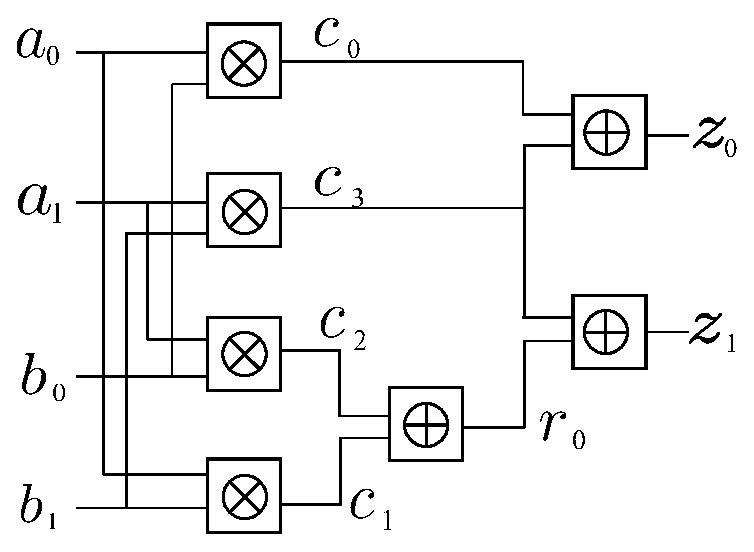
\includegraphics[scale=0.3]{../figures/2bitmultiplier.eps}
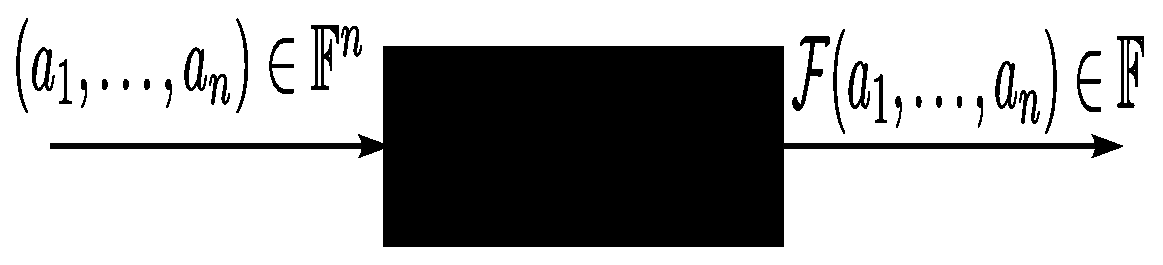
\includegraphics[scale=0.45]{figures/blackbox.eps}
}
\caption{The black-box or the algebraic circuit representation.}
\label{fig:blackbox}
\end{figure}

Let $\Func$ be a multivariate polynomial in $n$ variables $\{x_1, \dots,
x_n\}$, with $t$ non-zero terms ($0 < t < T$), represented with a
black-box $B$. On input $(x_1, \dots, x_n)$,
the black-box evaluates $y_i = \Func(x_1, \dots, x_n)$. Given also a
degree bound $d$ on $\Func$, the goal is to interpolate the polynomial
$\Func$ with a minimum number of {\it probes} to the black-box. The early
work of Zippel \cite{zippel:interpolate} and
Ben-Or/Tiwari \cite{ben-or-tiwari:interpolate} require $O(ndt)$ and
$O(T \log n)$ probes, respectively, to the black-box. These bounds
have since been improved significantly; the recent algorithm of
\cite{monagan:interpolate} interpolates with $O(nt)$ probes.  

Our problem of polynomial abstractions of Galois field circuits 
falls into the category of dense interpolation, as we
require a polynomial that describes the function at each of the $q$
points of the field $\Fq$. Newton's interpolation technique, with the
black-box model, bounds the number of probes by $(d+1)^n$ --- which 
exhibits very high complexity. In the logic synthesis area, the work of
\cite{zilic:interpolate} investigates dense interpolation. Due to this
high-complexity, their approach is feasible only for applications over
small fields, {\it e.g.} computing  Reed-Muller forms for multi-valued
logic over $\F_2$.  

For our problem,
we can also employ the black-box model by replacing the black-box
(algebraic circuit) by the given circuit $C$; then every {\it probe}
of the black-box would correspond to a {\it simulation of the
  circuit}. However, as we desire a polynomial representation of the entire
function over the Galois field, exhaustive simulation would be required, 
which is infeasible.

\section{Concluding Remarks}

For the problem of word-level, canonical, polynomial abstractions
of Galois field arithmetic circuits over $\Fkk$, previous related work 
is either inapplicable or only applicable to circuits no larger than
$32$-bits in size.
Therefore, we propose a {\it symbolic approach} to
polynomial interpolation from a circuit using the Gr\"obner basis
computation. However, the complexity of a \Grobner basis computation is 
prohibitively expensive; thus, we propose further improvements to this 
approach by deriving a smaller subset of computations based on a \Grobner
basis analysis. These improvements allow for abstractions of 
flattened Galois field circuits up to $571$-bits, which is the largest NIST 
standard for ECC, or up to $1024$-bits when a hierarchy is given. 
Furthermore, we propose applications of this 
approach to allow for formal verification of flattened Galois field circuits up to 
$1024$-bits, where current techniques are only applicable for circuits up 
to $163$-bits.

\chapter{Galois Fields Preliminaries and Application in Hardware Design} \label{ch:prelim}
This chapter provides a mathematical background for understanding 
Galois fields and explains how to design Galois field arithmetic circuits.
We first introduce the mathematical concepts of groups, rings, fields, and 
polynomials. 
We then apply these concepts to create Galois field arithmetic functions and 
explain how to map them to a Boolean circuit implementation.
The material is referred from \cite{galois_field:mceliece} \cite{ftheory:2006} \cite{ff:1997} for Galois field concepts and 
\cite{mastro:1989} \cite{PT:1985} \cite{acar:1998} \cite{wu:2002} \cite{Knezevic:2008} for hardware design over Galois fields and previous work
by {\it Lv} \cite{lv:phd}.

%%%%%%%%%%%%%%%%%%%%%%%%%%%%%%%%%%%%%%%%%%%%%%%%%%%%%%%%%%%%%%%%%%%%%%%%%%%%%%%

\section{Rings, Fields and Polynomials}

\begin{Definition}
An {\bf abelian group} is a set $\mathbb{S}$ with a binary operation $'+'$
which satisfies the following properties: 
\begin{itemize}
\item {\it Closure Law:} For every $a, b \in \mathbb{S}, a + b \in \mathbb{S}$  
\item {\it Associative Law:} For every $a, b, c \in \mathbb{S}, (a + b) + c = a + (b + c)$
\item {\it Commutativity:} For every $a, b \in \mathbb{S}, a + b = b + a$. 
\item {\it Additive Identity:} There is an identity element $0 \in \mathbb{S}$
such that for all $a \in \mathbb{S};$ $a + 0 = a$.
\item {\it Additive Inverse:} If $a \in \mathbb{S}$, then there is an
element $a^{-1} \in \mathbb{S}$ such that $ a + a^{-1} = 0$.
\end{itemize}
\end{Definition}

The set of integers $\mathbb{Z}$ forms an abelian group under the addition operation. 

\begin{Definition}
Given a set $\mathbb{R}$ with two binary operations, $'+'$ and $'\cdot'$, 
and element $0 \in \mathbb{R}$, the system $\mathbb{R}$ is called a {\bf commutative ring with unity} if the following properties hold:
\begin{itemize}
\item $\mathbb{R}$ forms an abelian group under the '+' operation with additive identity element $0$.
\item {\it Multiplicative Distributive Law}: For all $a, b, c \in$ $\mathbb{R}$, $a\cdot (b + c) = a\cdot b + a\cdot c$.
\item {\it Multiplicative Associative Law}: For every $a, b, c\in \mathbb{R}$, $a\cdot (b\cdot c) = (a\cdot b)\cdot c$. 
\item {\it Multiplicative Commutative Law}: For every $a,b \in \mathbb{R}$, $a\cdot b = b\cdot a$
\item {\it Identity Element}: There exists an element $1 \in$ $\mathbb{R}$ 
such that for all $a \in \mathbb{R}$, $a\cdot 1 = a =1\cdot a$
\end{itemize}
\end{Definition}

For the purpose of this dissertation, any time we refer to a {\bf ring}, we are 
specifically referring to a {\bf commutative ring with unity}. Two common 
examples of such rings are the set of integers, $\mathbb{Z}$, and the set of 
rational numbers, $\mathbb{Q}$. Note that while both of these examples are
rings with an infinite number of elements, the number of elements in a ring 
can also be finite.

\begin{Definition}
The {\bf modular number system} with base $n$ is a set of positive
integers $Z_n = \{0, 1, \ldots, n-1\}$, with the two operations $+$
and $\cdot$ satisfying the properties below:
\begin{eqnarray}
(a + b)\pmod{ n } &\equiv& ((a ~\pmod {n}) + (b ~\pmod {n})) ~\pmod {n} \nonumber\\
(a\cdot b) ~\pmod {n} &\equiv& ((a ~\pmod {n}) \cdot (b ~\pmod {n})) ~\pmod {n} \label{eq:modmult}\nonumber\\
(-a) ~\pmod {n} &\equiv& (n-a) ~\pmod {n}\nonumber 
\end{eqnarray}
\end{Definition}


\begin{Example}
The set $Z_8 = \{0, 1, \ldots, 7\}$ denotes the modular number system
with base $8$. Examples of some operations performed $\pmod {8}$
are:
\begin{eqnarray} \nonumber
        3 + 6   &~=& 9  ~\pmod{8} ~= 1 \nonumber \\
        3 \cdot 6   &~=& 18 ~\pmod{8} ~= 2 \nonumber \\
        (-3)    &~=& 8-3  ~\pmod{8} ~= 5 \nonumber
\end{eqnarray} \nonumber
\end{Example}

The modular number system $\mathbb{Z}_n = \{0, 1, \ldots, n-1\}$, where $n$ 
is a positive integer, forms a ring.
Since this type of ring contains a finite number of elements $n$,
it is termed a {\it finite integer ring}, where addition and multiplication 
are computed {\it modulo n} $\pmod {n}$. 
In hardware applications, arithmetic over $k$-bit vectors manifests itself 
as algebra over the finite integer ring $\mathbb{Z}_{2^k}$, where the $k$-
bit vector represents integer values from $\{0, ...., 2^k-1\}$.

\begin{Example}
\label{exp:4bitadder}
Consider the following arithmetic circuit:

\begin{figure}[!h]
\centerline{
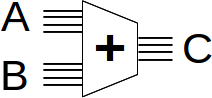
\includegraphics[width=0.3\textwidth]{figures/4bitMultTop}
}
%\caption{Typical hardware design flow.}
%\label{fig:cadflow}
\end{figure}

This circuit takes two 4-bit inputs, $A$ and $B$, and computes a 4-bit sum $C$. 
Since $A$, $B$, and $C$ are all bit-vectors of size $4$, 
the addition computation this circuit performs is modulo $2^4$.
Hence, this circuit exemplifies arithmetic computations over the ring $Z_{2^4}$.

Some examples of possible inputs and outputs of the circuit:
\begin{table}[!h]
	\centering
	\begin{tabular}{|lll|lll|}
	\hline
	\multicolumn{3}{|c|}{Addition over $\mathbb{Z}_{2^4}$} & \multicolumn{3}{c|}{Boolean Circuit Implementation} \\
	\hline
	$5 + 8$ & $~=$ & $13 ~\pmod{16} ~= 13$ & $A=0101$, $B=1000$ & $\rightarrow$ &  $C=1101$ \\
	$10 + 9$ & $~=$ & $ 19 ~\pmod{16} ~= 3$ & $A=1010$, $B=1001$ & $\rightarrow$ &  $C=0011$ \\
	$12 + 4$ & $~=$ & $ 16 ~\pmod{16} ~= 0$ & $A=1100$, $B=0100$ & $\rightarrow$ &  $C=0000$ \\
	\hline
	\end{tabular}
\end{table}
\end{Example}

\begin{Definition}\label{def:poly}
Let $\mathbb{R}$ be a ring. A {\bf polynomial} over $\mathbb{R}$ in the 
indeterminate $x$ is an expression of the form:
\begin{equation} \label{eq:poly1}
a_0 + a_1 x + a_2 x^2 + \cdots + a_k x^k = \sum_{i=0}^{k} a_i x^i, \forall a_i \in \mathbb{R}. 
\end{equation}

\end{Definition}

The constants $a_i$ are the coefficients and $k$ is the degree of the polynomial. 
For example, $8x^3 + 6x + 1$ is a polynomial in $x$ over $\mathbb{Z}$, with
coefficients $8$, $6$, and $1$ and degree $3$. 

\begin{Definition}
The set of all polynomials in the indeterminate
$x$ with coefficients in the ring $\mathbb{R}$ forms a {\bf
ring of polynomials} $\mathbb{R}[x]$. 
Similarly, $\mathbb{R}[x_1,x_{2},\cdots, x_{n}]$ 
represents the ring of multivariate polynomials with coefficients in $\mathbb{R}$.
\end{Definition}

For example, $\mathbb{Z}_{2^4}[x]$ stands for the set of all polynomials in
$x$ with coefficients in $\mathbb{Z}_{2^4}$. $8x^3 + 6x + 1$ is an instance 
of a polynomial contained in $\mathbb{Z}_{2^4}[x]$.

\begin{Definition}
A {\bf field} $\mathbb{F}$ is a commutative ring with unity, where every
non-zero element in $\mathbb{F}$ has a multiplicative inverse; i.e. $\forall
a \in \mathbb{F} - \{0\}$, $\exists \hat{a} \in \mathbb{F}$ such that $ a \cdot
\hat{a} = 1$.
\end{Definition}

A field is defined as a ring with one extra condition: the presence of a 
multiplicative inverse for all non-zero elements.
Therefore, a field must be a ring while a ring is not necessarily a field.
For example, the set $\mathbb{Z}_{2^k} = \{0,1,\cdots, 2^k-1\}$ forms a finite ring.
However, $\mathbb{Z}_{2^k}$ is not a field because not every element in
$\mathbb{Z}_{2^k}$ has a multiplicative inverse. 
In the ring $\mathbb{Z}_{2^3}$, for 
instance, the element $5$ has an inverse ($5\cdot5\pmod{8}=1$) but the element $4$
does not.

The main concept of field theory is {\bf Field Extensions}. The idea behind a
field extension is to take a base field and construct a larger field which 
contains the base field as well as satisfies additional properties. For example,
the set of real numbers $\mathbb{R}$ forms a field; one common extension of 
$\mathbb{R}$ is the set of complex numbers $\mathbb{C}=\mathbb{R}(i)$. Every
element of $\mathbb{C}$ can be represented as $a+b\cdot i$ where $a,b \in \mathbb{R}$,
hence $\mathbb{C}$ is a two-dimensional extension of $\mathbb{R}$.

Like rings, fields can also contain either an infinite or a finite number of 
elements. 
In this dissertation we focus on finite fields, also known as Galois fields, and 
the construction of their field extensions.

%%%%%%%%%%%%%%%%%%%%%%%%%%%%%%%%%%%%%%%%%%%%%%%%%%%%%%%%%%%%%%%%%%%%%%%%%%%%
%%%%%%%%%%%%%%%%%%%%%%%%%%%%%%%%%%%%%%%%%%%%%%%%%%%%%%%%%%%%%%%%%%%%%%%%%%%%
%%%%%%%%%%%%%%%%%%%%%%%%%%%%%%%%%%%%%%%%%%%%%%%%%%%%%%%%%%%%%%%%%%%%%%%%%%%%%
\section{Galois Fields}\label{sec:ff}
Galois fields, also known as finite fields, find widespread applications in 
many areas of electrical engineering and computer science such as error-
correcting codes, elliptic curve cryptography, digital signal processing, 
testing of VLSI circuits, among others.
In this dissertation, we specifically focus on their application to 
Elliptic Curve Cryptography as Galois field arithmetic circuits.
This section describes the relevant Galois field concepts
\cite{galois_field:mceliece} \cite{ftheory:2006} \cite{ff:1997}
and hardware arithmetic designs over such fields \cite{mastro:1989} \cite{PT:1985} 
\cite{acar:1998} \cite{wu:2002} \cite{Knezevic:2008}. 

%%%%%%%%%%%%%%%%%%%%%%%%%%%%%%%%%%%%%%%%%%%%%%%%%%%%%%%%%%%%%%%%%%%%%%%%%%%%

\begin{Definition} 
A {\bf Galois field}, denote $\Fq$, is a field with a finite
number of elements, $q$. The number of elements $q$ of the Galois field is
a power of a prime integer, i.e. $q = p^k$, where $p$ is a prime
integer, and $k \geq 1$. Thus a Galois field can also be denoted as 
$\F_{p^{k}}$.
\end{Definition}

Fields in the form $\F_{p^{k}}$ are called Galois extension fields.
We are specifically interested in extension fields of type 
$\Fkk$, where $k > 1$. These are extensions of the binary
field $\F_2$.
\begin{Example}
Addition and multiplication operations over $\F_2$:
\begin{table}[!h]
	\centering
	\begin{tabular}{m{1cm}|l|ll|m{1cm}}
	\hhline{~---~}
	\multirow{3}{*}{} & $+$ & $0$ & $1$ & \multirow{3}{*}{} \\
	\hhline{~---~}
	& $0$ & $0$ & $1$ & \\
	& $1$ & $1$ & $0$ & \\
	\hhline{~---~}
	\multicolumn{5}{c}{}\\
	\multicolumn{5}{c}{Addition over $\F_2$}\\
	\end{tabular}
	\quad
	\begin{tabular}{m{1cm}|l|ll|m{1cm}}
	\hhline{~---~}
	\multirow{3}{*}{} & $\cdot$ & $0$ & $1$ & \multirow{3}{*}{} \\
	\hhline{~---~}
	& $0$ & $0$ & $0$ & \\
	& $1$ & $0$ & $1$ & \\
	\hhline{~---~}
	\multicolumn{5}{c}{}\\
	\multicolumn{5}{c}{Multiplication over $\F_2$}\\
	\end{tabular}
\end{table}

Notice that addition over $\F_2$ is a Boolean {\sc XOR} operation, 
because it is performed modulo $2$.
Similarly, multiplication over $\F_2$ performs a Boolean {\sc AND} operation.
\end{Example}

Algebraic extensions of the binary field $\F_{2}$  
are generally termed as {\it binary extension fields} $\Fkk$.
Where elements in $\F_2$ can only represent $1$ bit, elements in $\Fkk$ 
represent a $k$-bit vector.
This allows them to be widely used in digital hardware applications.
In order to construct a Galois field of the form $\Fkk$, 
an {\bf irreducible polynomial} is required:
\begin{Definition}
A polynomial $P(x) \in \mathbb{F}_{2}\left[x\right]$ is {\bf irreducible} 
if $P(x)$ is non-constant with degree $k$ and cannot be 
factored into a product of polynomials of lower degree in $\mathbb{F}_2[x]$.
\end{Definition}

Therefore, the polynomial $P(x)$ with degree $k$ is irreducible over 
$\mathbb{F}_{2}$ if and only if it has no roots in $\mathbb{F}_{2}$,
i.e if $\forall a \in \mathbb{F}_{2}$, $P(a)\neq 0$.
For example, $x^2+x+1$ is an irreducible polynomial over $\mathbb{F}_{2}$
because it has no solutions in $\mathbb{F}_{2}$, i.e. $(0)^2+(0)+1=1\neq0$ 
and $(1)^2+(1)+1=1\neq0$ over $\F_2$.
Irreducible polynomials exist for any degree $\geq 2$ in $\mathbb{F}_2[x]$.

Given an irreducible polynomial $P(x)$ of degree $k$ in the polynomial ring 
$\mathbb{F}_2[x]$, we can construct a binary extension field 
$\mathbb{F}_{2^k} \equiv \mathbb{F}_2[x] \pmod{P(x)}$.
Let $\alpha$ be a root of $P(x)$, i.e., $P(\alpha)=0$.
Since $P(x)$ is irreducible over
$\mathbb{F}_2[x]$, $\alpha \notin \mathbb{F}_2$. 
Instead, $\alpha$ is an element in $\mathbb{F}_{2^k}$. 
Any element $A \in \mathbb{F}_{2^k}$ is then represented as: 
\begin{equation}\label{rep:poly}
A= \sum_{i=0}^{k-1} (a_i \cdot \alpha^i) = a_0 + a_1\cdot\alpha + \cdots + a_{k-1}\cdot \alpha^{k-1}\nonumber
\end{equation}
where $a_i \in \mathbb{F}_2$ are the coefficients and $P(\alpha)=0$.

To better understand this field extension, compare its similarities to another
common-place
field extension $\C$, the set of complex numbers. $\C$ is an extension of the field 
of real numbers $\R$ with an additional element $i=\sqrt{-1}$, which is an imaginary
root in $\R$.
Thus $i \notin \R$, rather $i \in \C$.
Every element $A \in \mathbb{C}$ can be represented as:
\begin{equation}\label{rep:polyC}
A=\sum_{j=0}^{1} (a_j \cdot i^j)=a_0+a_1\cdot i
\end{equation}
where $a_j \in \R$ are coefficients. Similarly, $\Fkk$ is an extension of $\F_2$ with 
an additional element $\alpha$, which is the ``imaginary root'' of an irreducible 
polynomial $P$ in $\F_2[x]$.

Every element $A \in \Fkk$ has a degree less than $k$ because 
$A$ is always computed modulo $P(x)$, which has degree $k$. 
Thus, $A\pmod {P(x)}$ can be of degree at most $k-1$ and at least $0$.
For this reason, the field $\mathbb{F}_{2^k}$ can be viewed as a $k$
dimensional vector space over $\mathbb{F}_{2}$. 
The equivalent bit vector representation for element $A$ is:
\begin{equation}
A=(a_{k-1} a_{k-2} \cdots a_{0})
\end{equation}

\begin{Example}
A 4-bit Boolean vector, $(a_{3} a_{2} a_{1} a_{0})$
can be presented over $\F_{2^4}$ as: 
\begin{equation}
a_3 \cdot \alpha^3+a_2 \cdot \alpha^2+a_1 \cdot \alpha+a_0
\end{equation}
For instance, the Boolean vector $1011$ is represented as the element 
$\alpha^3+\alpha+1$.
\end{Example}

\begin{Example}\label{exp:1}
Let us construct $\mathbb{F}_{2^4}$ as $\mathbb{F}_2[x] \pmod{ P(x)}$, where
$P(x)=x^4+x^3+1 \in \mathbb{F}_2[x]$ is an irreducible polynomial of degree $k=4$. 
Let $\alpha$ be the root of $P(x)$, i.e. $P(\alpha)=0$. 

Any element $A \in \mathbb{F}_2[x] \pmod{ x^4 + x^3 + 1}$
has a representation of the type: $A = a_3 x^3 + a_2 x^2 +
a_1 x + a_0$ (degree $< 4$) where the coefficients $a_3, \dots, a_0$ are in $\F_2 =
\{0, 1\}$. Since there are only $16$ such polynomials, we obtain
$16$ elements in the field $\mathbb{F}_{2^4}$. Each element in
$\mathbb{F}_{2^4}$ can then be viewed as a $4$-bit vector over $\mathbb{F}_{2}$. 
Each element also has an exponential $\alpha$
representation. All three representations are shown in Table
\ref{tab:gfelement}.

\begin{table}[h]
\begin{center}
\caption{Bit-vector, Exponential and Polynomial representation of
elements in  $\mathbb{F}_{2^4} = \mathbb{F}_2[x] \pmod{x^4+x^3+1}$}\label{tab:gfelement} 
\begin{tabular}{|c|c|c||c|c|c|} 
\hline
$a_3a_2a_1a_0$ & Exponential & Polynomial     &$a_3a_2a_1a_0$ & Exponential & Polynomial  \\
\hline
$0000$        & $0$         & $0$            & $1000$ & $\alpha^3$ &  $\alpha^3$\\
\hline
$0001$        & $1$         & $1$            & $1001$ & $\alpha^4$ & $\alpha^3 + 1$\\
\hline
$0010$        & $\alpha$    & $\alpha$       & $1010$ & $\alpha^{10}$&$\alpha^3 + \alpha$  \\
\hline
$0011$        & $\alpha^{12}$& $\alpha + 1$   & $1011$ & $\alpha^5$ & $\alpha^3+\alpha+1$\\
\hline
$0100$        & $\alpha^2$  & $\alpha^2$     &  $1100$ & $\alpha^{14}$ & $\alpha^3 + \alpha^2$\\
\hline
$0101$        & $\alpha^9$   &$\alpha^2 + 1$ & $1101$  &$\alpha^{11}$  & $\alpha^3+\alpha^2+1$\\
\hline
$0110$        & $\alpha^{13}$& $\alpha^2 + \alpha$ & $1110$ & $\alpha^8$& $\alpha^3+\alpha^2+\alpha$\\
\hline
$0111$        &$\alpha^7 $ & $\alpha^2+\alpha+1$ & $1111$ &$\alpha^6$ & $\alpha^3+\alpha^2+\alpha+1$\\
\hline
\end{tabular}
\end{center}
\end{table}

We can compute the polynomial representation from the exponential representation.
Since every element is computed $\pmod{P(\alpha)} = \pmod{\alpha^4+\alpha^3+1}$, 
we compute the element $\alpha^{4}$ as 
\begin{equation}
\alpha^{4} \pmod{ \alpha^4+\alpha^3+1} = -\alpha^3 - 1 = \alpha^3+1
\end{equation}
Recall that all coefficients of $\F_{2^4}$ 
are in $\F_{2}$ where $-1 = +1$ modulo 2.
The next element $\alpha^{5}$ can be computed as 
\begin{equation}
\alpha^{5} = \alpha^{4}\cdot \alpha = (\alpha^3+1)\cdot \alpha = \alpha^4+\alpha = \alpha^3+\alpha+1 
\end{equation}
Then $\alpha^6$ can be computed as $\alpha^{5}*\alpha$ and so on.
\end{Example}

An irreducible polynomial can also be a primitive polynomial.

\begin{Definition}
A {\bf primitive polynomial} $P(x)$ is a polynomial with coefficients in $\mathbb{F}_2$ 
which has a root $\alpha$ $\in$ $\mathbb{F}_{2^k}$
such that \{$0$, $1(=\alpha^{{2^k}-1})$, $\alpha$, $\alpha^2$, $\cdots$, $\alpha^{2^k-2}$\} is the set of 
all elements in $\mathbb{F}_{2^k}$, 
where $\alpha$ is a {\bf primitive element} of $\mathbb{F}_{2^k}$. 
\end{Definition}

A primitive polynomial is guaranteed to generate all distinct elements 
of a finite field $\mathbb{F}_{2^k}$ while an irreducible polynomial
has no such guarantee.
Often, there exists more than one irreducible polynomial of degree $k$.
In such cases, any degree $k$ irreducible polynomial can be 
used for field construction. For example, both $x^3+x+1$ and $x^3+x^2+1$ 
are irreducible in $\mathbb{F}_2$ and either one can be used
to construct $\mathbb{F}_{2^3}$. This is due to the following:

\begin{Theorem}\label{the:unique}
There exist a {\bf unique} field $\mathbb{F}_{p^k}$, for any prime $p$ and any positive integer $k$.
\end{Theorem}

Theorem \ref{the:unique} implies that Galois fields with the same number of elements are 
{\bf isomorphic} to each other up to the labeling of the elements. 

Theorem \ref{the:fer} provides an important property for investigating solutions to
polynomial equations in $\Fq$.

\begin{Theorem}\label{the:fer}
 $\left[Generalized\  Fermat's\  Little\  Theorem \right]$ Given a
 Galois field $\mathbb{F}_{q}$, each element $A \in \mathbb{F}_{q}$ satisfies: 
\begin{eqnarray}\label{fe}
 A^{q} & \equiv & A  \nonumber \\
 A^{q} - A & \equiv& 0  
\end{eqnarray}
\end{Theorem} 

We can extend Theorem \ref{the:fer} to polynomials in $\mathbb{F}_{q}[x]$ as 
follows: 
\begin{Definition}
Let $x^q-x$ be a polynomial in $\mathbb{F}_{q}[x]$.
Every element $A \in \mathbb{F}_{q}$ is a solution to  $x^q-x=0$. 
Therefore, $x^{q} - x$ always {\it vanishes} in $\mathbb{F}_{q}$. Such 
polynomials are called {\bf vanishing polynomials} of the field $\mathbb{F}_{q}$.
\end{Definition}

\begin{Example}
Given $\mathbb{F}_{2^2} =\{0,1,\alpha,\alpha+1\}$ with $P(x)=x^2+x+1$, where $P(\alpha)=0$. 
 \begin{eqnarray}
 0^{2^2}&=&0 \nonumber \\
 1^{2^2}&=&1 \nonumber \\
 \alpha^{2^2}&=&\alpha \pmod {\alpha^2+\alpha+1}\nonumber \\
 (\alpha+1)^{2^2}&=&\alpha+1 \pmod {\alpha^2+\alpha+1} \nonumber 
 \end{eqnarray}
\end{Example}

%%%%%%%%%%%%%%%%%%%%%%%%%%%%%%%%%%%%%%%%%%%%%%%%%%%%%
\subsection{Containment of Galois Fields}
A Galois field $\F_q$ can be fully contained within a larger field $\F_{q^k}$.
That is, $\F_q \subset \F_{q^k}$.
For example, Fig \ref{fig:contain2_4_16} shows the containment of the fields 
$\F_2 \subset \F_4 \subset \F_{16}$. It's easy to see that since $\F_4=\F_{2^2}$, it
contains $\F_2$. Likewise $\F_{16}=\F_{4^2}=\F_{2^4}$ contains $\F_4$ and $\F_2$.
The elements $\{0,1,\alpha,\dots,\alpha^{14}\}$
designate $\F_{16}$. Of these, $\{0,1,\alpha^5,\alpha^{10}\}$ create $\F_4$.
From these, only $\{0,1\}$ exist in $\F_2$.

\begin{figure}[H]
\begin{center}
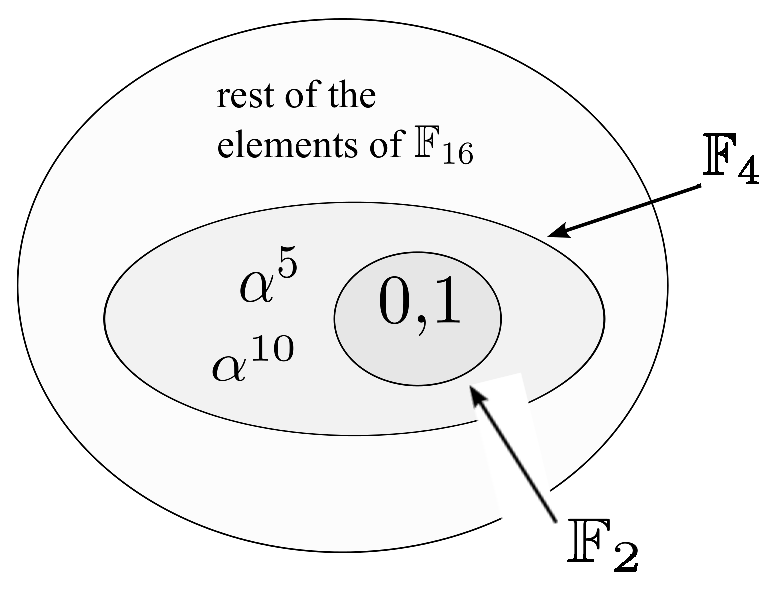
\includegraphics[scale=0.7]{./figures/field-cont}
\end{center}
\caption{Containment of Fields: $\F_2 \subset \F_4 \subset \F_{16}$}
\label{fig:contain2_4_16}
\end{figure}

Consider the element $\alpha^5$ of $\F_{16}$. 
Deriving all $(\alpha^5)^i$ for $i \geq 0$ 
over $\F_{16}$ gives the following recurrence:
\begin{eqnarray}
(\alpha^5)^0&=&1\nonumber \\
(\alpha^5)^1 &=& \alpha^5\nonumber \\
(\alpha^5)^2 &=& \alpha^{10}\nonumber \\
(\alpha^5)^3 &=& \alpha^{15} = 1
\end{eqnarray}
The only elements that are generated in this recurrence are $\{1,\alpha^5,\alpha^{10}\}$.
Every field contains $\{0,1\}$, so the elements $\{0,1,\alpha^5,\alpha^{10}\}$ form $\F_4$.
Let $P(x)=x^4+x^3+1$ be the primitive polynomial used to generate
$\F_{2^4}=\F_{16}$. A primitive polynomial of degree $2$ used to generate $\F_{2^2}=\F_4$
can be found as follows:
\begin{eqnarray}
& &(x+\alpha^5)\cdot(x+\alpha^{10}) \mod P(x) \nonumber \\
&=& x^2+(\alpha^{10}+\alpha^5)x+\alpha^{15} \mod P(x) \nonumber \\
&=& x^2+x+1
\end{eqnarray}

\begin{Theorem}
$\F_{2^n}\subset\F_{2^m}$ iff $n \mid m$, i.e. if $n$ divides $m$.
\end{Theorem}

Therefore:
\begin{itemize}
\item $\F_2 \subset \F_{2^2} \subset \F_{2^4} \subset \F_{2^8} \subset \dots$
\item $\F_2 \subset \F_{2^3} \subset \F_{2^9} \subset \F_{2^{27}} \subset \dots$
\item $\F_2 \subset \F_{2^5} \subset \F_{2^{25}} \subset \F_{2^{125}} \subset \dots,$ and so on
\end{itemize}

\begin{Definition}
The {\bf algebraic closure} of the Galois field $\F_{2^k}$, denoted $\overline{\Fkk}$, is the 
union of all fields $\F_{2^n}$ such that $k \mid n$.
\end{Definition}


%%%%%%%%%%%%%%%%%%%%%%%%%%%%%%%%%%%%%%%%%%%%%%%%%%%%%%
\subsection{Polynomial Interpolation over Galois Fields}

In the construction of digital circuits, arbitrary mappings between 
two bit-vectors of size $k$ can be constructed. Each such
mapping generates a function $f: \B^k \rightarrow \B^k$.
As every $k$-bit vector can be construed as an element in $\Fkk$ 
(as shown in the previous section), 
every such function also corresponds to a function over a 
Galois field: $f: \Fkk \rightarrow \Fkk$. 

\begin{Definition}
A function $f: \mathbb{R} \rightarrow \mathbb{R}$ over a ring $R$ is 
considered a {\bf polynomial function} if there exists a polynomial
$\Func \in \mathbb{R}[x_1,\dots,x_d]$ such that 
$\Func(x_1,\dots,x_d) = f(x_1,\dots,x_d)$.
\end{Definition}

\begin{Theorem}
From \cite{ff:1997}: 
Let $\Fq$ be a Galois field of $q$ elements where $q$ is a power of a
prime integer. Given any function $f: \Fq \to \Fq$, there exists a 
polynomial 
$\Func \in \Fq [x]$ such that $f(a) = \Func(a)$, for all $a \in \Fq$.
Thus, every function $f: \Fq \to \Fq$ is a polynomial function.
\end{Theorem}

Thus, since every function over a Galois field, $f: \Fkk \rightarrow \Fkk$, 
is a polynomial function, 
every mapping between two bit-vectors of size $k$ 
is a polynomial function over $\Fkk$.
Furthermore, every polynomial can be derived using Lagrange interpolation.

\begin{Theorem} ({\bf Lagrange Interpolation}): \\
Given a set of $k$ data points over a function $f$,
\begin{equation}
(x_0,f(x_0)),\dots,(x_{k-1},f(x_{k-1})) \nonumber
\end{equation}
where no two $x_i \in \{x_0,\dots,x_{k-1}\}$ are the same elements,
the polynomial representation of $f$, $\Func(x)$, can be interpolated as 
follows:  
\begin{eqnarray}
\Func(x) = \sum_{i=0}^{k-1} f(x_i)\cdot L_i(x) \nonumber \\
L_i(x) =  \prod_{(0\leq j \leq k-1),(j\neq i)}\frac{x-x_j}{x_i-x_j} \nonumber  
\end{eqnarray}
\end{Theorem}

By applying Lagrange interpolation over every element in the Galois
field $\Fkk$, 
we can derive the polynomial representation $\Func$ of any function 
$f:\Fkk \rightarrow \Fkk$. Furthermore, $\Func$ is a polynomial of degree 
at most $2^k-1$ in $x$ and $\Func(a)=f(a)$ for all $a \in \Fkk$.

While every function over a Galois field is a polynomial function,
not every function over the integer ring $\mathbb{Z}$ is a polynomial 
function.


%\begin{equation}
%\Func(x) = \sum_{k=1} ^q  \frac{ \prod_{i \neq k}  (x -x_i)}{\prod_{i \neq k}(x_k -x_i)} \cdot \f(x_k)
%\label{eqn:lagrange}
%\end{equation}

%As every function over a Galois field is also a polynomial 
%function, any mapping between two $k$-bit vectors is also a 
%polynomial function when analyzed over $\Fkk$.

%By analyzing $\Func$ over each point in $\Fq$ and applying 
%{\bf Lagrange's interpolation formula}, shown in 
%Equation \ref{eqn:lagrange}, one can interpolate the 
%polynomial representation, $f_p$, of the function $\Func$.

%Then, $f_p$ is a polynomial of degree at most $q-1$ in $x$ and
%$f_p = \F(a)$ for all $a \in \Fq$, and $\F(x)$.
%Thus, $f_p$ is a polynomial function representation of $\Func$. 


\begin{Example} {\it
Let $A = \{a_2, a_1, a_0\}$ and $Z = \{z_2,z_1,z_0\}$ be 3-bit vectors.
Thus, $A$ and $Z \in \mathbb{B}^3$. 
Consider the following function:
\begin{equation}
f:Z[2:0] = A[2:0]>>1 \nonumber
\end{equation}
$f$ is a {\bf bit-vector right shift} operation on $A$. 
This function can be analyzed as a mapping over different forms: 
$\mathbb{B}^3 \rightarrow \mathbb{B}^3$,
$\mathbb{Z}_8 \rightarrow \mathbb{Z}_8$, and
$\F_{2^3} \rightarrow \F_{2^3}$. These mappings from $A$ to $Z$ 
are:

\begin{center}
{\small
\begin{tabular}{c|c|ccc|c|c|} 
$\{a_2a_1a_0\}\in\mathbb{B}^3$  & $A\in \mathbb{Z}_8$ & $A\in \F_{2^3}$ &$\rightarrow$& $\{z_2z_1z_0\}\in\mathbb{B}^3$ &$Z\in \mathbb{Z}_8$ & $Z\in \F_{2^3}$ \\
\hline
000  &0&0 &$\rightarrow$&000 &0& 0 \\
001  &1&1 &$\rightarrow$&000 &0& 0 \\
010  &2&$\alpha$ & $\rightarrow$ & 001&1& 1 \\
011  &3&$\alpha + 1$ &$\rightarrow$& 001&1 &1 \\
100  &4&$\alpha^2$ &$\rightarrow$& 010 &2&  $\alpha$ \\
101  &5&$\alpha^2 + 1$ &$\rightarrow$&010 &2& $\alpha$ \\
110  &6&$\alpha^2 + \alpha$&$\rightarrow$& 011 &3&$\alpha + 1$ \\
111  &7&$\alpha^2 + \alpha + 1$ &$\rightarrow$& 011 &3&$\alpha + 1$\\
\hline
\end {tabular}
}
\end{center}

$f: \mathbb{Z}_8 \rightarrow \mathbb{Z}_8$ is not a polynomial function 
(this can be verified using the results of \cite{singmaster}
\cite{chen_95} \cite{chen_96}). However, $f: \F_{2^3} \rightarrow \F_{2^3}$
is a polynomial function.
By applying Lagrange's interpolation formula to $f$ over $\F_{2^3}$ for 
every element in $\F_{2^3}$, 
we obtain the following polynomial function: $Z =
(\alpha^2+1)A^4+(\alpha^2+1)A^2$, where $P(\alpha) = \alpha^3 +
\alpha + 1 = 0$. 
}
\end{Example}

Since every function over $\Fkk$ is a polynomial function, the 
functional mapping of a Galois field arithmetic circuit over
$\Fkk$ must exist in polynomial form. 
Construction of these arithmetic circuits is described next.


%%%%%%%%%%%%%%%%%%%%%%%%%%%%%%%%%%%%%%%%%%%%%%%%
%%%%%%%%%%%%%%%%%%%%%%%%%%%%%%%%%%%%%%%%%%%%%%%%
%%%%%%%%%%%%%%%%%%%%%%%%%%%%%%%%%%%%%%%%%%%%%%%%
\section{Hardware Implementations of Arithmetic Operations Over Galois Fields}

There are two main applications of hardware implementations of Galois field 
arithmetic.
In the first case, Galois field arithmetic computations, such as {\sc add or mul},  
are implemented in hardware, and  
algorithms are then implemented in software 
(e.g. cryptoprocessors \cite{ST23} \cite{kobayashi}). 
In other cases, the entire design can be implemented in hardware, such as a one-shot 
Reed-Solomon encoder-decoder chip \cite{reed-solo-chip} \cite{ecc163}, or point 
multiplication circuitry \cite{ecc:software} used in elliptic curve cryptosystems. 
Therefore, there has been extensive research in efficient hardware design of 
primitive arithmetic computations over Galois fields.
In this section, we describe the design principles of such circuits with focus 
on their architecture and verification complexity.

{\bf Addition} in $\Fkk$ is performed by correspondingly adding the
polynomials together and reducing the coefficients of the result modulo $2$.
\begin{Example}
Given $A=\alpha^3+\alpha^2+1=(1101) $ and $B=\alpha^2+1=(0101)$ in $\mathbb{F}_{2^4}$, 
\begin{equation}
A+B=(\alpha^3+\alpha^2+1)+(\alpha^2+1)=(\alpha^3) + (\alpha^2+\alpha^2) +(1+1)=\alpha^3=(1000). \nonumber
 \end{equation}
\end{Example}

Effectively, the addition operation is only performed on the coefficients, 
which are in $\F_2$. 
As addition over $\F_2$ performs an {\it XOR} operation,
constructing an addition circuit over $\Fkk$ is trivial as it
only consists of $k$ number of {\it XOR} gates. 
A $4$-bit adder over $\F_{2^4}$ is shown in
Fig. \ref{fig:adder4}.
\begin{figure}[H]
\begin{center}
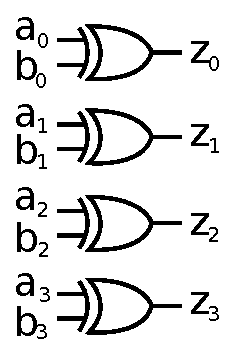
\includegraphics[scale=0.6]{figures/adder4bit}
\end{center}
\caption{$4$-bit adder over $\mathbb{F}_{2^4}$.}
\label{fig:adder4}
\end{figure}

{\bf Multiplication} $Z =A\times B \pmod{ P(x) }$ in $\Fkk$ conceptually consists of 
two steps.
In the first step, the multiplication $A\times B$ is performed. In the second 
step, the result is reduced
modulo the irreducible polynomial $P(x)$.
This multiplication procedure is shown in Example \ref{exp:mul}.

%\ref{exp1}, 
\begin{Example}
\label{exp:mul}
Consider the field $\mathbb{F}_{2^4}$ with the irreducible polynomial 
$P(x)=x^4+x^3+1$ and $P(\alpha)=0$. We take as inputs:
$A=a_0+a_1\cdot \alpha+a_2\cdot \alpha^2+a_3\cdot \alpha^3$ and
$B=b_0+b_1\cdot \alpha+b_2\cdot \alpha^2+b_3\cdot \alpha^3$. 
We have to perform the multiplication $Z =A\times B \pmod{ P(x) }$. The coefficients
of $A = \{a_0, \dots, a_3\}, B = \{b_0, \dots, b_3\}$ are in
$\mathbb{F}_2 = \{0, 1\}$. This multiplication can be performed as
shown:

{\begin{tabular}{c c c c c c c c}
  &   &   & $a_3$ & $a_2$ & $a_1$ & $a_0$  \\ 
 $\times$&   &   & $b_3$ & $b_2$ & $b_1$ & $b_0$  \\ 
 \hline
 &   &   & $a_3\cdot b_0$ & $a_2 \cdot b_0$ & $a_1\cdot b_0$ & $a_0\cdot b_0$ \\
 &  & $a_3\cdot b_1$ & $a_2\cdot b_1$ & $a_1 \cdot b_1$ & $a_0\cdot b_1$ &   \\
 & $a_3\cdot b_2$ & $a_2\cdot b_2$ & $a_1\cdot b_2$ & $a_0\cdot b_2$ &  &   \\
 $a_3\cdot b_3$ & $a_2\cdot b_3$ & $a_1\cdot b_3$ & $a_0\cdot b_3$ &  &  &   \\
 \hline
 $s_6$& $s_5$  & $s_4$  & $s_3$ & $s_2$  & $s_1$   & $s_0$ 
\end{tabular}}

The result $Sum = s_0+s_1\cdot \alpha + s_2\cdot \alpha^2 + s_3\cdot
\alpha^3 + s_4\cdot \alpha^4 + s_5\cdot \alpha^5 + s_6\cdot \alpha^6$,
where
\begin{eqnarray}
	s_0  &=&  a_0\cdot b_0 \nonumber \\ 
	s_1  &=&  a_0\cdot b_1 + a_1\cdot b_0 \nonumber \\
	s_2  &=&  a_0\cdot b_2 + a_1\cdot b_1 + a_2\cdot b_0 \nonumber \\
	s_3  &=&  a_0\cdot b_3 + a_1\cdot b_2 + a_2\cdot b_2 +  a_3\cdot b_1\nonumber \\
	s_4  &=&  a_1\cdot  b_3 + a_2\cdot b_1 + a_3\cdot b_1 \nonumber \\
	s_5  &=&  a_2\cdot b_3 + a_3\cdot b_2  \nonumber \\
	s_6  &=&  a_3\cdot b_3   \nonumber
\end{eqnarray}
 Here the multiply ``$\cdot$'' and add ``$+$'' operations are performed
modulo 2, so they can be implemented in a circuit using AND and XOR
gates respectively. Note that unlike integer multipliers, there are no carry-chains
in the design, as the coefficients are always reduced modulo $2$. 
However, the result is yet to be reduced modulo the primitive
polynomial $P(x) = x^4 + x^3 + 1$. This transforms every exponent representation, 
$\alpha^d$, to a polynomial representation where $d\geq k=4$.

{\begin{tabular}{|c c c c | l }
 \multicolumn{5}{c}{} \\
 \multicolumn{1}{c}{$\alpha^3$} & $\alpha^2$ & $\alpha$ & \multicolumn{1}{c}{$1$} &  \\
\hhline{----~}
  $s_3$ 	&$s_2$  	&$s_1$   &$s_0$ 	&   \\
 \hline
 $s_4$ 		&$0$		&$0$ 	 &$s_4$  	&$s_4\cdot \alpha^4 \pmod{P(\alpha)} = s_4 \cdot (\alpha^3 + 1)$\\
 $s_5$ 		&$0$		&$s_5$   &$s_5$     &$s_5\cdot \alpha^5 \pmod{P(\alpha)} = s_5\cdot (\alpha^3+ \alpha + 1)$\\
 $s_6$ 		&$s_6$		&$s_6$   &$s_6$     &$s_6\cdot \alpha^6 \pmod{ P(\alpha)} = s_6\cdot( \alpha^3 + \alpha^2 + \alpha + 1)$\\
 \hline
 $z_3$ 		&$z_2$ 		&$z_1$   &$z_0$ 	&\\
 \multicolumn{5}{c}{} \\
 \end{tabular}\par}

The final result (output) of the circuit is: $Z = z_0 + z_1 \alpha + z_2
\alpha^2 + z_3 \alpha^3$; where  $z_0=s_0+s_4+s_5+s_6; ~~z_1=s_1+s_5+s_6;
~~z_2=s_2+s_6; ~~z_3=s_3+s_4+s_5+s_6$. 
\end{Example}

%%%%%%%%%%%%%%%%%%%%%%%%%%%%%%%%%%%%%%%%%%%%%%%%%%%%%%%%%%%

The above multiplier design is called the {\it Mastrovito multiplier} \cite{mastro:1989} 
which is the most straightforward way to design a multiplier over $\mathbb{F}_{2^k}$. 
A logic circuit for a $4$-bit {\it Mastrovito} multiplier over {\it Galois field} $\mathbb{F}_{2^4}$ is illustrated in Fig. \ref{fig:mas4}.

\begin{figure}[H]
	\begin{center}
	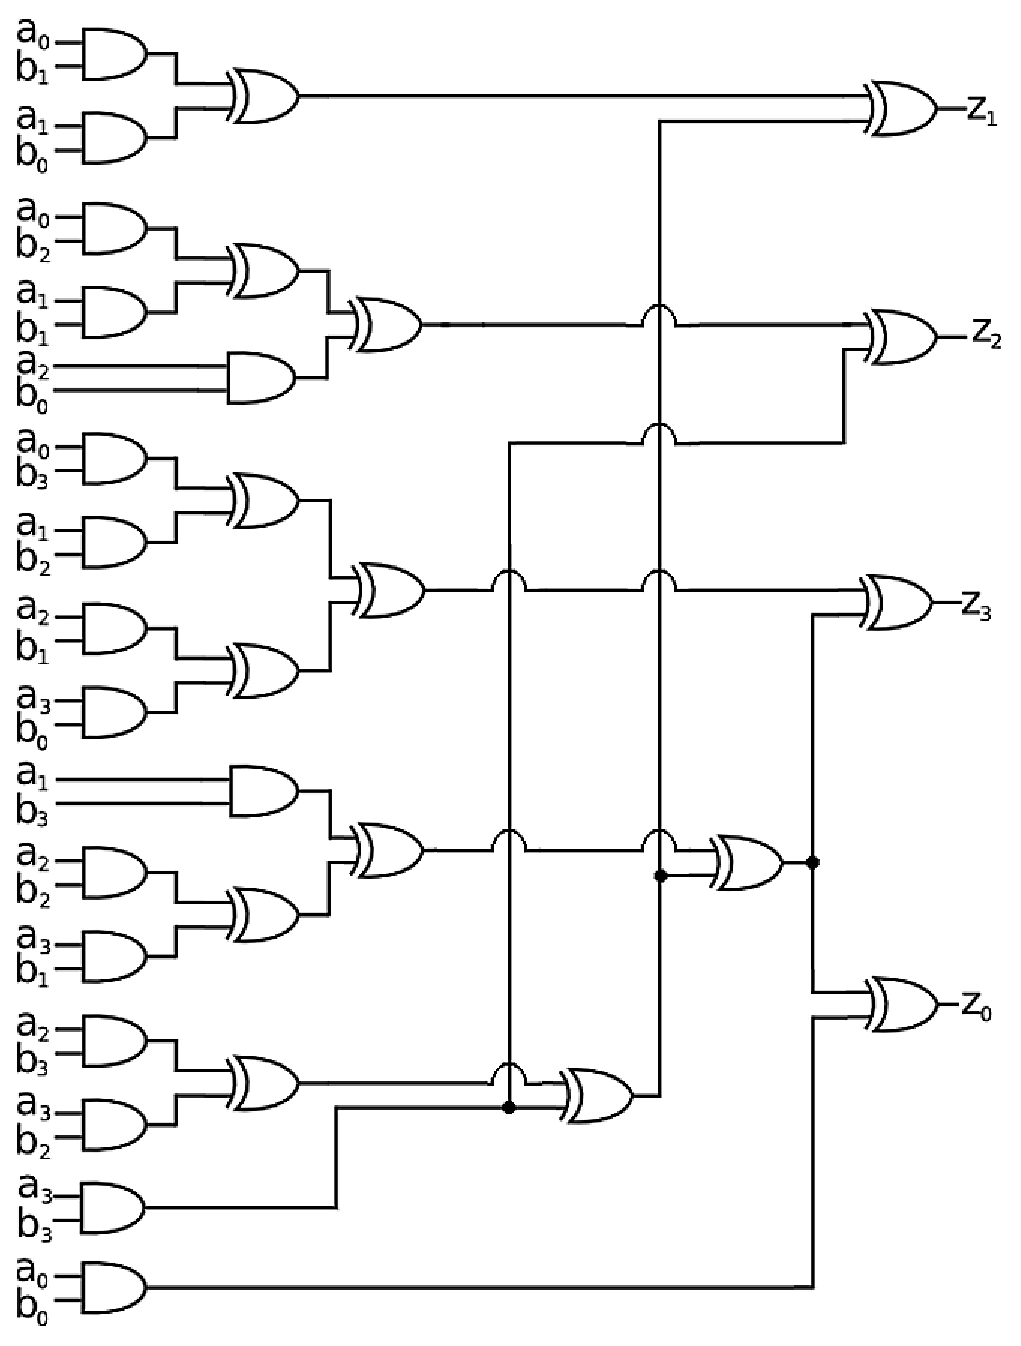
\includegraphics[scale=0.60]{figures/mul4bit.eps}
	\end{center}
	\caption{Mastrovito multiplier over $\mathbb{F}_{2^4}$.}
	\label{fig:mas4}
\end{figure}

Modular multiplication is at the heart of many public-key cryptosystems, 
such as Elliptic Curve Cryptography (ECC) \cite{ecc:1986}. 
Due to the very large field size (and hence the data-path width) used in these cryptosystems, 
the above {\it Mastrovito} multiplier architecture is inefficient, especially when 
exponentiation and repeat multiplications are performed.
Therefore, efficient hardware and software implementations of modular multiplication 
algorithms are used to overcome the complexity of such operations. 
One such algorithm which we will focus on is the Montgomery reduction \cite{PT:1985} \cite{acar:1998}.

\subsection{Montgomery Multipliers}
Montgomery Reduction (MR) computes: 

\begin{equation}
G=MR(A,B)=A\cdot B \cdot R^{-1} \pmod {P(x)}
\end{equation}
where $A,B$ are $k$-bit inputs, $R={\alpha}^k$, $R^{-1}$ is multiplicative
inverse of $R$ in $\mathbb{F}_{2^k}$, and $P(x)$ is the irreducible polynomial for
$\mathbb{F}_{2^k}$. Since Montgomery reduction cannot directly compute $A\cdot B$, 
we need to pre-compute $A\cdot R$ and $B\cdot R$,
as shown in Fig. \ref{fig:mm4}.  

\begin{figure}[h]
	\begin{center}
	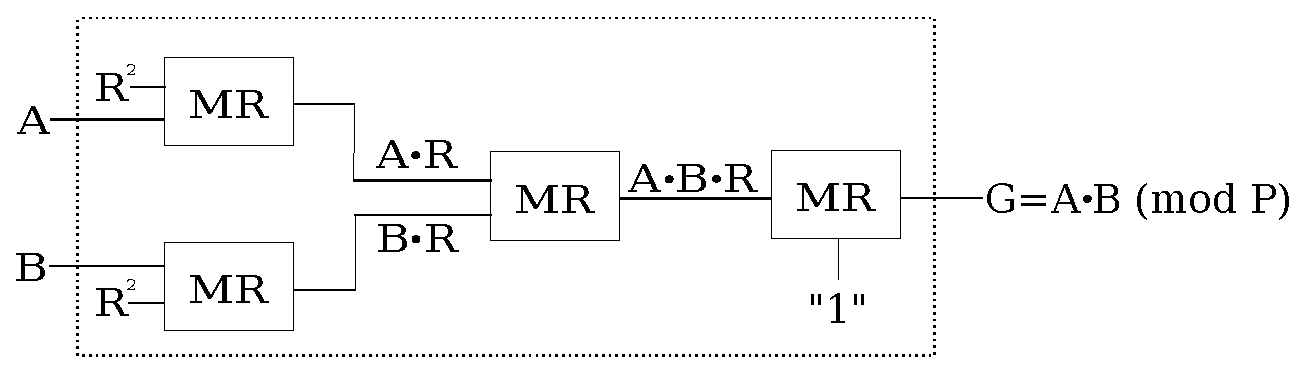
\includegraphics[scale=0.50]{figures/mmcircuit}
	\end{center}
	\caption{Montgomery multiplier over $\mathbb{F}_{2^k}$}
	\label{fig:mm4}
\end{figure}

Each $\it MR$ block in Fig. \ref{fig:mm4} represents a Montgomery reduction step 
which is a hardware implementation of the algorithm shown in 
Algorithm \ref{alg:mont}. 

\begin{algorithm}
\SetAlgoNoLine

 \KwIn{$A(x), B(x)\in \mathbb{F}_{2^k}$; irreducible polynomial $P(x)$.}
 \KwOut{$G(x)=A(x)\cdot B(x)\cdot x^{-k} \pmod {P(x)}$.}
%%%%%%%%%%%%%%%%%%%%
  $G(x):=$0 \\
  \For { ($i=0$;   $i \le k-1$; ++i ) }
  {
	$G(x):=G(x)+A_i\cdot B(x)$ \CommentSty{/*$A_{i}$ is the $i^{th}$ bit of $A$*/\;}
	$G(x):=G(x)+G_0\cdot P(x)$ \CommentSty{/*$G_{0}$ is the lowest bit of $G$*/\;}
	$G(x):=G(x) / x$ \CommentSty{/*Right shift $1$ bit*/\;}
  }
\caption{Montgomery Reduction Algorithm \cite{acar:1998}}\label{alg:mont}
\end{algorithm}

The design of Fig. \ref{fig:mm4} is not efficient to computing
$A\cdot B \pmod{ P(x)}$ when compared to the Mastrovito implementation.
However, when these multiplications are
performed repeatedly, such as in iterative squaring, then the
Montgomery approach speeds-up the computation. 
As shown in \cite{wu:2002}, the critical path delay and gate counts of a squarer 
designed using the Montgomery approach are much smaller than the traditional 
approaches.

\subsection{Circuit Designs over Composite Fields}
The Galois field $\mathbb{F}_{2^k}$ is a $k$-dimensional vector space over the
sub-field $\mathbb{F}_2$. If $k = m\cdot n$, the field $\mathbb{F}_{2^k}$
can be decomposed as $\mathbb{F}_{(2^m)^n}$. Such a field representation is
called a {\bf composite field}, and it is constructed as a $n$-dimensional 
extension of the sub-field $\mathbb{F}_{2^m}$. The sub-field $\mathbb{F}_{2^m}$ is
called the ground field. Note that we have $\mathbb{F}_2 \subset \mathbb{F}_{2^m}
\subset \mathbb{F}_{(2^m)^n}$.

A Galois field arithmetic circuit over $\Fkk$ can thus be composed
as circuit over $\F_{(2^m)^n}$ if $k=m\cdot n$.
Since the base field is $\F_{2^m}$, this composite field circuit is
composed of blocks of $m$-bit multipliers and adders, along with 
$m$-bit buses that act as the inputs and outputs of these blocks.
A $\F_{2^4}$ Galois field multiplier designed over the composite field $\F_{(2^2)^2}$ is shown in 
Fig. \ref{fig:comp4exPrelim}.
Design methodologies of these circuits are examined more closely in Chapter \ref{ch:generalize}.

\begin{figure}[t]
        \centering
        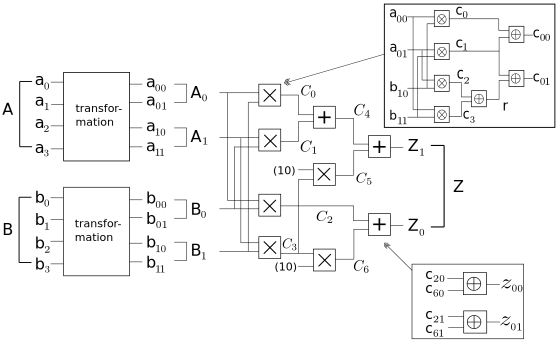
\includegraphics[width=.9\linewidth]{./figures/compMineSmall}
        \caption{$4$-bit composite multiplier designed over $\F_{(2^2)^2}$}\label{fig:comp4exPrelim}
\end{figure}

%% According to Theorem \ref{the:unique}, there exists an unique field of size $p^{k}$. 
%% This implies that $\mathbb{F}_{2^k}$ is isomorphic to
%% $\mathbb{F}_{(2^m)^n}$ when $k = m\cdot n$, and due to this isomorphism,
%% it is possible to derive one field representation from the other. 
%% The principle of constructing a composite field is described in \cite{phdpaar:1994}. 
%% We derive concrete steps for constructing circuits over composite fields.

%% To construct $\mathbb{F}_{(2^m)^n}$, we require a primitive polynomial of 
%% degree $n$, with coefficients from the ground field $\mathbb{F}_{2^m}$. 
%% Let $k=m\cdot n$. Given $\mathbb{F}_{2^k}$ and its primitive polynomial $P(x)$
%% of degree k, 
%% the primitive polynomial of the composite field can be easily
%% derived. We use the following notation:

%% \begin{itemize}
%% \item Let $P(x)$ denote the given primitive polynomial of general
%%   field $\mathbb{F}_{2^k}$. Let $\alpha$ be a root of the 
%%   this polynomial, i.e. $P(\alpha)=0$.  
%% \item Let $Q(x)$ denote the primitive polynomial of ground field
%%   $\mathbb{F}_{2^m}$. Let $\beta$ be a root of $\mathbb{F}_{2^m}$,
%%   i.e. $Q(\beta)=0$. Note that $Q(x)$ is a degree $m$ primitive
%%   polynomial over $\mathbb{F}_{2}$ so it is also known. 
%% \item Let $R(x)$ denote the primitive polynomial of composite field
%%   $\mathbb{F}_{(2^m)^n}$. Let $\gamma$ be a root,
%%   i.e. $R(\gamma)=0$. This polynomial $R(x)$ has to be derived. 
%% \end{itemize}

%% %To construct $R(x)$, we hae the following result 
%% \begin{Lemma}
%% From \cite{cf:2003}: Let $\mathbb{F}_{2^k}$ be decomposed as $\mathbb{F}_{(2^m)^n}$
%% where $k = m\cdot n$. Let $\gamma$ be the primitive root of the field $\mathbb{F}_{(2^m)^n}$. 
%% Then 
%% \begin{equation}
%% R(x)=\prod_{i=0}^{i=n-1}(x_i+\gamma^{2^{m \cdot i}})
%% \end{equation}
%% \end{Lemma}

%% Since $\mathbb{F}_{2^k}$ is isomorphic to $\mathbb{F}_{(2^m)^n}$, $\alpha$ and
%% $\gamma$ are the same elements ($\alpha=\gamma$).
%% Consider the representation of an element $A$ in $\mathbb{F}_{2^k}$ and its corresponding
%% representation in the composite field.

%% \begin{itemize}
%% \item Any element $A \in \mathbb{F}_{2^k}$ is represented as:
%% \begin{equation}
%% A=\sum_{i=0}^{i=k-1}a_i \cdot \alpha^i, a_i \in \mathbb{F}_{2}, \text{and}\	 P(\alpha) = 0
%% \end{equation}
%% \item The same element $A \in \mathbb{F}_{(2^m)^n}$ is represented as:
%% \begin{equation}
%% A=\sum_{i=0}^{i=n-1}A_i \cdot \gamma^i, A_i \in \mathbb{F}_{2^m}, \text{and} \	 R(\gamma) = 0
%% \end{equation}
%% \item The element $A_i$ needs to be represented in the ground field $\mathbb{F}_{2^m}$:
%% \begin{equation}
%% A_i=\sum_{j=0}^{j=m-1}a_{ij} \cdot \beta^j, a_{ij} \in \mathbb{F}_{2}, \text{and} \	 Q(\beta) = 0
%% \end{equation}
%% \end{itemize}

%% Thus, we need to find the relationship between the primitive roots
%% $\alpha$ and $\beta$ (or between $\gamma$ and $\beta$, since $\alpha =\gamma$), 
%% so as to be able to map the elements from $\mathbb{F}_{2^k}$ to $\mathbb{F}_{(2^m)^n}$. 
%% We use the following result \cite{cf:2003}:

%% \begin{Theorem}\label{thm:gamma}
%% For $\gamma \in \mathbb{F}_{(2^m)^n}$, and $\beta=\gamma^{\omega}$, where $\omega=(2
%% ^{m \cdot n}-1)/(2^m-1)$, then we have $\beta \in \mathbb{F}_{2^m}$. In other
%% words: 
%% \begin{equation}
%% \beta=\alpha^{(2^{m \cdot n}-1)/(2^m-1)}=\gamma^{(2^{m \cdot n}-1)/(2^m-1)} \label{eqn:relation}
%% \end{equation}

%% \end{Theorem}

%% The above result states the following: Since $\gamma$ is a primitive
%% root, it can be used to generate all the non-zero elements of $\mathbb{F}_{(2^m)^n}$. 
%% Moreover, $\beta$ is a primitive root of the ground field $\mathbb{F}_{2^m}$, 
%% which is a sub-field of $\mathbb{F}_{(2^m)^n}$ ( i.e. $\mathbb{F}_{2^m}
%% \subset \mathbb{F}_{(2^m)^n}$); so $\beta \in \mathbb{F}_{(2^m)^n}$. Therefore
%% an exponent of $\gamma$ can be used to generate $\beta$ as
%% $\beta=\gamma^{\omega}$, where $\omega$ is given in Theorem
%% \ref{thm:gamma}. Now that we have all the relationships between $\alpha,
%% \beta, \gamma$, it is possible to perform the decomposition. 

%% \begin{Example}
%% Consider the field $\mathbb{F}_{2^4}$ 
%% with $P(x) = x^4 + x^3 + 1$ and $P(\alpha)=0$.
%% In order to decompose it as $\mathbb{F}_{(2^2)^2}$,
%% perform the following steps:

%% \begin{enumerate}
%% \item 
%% Derivation of $R(x)$:
%% \begin{eqnarray}
%% R(x)&=&\prod_{i=0}^{i=1}(x+\gamma^{2^{2 \cdot i}}) \nonumber \\
%% &=&(x+\gamma)\cdot (x+\gamma^{2^2})               \nonumber \\
%% &=&x^2+(\gamma^4+\gamma) \cdot x+\gamma^5          
%% \end{eqnarray}
%% Notice that $R(\gamma) = \gamma^2 + (\gamma^4+\gamma) \cdot \gamma+\gamma^5 =0$.
%% \item 
%% Representation of element $A \in \mathbb{F}_{(2^2)^2}$:
%% \begin{eqnarray}
%% A& = & \sum_{i=0}^{i=1}A_i \cdot \gamma^i, A_i \in \mathbb{F}_{2^2}\nonumber \\
%%  & = & A_0 +A_1 \cdot \gamma
%% \end{eqnarray}
%% \item 
%% Representation of $A_0, A_1$ in $\mathbb{F}_{2^m}$:
%% \begin{eqnarray}
%% A_0=a_{00}+a_{01} \cdot \beta \nonumber \\
%% A_1=a_{10}+a_{11} \cdot \beta
%% \end{eqnarray}
%% where $a_{ij}\in \mathbb{F}_2$. $Q(x)$ can be any degree $m=2$ primitive
%% polynomial in the ground field  $\mathbb{F}_{2^2}$. For the sake of
%% this example, let $Q(x)=x^2+x+1$. 
%% \item Substitute $A_0, A_1$ into $A$:
%% \begin{eqnarray}
%% A&=&\sum_{i=0}^{i=1}(\sum_{j=0}^{j=1}a_{ij} \cdot \beta^j) \cdot \gamma^i \nonumber \\
%% &=&a_{00}+a_{01}\cdot \beta+(a_{10}+a_{11}\cdot \beta)\cdot \gamma   \end{eqnarray}
%% where each $a_{ij} \in \mathbb{F}_2$. From Equation (\ref{eqn:relation}), 
%% $\beta=\alpha^5=\gamma^5$. Substitute $\beta$ and
%% $\gamma$ with $\alpha$ to obtain:
%% \begin{eqnarray}
%% A&=&\sum_{i=0}^{i=1}(\sum_{j=0}^{j=1}a_{ij} \cdot \beta^j) \cdot \gamma^i \nonumber \\
%% &=&a_{00}+a_{01}\cdot \alpha^5+(a_{10}+a_{11}\cdot \alpha^5)\cdot \alpha \nonumber 
%% \end{eqnarray} 
%% Since $P(x)=x^4+x^3+1$ with $P(\alpha)=0$, then
%% \begin{equation}\label{a}
%% A \pmod {P(\alpha)}=a_{00}+a_{01}+a_{11}+(a_{01}+a_{10}+a_{11})\cdot \alpha+a_{1
%% 1} \cdot \alpha^2+(a_{01}+a_{11})\cdot \alpha^3
%% \end{equation}

%% \item The same element $A \in \mathbb{F}_{2^4}$ is represented as:
%% \begin{equation}\label{aa}
%% A=a_0+a_1\cdot \alpha+a_2\cdot \alpha^2+a_3\cdot \alpha^3 
%% \end{equation}

%% \item Since Eqns. \ref{a} and \ref{aa} represent the same element, we
%%   can match the coefficients of the the polynomials to obtain:
%% \begin{eqnarray}
%% a_0&=&a_{00}+a_{01}+a_{11} \nonumber \\
%% a_1&=&a_{01}+a_{10}+a_{11} \nonumber \\
%% a_2&=&a_{11} \nonumber \\
%% a_3&=&a_{01}+a_{11} \nonumber
%% \end{eqnarray}

%% This mapping can also be reversed and represented as a matrix $T$:
%% \begin{center}
%% $\begin{bmatrix} a_{00}\\ a_{01} \\a_{10} \\ a_{11}\end{bmatrix}
%% =
%% \begin{bmatrix} 1 & 0 & 0 & 1\\ 0 & 0 & 1 & 1\\ 0 & 1 & 0 & 1\\ 0 & 0
%%   & 1 & 0 \end{bmatrix} 
%% \begin{bmatrix} a_0\\ a_1 \\a_2 \\ a_3\end{bmatrix}$
%% \end{center}
%% \end{enumerate}

%% Now we have successfully derived the composite field representation
%% $\mathbb{F}_{(2^2)^2}$ from $\mathbb{F}_{2^4}$. The element $A \in \mathbb{F}_{2^4}$ is
%% represented as $A = a_0 + a_1 \alpha + a_2 \alpha^2 + a_3 \alpha^3$,
%% where $P(\alpha) = 0$. The same element $A$ is represented in $\mathbb{F}_{(2^2)^2}$ as:
%% \begin{eqnarray}
%% A&=&A_0+A_1 \cdot \alpha \nonumber \\
%% A_0&=&a_{00}+a_{01} \cdot \alpha^5 \nonumber \\
%% A_1&=&a_{10}+a_{11} \cdot \alpha^5 \nonumber \\
%% a_{00}&=&a_0+a_3 \nonumber \\
%% a_{01}&=&a_2+a_3 \nonumber \\
%% a_{10}&=&a_1+a_3 \nonumber \\
%% a_{11}&=&a_2 \nonumber 
%% \end{eqnarray}

%% In the above equations, $\alpha = \gamma$ and $R(\gamma) = 0$. 
%% \end{Example}

%% A Galois field multiplier circuit over $\Fkk$ can thus be composed
%% as multiplier over $\F_{(2^m)^n}$ if $k=m\cdot n$.
%% Since the base field is $\F_{2^m}$, this composite field circuit is
%% composed of blocks of $m$-bit multipliers and adders, along with 
%% $m$-bit buses that act as the inputs and outputs of these blocks.

%% \begin{figure}[h!]
%% \centerline{
%% 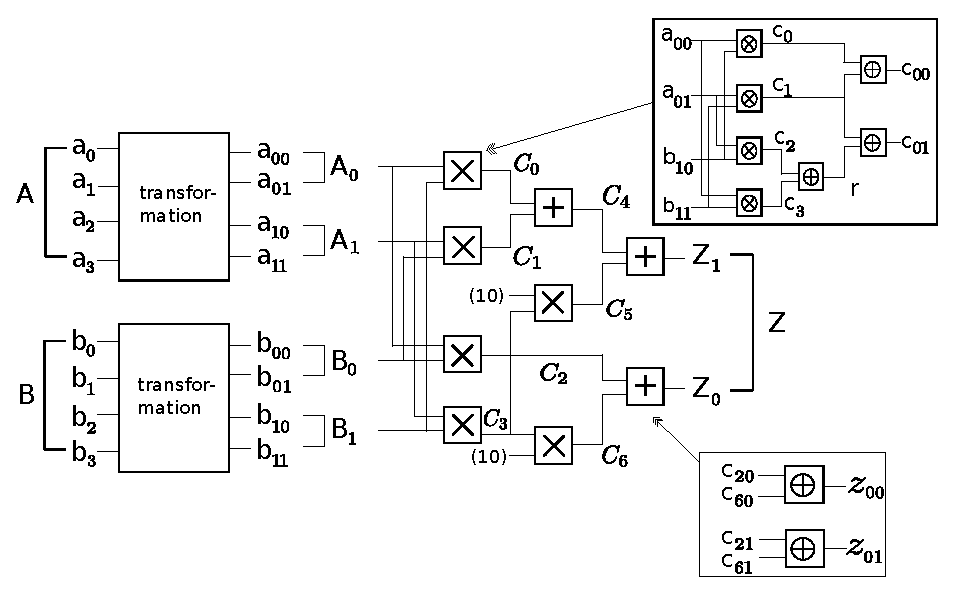
\includegraphics[width=\linewidth]{./figures/compMineSmall.eps}
%% }
%% \caption{Galois field multiplier over the composite field $\mathbb{F}_{(2^2)^2}$}
%% \label{fig:mas22}
%% \end{figure}

%% \begin{Example}
%% Consider the $4$-bit Mastrovito multiplier circuit over $\F_{2^4}$
%% shown in Figure \ref{fig:mas4}, where $A$ and $B$ are the $4$-bit 
%% word-level inputs and $\{a_0,a_1,a_2,a_3,b_0,b_1,b_2,b_3\}$ are
%% primary inputs, thus
%% \begin{eqnarray}
%% A=a_0+a_1\alpha+a_2\alpha^2+a_3\alpha^3 \nonumber \\
%% B=b_0+b_1\alpha+B_2\alpha^2+B_3\alpha^3 \nonumber
%% \end{eqnarray}

%% Since the field $\F_{2^4}$ can be decomposed as $\F_{(2^2)^2}$, 
%% this multiplier can be constructed as a composite field multiplier
%% over $\F_{(2^2)^2}$ with the base field $\F_{2^2}$.
%% Such a multiplier is shown Figure \ref{fig:mas22} and
%% is represented as follows:
%% \begin{eqnarray}
%% A = A_0+A_1\gamma \nonumber \\
%% B = B_0+B_1\gamma \nonumber \\
%% A_0=a_{00}+a_{01} \cdot \beta \nonumber \\
%% A_1=a_{10}+a_{11} \cdot \beta \nonumber \\
%% B_0=b_{00}+b_{01} \cdot \beta \nonumber \\
%% B_1=b_{10}+b_{11} \cdot \beta \nonumber
%% \end{eqnarray}
%% where $A_0,A_1,B_0,B_1$ are the $2$-bit inputs $\in \F_{2^2}$
%% composed of $a_{00},a_{01},a_{10},a_{11},b_{00},b_{01},b_{10},b_{11}$, 
%% which are the bit-level inputs to the composite field multiplier
%% derived from the transformation of $\{a_0,a_1,a_2,a_3,b_0,b_1,b_2,b_3\}$.
%% Correspondingly, each block in Figure \ref{fig:mas22}
%% internally represents a $2$-bit operation: $\times$ represents $2$-bit
%% {\it multiplication} and $+$ represents $2$-bit {\it addition} over
%% the ground field.
%% \end{Example}

%\afterpage{%
%    \clearpage% Flush earlier floats (otherwise order might not be correct)
%    \thispagestyle{empty}% empty page style (?)
%	\global\pdfpageattr\expandafter{\the\pdfpageattr/Rotate 90}
%    \begin{landscape}% Landscape page
     
%\begin{sidewaysfigure}
%\begin{figure}[h!]
%\centerline{
%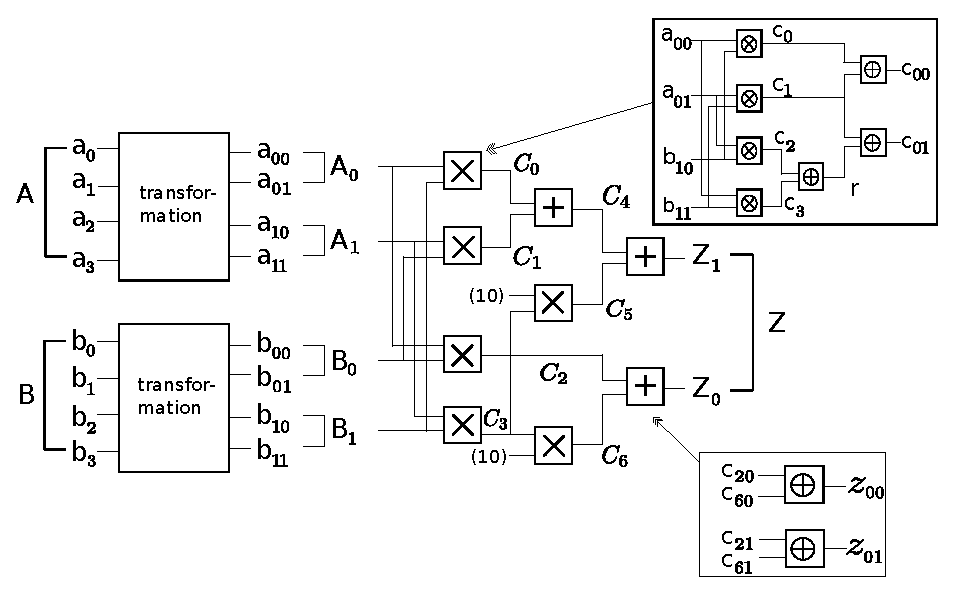
\includegraphics[width=.9\linewidth]{./figures/compMineSmall.eps}
%}
%\caption{Mastrovito multiplier over the composite field $\mathbb{F}_{(2^2)^2}$}
%\label{fig:mas22}
%\end{figure}
%\end{sidewaysfigure}
%  
%    \end{landscape}
%    \clearpage% Flush page
%	\global\pdfpageattr\expandafter{\the\pdfpageattr/Rotate 0}
%}

%%%%%%%%%%%%%%%%%%%%%%%%%%%%%%%%%%%%%%%%%%%
\subsection{Applications to Elliptic Curve Cryptography}
Elliptic Curve Cryptography (ECC) is one of the most influential applications 
of Galois fields.
ECC is an approach to public-key (or asymmetric-key) cryptography based on the 
algebraic structure of elliptic curves over Galois fields. Due to the complex 
nature of these curves, key sizes in ECC can be smaller than other public-key
cryptography techniques while providing the same level of security \cite{ecc:book}.
The main operations of encryption, decryption and authentication in ECC 
rely on {\it point multiplications}.


Point multiplication involves a series of addition and doubling of points on the 
elliptic curve.
A drawback of traditional point multiplication is that each point addition and 
doubling require a multiplicative inverse operation over Galois fields, 
the computation of which is costly.
Modern methods, however, represent the points in 
projective coordinate systems \cite{ecc:software},
which has eliminated the need for a multiplicative inverse operation by replacing it 
with addition and multiplication operations over Galois fields.
This has increased the efficiency of point multiplication operations, but it has also
increased the need for fast, custom hardware designs of Galois field arithmetic.

In-depth analysis of elliptic curve theory is beyond the scope of this 
dissertation. Instead, we will look at some examples of point addition and point doubling to
give a general idea of the operations involved in ECC and how they apply to Galois 
field arithmetic. Our experiments use custom Galois field arithmetic designs based 
on L$\acute{o}$pez-Dahab (LD) coordinate system \cite{eccld}, so these examples will
use the same coordinate system. 

\begin{figure}[h]
	\begin{center}
	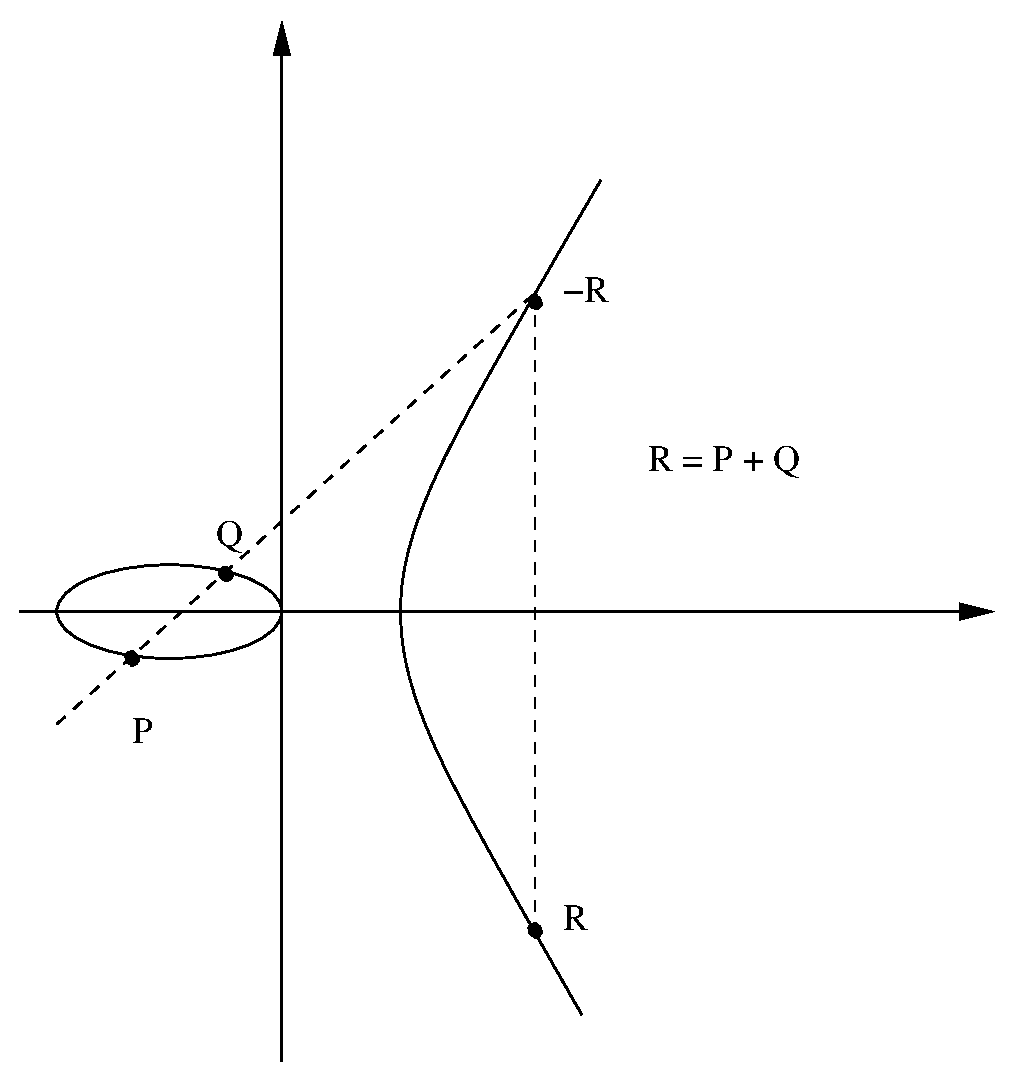
\includegraphics[scale=0.50]{figures/ecc}
	\end{center}
	\caption{Point addition over an Elliptic Curve (R=P+Q)}
	\label{fig:ecc}
\end{figure}

\begin{Example}
Consider point addition in a LD projective coordinate system, 
as seen in Fig. \ref{fig:ecc}. 

Given an elliptic curve: $Y^2 + XYZ = X^3Z + aX^2Z^2 + bZ^4$ over $\mathbb{F}_{2^k}$, 
where $X,Y,Z$ are $k$-bit vectors
that are elements in $\mathbb{F}_{2^k}$ and similarly, 
$a, b$ are constants from the field. 
Let $P + Q = R$ represent point addition over the elliptic curve.
$P=(X_1, Y_1, Z_1)$ and $Q=(X_2, Y_2, 1)$ are given.
Then $R=(X_3, Y_3, Z_3)$ can be computed as follows:

\begin{align*}
A &= Y_2 \cdot Z_1^2 + Y_1 \\
B &= X_2 \cdot Z_1 + X_1 \\
C &= Z_1 \cdot B \\
D &= B^2 \cdot(C + a Z_1^2) \\
Z_3 &= C^2 \\
E &= A \cdot C  \\
X_3 &= A^2 + D + E  \\
F &= X_3 + X_2 \cdot Z_3 \\
G &= X_3 + Y_2\cdot Z_3 \\
Y_3 &= E\cdot F + Z_3 \cdot G \\
\end{align*}
\end{Example}

\begin{Example}
Consider point doubling in a LD projective coordinate system. 
Given an elliptic curve: $Y^2 + XYZ = X^3Z + aX^2Z^2 + bZ^4$. 
Let 2($X_1$, $Y_1$, $Z_1$) = ($X_3$, $Y_3$, $Z_3$), then

\begin{align*}
X_3 &= X_1^4 + b \cdot Z_1^4  \\
Z_3 &= X_1^2 \cdot Z_1^2 \\
Y_3 &= b Z_1^4 \cdot Z_3 + X_3 \cdot (aZ_3 + Y_1^2 + bZ_1^4 ) \\
\end{align*}
\end{Example}

In the above examples, polynomial multiplication and squaring operations can be 
implemented in hardware using Montgomery reductions over Galois fields $\mathbb{F}_
{2^k}$. In practical applications, the field size $k$ of $\mathbb{F}_{2^k}$ is $163$,
or larger. However, there are no word-level 
abstraction techniques applicable to circuits of such size, so hardware 
implementations of Galois field arithmetic circuits 
cannot benefit from the many advantages of abstraction.
Thus, we propose a computer-algebra approach to word-level polynomial abstractions 
of Galois field arithmetic circuits.
Recent computer-algebra formal verification techniques \cite{lv:phd} 
have been able to verify these circuits up to $163$ bits. 
We propose an application of our abstraction approach to improve these techniques. 
These improvements allow us to perform formal verification of these
circuits up to $571$ bits. These proposals are described in detail in 
subsequent chapters.

\chapter{Computer Algebra Fundamentals} \label{ch:ideals}
This chapter reviews fundamental concepts of commutative and 
computer algebra which are used in this work. 
Specifically, this chapter covers monomial ordering, polynomial ideals and 
varieties, and the computation of \Grobner bases.
It also overviews elimination theory as well as Hilbert's Nullstellensatz 
theorems and how
they apply to Galois fields. The results of these theorems are used in polynomial
abstraction and formal verification of Galois field circuits and 
are discussed 
in subsequent chapters. The material of this chapter is
mostly referred from the textbooks \cite{ideals:book} \cite{gb_book} and 
previous work by {\it Lv} \cite{lv:phd}. 

\section{Monomials, Polynomials, and Term Orderings}

\begin{Definition} \label{def:mono}
A {\bf monomial} in variables $x_1,x_2,\cdots,x_d$ is a product of the form:
\begin{equation}
x_1^{{\alpha}_1} \cdot x_2^{{\alpha}_2} \cdot \cdots x_d^{{\alpha}_d},
\end{equation}
where $\alpha_i \ge 0, i\in\{1,\cdots,d\}$. 
The total degree of the monomial is $\alpha_{1}+\cdots+\alpha_{d}$.
\end{Definition} 

Thus, $x^2\cdot y$ is a monomial in variables $x,y$ with total degree $3$.
For simplicity, we will henceforth denote a 
monomial $x_1^{{\alpha}_1} \cdot x_2^
{{\alpha}_2} \cdot \cdots x_d^{{\alpha}_d}$ as $x^{\alpha}$, 
where $\alpha=({\alpha}_1,\cdots,{\alpha}_d)$ is a vector size $d$ of 
integers $\ge 0$, i.e., $\alpha \in \mathbb{Z}_{\ge 0}^{d}$. In the

\begin{Definition}
A {\bf multivariate polynomial} $f$ in variables $x_1, x_2, \ldots, x_d$ 
with coefficients in any given field $\K$ is a finite linear 
combination of monomials with coefficients in $\K$: 
\begin{equation}
	f=\sum_{\alpha}a_{\alpha}\cdot x^{\alpha}, ~~a_{\alpha}\in \K \nonumber
\end{equation}

The set of all polynomials in $x_1, x_2, \ldots, x_d$ with coefficients in 
field $\K$ is denoted by $\K[x_1, x_2, \ldots, x_d]$. 
Thus, $f \in \K[x_1, x_2, \ldots, x_d]$

\begin{enumerate}
\item We refer to the constant $a_{\alpha} \in \K$ as the 
{\bf coefficient} of the monomial $a_{\alpha} x^{\alpha}$.
\item If $a_{\alpha} \neq 0$, we call $a_{\alpha} x^{\alpha}$ a term of $f$.
\end{enumerate}
\end{Definition}

As an example, $2x^2+y$ is a polynomial with two terms $2x^2$ and $y$, with 
$2$ and $1$ as coefficients respectively. 
In contrast, $x+y^{-1}$ is not a polynomial because the exponent of $y$ is 
less than $0$.

Since a polynomial is a sum of its terms,
these terms have to be arranged unambiguously so that they can be 
manipulated in a consistent manner.
Therefore, we need to establish a concept of 
{\bf term ordering} (also called monomial ordering).
A term ordering, represented by $>$, defines how
terms in a polynomial are ordered.
%%%%%%%%%%%%%%%%%%%   monomial    Ordering   %%%%%%%%%%%%%%%%%%%%%%%%%%%%
\begin{Definition}
Let $\mathbb{T}^{d}=\{x^{\alpha}: \alpha\in \mathbb{Z}_{\ge 0}^{d}\}$ be the set of all monomials in $x_{1},\dots,x_{d}$.
A {\bf monomial order} $>$ on $\mathbb{T}^{d}$ is a total well-ordering satisfying:
\begin{itemize}
        \item For all $x^{\alpha}, x^{\beta} \in \mathbb{T}^{d}$, $x^{\alpha}$ and $x^{\beta}$ are comparable
	\item For any $x^{\alpha} \in \mathbb{T}^{d}$, $x^{\alpha}>1$
	\item For all $x^{\alpha}, x^{\beta}, x^{\gamma} \in \mathbb{T}^{d}$, $x^{\alpha}>x^{\beta} \Rightarrow x^{\alpha} \cdot x^{\gamma}> x^{\beta} \cdot x^{\gamma}$
\end{itemize}
\end{Definition}

Term-orderings are totally ordered, i.e. anti-symmetric with constant terms
last in the ordering.
A total-order ensures that there is no ambiguity with respect to where a 
term is found in the term-ordering.  Total orderings for monomials come in 
different forms, notably 
lexicographic orderings (lex), and its variants: degree-lexicographic ordering (deglex) 
and reverse degree-lexicographic ordering (degrevlex).

A {\bf lexicographic ordering} (lex) is a total-ordering $>$ such that 
variables in the terms are lexicographically ordered, i.e. simply based on 
when the variables appear in the ordering.
Higher variable-degrees take 
precedence over lower degrees for equivalent variables (e.g. $a^3 > a^2$ due to $a \cdot a \cdot a > a \cdot a \cdot 1$).
\begin{Definition}
{\bf Lexicographic order:} Let $x_1 > x_2 > \dots > x_d$
lexicographically. Also let $\alpha = (\alpha_1, \dots, \alpha_d);
~\beta = (\beta_1, \dots, \beta_d) \in \mathbb{Z}^d_{\geq 0}$. Then we
have: 
\begin{equation}
x^{\alpha} > x^{\beta} \iff 
\begin{cases}
& \text{Starting  from the  left, the first co-ordinates of $\alpha_i, \beta_i$} \\
& \text{that are different satisfy $\alpha_i > \beta_i$}

\end{cases}
\end{equation}
\end{Definition}

A {\bf degree-lexicographic ordering} (deglex) is a total-ordering $>$ such 
that the total degree of a term takes precedence over the lexicographic 
ordering.  
A {\bf degree-reverse-lexicographic ordering} (degrevlex) is the same as a
deglex ordering, however terms are lexed in reverse.

\begin{Definition}
{\bf Degree Lexicographic order:} Let $x_1 > x_2 > \dots > x_d$
lexicographically. Also let $\alpha = (\alpha_1, \dots, \alpha_d);
~\beta = (\beta_1, \dots, \beta_d) \in \mathbb{Z}^d_{\geq 0}$. Then we
have: 
\begin{equation}
x^{\alpha} > x^{\beta} \iff 
\begin{cases}
\sum_{i=1}^{d}\alpha_i > \sum_{i=1}^{d} \beta_i & \text{ or }\\
\sum_{i=1}^{d}\alpha_i = \sum_{i=1}^{d} \beta_i  \text{ and }
x^{\alpha} > x^{\beta} & \text{w.r.t. lex order}
\end{cases}
\end{equation}
\end{Definition}


\begin{Definition}
{\bf Degree Reverse Lexicographic order:} Let $x_1 > x_2 > \dots > x_d$
lexicographically. Also let $\alpha = (\alpha_1, \dots, \alpha_d);
~\beta = (\beta_1, \dots, \beta_d) \in \mathbb{Z}^d_{\geq 0}$. Then we
have: 
\begin{equation}
x^{\alpha} > x^{\beta} \iff 
\begin{cases}
\sum_{i=1}^{d}\alpha_i > \sum_{i=1}^{d} \beta_i  \text{ or }\\
\sum_{i=1}^{d}\alpha_i = \sum_{i=1}^{d} \beta_i  \text{ and the first co-ordinates}\\
\text{$\alpha_i, \beta_i$ from the right, which are different, satisfy $\alpha_i < \beta_i$}
\end{cases}
\end{equation}

\end{Definition}

Applying these term orderings, we have the following relations, 
where $a > b > c$.

\begin{eqnarray}
    \eqntext{lex:}  
    a^2b > a^2 > abc > ab > ac^2 > ac > b^2c > b^2 > bc^3 > 1 
    \label{ex:ordering:lex}\\
    \eqntext{deglex:} 
    bc^3 > a^2b > abc > ac^2 > b^2c > a^2 > ab >
    ac > b^2 > 1
    \label{ex:ordering:deglex}\\
    \eqntext{degrevlex:}  
    bc^3 > a^2b > abc > b^2c > ac^2 > a^2 > ab >
    b^2 > ac > 1
    \label{ex:ordering:degrevlex}
\end{eqnarray}

The difference between the {\it lex} and two {\it deg-} orderings is
obvious, while the difference between the two degree-based orderings can be
seen by considering from which direction the term is lexed, e.g. $a\cdot c\cdot c > b\cdot b\cdot c$ (deglex, left-to-right)
versus $b\cdot b\cdot c > a \cdot c\cdot c$ (degrevlex, right-to-left). 

\begin{Example}
Let $f = 2x^2yz + 3xy^3 - 2x^3$. The effects of different term orderings on 
$f$ are:
\begin{itemize}
\item lex $x> y> z$: $f = -2x^3 + 2x^2yz + 3xy^3$
\item deglex $x>y>z$:  $f = 2x^2yz + 3xy^3 -2x^3$
\item degrevlex $x>y>z$: $f = 3xy^3 + 2x^2yz - 2x^3$
\end{itemize}
\end{Example}

%Based on the {\it monomial ordering}, we have the following concepts:

\begin{Definition}
The {\bf leading term} is the first term in a term-ordered polynomial.
Likewise, the {\bf leading coefficient} is the coefficient of
the leading term. 
Finally, a {\bf leading monomial} is the leading term 
lacking the coefficient.  We use the following notation:
\begin{eqnarray}
     lt(f)&& \text{--- Leading Term} \\
     lc(f)&& \text{--- Leading Coefficient} \\
     lm(f)&& \text{--- Leading Monomial} \\
     tail(f)&& f - lt(f)
\end{eqnarray}
\end{Definition}

\begin{Example}
\begin{eqnarray}
     f      &=& 3a^2b + 2ab + 4bc \\
     lt(f)  &=& 3a^2b \\
     lc(f)  &=& 3 \\
     lm(f)  &=& a^2b \\
     tail(f) &=& 2ab+4bc
\end{eqnarray}
\end{Example}

{\bf Polynomial division} is an operation over polynomials that is dependent on
the imposed monomial ordering. Dividing a polynomial $f$ by another polynomial
$g$ cancels the leading term of $f$ to derive a new polynomial. 

\begin{Definition}
Let $\K$ be a field and let $f, g \in \K[x_1, x_2, \ldots, x_d]$ be polynomials
over the field. {\bf Polynomial division} of $f$ by $g$ is computes following:
\begin{equation}
f-\frac{lt(f)}{lt(g)}\cdot g
\end{equation}
This polynomial division is denoted
\begin{equation}
f\xrightarrow{g} r
\end{equation}
where $r$ is the resulting polynomial of the division.
If $\frac{lt(f)}{lt(g)}$ is non-zero, then $f$ is considered divisible by $g$, 
i.e. $g \mid f$.
\end{Definition}
Notice that if $g \nmid f$, that is if $f$ is not divisible by $g$,
then the division operation gives $r = f$.
\begin{Example}
Over $\R[x,y,z]$, set the lex term order $x > y > z$.
Let $f = -2x^3 + 2x^2yz + 3xy^3$ and $g = x^2+yz$.
\begin{equation}
\frac{lt(f)}{lt(g)} = \frac{-2x^3}{x^2} = -2x
\end{equation}
Since $\frac{lt(f)}{lt(g)}$ is non-zero $g|f$. The division, $f\xrightarrow{g} r$, 
is computed as:
\begin{eqnarray}
r &=& f-\frac{lt(f)}{lt(g)}\cdot g = -2x^3 + 2x^2yz + 3xy^3 - (-2x \cdot (x^2+yz)) \nonumber \\
&=& -2x^3 + 2x^2yz + 3xy^3 - (-2x^3-2xyz) = 2x^2yz + 3xy^3 + 2xyz
\end{eqnarray}
Notice that the division cancels the leading term of $f$.
\end{Example}

\section{Varieties and Ideals}
%%%%%%%%%%%%%%%%%%%%%%%%%%%%%%%%%%%%%%%%%%%%%%%%%%%%%%%%%%%%%%%%%%%%%%%%%%%%
%%%%%%%%%%%%%%%%%%%%%  variety %%%%%%%%%%%%%%%%%%%%%%%%%%%%%%%%%%%%%%%%%%
In computer-algebra based formal verification,
it is often necessary to analyze the presence 
or absence of solutions to a given system of constraints.
In our applications, these constraints are polynomials and their solutions 
are modeled as {\bf varieties}.

\begin{Definition}
Let $\K$ be a field, and let $f_1, \ldots, f_s 
\in \K[x_1, x_2, \ldots, x_d]$. 
We call $V(f_1, \dots, f_s)$ the {\bf affine variety} 
defined by $f_1, \dots, f_s$ as:
\begin{equation}
V(f_1, \ldots, f_s)= \{(a_1, \ldots, a_{d})\in \K^d:f_i(a_1, \ldots, a_d)=0, \forall{i},1\le i \le s\}
\end{equation}
\end{Definition}

$V(f_1, \dots, f_s)\in \K^d$ is {\bf the set of all solutions} in $\K^d$ 
of the system of equations: 
$f_1(x_1,\ldots,x_d)=\dots=f_s(x_1,\dots,x_d)=0$. 

\begin{Example}
Given $\mathbb{R}\left[x,y\right]$, $V(x^2+y^2)$ is the set of all elements
that satisfy $x^2+y^2=0$ over $\mathbb{R}^2$. So $V(x^2+y^2)=\{(0,0)\}$. 
Similarly, in $\mathbb{R}\left[x,y\right]$, $V(x^2+y^2-1)=\{all\  points\  on\ the\ circle: x^2+y^2-1=0\}$.
Note that varieties depend on which field we are operating on. 
For the same polynomial $x^2+1$, we have:
\begin{itemize}
\item In $\mathbb{R}[x]$, $V(x^2+1)=\emptyset$.
\item In $\mathbb{C}[x]$, $V(x^2+1)=\{(\pm i)\}$.
\end{itemize}
\end{Example}

The above example shows the variety can be infinite, finite (non-empty set) 
or empty. It is interesting to note that since we will be operating over
finite fields $\F_{q}$, and any finite set of points is a variety. Likewise,
any variety over $\F_{q}$ is finite (or empty).
Consider the points $\{(a_1,\dots, a_d): a_1, \dots, a_d \in \F_q\}$
in $\F_q^d$. Any single point is a variety of some polynomial system:
e.g. $(a_1,\dots, a_d)$ is a variety of $x_1-a_1 = x_2 - a_2 = \dots =
x_d-a_d=0$. {\bf Finite unions} and {\bf finite  intersections} of
varieties are also varieties. 

\begin{Example}
Let $U = V(f_1, \dots, f_s)$ and $W =
V(g_1, \dots, g_t)$ in $\F_{q}$. Then:  
\begin{itemize}
\item $U \cap W = V(f_1, \dots, f_s, g_1, \dots, g_t)$
\item $U \cup W = V(f_i g_j: 1 \leq i \leq s, 1 \leq j \leq t)$
\end{itemize}
\end{Example}

One important distinction we need to make about varieties is that a
variety depends not just on the given system of polynomial 
equations, but rather on the {\bf ideal} generated by the polynomials.

%%%%%%%%%%%%%%%%%%%%%  ideal %%%%%%%%%%%%%%%%%%%%%%%%%%%%%%%%%%%%%%%%%%
\begin{Definition} 
A subset $I \subset \K[x_1, x_2, \ldots, x_d]$ is an {
\bf ideal} if it satisfies:
\begin{itemize}
\item $0 \in I$
\item $I$ is closed under addition: $x, y \in I \Rightarrow x+y \in I$
\item If $x \in \K[x_1, x_2, \ldots, x_d]$ and $y \in I$, then $x\cdot y \in I$ and $y\cdot x \in  I$.
\end{itemize}
\end{Definition}

An ideal is generated by its {\it basis} or {\it generators}.

%%%%%%%%%%%%%%%%%%%%%  ideal basis%%%%%%%%%%%%%%%%%%%%%%%%%%%%%%%%%%
\begin{Definition}
Let $f_1, f_2, \ldots, f_s$ be 
polynomials of the ring $\K[x_1, x_2, \ldots, x_d]$. 
Let $I$ be an ideal generated by $f_1, f_2, \ldots, f_s$. Then:
\begin{equation}
I = \langle f_1,\dots,f_s \rangle=\{h_1 f_1 + h_2 f_2 + \ldots + h_s f_s : h_1,\dots,h_s\in\K[x_1, \dots, x_d]\} \nonumber
\end{equation}
then, $f_1, \ldots, f_s$ are called the {\bf basis (or generators)} of the 
ideal $I$ and correspondingly $I$ is denoted as $I = \langle f_1, f_2, 
\ldots, f_s \rangle$. 
\end{Definition}

\begin{Example}
The set of even integers, which is a subset of the ring of integers
$Z$, forms an ideal of $Z$. This can be seen from the following;
\begin{itemize}
\item $0$ belongs to the set of even integers.
\item The sum of two even integers $x$ and $y$ is always an even
  integer.
\item The product of any integer $x$ with an even integer $y$ is
  always an even integer.
\end{itemize}
\end{Example}

\begin{Example}
Given $\mathbb{R}\left[x,y\right]$, $I = \langle x, y \rangle$ is an 
ideal containing all polynomials generated by $x$ and $y$, 
such as $x^2+y$ and $x+x\cdot y$.
$J = \langle x^2, y^2 \rangle$ is an ideal containing all polynomials 
generated by $x^2$ and $y^2$, such as $x^2+y^3$ and $x^{10}+x^2\cdot y^2$. 
Notice that $J\subset I$ because every polynomial generated by $J$ can
be generated by $I$. 
But $I\neq J$ because $x+y$ can only be generated by $I$.
\end{Example}

The same ideal may have many different bases.
For instance, it is possible to have different sets of polynomials
$\{f_1,\dots,f_{s}\}$ and $\{g_{1},\dots,g_{t}\}$ that may generate the same 
ideal, i.e., 
$\langle f_{1},\dots,f_{s}\rangle=\langle g_{1},\dots,g_{t}\rangle$. Since 
variety depends on the ideal, these sets of polynomials have the same 
solutions.

\begin{Proposition}
If $f_1,\dots,f_{s}$ and $g_{1},\dots,g_{t}$ are bases of the same ideal 
in $\mathbb{F}[x_{1},\dots,x_{d}]$,
so that $\langle f_{1},\dots,f_{s}\rangle=\langle g_{1},\dots,g_{t}\rangle$, 
then $V(f_{1},\dots,f_{s})=V(g_{1},\dots,g_{t})$.
\end{Proposition}

\begin{Example}
	Consider the two bases $F_{1}=\{(2x^{2}+3y^{2}-11,x^{2}-y^{2}-3\}$ and $F_{2}=\{x^{2}-4,y^{2}-1\}$.
	These two bases generate the same ideal, i.e., $\langle F_{1}\rangle= \langle F_{2} \rangle$.{}
	Therefore, they represent the same variety, i.e., 
	\begin{equation}
		V(F_{1})= V( F_{2})=\{\pm 2, \pm 1\}.
	\end{equation}
\end{Example}

Ideals and their varieties are a key part of computer-algebra based formal
verification. A given hardware design can be transformed into a set
of polynomials over a field, $f_1, \ldots, f_s \in F$ 
(we showed how this is done for Galois field arithmetic 
circuits in the previous chapter).
This set of polynomials gives the system of equations:
\begin{eqnarray}
f_1 = 0 \nonumber \\
\vdots \nonumber \\
f_s = 0 \nonumber
\end{eqnarray}
Using algebra, it is possible to derive new equations from the original 
system.
The ideal $\langle f_1,\ldots, f_s \rangle$ provides a way of analyzing 
such {\it consequences} of a system of polynomials.

\begin{Example}
Given two equations in $\mathbb{R}[x,y,z]$:
\begin{eqnarray}
x=z+1 \nonumber \\
y=x^2+1 \nonumber 
\end{eqnarray}
we can eliminate $x$ to obtain a new equation:
\begin{equation}
y=(z+1)^2+1=z^2+2z+2 \nonumber 
\end{equation}
Let $f_1, f_2, h \in \mathbb{R}[x,y,z]$ be polynomials based on these 
equations:
\begin{eqnarray}
f_1 = x-z-1 &= 0 \nonumber \\
f_2 = y-x^2-1 &= 0 \nonumber \\
h   = y-z^2-2z-2 &= 0 \nonumber
\end{eqnarray}
If $I$ is the ideal generated by $f_1$ and $f_2$, i.e. 
$I=\langle f_1, f_2 \rangle$, then we find $h \in I$ as follows:
\begin{eqnarray}
g_1 = x+z+1 \nonumber \\
g_2 = 1     \nonumber \\
h = g_1\cdot f_1+g_2\cdot f_2  = y-z^2-2z-2 \nonumber
\end{eqnarray}
where $g_1, g_2 \in \mathbb{R}[x,y,z]$.
Thus, we call $h$ a {\bf member of the ideal} $I$.
\end{Example}

%\subsection{Ideals of Varieties}

Let $\mathbb{K}$ be any field and let $\mathbf{a}=(a_{1},\dots,a_{d}) \in \mathbb{K}^d$ be a point, and $f \in
\mathbb{K}[x_1,\dots, x_d]$ be a polynomial. We say that $f$ {\it vanishes} on $\mathbf{a}$ if $f(\mathbf{a}) = 0$, i.e.,
$\mathbf{a}$ is in the variety of $f$.

\begin{Definition}
For any variety $V$ of $\mathbb{K}^d$, the ideal of polynomials that vanish on $V$,
called the {\it vanishing ideal of $V$}, is defined as $I(V) = \{f\in
\mathbb{F}[x_1,\dots, x_d]: \forall \mathbf{a} \in V, f(\mathbf{a}) =
0\}$. 
\end{Definition}

\begin{Proposition}\label{pro:iofv}
	If a polynomial $f$ vanishes on a variety $V$, then $f \in I(V)$. 
\end{Proposition}

\begin{Example}
	Let ideal $J=\langle x^{2},y^{2}\rangle$. Then $V(J)=\{(0,0)\}$.
	All polynomials in $J$ will obviously agree with the solution and vanish on this variety.
	However, the polynomials $x,y$ are not in $J$ but they also vanish on this variety. 
	Therefore, $I(V(J))$ is the set of all polynomials that vanish on $V(J)$, and the polynomials
	$x,y$ are members of $I(V(J))$.
\end{Example}

\begin{Definition}\label{def:radical}
Let $J \subset \mathbb{K}[x_1,\dots, x_d]$ be an ideal. The {\it radical of $J$} is defined as $\sqrt{J} = \{f \in
\mathbb{K}[x_1,\dots, x_d]: \exists m \in \mathbb{N}, f^m \in J\}$. 
\end{Definition}

\begin{Example}
Let $J=\langle x^2,y^2\rangle \subset \mathbb{K}\left[x,y\right]$.
Note neither $x$ nor $y$ belongs to $J$, but they belong to $\sqrt J$.
Similarly, $x\cdot y \notin J$, but since $(x \cdot y)^{2}=x^{2}\cdot y^{2}\in J$, therefore,
$x\cdot y \in \sqrt J$. 
\end{Example} 

When $J = \sqrt J$, then $J$ is said to be a 
{\it radical ideal}. Moreover, $I(V)$ is a radical ideal.
By analyzing the ideal $J$, generated by a system of polynomials derived 
from a hardware design, its variety $V(J)$, and the ideal of 
polynomials that vanish over this variety, $I(V(J))$, we can reason about the 
existence of certain properties of the design. To check for the existence of 
a property, we formulate the 
property as a polynomial and then perform an {\bf ideal membership test} to 
determine if this polynomial is contained within the ideal $I(V(J))$. 
A {\bf \Grobner basis} provides a decision procedure for performing this 
test, which is described in the following section. 
A future section focuses on {\bf Hilbert's Nullstellensatz}, 
which describes the properties of the ideal of a variety, $I(V(J))$. 

%%%%%%%%%%%%%%%%%%%%	Grobner bases	%%%%%%%%%%%%%%%%%%%%%%%%%%%%%%%%%%
\section{\Grobner Bases}

As mentioned earlier, different polynomial sets may generate the same 
ideal. Some of these generating sets may be a better representation of 
the ideal, and thus provide more information and insight into the properties 
of ideal. One such ideal representation is a {\bf \Grobner basis}, which has
a number of important properties that can solve numerous polynomial 
decision questions:

\begin{itemize}
\item Presence or absence of solutions (varieties)
\item Dimension of the varieties
\item Ideal membership of a polynomial
\end{itemize} 

In essence, a \Grobner basis is a canonical representation of an ideal.
There are many equivalent definitions of \Grobner bases, so we start with 
the definition that best describes their properties:

\begin{Definition}
A set of non-zero polynomials $G=\{g_1,\dots,g_t\}$ which generate the 
ideal $I=\langle g_1,\dots,g_t\rangle$, is called a 
{\bf Gr\"obner basis} for $I$ if and only if 
for all $f \in I$ where $f \neq 0$, there exists a $g_i \in G$ such that $lm(g_i)$ divides $lm(f)$.
\begin{eqnarray}
G = \text{Gr\"obner{Basis}} (I) \iff 
\forall f \in I: f \neq 0, \exists g_i \in G: lm(g_i)\ |\ lm(f)
        \label{eqn:groebnermin}
    \end{eqnarray}
    
\end{Definition}

The foundation for computing the \Grobner basis of an ideal was laid out 
by Buchberger\cite{buchberger_thesis}.
Given a set of polynomials $F=\{f_{1},\dots,f_{s}\}$ that generate ideal $I=
\langle f_{1},\dots,f_{s} \rangle$, 
Buchberger gives an algorithm to compute a Gr\"obner basis $G=\langle g_{1},
\dots,g_{t}\rangle$. This algorithm relies on the notions of $S$-polynomials 
and polynomial reduction.

\begin{Definition}
For $f, g \in \K[x_1,\dots,x_d]$, an {\bf S-polynomial} $Spoly(f,g)$ is 
defined as:
\begin{equation}
    Spoly(f,g)=\frac{L}{lt(f)}\cdot f - \frac{L}{lt(g)}\cdot g
    \label{eqn:spoly}
\end{equation}
\begin{equation}
\text{where }L = lcm\left(lt(f), lt(g)\right) \nonumber
\end{equation}
Note $lcm$ denotes least common multiple.
\end{Definition}

\begin{Definition}
    The {\bf reduction} of a polynomial $f$, by another polynomial $g$, to
    a reduced polynomial $r$ is denoted:
    \begin{equation*}
        f\stackrel{g}{\textstyle\longrightarrow}r
    \end{equation*}
    Reduction is carried out using multivariate, polynomial long division. 
    % The long division is performed according to a term-ordering on polynomials, and the division algorithm 
    %terminates when the leading term of the divisor does not divide any 
    %other term in the dividend.
  
    For sets of polynomials, the notation 
    \begin{equation*}
    f\stackrel{F}{\textstyle\longrightarrow}_+r    
    \end{equation*}
    represents the reduced polynomial $r$ resulting from $f$ as reduced by a 
    set of non-zero polynomials $F = \{f_1,\dots,f_s\}$.  The polynomial $r$ is considered {\bf reduced} if 
    $r = 0$  or no term in $r$ is divisible  by a $lm(f_i), \forall f_i \in F$.
\end{Definition}

The reduction process $f\stackrel{F}{\textstyle\longrightarrow}_+r$, of 
dividing a polynomial $f$ by a set of polynomials of $F$, can be modeled as
repeated long-division of $f$ by each of the polynomials in $F$ until no
further reductions can be made. The result of this process is then $r$.
This reduction process is shown in Algorithm \ref{alg:polydiv}.

\begin{algorithm}[H]
\SetAlgoNoLine

 \KwIn{$f,f_{1},\dots,f_{s}$}
 \KwOut{$r,a_{1},\dots,a_{s}$, such that $f=a_{1}\cdot f_{1}+\dots+a_{s}\cdot f_{s}+r$.}
 
 $a_{1}=a_{2}=\dots=a_{s}=0$; $r=0$\;
 $p:=f$\;
 
 \While { $p \neq 0$ }
 {
	i=1\;
	divisionmark = false\;
	\While { $i\le s  $ \&\& divisionmark = false }
	{
		\eIf {$f_{i}$ can divide $p$}
		{
			$a_{i}=a_{i}+lt(p)/lt(f_{i})$\;
			$p=p-lt(p)/lt(f_{i}) \cdot f_{i}$\;
			divisionmark = true\;
		}
		{
			i=i+1\;
		}
	}
	
	\If {divisionmark = false}
	{
		$r=r+lt(p)$\;
		$p=p-lt(p)$\;
	}

 }
\caption{Polynomial Reduction}\label{alg:polydiv}
\end{algorithm}

The reduction algorithm keeps canceling the leading terms of polynomials 
until no more leading terms can be further canceled.
So the key step is $p=p-lt(p)/lt(f_{i}) \cdot f_{i}$, as the following 
example shows.
\begin{Example}
Given $f = y^{2}-x$ and $f_{1} = y - x$ in $\mathbb{Q}[x,y]$ with $deglex$: 
$y>x$, perform $f\stackrel{f_1}{\textstyle\longrightarrow}_+r$:

\begin{enumerate}
\item $f=y^{2}-x$, $f/f_{1}=f-lt(f)/lt(f_{1}) \cdot f_{1}=y^{2}-x-(y^{2} /y) \cdot (y-x)=y\cdot x-x$
\item $f=y\cdot x-x$, $f/f_{1}=f-lt(f)/lt(f_{1}) \cdot f_{1}=(y\cdot x-x)/f_{1}=x^{2}-x$
\item $f=x^{2}-x$, no more operations possible, so $r=x^{2}-x$
\end{enumerate}
\end{Example}

With the notions of $S$-polynomials and polynomial reduction in place,
we can now present Buchberger's Algorithm 
for computing Gr\"obner bases \cite{buchberger_thesis}. Note that a fixed 
monomial (term) ordering is required for a \Grobner basis 
computation to ensure that polynomials are manipulated in a consistent 
manner.

\begin{algorithm}[H]
\SetAlgoNoLine
 \KwIn{$F = \{f_1, \dots, f_s\}$, such that $I=\langle f_1, \dots, f_s\rangle$}, and term order $>$
 \KwOut{$G = \{g_1,\dots ,g_t\}$, a Gr\"{o}bner basis of $I$ }
  $G:= F$\;
  \Repeat{$G = G'$}
  {
  	$G' := G$\;
  	\For{ each pair $\{f_{i}, f_{j}\}, i \neq j$ in $G'$} 
	{
		$Spoly(f_{i}, f_{j}) \stackrel{G'}{\textstyle\longrightarrow}_+r$ \;
		\If{$r \neq 0$}
		{
			$G:= G \cup \{r\}$ \;
		}
	}
   }
\caption {Buchberger's Algorithm}\label{alg:gb}
\end{algorithm}

Buchberger's algorithm takes pairs of polynomials ($f_{i}, f_{j}$) in 
the basis $G$ and combines them into ``$S$-polynomials'' 
($Spoly(f_{i}, f_{j})$) to cancel leading terms. The $S$-polynomial is then 
reduced (divided) by all elements of $G$ to a remainder $r$, denoted as  
$Spoly(f_{i}, f_{j}) \stackrel{G}{\textstyle\longrightarrow}_+r$. This
process is repeated for all unique pairs of polynomials, including
those created by newly added elements, until no new polynomials are
generated; ultimately constructing the \Grobner basis.
\begin{Example}\label{exp:gbsimple}
Consider the ideal $I \subset \mathbb{Q}[x, y]$, $I = \langle f_1, f_2 
\rangle$, where $f_1 = yx - y, ~f_2 = y^2 - x$. 
Assume a degree-lexicographic term ordering with $y > x$ is imposed. 

First, we need to compute $Spoly(f_{1},f_{2})=x\cdot f_{2}-y\cdot f_{1}=y^{2}-x^{2}$.
Then we conduct a polynomial reduction 
$y^{2}-x^{2}\stackrel{f_{2}}{\textstyle\longrightarrow}x^{2}-x \stackrel{f_{1}}{\textstyle\longrightarrow}x^{2}-x$.
Let $f_{3}=x^{2}-x$. Then $G$ is updated as $\{f_{1},f_{2},f_{3}\}$. Next we compute $Spoly(f_{1},f_{3})=0$. So there
is no new polynomial generated. Similarly, we compute $Spoly(f_{2},f_{3})=x\cdot y^{2}-x^{3}$, followed by 
$x\cdot y^{2}-x^{3}\stackrel{f_{1}}{\textstyle\longrightarrow}y^{2}-x^{3} \stackrel{f_{2}}{\textstyle\longrightarrow}x-x^{3}
\stackrel{f_{2}}{\textstyle\longrightarrow}0$. Again, no polynomial is generated. Finally, $G=\{f_{1,}f_{2},f_{3}\}$.

\end{Example}

When computing a \Grobner basis, it's important to note that if $lt(f_i)$ 
and $lt(f_j)$ have no common variables, the S-poly reduction step in 
Buchberger's algorithm,
$Spoly(f_{i}, f_{j}) \stackrel{G'}{\textstyle\longrightarrow}_+r$,
will produce $r=0$.

\begin{Proof}
If $lt(f)$ and $lt(g)$ have no common variables,  
$L=lcm(lt(f),lt(g))=lt(f)\cdot lt(g)$. Then: 
\begin{equation}
    Spoly(f,g)=\frac{L}{lt(f)}\cdot f - \frac{L}{lt(g)}\cdot g=
\frac{lt(f)\cdot lt(g)}{lt(f)}\cdot f - \frac{lt(f)\cdot lt(g)}{lt(g)}\cdot g
= lt(g)\cdot f - lt(f)\cdot g \nonumber
\end{equation}
Thus, every monomial in $Spoly(f, g)$ is divisible by either $lt(f)$ 
or $lt(g)$, so computing 
$Spoly(f, g) \stackrel{f,g}{\textstyle\longrightarrow}_+r$ will give $r=0$.
\end{Proof}

As mentioned previously, a \Grobner basis gives a decision procedure to test 
for polynomial membership in an ideal. This is explained in the following 
Theorem.
    
\begin{Theorem}\label{the:membership}
	{\bf Ideal Membership Test}
 Let $G = \{g_1,\cdots,g_t \}$ be a Gr\"obner basis for an ideal $I \subset \mathbb{K}[x_1,\cdots,x_d ]$
	and let $f \in \mathbb{K}[x_{1},\dots, x_{d}]$. Then $f \in I$ if and only if the remainder on division of $f$ by
	$G$ is zero.
\end{Theorem}
In other words, 
\begin{equation}
f \in I \iff f \stackrel{G}{\textstyle\longrightarrow}_+0
\end{equation}

\begin{Example}
Consider Example \ref{exp:gbsimple}. Let $f = y^2x - x$ be another
polynomial. Note that $f = yf_1 + f_2$, so $f \in I$. If we divide $f$
by $f_1$ first and then by $f_2$, we will obtain a zero
remainder. However, since the set $\{f_1, f_2\}$ is not a Gr\"{o}bner
basis, we find that the reduction $f
\stackrel{f_2}{\textstyle\longrightarrow} x^2 - x
\stackrel{f_1}{\textstyle\longrightarrow} x^2 - x  \neq 0$;
i.e. dividing $f$ by $f_2$ first and then by $f_1$ does not lead to a
zero remainder. However,  if we compute the Gr\"{o}bner basis $G$ of
$I$, $G = \{x^2 - x, yx - y, y^2 - x\}$, dividing $f$ by polynomials
in $G$ in any order will always lead to the zero remainder. Therefore,
one can decide ideal membership unequivocally using the Gr\"{o}bner
basis. 
\end{Example}

A \Grobner basis is not a canonical representation of an ideal, but a
{\bf reduced \Grobner basis} is. To compute a reduced \Grobner basis, we
first must compute a minimal \Grobner basis.

\begin{Definition}\label{def:minigb}
A {\bf minimal Gr\"obner basis} for a polynomial ideal $I$ is a \Grobner basis $G$ for $I$ such that
	\begin{itemize}
		\item $lc(g_{i})=1,\forall g_{i}\in G$
		\item $\forall g_{i} \in G$,  $lt(g_{i}) \notin \langle lt(G-\{g_{i}\})\rangle$
	\end{itemize}
\end{Definition}
A {\bf minimal} \Grobner basis is a \Grobner basis such that all polynomials
have a coefficient of $1$ and no leading term of any element in $G$ divides 
another in $G$.
Given a \Grobner basis $G$, a minimal \Grobner basis can be
computed as follows:
\begin{enumerate}
\item Minimize every $g_i \in G$, i.e $g_i=g_i/lc(g_i)$
\item For $g_i, g_j \in G$ where $i\neq j$, remove $g_i$ from $G$ if $lt(g_i)\mid lt(g_j)$, i.e. remove every polynomial in $G$ whose leading term is divisible by the leading term of some other polynomial in $G$.
\end{enumerate}

A minimal Gr\"obner basis can then be further reduced.
\begin{Definition}
	A {\bf reduced Gr\"obner basis} for a polynomial ideal $I$ is a Gr\"obner basis $G=\{g_{1},\dots,g_{t}\}$ such that:
	\begin{itemize}
		\item $lc(g_{i})=1,\forall g_{i}\in G$
		\item $\forall g_{i} \in G$, no monomial of $g_{i}$ lies in $\langle lt(G-\{g_{i}\})\rangle$
	\end{itemize}
\end{Definition}
$G$ is a reduced Gr\"obner basis when no monomial of any element in $G$ 
divides the leading term of another element. 
This reduction is achieved as follows:

\begin{Definition}
Let $H = \{h_1, \ldots, h_t\}$ be a minimal Gr\"obner basis.  Apply
the following reduction process: 
\begin{itemize}
\item $h_1 \stackrel{G_1}{\textstyle\longrightarrow}_+ g_1$, where
  $g_1$ is reduced w.r.t. $G_1 = \{h_2, \ldots, h_t\}$

\item $h_2 \stackrel{G_2}{\textstyle\longrightarrow}_+ g_2$, where
  $g_2$ is reduced w.r.t. $G_2 = \{g_1, h_3, \ldots, h_t\}$
\item $h_3 \stackrel{G_3}{\textstyle\longrightarrow}_+ g_3$, where
  $g_3$ is reduced w.r.t. $G_3 = \{g_1, g_2, h_4, \ldots, h_t\}$

\hspace{0.25in} $\vdots$
\vspace{0.1in}
\item $h_t \stackrel{G_t}{\textstyle\longrightarrow}_+ g_t$, where
  $g_t$ is reduced w.r.t. $G_t = \{g_1, g_2, g_3, \ldots, g_{t-1}\}$
\end{itemize}
Then $G = \{g_1, \ldots, g_t\}$ is a {\bf reduced Gr\"obner basis.}
\end{Definition}


Subject to the given term order $>$, such a reduced Gr\"obner
  basis $G = \{g_1, \dots, g_t\}$ is a {\bf unique canonical
    representation of the ideal}, as 
given by Proposition \ref{pro:unique} below.


\begin{Proposition}\label{pro:unique} \cite{gb_book} 
Let $I \neq \{0\}$ be a polynomial ideal. Then, for a given monomial ordering, $I$ has a unique reduced Gr\"obner basis.
\end{Proposition}

\Grobner basis computation depends on the $Spoly$ computation, which in turn 
depends on the leading terms of polynomials. Thus, different monomial 
orderings can result in different \Grobner basis computations for the 
same ideal. Computation using a degrevlex ordering tends to be least 
difficult, while lex ordering tends to be computationally complex. However, 
lex ordering used in the computation of \Grobner basis is an {\bf elimination
ordering}; that is, the polynomials contained in the resulting \Grobner basis
have continuously eliminated variables in the ordering. This is the topic of 
elimination theory, which is described in the following section.

\section{Elimination Theory}

Elimination theory uses {\bf elimination ordering} 
to systematically eliminate variables from a system of polynomial
equations.

\begin{Definition}
Let $I$ be an ideal in  $\K[x_1,\dots,x_k]$. The $i$-th 
{\bf elimination ideal} $I_i$ is the ideal of $\K[x_{i+1},\dots,x_k]$ defined
by
\begin{equation}
I_k = I \cap \K[x_{i+1},\dots,x_k]
\end{equation}
\end{Definition}

The elimination ideal $I_i$ has eliminated all the variables 
$x_1,\dots,x_i$, i.e. it only contains polynomials with variables in
$x_{i+1},\dots,x_k$. 
We can generate elimination ideals by computing
\Grobner bases using elimination orderings. 

\begin{Theorem}
$\left[\bf{Elimination\  Theorem}\right]$
Let $I$ be an ideal in $\K[x_1,\dots,x_k]$ and let $G$ be the \Grobner 
basis of $I$ with respect to the lex order (elimination order) 
$x_1>x_2>\dots>x_k$. Then, for every $0\leq i\leq k$,
\begin{equation}
G_k=G\cap \K[x_{i+1},\dots,x_k]
\end{equation}
is a \Grobner basis of the $i$-th elimination ideal $I_i$.
\label{thm:elimth}
\end{Theorem}

This can be better visualized using the following example.

\begin{Example}
Given the following equations in $\R[x,y,z]$
\begin{eqnarray}
x^2+y+z&=1 \nonumber \\
x+y^2+z&=1 \nonumber \\
x+y+z^2&=1 \nonumber
\end{eqnarray}
let $I$ be the ideal generated by these equations:
\begin{equation}
I=\langle x^2+y+z-1, x+y^2+z-1, x+y+z^2-1\rangle \nonumber
\end{equation}
The \Grobner basis for $I$ with respect to lex order $x>y>z$ is 
found to be $G=\{g_1,g_2,g_3,g_4\}$ where
\begin{eqnarray}
g_1&=&x+y+z^2-1 \nonumber \\
g_2&=&y^2-y-z^2+z \nonumber \\
g_3&=&2yz^2+z^4-z^2 \nonumber \\
g_4&=&z^6-4z^4+4z^3-z^2 \nonumber
\end{eqnarray}

Notice that while $g_1$ has variables in $\R[x,y,z]$, $g_2$ and $g_3$ only 
have variables in $\R[y,z]$ and $g_4$ only has variables in $\R[z]$. Thus, 
$G_1=G\cap \R[y,z]=\{g_2,g_3,g_4\}$ and $G_2=G\cap \R[z]=\{g_4\}$

Also notice that since $g_4$ only contains variable $z$, and since $g_4=0$, 
a solution for $z$ can be obtained. This solution can then be applied to 
$g_2$ and $g_3$ to obtain solutions for $y$, and so on.
\end{Example}

Elimination theory provides the basis for our abstraction approach.


%%%%%%%%%%%%%%%%%%%%%%%%%%%%%%%%%%%%%%%%%%%%%%%%%%%%%%%%

\section{Hilbert's Nullstellensatz}

In this section, we further describe some correspondence between ideals and 
varieties in the context of algebraic geometry. The celebrated results of 
Hilbert's Nullstellensatz establish these correspondences.

%%%%%%%%%%%%%%%%%algebraically closed field%%%%%%%%%%%%%
\begin{Definition}\label{def:acf}
A field $\overline {\K}$ is an {\bf algebraically closed} field if every  
polynomial in one variable with degree at least $1$, with coefficients 
in $\overline {\K}$, has a root in $\overline {\K}$. 
\end{Definition}
In other words, any non-constant polynomial equation over 
$\overline {\K}\left[x\right]$ always has at least one root 
in $\overline {\K}$. Every field $\K$ is contained in an algebraically 
closed one $\overline {\K}$. 
For example, the field of real numbers $\mathbb{R}$ is not an algebraically closed 
field, because $x^2+1=0$ has no root in $\mathbb{R}$. 
However, $x^2+1=0$ has roots in the field of 
complex numbers $\mathbb{C}$, which is an algebraically closed field. 
In fact, $\mathbb{C}$ is the algebra closure of $\mathbb{R}$. 
Every algebraically closed field is an infinite field. 

%%%%%%%%%%%%%%%%weak nullstellensatz%%%%%%%%%%%%%
%\begin{Theorem}
%$\left[\bf{Weak\  Nullstellensatz}\right]$ Let 
%$I \subset \overline {\mathbb{K}}[x_1, x_2, \cdots, x_d]$ 
%be an ideal satisfying $V(I)=\emptyset$. 
%Then $I=\overline {\mathbb{K}}[x_1, x_2, \cdots, x_d]$, Or equivalently, 
%\begin{equation}
%V(I)=\emptyset\ \iff\ I=\overline {\mathbb{K}}[x_1, x_2, \cdots, x_d]=\langle 1 \rangle 
%\end{equation}
%\end{Theorem}
%
%\begin{Corollary}
%	Let $I=\langle f_{1},\dots,f_{s} \rangle \subset \overline {\mathbb{K}}[x_1, x_2, \cdots, x_d]$. 
%	Let $G$ be the reduced Gr\"obner basis of $I$. Then $V(I)=0 \iff G=\{1\}$.
%\end{Corollary}

%{\bf Weak Nullstellensatz} offers a way to evaluate whether or not the 
%system of multivariate polynomial equations (ideal $I$) has common solutions 
%in ${\overline {\mathbb{K}}}^d$. For this purpose, we only need to check if 
%the ideal is generated by the unit element, i.e., $1\in I$. 
%This approach can be used to evaluate the feasibility of constraints in 
%verification problems.
%%%%%%%%%%%%%%%%%%%%%%%%%strong Nullstellensatz%%%%%%%%%%%%%%%%%%%%%%%%%%%%%% 
An interesting result is one of {\bf Strong 
Nullstellensatz}.
The strong
Nullstellensatz establishes the correspondence between radical ideals
and varieties. 

\begin{Theorem}\label{thm:sns}
({\it The Strong Nullstellensatz} \cite{gb_book}) 
Let $\overline{\mathbb{K}}$ be an algebraically closed field, and let $J$
be an ideal in $\overline{\mathbb{K}}[x_1,\dots, x_d]$. 
Then we have $I(V_{\overline{\mathbb{K}}}(J)) =\sqrt{J}$. 
\end{Theorem}

%\subsection{Nullstellensatz over Galois fields}

Strong Nullstellensatz holds a special form over Galois fields $\Fq$.
Recall the notion of vanishing polynomials over Galois fields from the 
previous chapter: for every element $A \in \Fq$, $A-A^q = 0$; then the 
polynomial $x^q-x$ in $\Fq[x]$ vanishes over $\Fq$. Thus, if 
$J_0=\langle x^q-x \rangle$ is the ideal generated by the vanishing 
polynomial, $V(J_0)=\Fq$. Similarly, over $\Fq[x_1,\dots,x_d]$, $J_0$ is 
$\langle x_1^q-x_1,\dots,x_d^q-x_d \rangle$ and $V(J_0)=(F_q)^d$.


\begin{Definition}
Given two ideals, $I_1=\langle f_1, \dots,f_s \rangle$ and 
$I_2=\langle g_1,\dots g_t\rangle$, then the {\bf sum of ideals} 
$I_1+I_2=\langle f_1,\dots,f_s,g_1,\dots g_t\rangle$
\end{Definition}

\begin{Theorem}
({\it Strong Nullstellensatz over $\Fq$})
For any Galois field $\Fq$, let $J \subset \Fq[x_1,\dots,x_d]$ be any ideal 
and let $J_0 = \langle x_1^q-x_1, x_d^q-x_d \rangle$ be the ideal of all
vanishing polynomials. Let $V_{\Fq}(J)$ denote the variety of $J$ over $\Fq$.
Then, $I(V_{\Fq}(J))=J+J_0$.
\end{Theorem}

The proof is given in \cite{gao:gf-gb-ms}. Here, we provide a proof outline.

\begin{Proof}
\begin{enumerate}
\item $\sqrt{J+J_0} = J+J_0$. That is, $J+J_0$ is a radical ideal.
\item $V_{\Fq}(J)=V_{\overline{\Fq}}(J+J_0)$.
\item Due to (2), $I(V_{\Fq}(J)) = I(V_{\overline{\Fq}}(J+J_0))$. 
By Strong Nullstellensatz, this is equivalent to $\sqrt{J+J_0}$.
Finally, due to (1), this is equivalent to $J+J_0$.
\end{enumerate}
\end{Proof}

%% 
%% Using this result, Weak Nullstellensatz can be 
%% modified to be applicable over finite fields $\Fq$.
%% %%%%%%%%%%%%%%%%weak nullstellensatz in finite field%%%%%%%%%%%%%
%% \begin{Theorem}\label{wnull:ff}
%% $[\bf{Weak~Nullstellensatz~in~\Fq}]$\cite{null:1890}\\
%% Given $f_1,f_2,\cdots,f_s \in \Fq[x_1,x_2,\cdots,x_d]$. 
%% Let $J=\langle f_1,f_2,\cdots,f_s\rangle \subset \Fq[x_1,
%% x_2, \cdots, x_d]$ be an ideal. Let $J_0 = \langle 
%% x_1^{2^k}-x_1,x_2^{2^k}-x_2,\cdots,x_d^{2^k}-x_d \rangle$ be the ideal
%% of vanishing polynomials in $\Fq$. Then
%% $V_{\Fq}(J) = V_{\overline {\Fq}}(J +
%% J_0)=\emptyset$,  if and only if the reduced
%% Gr\"obnerBasis$(J+J_{0})=\{1\}$. 
%% \end{Theorem}

%% The proof is given in \cite{null:1890}. Here, we provide a proof outline.

%% \begin{Proof}
%% The variety of $J$ over $\Fq[x_1,x_2,\cdots,x_d]$ 
%% is equivalent to the variety over the algebraic closure of $\Fq$ 
%% intersected by the entire field $\Fq$. That is, $V_{\Fq}(J)=V_{\overline 
%% {\Fq}}(J) \cap \Fq$. 

%% Let $J_0 = \langle 
%% x_1^{2^k}-x_1,x_2^{2^k}-x_2,\cdots,x_d^{2^k}-x_d \rangle$ be the ideal
%% generated by all vanishing polynomials in $\Fq[x_1,x_2,\cdots,x_d]$.
%% Then $V_{\overline{\Fq}}(J_0)=\Fq$. 

%% Thus, $V_{\Fq}(J) = V_{\overline{\Fq}}(J)\cap V_{\overline{\Fq}}(J_0)
%% = V_{\overline{\Fq}}(J+J_0)$.
%% \end{Proof}


%%%%%%%%%%%%%%%%%%%%%%%%%%%%%%%%%%%%%%%%%%%%%
%%%%%%%%%%%%%%%%%%%%%%%%%%%%%%%%%%%%%%%%%%%%%
\section{Concluding Remarks}

Our approach to word-level abstraction of Galois field arithmetic 
circuits applies concepts of polynomial ideals, varieties, \Grobner basis, 
and elimination theory to abstract a word-level representation of the 
circuit. This approach is described in the next chapter. However, a \Grobner
basis computation is prohibitively expensive; thus we propose improvements 
to our original approach in a subsequent chapter.

%Once we have a word-level representation, we can apply these representations
%to perform equivalence checking of Galois field arithmetic circuits.
%The verification problem is formulated using Weak
%Nullstellensatz, as it applies over Galois fields, and subsequently solved 
%using a \Grobner basis approach. This approach is described in a future 
%chapter.

\chapter{Word-Level Abstraction of Combinational Circuits} \label{ch:abstract}

In this chapter, we introduce our approach to abstract word-level
canonical representations of combinational circuits using methods based on 
computer-algebra and algebraic-geometry.  
%For simplicity, the focus is on arithmetic circuits over Galois fields 
%of the type $\Fkk$, but the methods presented are directly applicable
%using methods based on 
%computer-algebra and algebraic-geometry. 
Given a bit-level implementation of a combinational, acyclic circuit $C$ that
implements some unknown function $f:\Fkk^n\rightarrow\Fkk$, where
$Z$ is the $k$-bit output and $A_1,\dots,A_n$ are the $k$-bit inputs,
find the canonical word-level representation $Z=\Func(A_1,\dots,A_n)$ 
implemented by $C$; that is, find a canonical representation of the
polynomial $\Func$ in terms of $A_1,\dots,A_n$. For example, a combinational
circuit with one word-level $k$-bit input $A$ and $k$-bit output $Z$, 
which computes $Z=\Func(A)$ over $\Fkk$,
is shown in Fig. \ref{fig:abstractA_Z2}.

{
\begin{figure}[h]
\centerline{
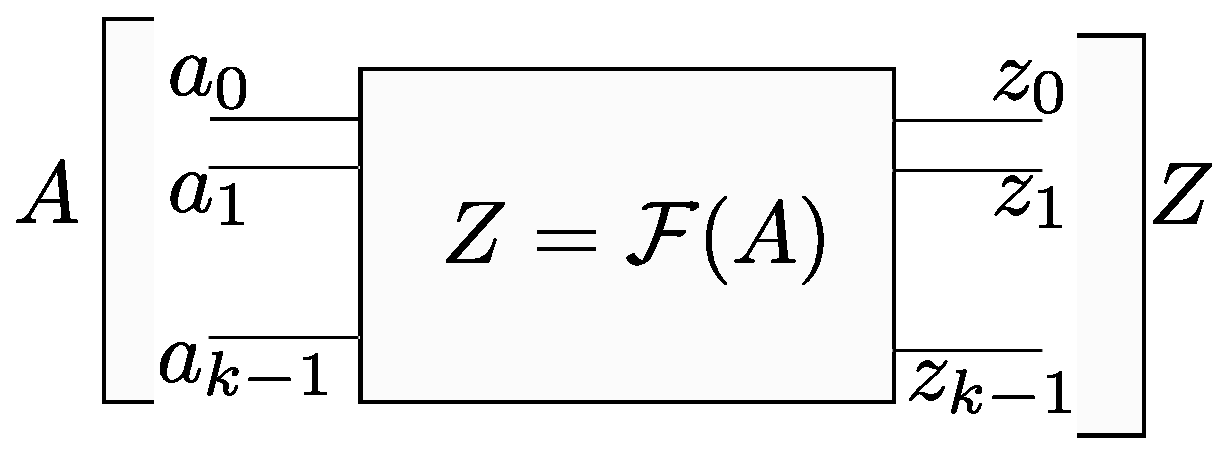
\includegraphics[width=0.5\textwidth]{./figures/interpolate}
}
\caption{Derive the abstraction $Z=\Func(A)$}
\label{fig:abstractA_Z2}
\end{figure}
}

By modelling the the arithmetic circuit as a polynomial system in
$\Fkk[x_1,x_2,\cdots,x_d]$, the abstraction problem 
can be solved using a \Grobner basis computation using an
abstraction term order. 
However, as computing a \Grobner basis is computationally
expensive, this approach is directly  applicable only to Galois field arithmetic
circuits no larger than $40$-bits.

\section{Problem Statement}

\begin{itemize}
\item  Given a gate-level combinational, acyclic circuit $C$ with $n$ word-level
$k$-bit inputs,
$A_1,\dots, A_n \in \Fkk$
and one $k$-bit output $Z$.
\item Pick a primitive, irreducible polynomial $P(x)$ over $\F_2[x]$ of degree $k$ 
to construct $\Fkk$ (these polynomials are known).
Let $P(\alpha) = 0$, where $\alpha \in \Fkk$ is a root of the irreducible
polynomial $P$.
\item The bit-level primary inputs of the circuit are denoted
$\{a_{0}^{i},a_{1}^{i},\dots,a_{k-1}^{i}\}$, for $1\leq i \leq n$;
the bit-level primary outputs are $\{z_0, \dots, z_{k-1}\} = Z$. 
Note that all $a_{j}^{i}, z_j \in \F_2$ for $0\leq j < k$.
\item Find the word-level polynomial function $\Func$ over $\Fkk$ 
computed by $C$ in the form of $Z=\Func(A_1, \dots, A_n)$.
\end{itemize}

In order for a combinational circuit $C$ to compute a function $f$ over the 
Galois field $\Fkk$, $C$ must have any number of 
$k$-bit word-level inputs and one $k$-bit word-level output.
Since every function over $\Fkk$ is a polynomial function, 
$C$ has a word-level polynomial representation over $\Fkk$.
The goal is to derive this word-level polynomial representation $\Func$ 
computed by a given combinational circuit over a 
given $\Fkk$.

%The proposed approach is generic enough to abstract the implementation of any
%combinational Galois field arithmetic circuit.
For the purpose of explaining the proposed abstraction approach, 
this chapter explores its application to Galois field multiplier circuits, 
which are described in Chapter \ref{ch:prelim}, 
as they form the core of most cryptographic computations in ECC and are 
notoriously hard to verify. In this case, $P(x)$ is chosen to be the same
primitive polynomial over which the circuit was designed.

\begin{Example}
Consider our problem statement as it applies to a multiplier 
circuit over $\Fkk$. The specification of the circuit is unknown.
\begin{itemize}

\item Given the Galois field $\Fkk$ and the corresponding
  irreducible polynomial $P(x)$. Let $P(\alpha) = 0$.

\item  Given a gate-level combinational circuit. The bit-level primary
  inputs of the circuit are $\{a_0, \dots, a_{k-1}, ~b_0, 
  \dots, b_{k-1}\}$, and the bit-level primary outputs are 
$\{z_0, \dots, z_{k-1}\}$; thus all $a_i, b_i, z_i \in \F_2$.

\item $A$ and $B$ denote the $k$-bit word-level inputs and $Z$ is the
$k$-bit word-level output. Therefore, 
$A = a_0 + a_1\alpha + \dots + a_{k-1}\alpha^{k-1}$,
$B = b_0 + b_1\alpha + \dots + b_{k-1}\alpha^{k-1}$, and 
$Z = z_0 + z_1\alpha + \dots + z_{k-1}\alpha^{k-1}$ with $A,B,Z \in \Fkk$.

\item Find the word-level polynomial function $\Func$ that this circuit 
implements over $\Fkk$.
The polynomial must be in the form of $Z=\Func(A,B)$. Since, in this case, 
the circuit is a multiplier, this resulting polynomial will be $Z=A\cdot B$.

\end{itemize}
\end{Example}

\section{Circuit Polynomial Modeling}

Given a gate-level implementation of a circuit,
we map each gate-level
Boolean operator in the circuit ($NOT$, $AND$, $OR$, $XOR$) to a polynomial 
over $\F_2$ using the following
one-to-one mapping over $\mathbb{B} \rightarrow \mathbb{F}_2$ : 
\begin{equation}
\label{b2poly}
\begin{split}
NOT :&~\neg a \rightarrow a+1 \pmod 2  \\   
AND :&~a \wedge b \rightarrow a\cdot b \pmod 2  \\ 
OR :&~a \vee b \rightarrow a+b+a\cdot b \pmod 2  \\
XOR :&~a \oplus b \rightarrow a+b \pmod 2 
\end{split}
\end{equation}
where $a,b \in \mathbb{F}_{2}=\{0,1\}$.
Note that the equation $c=\mathcal{F}(a,b)$ is written in polynomial
form as $c-\mathcal{F}(a,b)=c+\mathcal{F}(a,b)=0$, ~as $-1 \equiv +1
\pmod 2$.

\begin{Example}
Consider the equation with Boolean operators: 
\begin{equation}
z=a \oplus (b \vee c). \nonumber
\end{equation}

This equation modeled over $\F_2$ is:
\begin{equation}
z+a + b + c + b\cdot c=0 \nonumber
\end{equation}

Notice that the left-hand side expression is a polynomial in
$\F_{2}\left[a,b,c,z\right] \subset
\Fkk\left[a,b,c,z\right]$
\end{Example}

Secondly, we model the $k$-bit word-level inputs
and the $k$-bit word-level output of the given circuit as polynomial
expressions in $\mathbb{F}_{2^{k}}$ as shown in the problem statement.
If the $k$-bit word-level output of the circuit is denoted $Z$ which is 
composed of bit-level outputs 
$z_0, \dots , z_{k-1}$, the corresponding equation
is:
\begin{equation}
 Z = z_0 + z_1 \alpha + \dots + z_{k-1} \alpha^{k-1} \nonumber
\end{equation}
Once again, since $-Z = +Z \pmod 2$, this equation is modelled as:
\begin{equation}
Z + z_0 + z_1 \alpha + \dots + z_{k-1} \alpha^{k-1} = 0 \nonumber
\end{equation}

Likewise, for all word-level inputs $A_1,\dots,A_n$ we have
\begin{eqnarray}
A_1 + a_0^1 \alpha + \dots + a_{k-1}^1 = 0 \nonumber \\
\vdots \nonumber \\
A_n + a_0^n \alpha + \dots + a_{k-1}^n = 0 \nonumber 
\end{eqnarray}

Overall, a combinational circuit composed of $s$ Boolean gates
with $n$ $k$-bit inputs, $A_1, \dots , A_n$, and one $k$-bit output $Z$, 
is modeled as a polynomial system over $\mathbb{F}_{2^{k}}$ as follows:  

\begin{eqnarray}
 \left .  \begin{aligned}
f_1(x_1,x_2,\cdots, x_d)=0  \\
f_2(x_1,x_2,\cdots, x_d)=0  \\
\vdots  \\
f_s(x_1,x_2,\cdots, x_d)=0 \\
\end{aligned} 
\ \right\}
 &\qquad&  \text{\it Bit-level circuit constraints} \nonumber \\
 \left . \begin{aligned}
f_{Z}: Z+z_{0}+z_{1}\cdot \alpha,\cdots,{z_{k-1}}\cdot \alpha^{k-1}=0    \\
f_{A_1}:A_1+a_{0}^1+a_{1}^1\cdot \alpha+\cdots+a_{k-1}^1\cdot \alpha^{k-1}=0   \\
\vdots  \\
f_{A_n}:A_n+a_{0}^n+a_{1}^n\cdot \alpha+\cdots+a_{k-1}^n\cdot \alpha^{k-1}=0   \\
\end{aligned} 
\right\}
 &\qquad&  \text{\it Word-level designation} \nonumber \\
\end{eqnarray}


\begin{Example}
\label{exp:mul2bit}
Consider a 2-bit multiplier over ${\mathbb{F}}_{2^2}$ with
$P(x)=x^{2}+x+1$, given in Fig. \ref{fig:2bitmul}. Variables $a_0,
a_1, b_0, b_1$ are primary inputs, $z_0, z_1$ are primary outputs, and
$c_0, c_1, c_2, c_3, r_0$ are intermediate variables. 
%The gate $\otimes$
%corresponds to AND-gate, i.e. bit-level multiplication modulo 2. The
%gate $\oplus$ corresponds to XOR-gate, i.e. addition modulo 2.

\begin{figure}[H]
\centerline{
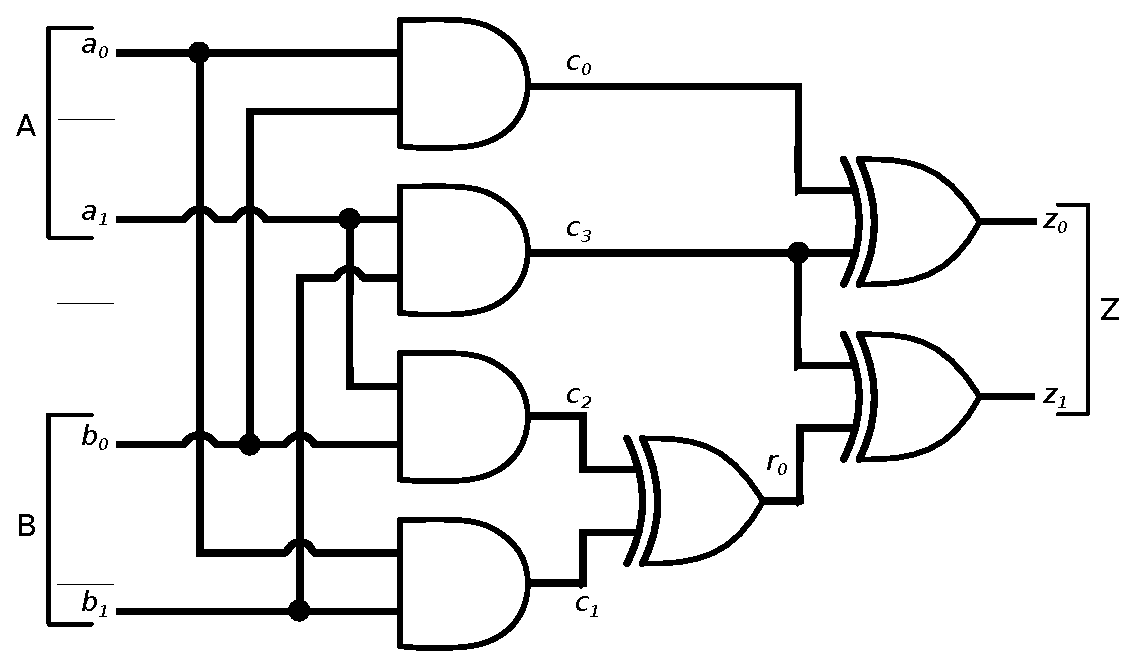
\includegraphics[scale=0.4]{./figures/2bitmasmult.eps}
}
\caption{ A 2-bit multiplier over ${\mathbb{F}}_(2^2)$.}
\label{fig:2bitmul}
\end{figure}

The circuit can be described using the following Boolean equations:
\begin{align*}
c_0=a_0 \wedge b_0,   \nonumber \\
c_1=a_0 \wedge b_1,   \nonumber \\
c_2=a_1 \wedge b_0, \nonumber \\
c_3=a_1 \wedge b_1,   \nonumber \\
r_0=c_1 \oplus c_2 ,      \nonumber \\
z_0=c_0 \oplus c_3,   \nonumber \\
z_1=r_0 \oplus c_3,    \nonumber
\end{align*}

With the mapping rules given in Equation \ref{b2poly}, 
the above equations are transformed into the following polynomials:
\begin{align*}
c_0+a_0 \cdot b_0,   \nonumber \\
c_1+a_0 \cdot b_1,   \nonumber \\
c_2+a_1 \cdot b_0,   \nonumber \\
c_3+a_1 \cdot b_1,   \nonumber \\
r_0+c_1 + c_2 ,      \nonumber \\
z_0+c_0 + c_3,   \nonumber \\
z_1+r_0 + c_3,   \nonumber
\end{align*}

Therefore, our overall polynomial system is:
\begin{eqnarray}
 \left .  \begin{aligned}
f_1: c_0+a_0 \cdot b_0  \\
f_2: c_1+a_0 \cdot b_1  \\
f_3: c_2+a_1 \cdot b_0  \\
f_4: c_3+a_1 \cdot b_1  \\
f_5: r_0+c_1 + c_2		\\
f_6: z_0+c_0 + c_3		\\
f_7: z_1+r_0 + c_3		   
 \end{aligned} 
\ \right\}
 &\qquad&  {\text {\it Bit-level circuit constraints}} \nonumber \\
 \left . \begin{aligned}
f_{A}: A+a_0+a_1\cdot \alpha  \\ 
f_{B}: B+b_0+b_1\cdot  \alpha  \\
f_{Z}: Z+z_0+z_1\cdot \alpha
 \end{aligned} 
\right\}
 &\qquad&  {\text {\it Word-Level designation}} \nonumber \\
\end{eqnarray}

\end{Example}

\section{Abstraction Formulation}

Let $S$ be the system of 
polynomials, 
$\{f_1,\dots,f_s,f_{A_1},\dots,f_{A_n},f_{Z}\}\subset \Fkk$, 
derived from the hardware
implementation of the Galois field arithmetic circuit over $\Fkk$.
This circuit performs some unknown function $f$ over 
$\Fkk$ in the form of $Z=\Func(A_1,\dots,A_n)$, where $Z$ is the $k$-bit 
output and $A_1,\dots,A_n$ are the $k$-bit inputs.
The polynomial representation of $\Func$ over $\Fkk$ is thus:

\begin{equation}
f_{\Func}: Z+\Func(A_1,\dots,A_n) \nonumber
\end{equation}

Since $f_{\Func}$ is ultimately derived from the circuit implementation, 
it agrees with the solution to the system of polynomials $\{S\}=0$, i.e.:
\begin{equation}
f_1=\dots=f_s=f_{A_1}=\dots=f_{A_n}=f_{Z}=0 \nonumber
\end{equation}
Thus, if we let $J=\langle f_1,\dots,f_s,f_{A_1},\dots,f_{A_n},f_{Z}\rangle$ 
be the ideal generated by $S$, 
$f_{\Func}$ {\bf vanishes} on the variety $V_{\Fkk}(J)$. 
Therefore, due to Proposition \ref{pro:iofv}, 
$f_{\Func}$ must be contained in the ideal of polynomials that vanish on
this variety, $f_{\Func} \in I(V_{\Fkk}(J))$. 

By applying Strong Nullstellensatz over $\Fkk$ (Theorem \ref{thm:sns}), 
$I(V_{\Fkk}(J))=J+J_0$ where
$J_0$ is the ideal generated by all vanishing polynomials in $\Fkk$. 
Recall that a vanishing polynomial in $\Fkk[x]$ is $x^q-x=x^q+x$. 
In our case, 
$\{x_1,\dots,x_d\} \in \F_2$ and $\{A_1,\dots,A_n,Z\} \in \Fkk$.
Thus, for $\Fkk[x_1,\dots,x_d,A_1,\dots,A_n,Z]$: 
\begin{equation}
J_0 = \langle x_1^2+x_1,\dots,x_d^2+x_d, A_1^{2^k}+A_1,\dots,A_n^{2^k}+A_n,Z^{2^k}+Z\rangle \nonumber
\end{equation}

The generators of the ideal sum $J+J_0$ are simply the combination of the 
generators of $J$ and the generators $J_0$.

\begin{Example}
\label{exp:finalMul2Bit}
Let us re-consider Example \ref{exp:mul2bit}. First, polynomials are
extracted from the circuit implementation as
shown in Example \ref{exp:mul2bit}. These polynomials represent the
ideal $J$. Along with the ideal of vanishing polynomials $J_0$, 
the following polynomials represent the generators 
of $J+J_0$ for the multiplier circuit. 

\begin{eqnarray}
 \left .  
	\begin{aligned}
		f_1:c_0+a_0 \cdot b_0  \\
		f_2:c_1+a_0 \cdot b_1  \\
		f_3:c_2+a_1 \cdot b_0  \\
		f_4:c_3+a_1 \cdot b_1  \\
		f_5:r_0+c_1 + c_2		\\
		f_6:z_0+c_0 + c_3		\\
		f_7:z_1+r_0 + c_3		
	\end{aligned} 
 \ \right\}
 &\qquad&  {\it  \text{Bit-level circuit constraints} ~(\subset J)} \nonumber \\
 \left . 
	\begin{aligned}
		f_{A}:A+a_0+a_1\cdot \alpha   \\ 
		f_{B}:B+b_0+b_1\cdot \alpha  \\ 
		f_{Z}:Z+z_0+z_1\cdot \alpha   
	\end{aligned} 
 \right\}
 &\qquad&  {\it  \text{Word-level designation} ~(\subset J)} \nonumber \\
  \left . 
	\begin{aligned}
		a_0^2-a_0, ~a_1^2-a_1,~b_0^2-b_0, ~b_1^2-b_1   \\ 
		c_0^2-c_0, ~c_1^2-c_1,~c_2^2-c_2, ~c_3^2-c_3  \\ 
		r_0^2-r_0, ~z_0^2-z_0,~z_1^2-z_1    \\ 
		A^4-A, ~B^4-B ,~Z^4-Z		  
	\end{aligned} 
 \right\}
 &\qquad&  {\it \text{vanishing polynomials} (J_0)} \nonumber
\end{eqnarray}
 
\end{Example}

The variety $V_{\Fq}(J)$ is
the set of all consistent assignments to the nets (signals) in the
circuit $C$. If we {\it project this variety on the word-level input and
output variables of the circuit $C$, we essentially generate the
function $\Func$ implemented by the circuit.} Projection of varieties from
$d$-dimensional space $\Fq^d$ onto a lower dimensional subspace
$\Fq^{d-l}$ is equivalent to {\it eliminating $l$ variables} from the
corresponding ideal. This can be done by computing a \Grobner basis
of the ideal with elimination ordering, as described in the 
Elimination Theorem (Theorem \ref{thm:elimth}).
Thus, we can find the polynomial 
$f_\Func:Z+\Func(A_1,\dots,A_n)$ by computing the \Grobner
basis of $J+J_0$ using the proper elimination ordering.

The proposed elimination order for 
abstraction is defined as the {\bf abstraction term order}. 

\begin{Definition}
\label{def:ato}
Given a circuit $C$,
let $x_1, \dots, x_d$ denote all the bit-level variables, 
let $A_1,\dots,A_n$ denote the $k$-bit word-level inputs, 
and let $Z$ denote the $k$-bit word-level output. 
Using the partial variable order 
$\{x_1, \dots, x_d\} > Z > \{A_1, \dots, A_n\}$,
where any refinement of the order will do,
impose a lex term order $>$ on the polynomial ring 
$R = \Fq[x_1, \dots, x_d, Z, A_1, \dots, A_n]$. 
This elimination term order $>$ is defined as
the {\bf Abstraction Term Order}. The relative ordering among $x_1,
\dots, x_d$ is not important and can be chosen arbitrarily. Likewise,
the relative ordering among $A_1, \dots, A_n$ is also unimportant.
\end{Definition}

\begin{Theorem}
{\bf Abstraction Theorem:} Using the setup and notations above,
compute a \Grobner basis $G$ of ideal $(J+J_0)$ using the abstraction term 
order $>$. Then: \\
(i) For every word-level input $A_i$, $G$ must contain the vanishing 
polynomial $A_i^q - A_i$ as the only polynomial with $A_i$ as its only 
variable;\\
(ii) $G$ must contain a polynomial of the form 
$Z + \mathcal{G}(A_1,\dots,A_n)$; and\\ 
(iii) $Z + \mathcal{G}(A_1,\dots,A_n)$ is such that 
$\Func(A_1,\dots,A_n) = {\mathcal{G}}(A_1,\dots,A_n),
\forall A_1,\dots,A_n \in \Fq$. 
In other words, ${\mathcal{G}}(A_1,\dots,A_n)$ and $\Func(A_1,\dots,A_n)$ are
equal as polynomial functions over $\Fq$.
\label{thm:abs}
\end{Theorem}

\begin{Proof}\
(i) For $A_i$, $A_i^q-A_i$ is a given generator of $J_0$. 
  $A_1,\dots,A_n$ are also 
  the last variables in the abstraction term order. Moreover, $A_i$ is an
  input to the circuit, so $A_i$ is an independent variable. As a result, 
  $G_{d+1} = G \cap\Fkk[A_1,\dots,A_n] = \{A_1^q - A_1,\dots,A_n^q-A_n\}$.

(ii) Since $f:Z + \Func(A_1,\dots,A_n)$ is a polynomial representation of
  the function of the circuit, $Z + \Func(A_1,\dots,A_n) \in J + J_0$, as
  described above. Therefore, according to the definition of a
  \Grobner basis, the leading term of $Z +
  \Func(A_1,\dots,A_n)$ (which is $Z$) should be divisible by the leading
  term of some polynomial $g_i \in G$. The only way $lt(g_i)$ can
  divide $Z$ is when $lt(g_i) = Z$ itself. Moreover, due to our
  abstraction (lex) term order, $Z > A > \dots > A_n$, so this polynomial 
  must be of the form $Z + {\mathcal{G}}(A_1,\dots,A_n)$. 

(iii) As $Z = \Func(A_1,\dots,A_n)$ represents the function of the circuit, 
  $Z + \Func(A_1,\dots,A_n) \in J + J_0$. 
  Moreover, $V(J + J_0) \subset V(Z + \Func(A_1,\dots,A_n))$. 
  By projecting this variety $V(J + J_0)$ onto the co-ordinates
  corresponding to $(A_1,\dots,A_n, Z)$, we obtain the {\it graph of the
  function} $(A_1,\dots,A_n) \mapsto \Func(A_1,\dots,A_n)$ 
  from $\Fkk \rightarrow \Fkk$. Since $Z + {\mathcal{G}}(A)$ is an element 
  of the \Grobner basis of $J + J_0$, 
  $V(J + J_0) \subset V(Z + {\mathcal{G}}(A_1,\dots,A_n))$. Therefore,
  $Z = {\mathcal{G}}(A_1,\dots,A_n)$ gives the same function as 
  $Z = \Func(A_1,\dots,A_n)$, for all $A_i \in \Fkk$.
\end{Proof}

As a consequence of the Abstraction Theorem, computing a \Grobner
basis $G$ of $J + J_0$ using the abstraction term order finds
a polynomial of the form $Z + \G(A_1,\dots,A_n)$ in the \Grobner basis, 
such that $Z = \G(A_1,\dots,A_n)$ is a polynomial representation of the 
circuit. However, if the \Grobner basis is not reduced, it is possible to 
obtain multiple polynomials in $G$ of the form 
$Z + \G _1(A_1,\dots,A_n), Z + \G _2(A_1,\dots,A_n), \dots,$;
all of which correspond to the same function. 

\begin{Corollary}
By computing a {\bf reduced} \Grobner basis $G_r$ of $J + J_0$, 
$G_r$ will contain one and only one polynomial in of the form 
$Z + \G(A_1,\dots,A_n)$, such that $Z = \G(A_1,\dots,A_n)$ is the 
{\bf unique, minimal, canonical} representation of the function 
$\Func$ implemented by the circuit.  
\end{Corollary}

\begin{Proof}
Any function $f: \Fkk^d \to \Fkk$ has a unique canonical 
representation as polynomial $P_f \in \Fkk[x_1, ..., x_d]$ such that all 
its nonzero monomials are of the form $x_1^{i_1}\cdots x_d^{i_d}$ where $0 
\leq i_j \leq q-1$, for all $j=1, \ldots d$.

%Let $q_i$ be a power of $2$ for $i=1, \ldots, d$. 
Let $J_0$ be the 
ideal of all polynomials that vanish over $\Fkk[x_1, \ldots, x_d]$.
The generators of $J_0$ are polynomials in the form $x_i^{2^q_i}-x_i$,
where $q_i$ is the datapath size of $x_i$.
Then these generators also form a reduced Gr\"obner basis for $J_0$.
This implies that the elements $A_h^{2^k}-A_h, 1 \leq h \leq n$ will 
have to be part of the reduced Gr\"obner basis of $J+J_0$.

Corollary 1.8.6 in~\cite{gb_book} shows that the obtained element $\Func
(A_1,..., A_n)$ that is reduced modulo
$A_h^{2^k}-A_h, 1 \leq h \leq n$. Thus, the polynomial representation of 
$\Func$ in the reduced \Grobner basis is the unique canonical 
representation.
\end{Proof}

\begin{Example}
Consider the $2$-bit multiplier Example 
\ref{exp:finalMul2Bit}, for which we have already generated $J+J_0$. 
We apply abstraction term order $>$, i.e a lex order with
"bit-level variables" $>$ "Output Z" $>$ "Inputs A, B".

When we compute the reduced \Grobner basis, $G_r$, of \{$J + J_0$\} with 
respect to this ordering, $G_r$ = \{$g_1, \dots, g_{14}\}:$
\begin{align*}
g_1: B^4+B; 
~~g_2: b_0+b_1 \alpha + B; 
~~g_3: a_0+a_1 \alpha + A;  \nonumber \\
~~g_4: c_0+c_1 \alpha + c_2 \alpha + c_3(\alpha+1)+Z;
g_5: r_0+c_1+c_2; 
~~g_6: z_0+c_0+c_3; \nonumber \\
~~g_7: z_1+r_0+c_3; 
~~{\bf g_8: Z+A\cdot B};
~~g_9: b_1+B^2+B; 
~~g_{10}: a_1+A^2+A; \nonumber \\
~~g_{11}: c_3+a_1\cdot b_1
g_{12}: c_2+a_1\cdot b_1 \alpha + a_1 \cdot B; 
~~g_{13}: c_1+a_1\cdot b_1 \alpha +b_1 A; 
~~g_{14}: A^4+A  \nonumber
\end{align*}

$g_8=Z+A\cdot B$ is the {\bf canonical, word-level polynomial } 
representing the function performed by the multiplier $Z=A\cdot B$.
\end{Example}

Consolidating our results, the proposed abstraction approach is described
as follows: 

\begin{enumerate}
\item Given a bit-level implementation of a Galois field arithmetic circuit 
$C$ over a given $\Fkk$, 
with $k$-bit output $Z$ and $k$-bit inputs $A_1,\dots,A_n$. 
\item $C$ performs some unknown function $Z=\Func(A_1,\dots,A_n)$.
\item Model the the circuit as a system of polynomials 
$\{f_1,\dots,f_s\}\subset \Fkk[x_1,\dots,x_d, Z, A_1, \dots, A_n]$ as 
described above and let $J$ be the ideal generated by these polynomials. 
\item Let $J_0$ be the ideal generated by all vanishing polynomials of 
$\Fkk$. 
\item By computing a reduced \Grobner basis $G_r$ of ideal $J+J_0$ using 
{\bf abstraction term order}, 
the word-level polynomial $Z+\Func(A_1,\dots,A_n)$ will be found in $G_r$.
\end{enumerate}

\section{Experimental Results: Validation of the Approach}

Our experiments take, as inputs, Mastrovito \cite{mastro:1989} multiplier 
circuits of various word sizes $k$. Each multiplier performs the polynomial 
function $Z = \Func(A,B) = A \cdot B$ over a Galois field, 
where $Z$ is the $k$-bit 
output and $A$ and $B$ are the $k$-bit inputs. We extract the 
Boolean gate-level operators $J$ and vanishing polynomials $J_0$.
Then we compute the reduced \Grobner basis $G_r$ of $J + J_0$
with respect to abstraction term order $>$. The resulting $G_r$ contains a 
polynomial $Z + A\cdot B$. 

The experiments were designed as scripts in the computer algebra tool, 
{\sc Singular} \cite{DGPS}, which provides functionality for polynomial
computations over rings and fields. This tool provides a number of efficient 
polynomial algorithms. The ring $\Fkk[x_1,\dots,x_f,\allowbreak Z,A,B]$ is defined over
the abstraction ordering, using the same primitive polynomial 
(``minpoly'' in Singular) $P(X)$ that was used to design the Galois field multiplier. 
Ideals  $J$ and $J_0$ were provided using their generating polynomials and the
the reduced \Grobner basis computation of $J+J_0$ was performed
using the ``slimgb'' command.

The experiments were conducted on a 64-bit Ubuntu machine running a 2.4GHz 
processor with 8GB of memory. We applied our approach to
abstract the canonical, polynomial representation of Mastrovito 
multipliers of various sizes.
Our machine was unable to perform the 
computations of the Gr\"obner basis of multipliers beyond $40$-bit word 
inputs. 

\begin{table}[H]
\label{tab:slimgb}
	\begin{center}
	    \caption{Run-time of Gr\"obner Basis Computation of Mastrovito Multipliers in Singular using Abstraction Term Order $>$.}\label{tab:sT}
	    \begin{tabular}{|c|c||c|} 
	        \hline
		Word Size ($k$) & Number of Polynomials ($d$) & Computation Time (minutes)   \\
		\hline
	        $16$	&  $1,871$  & $2.4$ \\
		$24$	&  $3,135$  & $12$  \\
	        $32$	&  $5,549$  & $22.6$ \\
	        $40$	&  $8,587$  & $266$ \\
		$48$	& $12,327$  & NA (Out of Memory) \\
	        \hline
	    \end{tabular}
	\end{center} 
\end{table}

\section{Conclusions}
The above approach is guaranteed to find a canonical, word-level 
representation of the function $\Func$ performed by a circuit $C$ over 
$\Fkk$. However, the \Grobner basis computation is prohibitively complex for
circuits of practical sizes. The next chapter proposes a 
method to overcome the complexity of the \Grobner
basis computation in order to make this abstraction approach scalable.

\chapter{Overcoming Grobner Basis Complexity for Abstraction} \label{ch:improv}

Computing a \Grobner basis is prohibitively expensive for large circuits. 
%The worst-case complexity of computing $GB(J + J_0)$
%in $\Fq[x_1, \dots, x_d]$ is known to be bounded by $q^{O(d)}$
%\cite{gao:gf-gb-ms}, which is prohibitive over large
%fields. 
The approach from the last 
chapter is limited only to small circuits, with data-paths no larger than 
$40$-bits. 
A full \Grobner basis computation results in numerous polynomials, but
the abstraction approach ``searches'' for only one
polynomial ($Z + \G(A)$) in the basis. This motivates an investigation into
whether it is possible to {\it  guide a sequence of $Spoly(f,
  g)\xrightarrow{J+J_0}_+ r$  computations} to arrive at the desired
word-level polynomial. This chapter describes this 
{\it smaller subset} of computations, which are derived from a \Grobner basis 
analysis, to find the word-level polynomial of the function performed by a 
given circuit. The improved approach can abstract canonical word-level 
representations of circuits up to $571$ bits, 
corresponding to the largest NIST-specified ECC standard. 

\section{Improving the Abstraction Approach}
Consider the word-level abstraction problem formulation from 
Chapter \ref{ch:abstract}. $J$ is the ideal 
generated by all polynomials derived from the circuit implementation and 
$J_0$ is the ideal of all the vanishing polynomials of 
every variable in the ring. 
The computation of the reduced \Grobner basis of $J+J_0$ over $\Fq$ 
has the following known complexity\cite{gao:gf-gb-ms}:

\begin{Theorem}
Let $J+J_0 = \langle f_1, \dots, f_s, ~x_1^q - x_1, \dots, x_d^q -
x_d\rangle \subset \Fq [x_1, \dots, x_d]$ be an ideal. The time and
space complexity of Buchberger's algorithm to compute a \Grobner
basis of $J+J_0$ is bounded by $q^{O(d)}$.
\end{Theorem}

In our case $q = 2^k$, and when $k$ and $d$ are large, this complexity 
makes abstraction infeasible.

Recall that Buchberger's algorithm \cite{buchberger_thesis} for 
computing \Grobner bases depends on the computation of an $S$-polynomial, 
which is then reduced by all the polynomials in the basis. 

\begin{equation}
Spoly(f_{i}, f_{j}) \stackrel{G'}{\textstyle\longrightarrow}_+r \nonumber
\end{equation}
where
\begin{eqnarray}
Spoly(f,g)=\frac{L}{lt(f)}\cdot f - \frac{L}{lt(g)}\cdot g \nonumber \\ 
\nonumber \\
L=lcm(lt(f),lt(g)) \nonumber
\end{eqnarray}

A new polynomial is added to the basis when the remainder of the $Spoly$
reduction, $r$, is non-zero.

Notice that our approach searches
for only one polynomial $f_\Func:Z+\Func(A_1,\dots,A_n)$, and it does
by computing the entire reduced \Grobner basis, $G=\{g_1,\dots,g_m\}$ and
finding $f_\Func\in \{g_1,\dots,g_m\}$.
This motivates us to
investigate whether it's possible to {\it  guide a sequence of 
$Spoly(f,g)\xrightarrow{J+J_0}_+ r$  computations} to arrive at the desired
word-level polynomial, without considering other polynomials in the
generating set. 

Numerous improvements have been introduced to improve the efficiency of 
Buchberger's algorithm. One of these is the product criterion, the results
of which we exploit for our approach.

\begin{Lemma}
\label{lemma:prodcriteria}
[Product Criterion \cite{productc:1979}] Let $\mathbb{F}$ be any
field, and $f, g \in \mathbb{F}[x_1,\cdots,x_d]$ be polynomials. If
the equality $lm(f) \cdot lm(g) = LCM(lm(f), lm(g))$ holds, then
$Spoly(f,g)\stackrel{G}{\textstyle\longrightarrow}_+ 0.$ 
\end{Lemma}

The above result states that when the leading monomials of $f, g$ are
relatively prime then 
$Spoly(f, g)$ always reduces to 0 modulo $G$. In this case,
$Spoly(f, g)$ need not be considered in Buchberger's algorithm, and thus
the computation is avoided. 
Recall that in the Abstraction Term Order (Definition \ref{def:ato}),
we have ``circuit variables $x_1, \dots, x_d$'' $>$ ``word-level output''
$>$ ``word-level inputs'', where the
relative ordering among  $x_1, \dots, x_d$ is not important. This ordering
is now further refined to exploit the product criteria.

Given an acyclic combinational circuit, an ordering can be applied to the 
bit-level variables, $\{x_1,\dots,x_d\} \in \F_2$, 
based on their topological position in the circuit. In a {\it reverse topological
ordering}, the output variable of the gate will always come earlier in the
ordering than any of its input variables.
%This is denoted {\bf topological ordering}.

%\begin{Definition}
%Given a Boolean combinational circuit, let the topological location of the 
%bit-level variable $x$, denoted as $TL(x)$, be the 
%maximum number of Boolean logic gates that any path from any input must 
%pass to reach the variable. Then the variable ordering 
%\begin{equation}
%x>y : TL(x)<TL(y) 
%\end{equation}
%is denoted {\bf topological ordering}. Likewise, the ordering 
%\begin{equation}
%x>y : TL(x)>TL(y) 
%\end{equation}
%is a {\bf reverse topological ordering}.
%\label{def:topord}
%\end{Definition}
%\begin{Example}
%Consider the combinational circuit shown in Figure \ref{fig:topo}.
%This circuit has two bit-level inputs
%$a$ and $b$, intermediate variable $c$; and output $z$.

%\begin{figure}[H]
%\centerline{
%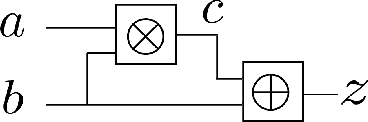
\includegraphics[scale=0.6]{./figures/topoExample.png}
%}
%\caption{Boolean combinational circuit.}
%\label{fig:topo}
%\end{figure}

%Then:
%\begin{eqnarray}
%TL(a)=0 \nonumber \\
%TL(b)=0 \nonumber \\
%TL(c)=1 \nonumber \\
%TL(z)=2 \nonumber
%\end{eqnarray}

%Thus, $a > b > c > z$ is a topological ordering. 
%Since $TL(a)=TL(b)$, $b > a > c > z$ is also a topological 
%ordering. 

%Likewise, $z > c > a > b$ and $z > c > b > a$ are considered reverse
%topological orderings.
%\end{Example}


\begin{Definition}
\label{def:rato}
{\bf Refined Abstraction Term Order (RATO) $>_r$:} 
%Starting from the primary
%outputs of the circuit $C$, perform a reverse topological traversal
%toward the primary inputs. Order each variable of the circuit
%according to its reverse topological level: i.e. $x_i > x_j$ if $x_i$
%appears earlier in the reverse topological order.
Given a circuit $C$, apply a reverse topological ordering to the bit-level
variables $\{x_1, \dots, x_d\}$.
Then, impose a lex term
order $>_r$ on $\Fq[x_1, \dots, x_d, Z, A_1, \dots, A_n]$ with ``circuit 
variables ordered reverse topologically'' $>$ 
``output word-level variable'' $>$ ``input word-level variables''. 
%This term order $>_r$ is called the {\bf refined abstraction term order (RATO)}.
\end{Definition}

Let $F$ be the set of polynomials which generate $J$, i.e. $J=<F>$. 
When RATO is applied, 
we find that all 
{\it bit-level circuit constraint
polynomials} in $F$ have leading terms that are relatively prime to each 
other. Since we are using a
reverse topological variable ordering with lex term ordering, these 
polynomials are in the 
form of $f_i = x_i + \text{tail}(f_i)$, where $x_i$ is the output of a gate $f_i$, 
and thus the following
proposition from {\it Lv's} work \cite{lv:phd} can be applied.

\begin{Proposition} \label{prop:top-order}
Let $C$ be any arbitrary combinational circuit. Let $\{x_1, \dots,
x_d\}$ denote the set of all variables (signals) in the circuit,
i.e. the primary input, intermediate and primary output
variables. Perform a {\bf reverse topological traversal} of the
circuit and order the variables such that $x_i > x_j$ if $x_i$ appears
earlier in the reverse topological order. Impose a lex term order to
represent the Boolean expression for each gate as a polynomial $f_i$;
then $f_i = x_i + \text{tail}(f_i)$. Then the set of all polynomials
$\{f_1, \dots, f_s\}$ forms a Gr\"obner basis, as $lt(f_i)$ and $
lt(f_j)$ for $i\neq j$ are relatively prime. 
\end{Proposition}

\begin{Example}
Consider the $2$-bit multiplier from Example 
\ref{exp:finalMul2Bit}. With RATO applied, the bit-level circuit constraint
polynomials in $F$, where $J=<F>$, are:
\begin{eqnarray}
		f_1:c_0+a_0 \cdot b_0 \nonumber \\
		f_2:c_1+a_0 \cdot b_1 \nonumber \\
		f_3:c_2+a_1 \cdot b_0 \nonumber \\
		f_4:c_3+a_1 \cdot b_1 \nonumber \\
		f_5:r_0+c_1 + c_2		\nonumber \\
		f_6:z_0+c_0 + c_3	\nonumber	\\
		f_7:z_1+r_0 + c_3	\nonumber	
\end{eqnarray}
The leading terms of $f_1,\dots,f_7$ are relatively prime to each other.
\label{exp:2bitmulrato}
\end{Example}

Let $F_0$ be the set of polynomials which generate $J_0$, i.e. $J_0=<F_0>$.
In $F\cup F_0$, for every polynomial $f_i = x_i + \text{tail}(f_i)$ 
in $F$ there is a vanishing polynomial $v_i = x_i^2+x_i$ in $F_0$; 
$f_i$ and $v_i$ have leading terms which are not relatively prime.
In this case, 
\cite{lv:phd} shows that $Spoly(x_i+\text{tail}(f_i), x_i^{2^k}-x_i)
\stackrel{J,J_0}{\longrightarrow}_+ r$ always produces $r=0$, and thus can
be excluded from the \Grobner basis computation.

\begin{Theorem}
\label{thm:lvcontrib}
Let $q = 2^k$, and let $\Fq[x_1, \ldots, x_d]$ be a ring on
which we have a reverse topological lex order. Let $I$ be a subset of $\{1,
\ldots, d\}$. For all $i \in I$, let $f_i = x_i +P_i$ (where $P_i =
\text{tail}(f_i)$) such that  all indeterminates $x_j$  that appear in
$P_i$ satisfy $x_i > x_j$.  Then the set $G = \{f_i :  i  \in I\} \cup
\{x_1^q-x_1, \ldots, x_d^q-x_d\}$ is a Gr\"obner basis. 
\end{Theorem}

The proof is given in \cite{lv:phd} and is reproduced here:

\begin{Proof}
Given a system of polynomials derived from a circuit over 
$\Fq[x_1, \ldots, x_d]$, where $\{x_1,\dots,x_d\}$ are bit-level variables.
Apply a reverse topological lex ordering to $\{x_1,\dots,x_d\}$. 
Let $x_i$ be the output of a Boolean logic gate for some $1\leq i \leq d$.
Let $f = x_i + P_i$ be the polynomial derived from this logic gate and
$g = x_i^q-x_i$ be vanishing polynomial of $x_i$.
Then $Spoly(f,g)=
x_i^{q-1} f - g = x_i^{q-1}P_i + x_i$. In what follows, it is important
to note that the indeterminates appearing in $P_i$ are all less than
$x_i$ over the given ordering.  

First,  $x_i^{q-1}P_i +x_i - x_i^{q-2}P_i(x_i+P_i)=x_i^{q-2}P_i^2 +x_i,$ 
which shows that 
$x_i^{q-1}P_i +x_i \stackrel{x_i+P_i}{\longrightarrow}  x_i^{q-2}P_i^2
+x_i.$  

Next, $x_i^{q-2}P_i^2 + x_i - x_i^{q-3}P_i^2(x_i+P_i)=
x_i^{q-3}P_i^3+ x_i.$ Continuing in this fashion, we get $x_iP_i^{q-1}
+x_i-P_i^{q-1}(x_i+P_i) = x_i + P_i^q,$ and finally 
$x_i+P_i^q -(x_i+P_i) = P_i^q-P_i.$ Hence, 
$$x_i^{q-1}P_i +x_i \stackrel{x_i+P_i}{\longrightarrow} x_i^{q-2}P_i^2
+x_i \stackrel{x_i+P_i}{\longrightarrow} x_i^{q-3}
+x_i \stackrel{x_i+P_i}{\longrightarrow} \cdots$$
$$\cdots \stackrel{x_i+P_i}{\longrightarrow}
P_i^q+x_i\stackrel{x_i+P_i}{\longrightarrow} P_i^q-P_i.$$ 


Over the finite field $\mathbb{F}_{q}$, $P_i^q-P_i$ is a vanishing
polynomial. Therefore, $P_i^q-P_i \in I(V(J_0))= \langle
x_1^q-x_1, \ldots, x_d^q-x_d\rangle$. Due to the product criterion
(Lemma \ref{lemma:prodcriteria}), $G_0=\{x_1^q-x_1, \ldots, x_d^q-x_d\}$ is
Gr\"obner basis. Therefore 
$P_i^q-P_i \stackrel{G_0}\rightarrow_+ 0$. 
\end{Proof}

Due to RATO, there exists a polynomial $f_{z_i}\in F$ which is the 
polynomial derived from a Boolean logic gate, where $z_i$ is the first 
variable in the ordering for some $0\leq i <k$. That is, $f_{z_i}: z_i+\text{tail}(f_{z_i})$.
\begin{Proposition}
Over RATO, the polynomial pair $(f_Z, f_{z_i})$ is the only critical pair
at the start of the \Grobner basis computation of $J+J_0$, where 
$f_{z_i}$ is the polynomial derived from the gate
\end{Proposition}
\begin{Proof}
Due to Theorem \ref{thm:lvcontrib} and the product criterion, 
a critical pair must come from a word level designation polynomial, 
$\{f_Z,f_{A_1},\dots,f_{A_n}\}$, and a polynomial derived from a Boolean logic
gate. The leading terms of the polynomials $\{f_{A_1},\dots,f_{A_n}\}$ are 
bit-level inputs to the circuit and thus are not the outputs of any gate.
Thus, the only critical pair if $f_Z$ and $f_{z_i}$, where $z_i$ is the first
variable in the ordering and is thus the leading monomial of $f_Z$.
\end{Proof}
%Thus, we are left with only a few options for an $Spoly$ at the  
%beginning of a \Grobner basis computation of $J+J_0$ with abstraction order
%$>$. Consider the {\it word-level designation polynomials} 
%$\{f_{Z},f_{A_1},\dots,f_{A_n}\}$ in $J$. Since all word-level variables 
%are found last in abstraction order, the leading monomial of each of these
%polynomials is some bit-level $x_d$. Thus there is a vanishing polynomial
%$x_d^2+x_d$ with the same leading monomial. Take $f_Z$ for example:

%\begin{eqnarray}
%f_{Z}: z_{0}+z_{1}\cdot \alpha,\cdots,{z_{k-1}}\cdot \alpha^{k-1}+Z \nonumber \\
%f_{v}: z_0^2+z
%\end{eqnarray}


%Thus, there are no valid $S$-polynomials which can be generated using
%the set $\{$bit-level constraints $\in J$,  $J_0\}$.
%So a valid $S$-polynomials must be generated using at least 
%one {\it word-level designation polynomial}, $f_Z,f_{A_1},\dots,f_{A_n}$.
%Consider the output word-level designation polynomial $f_Z$:
%\begin{equation}
%f_Z: Z+z_0+z_1\alpha+\dots+z_{k-1}\alpha^{k-1}
%\end{equation}
%Since all word-level variables 
%are found last in RATO, the leading monomial of $f_Z$ 
%has to be a bit-level output variable, $z_i$, for some $0\leq i < k$. 
%Since $z_i$ is the output of a Boolean logic gate, there 
%exists a polynomial $f_{z_i} \in J$ with $z_i$ as the leading monomial, 
%$f_{z_i}:z_i + \text{tail}(f_{z_i})$. $Spoly(f_Z,f_{z_i})$ is 
%a valid $S$-polynomial, and it has
%some interesting properties.

Thus, the first computation of the \Grobner basis is guaranteed to be 
$Spoly(f_Z,f_{z_i})\xrightarrow{F,F_0}_+ r$.
This computation has the following interesting property.

\begin{Proposition} \label{prop:reduce}
Normalize $f_Z$, i.e. $f_Z$=$f_Z/LC(f_Z)$. Then
\begin{eqnarray}
Spoly(f_Z,f_{z_i})\xrightarrow{F,F_0}_+ r & \text{is equivalent to} &
f_Z\xrightarrow{F-\{f_Z\},F_0} + r
\end{eqnarray}
\end{Proposition}

%% \begin{Proposition} \label{prop:reduce}
%% Let $C$ be any arbitrary combinational circuit with $k$-bit inputs 
%% $A_1,\dots,A_n$ and $k$-bit output $Z$. Model the circuit as a system of 
%% polynomials as described earlier.
%% Let $f_Z$ be the word-level 
%% designation polynomial $Z+z_0+z_1\alpha+\dots+z_{k-1}\alpha^{k-1}$. By
%% applying RATO, the leading monomial of $f_Z$ will be $z_i$ for some
%% $0\leq i < k$.
%% There exists a polynomial $f_{z_i}$ in the form of $z_i+\text{tail}$, 
%% which is the polynomial representation of the 
%% Boolean gate with output $z_i$.
%% %Then if $f_Z$ and $f_i$ is first minimized, i.e. $f_Z$=$f_Z/LC(f_Z)$, 
%% Then 
%% \begin{equation}
%% Spoly(f_Z,f_{z_i})\stackrel{J,J_0}{\longrightarrow}_+ r
%% \end{equation}
%% is equivalent to
%% \begin{equation}
%% %f_Z\stackrel{J-\{f_Z\},J_0}{\longrightarrow}_+ r
%% f_Z\xrightarrow{J-\{f_Z\},J_0} + r
%% \end{equation}
%% \end{Proposition}

\begin{Proof}
Assuming both $f_{z_i}$ and $f_Z$ are minimized, i.e. 
$LC(f_{z_i})=LC(f_Z)=1$, 
they are both in the form $z_i+P$ for some polynomial $P$.
Let $f=z_i+P_f$ and $g=z_i+P_g$ represent $f_{z_i}$ and $f_Z$ respectively.

(i) For $Spoly(f,g)$
\begin{equation}
L=LCM(LT(f),LT(g))=LM(f)=LM(g)=z_i
\end{equation}
so
\begin{eqnarray}
Spoly(f,g)&=&\frac{L}{lt(f)}\cdot f - \frac{L}{lt(g)}\cdot g \nonumber \\
&=&\frac{z_i}{z_i}\cdot f - \frac{z_i}{z_i}\cdot g \nonumber \\
&=&f + g \nonumber
\end{eqnarray}
Thus 
$Spoly(f_Z,f_{z_i})\stackrel{F,F_0}{\longrightarrow}_+ r$
is equivalent to 
$f+g\stackrel{F,F_0}{\longrightarrow}_+ r$.

(ii) For $f_Z\xrightarrow{F-\{f_Z\},F_0} + r$, since the leading term 
of $f_Z$ is $z_i$, the only polynomial in the set $\{F-\{f_Z\},F_0\}$
which can perform the first division is $f_{z_i}$. 
Again, denote $f_Z$ as $f$ and $f_{z_i}$ 
as $g$. According to the reduction algorithm, the remainder $r$ of 
$f\stackrel{g}{\longrightarrow}_+ r$ is:
\begin{eqnarray}
r &=& f-lt(f)/lt(g) \cdot g \nonumber \\
  &=& f-z_i/z_i \cdot g \nonumber \\
  &=& f-g \nonumber \\
  &=& f+g
\end{eqnarray}
Thus 
$f_Z\xrightarrow{F-\{f_Z\},F_0} + r$
is equivalent to 
$(f+g)\xrightarrow{F-\{f_Z\},F_0} + r$

(iii) Consider $(f+g)\xrightarrow{F,F_0} + r$. $f=z_i+P_f$ and 
$g=z_i+P_g$. So $f+g=2z_i+P_g+P_f=P_g+P_f$ no longer contains $z_i$ as the 
leading monomial. As a consequence of RATO, as 
reduction proceeds the remainder will never again contain 
$z_i$ since $z_i$ is the first variable in the ordering. 
Since the leading monomial of $f_Z$ is $z_i$, $f_Z$ will never be 
used for reduction. Therefore 
$(f+g)\xrightarrow{F,F_0}+ r$
is equivalent to 
$(f+g)\xrightarrow{F-\{f_Z\},F_0}+ r$

Thus, 
$Spoly(f_Z,f_{z_i})\stackrel{F,F_0}{\longrightarrow}_+ r$
is equivalent to
$f_Z\xrightarrow{F-\{f_Z\},F_0}_+ r$
\end{Proof}

%Due to the reverse-topological abstraction order, 
%since there is a $x_i + \text{tail}$ for every $x_i \in \{x_1,\dots,x_d\}$ 
%except the bit level inputs $a_0,\dots,a_k$,
%$f_Z\xrightarrow{J-\{f_Z\},J_0}+ r$ can only contain the bit-level
%inputs $a_0,\dots,a_k$, the word level inputs $A_1,\dots,A_n$, and the 
%word-level output $Z$. 
Thus, $f_Z\xrightarrow{F-\{f_Z\},F_0}_+ r$ is the first computational step 
of the abstraction.
The polynomial remainder $r$
will {\it not} contain any bit-level variable corresponding to the
output of any gate in the design;  i.e. primary output bits and
intermediate variables of the circuit do not appear in $r$. To prove
this, assume that a non-primary-input variable $x_j$ appears in a
monomial term $m_j$ in $r$. Since there always exists a polynomial
$f_j$ such that $f_j = x_j + \text{tail}(f_j)$, $lt(f_j)$
divides monomial $m_j$ and $m_j$ can be canceled. Therefore, all
such terms $m_j$ with non-primary-input bit-level variables can be
eliminated.  

Two cases need to be considered: 
\begin{enumerate}
\item Remainder $r$ only contains word-level variables:
  word-level output $Z$ and the word-level 
  inputs $A_1,\dots,A_n$. 
  Since RATO is lex with $Z > \{A_1,\dots,A_n\}$, the remainder $r$
  is the desired canonical polynomial representation,
  $Z + \Func(A_1,\dots,A_n)$.
\item Remainder $r$ contains both the bit-level primary
  input variables, as well as the word-level
  variables.  
\end{enumerate}

%We've found that for bug-free Galois field
%arithmetic circuits,
%when we compute $Spoly(f_{Z},f_{z_i})\stackrel{J,J_0}{\longrightarrow}_+ r$, 
%$r$ only contains variables in $A_1,\dots,A_n,Z$ and is thus {\bf canonical, 
%word-level polynomial } in the form of 
%$Z+\Func(A_1,\dots,A_n)$.

\begin{Example}
\label{exp:absGood}
Again consider the $2$-bit multiplier from Example 
\ref{exp:2bitmulrato}.
RATO for this example is
\begin{equation}
z_1 > z_0 > r_0 > c_0 > c_1 > c_2 > c_3 > a_0 > a_1 > b_0 > b_1 > Z > A > B 
\end{equation}
$F+F_0$ with RATO applied is:
\begin{eqnarray}
 \left .  
	\begin{aligned}
		f_1:c_0+a_0 \cdot b_0  \\
		f_2:c_1+a_0 \cdot b_1  \\
		f_3:c_2+a_1 \cdot b_0  \\
		f_4:c_3+a_1 \cdot b_1  \\
		f_5:r_0+c_1 + c_2		\\
		f_6:z_0+c_0 + c_3		\\
		f_7:z_1+r_0 + c_3		
	\end{aligned} 
 \ \right\}
 &\qquad&  {\it  \text{Bit-level circuit constraints} ~(\subset J)} \nonumber \\
 \left . 
	\begin{aligned}
		f_{A}:a_0+a_1\cdot \alpha + A  \\ 
		f_{B}:b_0+b_1\cdot \alpha + B \\ 
		f_{Z}:z_1\cdot \alpha + z_0 + Z  
	\end{aligned} 
 \right\}
 &\qquad&  {\it  \text{Word-level designation} ~(\subset J)} \nonumber \\
  \left . 
	\begin{aligned}
		a_0^2-a_0, ~a_1^2-a_1,~b_0^2-b_0, ~b_1^2-b_1   \\ 
		c_0^2-c_0, ~c_1^2-c_1,~c_2^2-c_2, ~c_3^2-c_3  \\ 
		r_0^2-r_0, ~z_0^2-z_0,~z_1^2-z_1    \\ 
		A^4-A, ~B^4-B ,~Z^4-Z		  
	\end{aligned} 
 \right\}
 &\qquad&  {\it \text{vanishing polynomials} (J_0)} \nonumber
\end{eqnarray}
Notice that the leading monomial of $f_Z$ is $z_1$, which is also the leading monomial 
of $f_7$.
Minimize $f_Z$, 
$f_{Zmin}=f_Z/\alpha = z_1 +z_0\cdot(\alpha+1)+Z\cdot(\alpha+1)$.
By computing the $S$-polynomial of $f_{Zmin}$ and $f_7$:
\begin{equation}
Spoly(f_{Zmin},f_{7})\stackrel{F,F_0}{\longrightarrow}_+ r \nonumber
\end{equation}
the remainder $r$ is $Z+A\cdot B$.

Likewise, if we reduce $f_{Z}$ by $F-\{f_Z\},F_0$, that is reduce it by all
generators in $J+J_0$ except $f_Z$:
\begin{equation}
f_{Z}\xrightarrow{F-\{f_Z\},F_0} + r \nonumber
\end{equation}
the remainder $r$ is $Z+A\cdot B$. 
\end{Example}

%As this abstraction process can be computed as a reduction procedure, we
%created a highly efficient reduction tool over $Fkk$. Using this tool, we
%are able to abstract word-level polynomial representations for bug-free 
%circuits up
%to $407$-bits in size. When applied to buggy circuits, however, 
%approach yields a polynomial which includes bit-level input variables.

\begin{Example}\label{ex:improve1}
Now consider a $2$-bit multiplier which has a {\bf bug}.
The output lines, $z_0$ and $z_1$, have been swapped, as shown in 
Figure \ref{fig:2bitmulbug} below:

\begin{figure}[H]
\centerline{
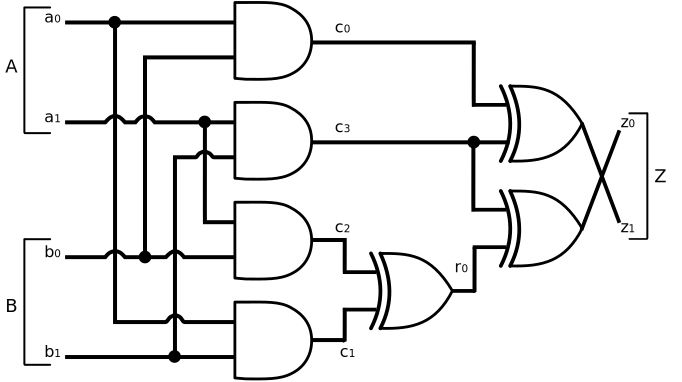
\includegraphics[scale=0.4]{./figures/2bitmasmultBUGswap}
}
\caption{ A buggy 2-bit multiplier over ${\mathbb{F}}(2^2)$.}
\label{fig:2bitmulbug}
\end{figure}

The polynomials in $F+F_0$ are the same as in Example \ref{exp:absGood} 
except for the following changes:
\begin{eqnarray}
f_6:z_1+c_0 + c_3	\nonumber	\\
f_7:z_0+r_0 + c_3	\nonumber	\\
f_Z:z_1 + z_0\cdot \alpha + Z  \nonumber	
\end{eqnarray}

$f_Z$ has common leading terms with $f_6$. Computing 
\begin{equation}
Spoly(f_Z,f_{6})\stackrel{F,F_0}{\longrightarrow}_+ r \nonumber
\end{equation}
gives remainder $r: a_1\cdot b_1 \alpha + a_1\cdot B \alpha + b_1 \cdot A \alpha + Z + A\cdot B$, which is the same result as computing
$f_Z\xrightarrow{F-\{f_Z\},F_0}_+ r$
\label{exp:2bitbugmulex}
\end{Example}

%%%%%%%%%%%%%%%%%%%%%%F4-STYLE REDUCTION%%%%%%%%%%%%%%%%%%%%%%%%%%%%%

\section{Improving Polynomial Division using $F4$-style Reduction}

The most intensive computational step in our proposed improvement 
is that of polynomial division $f_Z \xrightarrow{F-\{f_Z\},F_0}_+ r$. 
When the circuit $C$ is very large, the polynomial set
$\{F-\{f_Z\},F_0\}$ also becomes extremely large. This division
procedure then becomes the bottleneck in our abstraction approach.  
In principle, this reduction can be performed using contemporary
computer-algebra systems --- {\it e.g.},  the {\sc Singular}
\cite{DGPS} tool, which is widely used within the verification
community \cite{wienand:cav08} \cite{wedler:date11}
\cite{lv:date2012}. In our work, we have also performed experiments 
with {\sc Singular}. However, as in any ``general-purpose''
computer algebra tool, the data-structures are not specifically
optimized for circuit verification problems. Moreover, {\sc
  Singular} also limits the number of variables ($d$) that it can
accommodate in the system to $d < 32767$; this limits its
application to large circuits. Recent symbolic computation techniques \cite{lv:phd}
have shown improvements from employing the concept of $F4$-style 
polynomial reduction \cite{f4}.
Therefore, to further improve our
approach, we exploit this relatively recent concept, 
which implements polynomial division
using row-reductions on a matrix, to develop a custom
verification tool to perform this reduction
efficiently.

$Faug\grave{e}re$'s $F4$ approach \cite{f4} presents a new algorithm to
compute a Gr\"obner basis. It uses the same mathematical principles as
Buchberger's algorithm. However, instead of computing and reducing one 
$S$-polynomial at a time, it computes many $S$-polynomials in one
step and reduces them simultaneously using sparse linear algebra on a
matrix (triangulation). We can use this efficient reduction technique
to perform our reduction, $f_Z \xrightarrow{F-\{f_Z\},F_0}_+ r$, by 
representing and solving it on a matrix.
First, let us consider the following example that demonstrates the
main concepts behind the reduction approach of $F4$. 

\begin{Example}
{\it
Consider the {\it lex} term order with $x>y>z$ on the ring
${\mathbb{Q}}[x, y, z]$.  Given $F = \{f_1 = 2x^2 + y, f_2 = 3xy^2
-xy, f_3 = 4y^3 -1\}$, consider one step of Buchberger's algorithm:
$S(f_1, f_2) \xrightarrow{f_1, f_2, f_3}_+r$. We have, $Spoly(f_1,
f_2) = \frac{1}{3}x^2y + \frac{1}{2}y^3 = f_4$. The reduction
$Spoly(f_1, f_2)\stackrel{f_1, f_2, f_3}{\longrightarrow}_+
(-\frac{1}{6}y^2 + \frac{1}{8})$ is done as follows: 
Since $lt(f_1) ~|~ lt(f_4), ~f_4 \xrightarrow{f_1} h$ is computed as:
\[
h = f_4 - {{lt(f_4)} \over {lt(f_1)}} f_1 = f_4 - \frac{1}{6}y f_1 =
\frac{1}{2}y^3 - \frac{1}{6}y^2; 
\]
Now $lt(f_2)$ does not divide any term in $h$, but $lt(f_3) ~|~ lt(h)$,
so $f \xrightarrow{f_3} r$:
\[
r = h - {{lt(h)} \over {lt(f_3)}} f_3 =  \frac{1}{2}y^3 - \frac{1}{6}y^2 -
\frac{1}{8}f_3 = -\frac{1}{6}y^2 + \frac{1}{8} 
\]

This reduction procedure can also be simulated on a matrix using
Gaussian elimination. 
%Matrix triangulation can also be used for this purpose. 
The reduction above requires the computation of $\frac{1}{6}y f_1$ and 
$\frac{1}{8}f_3$. Ignoring the coefficients $\frac{1}{6},
\frac{1}{8}$, 
we can generate all the monomials  required in the reduction process: 
i.e.  monomials of $f_4, yf_1, f_3$, and setup the problem of
cancellation of terms as Gaussian elimination on a matrix. Monomials
of $f_4, yf_1, f_3$ are, respectively, $\{x^2y, y^3\}, \{x^2y, y^2\}, \{y^3, 1\}$.
Let the rows of a matrix $M$ correspond to polynomials $\left[ f_4,
  yf_1, f_3   \right]$, and columns correspond to all the monomials
(in {\it lex} order) $\left[x^2y, y^3, y^2,  1 \right]$. Then the
matrix $M$ shows the representation of these polynomials where
the entry $M(i, j)$ is the coefficient of monomial of column $j$
present in the polynomial of row $i$.

\[
M = \bordermatrix{
~ & x^2y & y^3 & y^2 & 1\cr
f_4 & \frac{1}{3} & \frac{1}{2} & 0 & 0 \cr
yf_1 & 2 &0 & 1 & 0 \cr
f_3 & 0 & 4 & 0 & -1 \cr
}
\]

Now, reducing $M$ to a row echelon form using Gaussian elimination gives:
\[
M = \bordermatrix{
~ & x^2y & y^3 & y^2 & 1\cr
f_4 & \frac{1}{3} & \frac{1}{2} & 0 & 0 \cr 
h = f_4 - \frac{1}{6}yf_1 & 0 &\frac{1}{3}  & -\frac{1}{6} & 0 \cr 
r = h - \frac{1}{8}f_3 & 0 & 0 & -\frac{1}{6} & \frac{1}{8} \cr 
}
\]

The last row $(0, 0, -\frac{1}{6}, \frac{1}{8})$ accounts for
polynomial $-\frac{1}{6}y^2 + \frac{1}{8}y$ which is equal to the
reduction result $r$ obtained before. 
}
\end{Example}

This approach generates all the monomial terms that are required
in the division process, 
%i.e. $\frac{lm(f_i)}{lm(f_j)} f_j$, 
and the coefficients required for cancellation of terms are accounted
for by elementary row reductions in the subsequent Gaussian elimination. 
Based on the above concepts, a matrix can be constructed for our
problem: $f_Z \xrightarrow{F-\{f_Z\},F_0}+r$. 

\begin{Definition}
Let $L = \left [f_1, \dots, f_m \right]$ be a list of $m$ polynomials. Let
$M_L$ be an ordered list of monomials of elements of $L$ and let $n$
be the number of elements in $M_L$. Define $M$ as the $m \times n$
matrix which associates the polynomials of $L$ to rows and monomials
of $M_L$ to columns. Entry in row $i$, column $j$ is the coefficient of the
$j^{th}$ element of $M_L$ in $f_i$. 
\end{Definition}

\begin{algorithm}[hbt]
\SetAlgoNoLine

 \KwIn{$f_Z, \{F-\{f_Z\},F_0\}$ as $\{f_1,\dots,f_s\}$, RATO $>_r$ } %with $f_{1}>f_{2}>\dots>f_{s}$. }
 \KwOut{Remainder $r$ of $f_Z \xrightarrow{f_1,\dots,f_s}_+r$}
  %%%%%%%%%%%%%%%%%%%%
        \CommentSty{/*$L=$ set of polynomials, rows of $M$*/\;}
        L:=\{$f_Z$\} \;{}
%        \CommentSty{/*The index of polynomials in $L$*/\;}
%       \CommentSty{/*Initial remainder $r$ is set as $f$*/\;}
%       r:=f\;
        \CommentSty{/*$M_{L} = $ the set of monomials, columns of $M$ */\;}
        $M_{L}$:=\{ monomials of f\} \;{}
%       \CommentSty{/*Let $Done$ be the set of monomials that have been handled*/\;}
%       $Done:=\{\}$\;
%       \CommentSty{/*The first $i-1$ monomials of $M_{L}$ have been handled*/\;}
        \For { ($i=0$; $i \leq $num monomials in $M_L$ ; i++) }
        {
                mon:= the $i^{th}$ monomial of $M_{L}$\;
                Identify $f_{k} \in F$ satisfying: $lm(f_{k})$ can divide $mon$ \;
                \CommentSty{/*add polynomial $f_k$ to L as a
                  new row in $M$ */\;}
                $L:=L \cup \frac{mon}{lm(f_{k})}\cdot f_{k}$ \;
                \CommentSty{/*Add monomials to $M_{L}$ as new
                  columns in $M$  */\;}
                $M_{L}$:=$M_{L} \cup \{ \text{monomials of }
                \frac{mon}{lm(f_{k})}\cdot f_{k}\}$ \;{} 
                %\CommentSty{/*Cancel adjacent monomials if they are the same*/\;}
                %CancelAdjMons($M_{L}$)\;
        }
         Gaussian Elimination on $M$;\\
         \Return $r =$ last row of $M$;
\caption{Generating the Matrix for Polynomial Reduction}\label{alg:matrix}
\end{algorithm}

Algorithm \ref{alg:matrix} describes our procedure to generate the 
matrix $M$ of polynomials corresponding to our reduction procedure. 
The main idea is to setup the rows and columns of the matrix in a 
way that polynomial division can be subsequently performed by 
applying Gaussian elimination on $M$. 
%subtracting row $i$ from row $i-1$. 
In the algorithm, the set of polynomials 
$\{F-\{f_Z\},F_0\} = \{f_1, \dots, f_s\}$ 
correspond to the circuit constraints and RATO 
is imposed on the polynomials. 
The output word-level polynomial $f_Z$ is to be reduced
w.r.t. $\{f_1, \dots, f_s\}$. Initially, $L = \{f_Z\}$ is inserted as
the first row of the matrix and $M_L$ constitutes the (ordered) list
of monomials of $f_Z$. Then, in every iteration $i$, a polynomial $f_k \in
\{f_1, \dots, f_s\}$ is identified such that $lm(f_k)$ divides the $i^{th}$ monomial
($mon$) of $M_L$; this is to enable cancellation of the corresponding
monomial term. The computation $L:=L \cup \frac{mon}{lm(f_{k})}\cdot
f_{k}$ in the while-loop, generates the polynomials required for
reduction.

%\footnote{Recall that the division $\frac{f_i}{f_k} = f_i -
%  \frac{lt(f_i)}{lt(f_{k})}\cdot f_{k} = f_i - \frac{lc(f_i)}{lc(f_k)} \cdot
%  \frac{lm(f_i)}{lm(f_k)}\cdot f_k$. In the algorithm, the computation
%  $\frac{mon}{lm(f_{k})}\cdot f_{k}$ corresponds to
%  $\frac{lm(f_i)}{lm(f_k)}\cdot f_k$ used in the division.}.

The list $M_L$ is updated to include monomials of
$\frac{mon}{lm(f_{k})}\cdot f_{k}$. Finally, the iteration in the
loop terminates when all monomials of $M_L$ have been analyzed.
The loop is guaranteed to terminate once $mon$ contains only
word-level variables, as no polynomials in $\{f_1,\dots,f_s\}$ have a leading
term that contains a word-level variable over RATO.

Using the set $L$ as rows and $M_L$ as columns, a matrix $M$ is
constructed and Gaussian elimination is applied to reduce it to
row-echelon form. The last row in the reduced matrix 
corresponds to the reduction result $r$. 
%Equation \ref{eqn:mat-red}. 
Let us describe the approach using an example.

\begin{Example}
\label{ex:f4}
Consider the reduction related to the abstraction of the 
${\mathbb{F}}_{2^2}$
multiplier circuit from Example \ref{exp:absGood}. The word-level output 
designation polynomial $f_Z$ is $z_1\alpha+z_0+Z$, and the circuit 
polynomials are
\begin{eqnarray}
f_1:a_0 + a_1 \alpha + A \nonumber \\
f_2:b_0 + b_1 \alpha + B \nonumber \\
f_3:r_0 + a_0b_1 + a_1b_0 \nonumber \\
f_4:z_0 + a_0b_0 + a_1b_1 \nonumber \\
f_5:z_1 + r_0 +a_1b_1 \nonumber
\end{eqnarray}
Here  $P(x) = x^2 + x + 1$, and  $P(\alpha) = 0$. We have to compute
$f_Z \xrightarrow{f_1, \dots, f_5}_+r$.  Note that, for simplicity, 
variables $c_0, c_1, c_2, c_3$ from Example \ref{exp:mul2bit} have been
substituted by functions on primary inputs. Impose RATO on the polynomials
as follows:
\begin{equation}
z_1 > z_0 > r_0 > a_0 > a_1 > b_0 > b_1 > Z > A > B
\end{equation}
The algorithm constructs the matrix as follows:  

\begin{enumerate}

\item Initialization: $L = \{f_Z\} = \{z_1\alpha+z_0+Z\}. ~~M_L = \{z_1, z_0, Z\}, i =
  1, mon = z_1$ ($i^{th}$ monomial of $M_L$).
\item Iteration 1: Identify a polynomial $f_k \in \{f_1,\dots,f_s\}$ s.t. $lm(f_k) ~|~
  mon$. Clearly, $f_k = f_5 =z_1 + r_0 +a_1b_1$. Then, $L = L \cup
  \frac{mon}{lt(f_k)} \cdot f_k = L \cup f_5$. Therefore, $L = \{f,
  f_5\}$ and $M_L = \{z_1, z_0, r_0, a_1b_1, Z\}$, $ i = 2$ and $mon = z_0$.
\item Iteration 2: $f_k = f_4 = z_0 + a_0b_0 + a_1b_1$ because $lm(f_4) ~|~
  mon$. Therefore, $L = L \cup f_4$
  and $M_L = \{z_1, z_0, r_0, a_0b_0, a_1b_1, Z\}, i =
  3, mon = r_0$. 
\item Iteration 3: $~f_k = f_3 = r_0 + a_0b_1 + a_1b_0$ as $lt(f_3)
  ~|~ mon$. Therefore, $L = L \cup f_3$ and 
  $M_L = \{z_1, z_0, r_0, a_0b_0, a_0b_1, a_1b_0, a_1b_1, Z\}, ~i = 4, mon = a_0b_0$.
\item Iteration 4: $~f_k = f_1 = a_0 + a_1 \alpha + A$ because
$lm(f_1) ~|~ mon$. Then $L = L \cup \frac{a_0b_0}{a_0} \cdot f_1 = L \cup
b_0\cdot f_1=\{f_5,f_4,f_3,b_0f_1\}$ and $M_L = \{z_1, z_0, r_0, a_0b_0, a_0b_1, a_1b_0, a_1b_1, b_0A, Z\}$.
\item Continuing in this fashion $\dots$ 

\item Iteration 8: $L = \{f_Z, f_5, f_4, f_3, b_0f_1, b_1f_1, a_1f_2,
  Af_2\}$,
  $\\M_L = \{z_1, z_0, r_0, a_0b_0, a_0b_1, a_1b_0, a_1b_1, a_1B, b_0A, b_1A, Z, AB\}$, 
  $\\i = 9$, $mon = AB$. 

\item Iteration 8: Since $mon = AB$ contains only the
  word-level inputs, no polynomial in $F$ has a leading term that can
  cancel $mon$, so the loop terminates. The matrix $M$ can be
  constructed using $L$ as rows and $M_L$ as columns.

\end{enumerate}

Figure \ref{subfig:matrix} shows the matrix $M$, and its subsequent
Gaussian elimination is shown in Fig. \ref{subfig:triangular}. The
last row of the reduced matrix corresponds to the reduction
$f_Z \xrightarrow{f_1, \dots, f_s}_+r$, 
where $r = Z+A\cdot B$.
\end{Example}


\begin{figure}[hbt]
\centering
\subfloat[Matrix $M$ generated by Algorithm \ref{alg:matrix}]
[Matrix $M$ generated by Algorithm \ref{alg:matrix}]
{ \label{subfig:matrix}
\begin{math}
M = \bordermatrix{
~      &    z_1 & z_0 & r_0 & a_0b_0 & a_0b_1 & a_1b_0 & a_1b_1 & a_1B & b_0A &   b_1A & Z & AB \cr
f_Z    & \alpha &   1 &   0 &      0 &      0 &      0 &      0 &    0 &    0 &      0 & 1 &  0 \cr
f_5    &      1 &   0 &   1 &      0 &      0 &      0 &      1 &    0 &    0 &      0 & 0 &  0 \cr
f_4    &      0 &   1 &   0 &      1 &      0 &      0 &      1 &    0 &    0 &      0 & 0 &  0 \cr
f_3    &      0 &   0 &   1 &      0 &      1 &      1 &      0 &    0 &    0 &      0 & 0 &  0 \cr
b_0f_1 &      0 &   0 &   0 &      1 &      0 & \alpha &      0 &    0 &    1 &      0 & 0 &  0 \cr
b_1f_1 &      0 &   0 &   0 &      0 &      1 &      0 & \alpha &    0 &    0 &      1 & 0 &  0 \cr
a_1f_2 &      0 &   0 &   0 &      0 &      0 &      1 & \alpha &    1 &    0 &      0 & 0 &  0 \cr
Af_2   &      0 &   0 &   0 &      0 &      0 &      0 &      0 &    0 &    1 & \alpha & 0 &  1 \cr
}
\end{math}
}

\ \\
\subfloat[$M$ reduced to row echelon form via Gaussian Elimination]
[$M$ reduced to row echelon form via Gaussian Elimination]
{
\begin{math}
M = \bordermatrix{
~                  &    z_1 & z_0 &    r_0 & a_0b_0 & a_0b_1 & a_1b_0 &   a_1b_1 & a_1B & b_0A & b_1A   & Z & AB \cr
f_Z                & \alpha &   1 &      0 &      0 &      0 &      0 &        0 &    0 &    0 &      0 & 1 &  0 \cr
\alpha f_5-row1    &      0 &   1 & \alpha &      0 &      0 &      0 &   \alpha &    0 &    0 &      0 & 1 &  0 \cr
f_4-row2           &      0 &   0 & \alpha &      1 &      0 &      0 & \alpha+1 &    0 &    0 &      0 & 1 &  0 \cr
\alpha f_3-row3    &      0 &   0 &      0 &      1 & \alpha & \alpha & \alpha+1 &    0 &    0 &      0 & 1 &  0 \cr
b_0f_1-row4        &      0 &   0 &      0 &      0 & \alpha &      0 & \alpha+1 &    0 &    1 &      0 & 1 &  0 \cr
\alpha b_1f_1-row5 &      0 &   0 &      0 &      0 &      0 &      0 &        0 &    0 &    1 & \alpha & 1 &  0 \cr
Af_2-row6          &      0 &   0 &      0 &      0 &      0 &      0 &        0 &    0 &    0 &      0 & 1 &  1 \cr
}
\end{math}
\label{subfig:triangular}
}
\label{fig:matrix}
\caption{$F_4$-style polynomial reduction on a matrix for Example \ref{ex:f4}.}
\end{figure}

%%%%%%%%%%%%%%%%%%%%NOW: BIT LEVEL INPUTS%%%%%%%%%%%%%%%%%%%%%%%%%%%%%
\section{Reducing Bit-Level Inputs}

When the remainder $r$ only contains word-level variables, the problem
of word-level abstraction is solved. Thus, the focus now is to 
efficiently obtain a word-level abstraction when $r$ also contains 
bit-level input variables. 
In this case, a functional mapping is needed from each bit-level input 
variable $\{a_0, \dots, a_{k-1}\}\in\F_2$ to the word-level input variable $A\in\Fkk$.
\begin{eqnarray}
&a_0 = \Func_{a_0}(A)& \nonumber \\
&\vdots&  \label{eqn:bitLevelMappings}\\
&a_{k-1} = \Func_{a_{k-1}}(A)& \nonumber
\end{eqnarray}
where each $\Func_{a_i}$ is some function of $A$, which needs to be derived.
Here, we present the derivation when $\{a_0,\dots,a_{k-1}\}\in\F_2$ and $A\in\Fkk$.
However, this result is applicable from any field $\F_q$ to any extension
of the field $\F_{q^k}$, i.e. when $\{a_0,\dots,a_{k-1}\}\in\F_q$ and $A\in\F_{q^k}$. 
This generalized derivation is presented in Appendix \ref{append:Fpk}.

These mappings from $\{a_0, \dots, a_{k-1}\}$ to $A$ in Eqn.(\ref{eqn:bitLevelMappings})
are represented as polynomial functions $f_{a_0}, \dots, f_{a_{k-1}}$ in the
following form:
\begin{eqnarray}
&f_{a_0} : a_0 + \Func_{a_0}(A)& \nonumber \\
&\vdots& \label{eqn:bitLevelPolynomials} \\
&f_{a_{k-1}} : a_{k-1} + \Func_{a_{k-1}}(A)& \nonumber
\end{eqnarray}
Due to RATO, 
$\{a_{0}, \dots, a_{k-1}\} > A$, thus the leading terms of 
$f_{a_0},\dots,f_{a_{k-1}}$ are $a_{0}, \dots, a_{k-1}$ respectively.
Let $F_a = \{f_{a_0},\dots,f_{a_{k-1}}\}$. 
Then computing 
$r \xrightarrow{F_a,F_0}_+ r_w$ ensures that the new 
remainder $r_w$ must only contain word-level variables. In other words, 
$r_w$ must be in the form $Z + \Func(A)$ and is thus the word-level polynomial 
representation of the circuit.

Over $\Fkk$, $A=a_0+a_1\alpha+\cdots+a_{k-1}\alpha^{k-1}$. To compute $A^2$,
a special property of Galois fields, dealing with powers of elements, can be applied.
\begin{Lemma}\label{lemma:raiseToP}(from \cite{galois_field:mceliece})
{\it Let $\alpha_1, \dots, \alpha_t$ be any elements in $\F_{p^k}$. Then
\begin{equation}
(\alpha_1+\alpha_2+\cdots+\alpha_t)^{p^i}=\alpha_1^{p^i}+\alpha_2^{p^i}+\cdots+\alpha_t^{p^i}
\end{equation}
for all integers $i \geq 1$. }
\end{Lemma}
Lemma \ref{lemma:raiseToP} can be applied to compute $A^2$:
\begin{equation}
A^2=a_0^2+a_1^2\alpha^2+\cdots+a_{k-1}^2\alpha^{2(k-1)}
\end{equation}
Since each $a_i \in \F_2$, for $0\leq i<k$, then $a_i^2=a_i$. This is applied 
to find the final form for $A^2$:
\begin{equation}
A^2=a_0+a_1\alpha^2+\cdots+a_{k-1}\alpha^{2(k-1)}
\end{equation}
Similarly, $A^4$ can be derived as $(A^2)^2$:
\begin{equation}
A^4=a_0+a_1\alpha^4+\cdots+a_{k-1}\alpha^{4(k-1)}
\end{equation}
%\begin{Corollary} 
%\end{Corollary}
%As a consequence of Lemma \ref{lemma:raiseToP}, 

%The technique for deriving this functional mapping applies to any $\Fpk$ constructed 
%from a primitive polynomial $P(x)$ over $\F_p$, not just when $p=2$. 
%Let $P(\alpha)=0$; then any 
%element $A \in \Fpk$ can be represented as 
%$A=a_0+a_1\alpha+a_2\alpha^2+\cdots+a_{k-1}\alpha^{k-1}$ where 
%$\{a_0,\dots,a_{k-1}\} \in \F_p$. 

%Since $a_i^p=a_i$ for all $i\in\{0,\dots,k-1\}$, 
%then 
%\begin{equation}
%A^{p^j}=a_0+a_1\alpha^{p^j}+a_2\alpha^{2{p^j}}+\cdots+a_{k-1}\alpha^{(k-1){p^j}} \nonumber
%\end{equation}

Deriving $A^{2^j}$ in this manner for all $0\leq j<k$ gives a system
of $k$ equations.
These equations can be represented in matrix form, $\mathbf{A = M a}$, where 
$\mathbf{A}=\{A,A^2,\dots,A^{2^{k-1}}\}^T$, 
$\mathbf{M}$ is
a $k$ by $k$ matrix of coefficients, and $\mathbf{a}=\{a_0,\dots,a_{k-1}\}^T$:
%\begin{equation}
%\begin{bmatrix}
%1      &   \alpha           & \alpha^2           & \dots & \alpha^{k-1}\\
%1      &   \alpha^p         & \alpha^{2p}        & \dots & \alpha^{(k-1)p}\\
%\vdots & \vdots             & \vdots             & ~     & \vdots \\
%1      &   \alpha^{p^{k-1}} & \alpha^{2p^{k-1}} & \dots & \alpha^{(k-1)p^{k-1}}
%\end{bmatrix}
%\begin{bmatrix}
%a_0 \\ a_1 \\ \vdots \\ a_{k-1}
%\end{bmatrix}
%=
%\begin{bmatrix}
%A \\ A^p \\ \vdots \\ A^{p^{k-1}}
%\end{bmatrix}
%\end{equation}
\begin{eqnarray}
\begin{bmatrix}
A \\ A^2 \\ \vdots \\ A^{2^{k-1}}
\end{bmatrix}  &=&
\begin{bmatrix}
1      &   \alpha           & \alpha^2           & \dots & \alpha^{k-1}\\
1      &   \alpha^2         & \alpha^{4}        & \dots & \alpha^{(k-1)\cdot 2}\\
1      &   \alpha^4         & \alpha^{8}        & \dots & \alpha^{(k-1)\cdot 4}\\
\vdots & \vdots             & \vdots             & \cdot     & \vdots \\
1      &   \alpha^{2^{k-1}} & \alpha^{2\cdot 2^{k-1}} & \dots & \alpha^{(k-1)\cdot 2^{k-1}}
\end{bmatrix}
\begin{bmatrix}
a_0 \\ a_1 \\ \vdots \\ a_{k-1}
\end{bmatrix} \label{eqn:matrixFormF2k}
\end{eqnarray}

Note that $\mathbf{M}$ is a matrix of constants and $\mathbf{A}$ and $\mathbf{a}$ are
vectors of variables.
However, by interpreting $\mathbf{a}$ as a vector of unknowns, $\mathbf{M}$ and $\mathbf{A}$ as constants. 
then $F_a$ can be derived by solving Eqn.(\ref{eqn:matrixFormF2k}) using Gaussian 
elimination. However, this system of equations also has a special structure which can
be exploited to further simplify the abstraction procedure.

%Alternatively, every $a_i\in\{a_0,\dots,a_{k-1}\}$ also has a closed form expression under Cramer's Rule.
\begin{Definition}
{\it {\bf Cramer's Rule}: Consider a system of $n$ linear equations and $n$ unknowns,
$x_1,\dots,x_n$, expressed in matrix form as $\mathbf{Mx=b}$:
%\begin{eqnarray}
%a_{11}x_1+a_{12}x_2+\cdots+a_{1n}x_n&=&b_1 \nonumber \\
%a_{21}x_1+a_{22}x_2+\cdots+a_{1n}x_n&=&b_2 \nonumber \\
% & \vdots &  \nonumber \\
%a_{n1}x_1+a_{n2}x_2+\cdots+a_{nn}x_n&=&b_n \nonumber
%\end{eqnarray}
%This is expressed in matrix form as $Ax=b$:
\begin{equation}
\begin{bmatrix}
m_{11} & m_{12} & \dots  & m_{1n} \\
m_{21} & m_{22} & \dots  & m_{2n} \\
\vdots & \vdots & \ddots & \vdots \\
m_{n1} & m_{2n} & \dots  & m_{nn}
\end{bmatrix}
\begin{bmatrix}
x_1 \\ x_2 \\ \vdots \\ x_n
\end{bmatrix}
 = 
\begin{bmatrix}
b_1 \\ b_2 \\ \vdots \\ b_n
\end{bmatrix}
\end{equation}
If the determinant $|\mathbf{M}|$ is non-zero, then for $1\leq i \leq n$,
\begin{equation}
x_i = \frac{|\mathbf{M_i}|}{|\mathbf{M}|}
\end{equation}
where $\mathbf{M_i}$ is $\mathbf{M}$ with the $i$-th column replaced with 
vector $\mathbf{b}$:
\begin{eqnarray}
\mathbf{M_i} = 
\begin{bmatrix}
m_{11} & m_{12} & \dots  & m_{1i-1} & b_{1}  & m_{1i+1} & \dots & m_{1n} \\
m_{21} & m_{22} & \dots  & m_{2i-1} & b_{2}  & m_{2i+1} & \dots & m_{2n} \\
\vdots & \vdots & \cdot  & \vdots   & \vdots & \vdots   & \cdot & \vdots \\
m_{n1} & m_{n2} & \dots  & m_{ni-1} & b_{n}  & m_{ni+1} & \dots & m_{nn}
\end{bmatrix} & &
\end{eqnarray}
}
\end{Definition}

\begin{Definition}\label{def:vandermonde}
{\it {\bf Vandermonde Matrix}: Let $V(x_1,\dots,x_n)$ denote a square $n$ x $n$ matrix of the form
\begin{equation}
\begin{bmatrix}
1 & x_1 & x_1^2  & \dots  & x_1^{n-1} \\
1 & x_2 & x_2^2  & \dots  & x_2^{n-1} \\
\vdots& \vdots  & \vdots & \cdot & \vdots    \\
1 & x_n & x_n^2  & \dots  & x_n^{n-1}
\end{bmatrix}
\end{equation}
where elements of each row are presented in a geometric progression.
Then $V(x_1,\dots,x_n)$ is a {\bf Vandermonde Matrix}, 
the determinant of which can be computed as:
\begin{equation} \label{eqn:vandet}
|V(x_1,\dots,x_n)| = \prod\limits_{1\leq i < j \leq n}(x_j - x_i)
\end{equation}
This determinant is non-zero if each $x_i \in \{x_1,\dots,x_n\}$ is a distinct
element.
}
\end{Definition}

Notice that $\mathbf{M}$ in Eqn.(\ref{eqn:matrixFormF2k}) is a square Vandermonde matrix 
of the form $V(\alpha,\alpha^2,\dots,\alpha^{2^{k-1}})$. 
\begin{Lemma}\label{lemma:nonzero}{\it The determinant of $\mathbf{M}$ as in Eqn.(\ref{eqn:matrixFormF2k}) is non-zero.}\end{Lemma}
\begin{Proof}{
\it Since $\mathbf{M}$ in Eqn.(\ref{eqn:matrixFormF2k}) is the Vandermonde matrix $V(\alpha,\alpha^2,\alpha^4,\dots,\alpha^{2^{k-1}})$, 
\begin{equation}
|\mathbf{M}|=\prod\limits_{0\leq i < j <k}{(\alpha^{2^j}-\alpha^{2^i})}
\end{equation}
Since $\Fkk$ is constructed from a primitive polynomial,
every $\alpha^i$ is a distinct element for $0\leq i < 2^k$.  
Thus, $|\mathbf{M}|$ is non-zero as it is a product of non-zero elements.}
\end{Proof}

Since $|\mathbf{M}|$ is non-zero, Cramer's rule can be applied to derive 
an equation for every $a_i$, $0\leq i < k$:
\begin{eqnarray}
a_i = \frac{|\mathbf{M_i}|}{|\mathbf{M}|} \label{eqn:cramerform}%\\
\end{eqnarray}
where $\mathbf{M_i}$ is $\mathbf{M}$ with the column $\{\alpha^i,\alpha^{i\cdot 2},\dots,\alpha^{i\cdot 2^{k-1}}\}^T$ 
replaced by $\mathbf{A}$.
\begin{equation}\label{eqn:M_i}
\mathbf{M_i} = \begin{bmatrix}
1      &   \alpha           & \alpha^2          & \dots  & \alpha^{i-1}          & A           & \alpha^{i+1}          & \dots & \alpha^{k-1} \\
1      &   \alpha^2         & \alpha^{4}       & \dots  & \alpha^{(i-1)\cdot 2}       & A^2         & \alpha^{(i+1)\cdot 2}       & \dots & \alpha^{(k-1)\cdot 2} \\
\vdots & \vdots             & \vdots            & \cdot  & \vdots                & \vdots      & \vdots                & \cdot & \vdots \\
1      &   \alpha^{2^{k-1}} & \alpha^{2\cdot 2^{k-1}} & \dots  & \alpha^{(i-1)\cdot 2^{k-1}} & A^{2^{k-1}} & \alpha^{(i+1)\cdot 2^{k-1}} & \dots & \alpha^{(k-1)\cdot 2^{k-1})}
\end{bmatrix}
\end{equation}

%The formulation in Eqn.(\ref{eqn:cramerform}) can be further simplified by reducing $|\mathbf{M}|$. 
%The following lemma is a new mathematical result, presented for the first time here.
\begin{Lemma}\label{lemma:MIs1}
{\it Over $\Fkk$, $|\mathbf{M}|=1$.}
\end{Lemma}
\begin{Proof}
{\it Since $\mathbf{M}$ is a Vandermonde matrix of the form $V(\alpha,\alpha^2,\alpha^3,\dots,\alpha^{k-1})$, 
then from Eqn.(\ref{eqn:vandet})
\begin{equation}
|\mathbf{M}| = \prod\limits_{0\leq i < j < k}(\alpha^{2^j}-\alpha^{2^i}) \label{proofeqn:detM}
\end{equation}
Over $\Fkk$, $-1=1$, so Equation \ref{proofeqn:detM} is rewritten as
\begin{equation}
|\mathbf{M}| = \prod\limits_{0\leq i < j < k}(\alpha^{2^j}+\alpha^{2^i}) \label{proofeqn:detMrewrite}
\end{equation}
Computing $|\mathbf{M}|^2$ gives
\begin{equation} \label{proof:Msquare}
|\mathbf{M}|^2 = [\prod\limits_{0\leq i < j < k}(\alpha^{2^j}+\alpha^{2^i})]^2
\end{equation}
Applying Lemma \ref{lemma:raiseToP} to Equation \ref{proof:Msquare} gives
\begin{equation}
|\mathbf{M}|^2 = \prod\limits_{0\leq i < j < k}(\alpha^{2^{j+1}}+\alpha^{2^{i+1}})
\end{equation}
When $j=k-1$, the product term is in the form $(\alpha^{2^k}+\alpha^{2^{i+1}})$. 
Since $\alpha^{2^k}=\alpha$ over $\Fkk$, this term equivalent to  $(\alpha^{2^{i+1}}+\alpha)$.
This gives the property:
%\begin{equation}
%|\mathbf{M}|^2=(-1)^{k-1}|\mathbf{M}|\label{eqn:proofMp}
%\end{equation}
%Since $-1=1$ over $\Fkk$, Equation \ref{eqn:proofMp} can be simplified.
\begin{equation}
|\mathbf{M}|^2=|\mathbf{M}|\label{eqn:proofM2}
\end{equation}
$|\mathbf{M}|\in \Fkk$, and only two elements of $\Fkk$ satisfy Eqn.(\ref{eqn:proofM2}): 
$0$ and $1$. From Lemma \ref{lemma:nonzero}, $|\mathbf{M}|\neq 0$. So $|\mathbf{M}|=1$.}
\end{Proof}

The proof can be further explained through the help of an example.
\begin{Example}
{\it Over $\F_{2^3}$:
\begin{eqnarray}
A&=&a_0+a_1\alpha+a_2\alpha^2 \nonumber \\
A^2&=&a_0+a_1\alpha^2+a_2\alpha^4 \nonumber \\
A^4&=&a_0+a_1\alpha^4+a_2\alpha^8
\end{eqnarray}
From these equations, $\mathbf{M}$ is derived:
\begin{equation}
\mathbf{M}=
\begin{bmatrix}
1 & \alpha   & \alpha^2 \\
1 & \alpha^2 & \alpha^4 \\
1 & \alpha^4 & \alpha^8
\end{bmatrix}
\end{equation}
Since $\mathbf{M}$ is a Vandermonde matrix of the form $V(\alpha,\alpha^2,\alpha^4)$, 
its determinant is found by applying Eqn.(\ref{eqn:vandet}).
\begin{equation}
\mathbf{|M|}=(\alpha^4-\alpha^2)\cdot(\alpha^4-\alpha)\cdot(\alpha^2-\alpha) \label{ex:detM1}
\end{equation}
Over any $\Fkk$, $-1=1$, so Equation \ref{ex:detM1} is rewritten as
\begin{equation}
\mathbf{|M|}=(\alpha^4+\alpha^2)\cdot(\alpha^4+\alpha)\cdot(\alpha^2+\alpha) \label{ex:detM2}
\end{equation}
Note that $\mathbf{|M|}$ is non-zero since it is a product of non-zero terms.
Now compute $\mathbf{|M|^2}$ while applying Lemma \ref{lemma:raiseToP}:
\begin{eqnarray}
|\mathbf{M}|^2&=&[(\alpha^4+\alpha^2)\cdot(\alpha^4+\alpha)\cdot(\alpha^2+\alpha)]^2\\ \nonumber
&=&(\alpha^8+\alpha^4)\cdot(\alpha^8+\alpha^2)\cdot(\alpha^4+\alpha^2) \label{ex:M2eqn}
\end{eqnarray}
Over $\F_{2^3}$, $\alpha^8=\alpha$, so Equation \ref{ex:M2eqn} is further simplified.
\begin{equation}
|\mathbf{M}|^2=(\alpha+\alpha^4)\cdot(\alpha+\alpha^2)\cdot(\alpha^4+\alpha^2)
\end{equation}
Notice that $|\mathbf{M}|^2=|\mathbf{M}|$. Since $|\mathbf{M}|\neq 0$, $|\mathbf{M}|$ 
must equal $1$, as no other element of $\F_{2^3}$ can satisfy this condition.
Indeed, evaluating Equation \ref{ex:detM2} and minimizing the result based on 
the primitive polynomial, $P(x)$, that was used to construct $\F_{2^3}$ will 
always give the result $1$ regardless of which $P(x)$ is chosen.
}
%
%To the skeptic, however, Equation \ref{ex:detM2} may not look like it evaluates 
%to $1$, so let's evaluate it.
%\begin{eqnarray}
%\mathbf{|M|}&=&(\alpha^4+\alpha^2)\cdot(\alpha^4+\alpha)\cdot(\alpha^2+\alpha) \nonumber \\
%&=&\alpha^{10}+\alpha^9+\alpha^7+\alpha^6+\alpha^8+\alpha^7+\alpha^5+\alpha^4 \nonumber \\
%&=&\alpha^{10}+\alpha^9+\alpha^8+\alpha^6+\alpha^5+\alpha^4 \label{ex:detMwork}
%\end{eqnarray}
%Apply $\alpha^8=\alpha$ to Equation \ref{ex:detMwork}
%\begin{equation}
%\mathbf{|M|}=\alpha^6+\alpha^5+\alpha^4+\alpha^3+\alpha^2+\alpha
%\end{equation}
%The terms $\alpha^6$, $\alpha^5$, $\alpha^4$, and $\alpha^3$ are minimized based on
%which of the two possible primitive polynomials, $P(x)$, constructed $\F_{2^3}$.
\end{Example}

Applying Lemma \ref{lemma:MIs1} to Eqn.(\ref{eqn:cramerform}) gives the 
equation for $a_i$,
\begin{equation}
a_i = |\mathbf{M_i}|
\end{equation}
The determinant $|\mathbf{M_i}|$ can be computed symbolically as described below.
%where Eqn.(\ref{eqn:Mireduced}) gives a representation for $|\mathbf{M_i}|$.

%Thus, $F_a=\{f_{a_0},\dots,f_{a_{k-1}}\}$ is constructed as
%\begin{eqnarray}
%&f_{a_0} : a_0 + |\mathbf{M_0}|& \nonumber \\
%&\vdots& \nonumber \\
%&f_{a_{k-1}} : a_{k-1} + |\mathbf{M_{k-1}}|&
%\end{eqnarray}
%
%Afterwhich, computing $r \xrightarrow{F_a}_+r_w$ gives the final word-level 
%abstraction of the circuit, $r_w$. 


\subsection{Symbolically Computing the Bit-Level Mapping}
%We know that $a_i=|\mathbf{M_i}|$ for $0\leq i<k$.
The refinement of the determinant $|\mathbf{M_i}|$ uses fundamental
symmetric polynomials.

\begin{Definition}
{\it For $x_1, \dots, x_n$ and $0 \leq j \leq n$, let $S_j(x_1, \dots, x_n )$ be the $j$-th 
{\bf Fundamental Symmetric Polynomial} in $\{x_1, \dots, x_n\}$:
\begin{equation}
S_j(x_1,\dots,x_n) = \sum\limits_{i_1 < \dots < i_j}x_{i_1}x_{i_2}\cdots x_{i_j}
\end{equation}
}
\end{Definition}

Informally, $S_j$ is the sum of all unique monomials of exactly $j$ variables, with no variable
having an exponent greater than $1$.
\begin{Example}
{\it The possible fundamental symmetric polynomials over $\{x_1,x_2,x_3\}$ are:
\begin{eqnarray}
S_0(x_1,x_2,x_3) &=& 1 \nonumber \\
S_1(x_1,x_2,x_3) &=& x_1+x_2+x_3 \nonumber \\
S_2(x_1,x_2,x_3) &=& x_1x_2+x_1x_3+x_2x_3 \nonumber \\
S_3(x_1,x_2,x_3) &=& x_1x_2x_3 \nonumber 
\end{eqnarray}
}
\end{Example}

\begin{Proposition}
{\it
Let $V_i(x_1,\dots,x_n)$, $0\leq i\leq n$, be a square Vandermonde-like matrix
derived similarly to $V(x_1,\dots,x_n)$ but with the column $\{x_1^i,\dots,x_n^i\}^T$ skipped and 
a column $\{x_1^n,\dots,x_n^n\}^T$ appended to the end:

\begin{equation}
V_i(x_1,\dots,x_n) 
=
\begin{bmatrix}
1 & x_1 & x_1^2  & \dots  & x_1^{i-1} & x_1^{i+1} & \dots & x_1^n \\
1 & x_2 & x_2^2  & \dots  & x_2^{i-1} & x_2^{i+1} & \dots & x_2^n \\
\vdots & \vdots  & \vdots & \cdot  & \vdots    & \vdots    & \cdot & \vdots    \\
1 & x_n & x_n^2  & \dots  & x_n^{i-1} & x_n^{i+1} & \dots & x_n^n
\end{bmatrix} 
\end{equation}


It is known that
\begin{equation}
|V_i(x_1,\dots,x_n)| = |V(x_1\dots,x_n)|\cdot S_{n-i}(x_1,\dots,x_n)
\end{equation}
}
\end{Proposition}

Computing $|\mathbf{M_i}|$ by interpolating along the $\mathbf{A}^T$ column in Eqn.(\ref{eqn:M_i}) gives
\begin{equation}
|\mathbf{M_i}|=\sum\limits_{j=0}^{k-1}(-1)^{(i+j)}A^{2^j}
|V_{i+1}(\alpha,\dots,\alpha^{2^(j-1)},\alpha^{2^(j+1)},\dots,\alpha^{2^(k-1)})|
\end{equation}
the final form of which is
\begin{eqnarray}
|\mathbf{M_i}| &=& \sum\limits_{j=0}^{k-1}(-1)^{j}A^{2^j} \nonumber \\
& & \cdot |V(\alpha,\dots,\alpha^{2^(j-1)},\alpha^{2^(j+1)},\dots,\alpha^{2^(k-1)})| \nonumber \\
& & \cdot S_{n-1-i}(\alpha,\dots,\alpha^{2^(j-1)},\alpha^{2^(j+1)},\dots,\alpha^{2^(k-1)}) \label{eqn:Mireduced}
\end{eqnarray}

%Applying this formulation of $|\mathbf{M_i}|$ to Equation \ref{eqn:cramerform} gives the
%final computable formula for $a_i$, $0\leq i<k$ over any $\Fpk$. However, over
%$\Fkk$, $|\mathbf{M}|=1$ which simplifies this equation to:

\section{Overall Approach}
The entirety of the word-level 
abstraction approach for a circuit with $k$-bit input $A$ and $k$-bit 
output $Z$ is summarized as follows:
\begin{enumerate}
\item Given a combinational circuit $C$, with word-level $k$-bit inputs $A$ and word-level output $Z$.
\item Select a primitive polynomial $P(x)$ of degree $k$ and construct $\Fkk$.
\item Perform a reverse-topological traversal of $C$ to find RATO, $\{x_1>x_2>\cdots>x_d>Z>A\}$, where $\{x_1,\dots,x_d\}$ are bit-level variables with $x_i$ appearing earlier in traversal than $x_j$ if $i<j$.
\item Derive the bit-level polynomials $\{f_1,\dots,f_s\}$ from $C$. These will be in the form $f_i:x_i+TAIL(f_i)$ where $x_i$ is the output of a Boolean logic gate.
\item Compose the word-level polynomials which correspond bit-level and word-level input and output:
\begin{eqnarray}
&f_A:a_0+a_1\alpha+\dots+a_{k-1}\alpha^{k-1}+A\\
&f_Z:z_0+z_1\alpha+\dots+z_{k-1}\alpha^{k-1}+Z
\end{eqnarray}
\item \label{alg:initialred}Compute the reduction $f_Z\xrightarrow{f_1,\dots,f_s,f_A}+r$.
\item If $r$ does not contain bit-level variables, then $r$ is the word-level abstraction of $C$ over $\Fkk$. Otherwise, continue to step \ref{alg:secondpoly}.
%\item \label{alg:stepCont} Construct $\mathbf{M_0},\dots,\mathbf{M_{k-1}}$ where 
%$\mathbf{M_i}$ is $\mathbf{M}$ with the column $\{\alpha^i,\alpha^{i*2},\dots,\alpha^{i*2^{k-1}}\}^T$ replaced by $\{A,A^2,\dots,A^{2^{k-1}}\}$
%\begin{equation}
%\mathbf{M}=
%\begin{bmatrix}
%1      &   \alpha           & \alpha^2           & \dots & \alpha^{k-1}\\
%1      &   \alpha^2         & \alpha^{4}        & \dots & \alpha^{(k-1)*2}\\
%1      &   \alpha^4         & \alpha^{8}        & \dots & \alpha^{(k-1)*4}\\
%\vdots & \vdots             & \vdots             & \cdot     & \vdots \\
%1      &   \alpha^{2^{k-1}} & \alpha^{2*2^{k-1}} & \dots & \alpha^{(k-1)*2^{k-1}}
%\end{bmatrix}
%\end{equation}
\item \label{alg:secondpoly} Compute $F_a=\{f_{a_0},\dots,f_{a_{k-1}}\}$ as
\begin{eqnarray}
&f_{a_0} : a_0 + |\mathbf{M_0}|& \nonumber \\
&\vdots& \nonumber \\
&f_{a_{k-1}} : a_{k-1} + |\mathbf{M_{k-1}}|&
\end{eqnarray}
where each $|\mathbf{M_i}|$ for $0\leq i<k$ is given by Eqn.(\ref{eqn:Mireduced}).
\item \label{alg:secondred}Compute $r\xrightarrow{F_a,F_0}_+ r_w$. Then $r_w$ is the word-level abstraction of $C$ over $\Fkk$.
\end{enumerate}
This approach can be easily extended to circuits with multiple word-level inputs as 
well as circuits with varying word-sizes amongst the word-level inputs and output.
\begin{Example}
\label{ex:improve2}
{\it 
Consider, again, the buggy example shown in Example \ref{ex:improve1}, 
corresponding to a buggy version of the multiplier circuit of
Fig. \ref{fig:2bitmul}. We already found 
\begin{equation}
r = (\alpha)a_1b_1 + (\alpha+1)a_1B+b_1A +
Z + (\alpha+1)AB
\end{equation}
Since $r$ contains the bit-level variable $a_1$, find 
$f_{a_1}: a_1+|\mathbf{M_1}|$. In this example, $f_A:a_0 + a_1 \alpha + A$, so
\begin{equation}
\mathbf{M}=
\begin{bmatrix}
1      &   \alpha           \\
1      &   \alpha^2         
\end{bmatrix}
\end{equation}
and
\begin{equation}
\mathbf{M_1}=
\begin{bmatrix}
1      &   A           \\
1      &   A^2
\end{bmatrix}
\end{equation}
Computing $|\mathbf{M_1}|$ finds
\begin{equation}
f_{a_1}: a_1 + A^2 + A
\end{equation}
As $r$ also contains the bit-level input $b_1$, the polynomial $f_{b_1}$ is also required. 
Since $f_B:b_0+b_1\alpha+B$ is 
isomorphic to $f_A$, $f_{b_1}$ can be derived by performing the corresponding 
substitutions in $f_{a_1}$.
\begin{equation}
f_{b_1}: b_1 + B^2 + B
\end{equation}
Now, computing $r \xrightarrow{f_{a_1},f_{b_1}} _+ r_w$ finds
\begin{equation}
r_w=Z+(\alpha) A^2 B^2+ A^2 B+(\alpha+1) A 
 B^2+(\alpha+1) A B
\end{equation}
which is indeed the polynomial representation of the buggy circuit.
}
\end{Example}

\section{Complexity Analysis}

The worst case complexity of abstracting a combinational circuit over $\Fkk[x_1,\dots,x_n]$
using the proposed approach is now analyzed. 
For simplicity, a generic circuit with a $k$-bit input $A$ and a $k$-bit output $Z$ is
examined. No assumptions are made about the type of internal gates of the circuit; 
any gate can have an arbitrary number of inputs and an arbitrary representation over $\Fkk$.

The initial step of the algorithm is to compute:
\begin{eqnarray}
& & f_z\xrightarrow{F-\{f_z\},F_0}_+ r \\
\text{where } & & f_z: z_0+z_1\alpha+\dots+z_{k-1}\alpha^{k-1}+Z
\end{eqnarray}
where $\{z_0,\dots,z_{k-1}\}$ are the bit-level outputs, $F$ is the set of polynomials
derived from the circuit, and $F_0$ is the set of vanishing polynomials.

\begin{Lemma}\label{lem:degreeOne}
No intermediate polynomial $r_i$ during the reduction process $f_z\xrightarrow{F-\{f_z\},F_0}_+ r$
will ever contain a variable with a degree larger than $1$.
\end{Lemma}
\begin{Proof}
Any intermediate result can contain $3$ types of variables:
\begin{itemize}
\item Bit-level variables: Any intermediate division which results in a polynomial containing a variable 
      $x\in\mathbb{F}_2$ with degree higher than $1$ is immediately divided by $\{x^2+x\}\in F_0$.
\item $Z$: 
As reduction proceeds,  
the term $Z$ is never modified since no polynomial other than $f_Z$ contains the variable $Z$ and $f_Z$ is 
never used during the reduction process.
\item $A$: This term is contained in $f_A:a_0+a_1\alpha+\dots+a_{k-1}\alpha^{k-1}+A$. 
Notice that $LT(f_A)=a_0\in\mathbb{F}_2$; 
since an intermediate polynomial will never contain the variable $a_0$ with a degree higher than $1$, 
reducing by $f_A$ will not create a variable $A$ with degree higher than $1$.
\end{itemize}
\end{Proof}
 
\begin{Lemma}\label{lem:numTerms}
Let $C\cdot M$ be a term where $C$ is a coefficient in $\Fkk$ and $M$ is a monomial
with variables in $\{x_1,\dots,x_n\}$. Since the maximum degree of any variable of 
any intermediate polynomial $r_i$ is $1$,
the maximum number of terms in any $r_i$ is $2^n$.
Similarly, the maximum number of terms of any polynomial $\in F$ is $2^n$ since these
polynomials are also guaranteed not to have any variables with degree greater than $1$.
\end{Lemma}

The order in which polynomials in $F$ and $F_0$ are used to divide $r$ is based on RATO.
Each division process divides the leading term of the intermediate polynomial. 

\begin{Lemma}\label{lem:maxDivsPerLT}
Each term in an intermediate result $r_i$ is reduced at most once.
\end{Lemma}
\begin{Proof}
Assume the division is being computed by some $f\in F$. 
This division is computed as $\frac{LT(r_i)}{LT(f)}\cdot f+r_i$.
Since $LT(\frac{LT(r_i)}{LT(f)}\cdot f)=LT(r_i)$, the leading terms 
are cancelled. 
The leading term of the resulting
polynomial is strictly smaller than $LT(r_i)$ in the ordering.
As every subsequent division produces a leading term strictly smaller
than the last, $LT(r_i)$ never appears again.
Thus, each term is divided at most once.
%: once by a
%polynomial in $J$ and once by a polynomial in $J_0$.%with $LT(r) \geq LT(f)$ and $LT(r) > \frac{LT(r)}{LT(f)}$.
\end{Proof}

\begin{Lemma}
Since the maximum number of terms in any resulting intermediate polynomial $r_i$ is 
$2^n$ and each term is divided at most once, the maximum number of divisions computed
during the reduction is $2^n$.
\end{Lemma}

Assume that a monomial multiplication and monomial addition can be computed
in constant time. Each division is computed as $\frac{LT(r_i)}{LT(f)}\cdot f+r_i$.
Here, $f$ can have at most $2^n$ terms. $\frac{LT(r_i)}{LT(f)}$ is computed in
constant time. Then, $(\frac{LT(r_i)}{LT(f)})\cdot f$ requires at most $2^n$ 
monomial multiplications. As the result from a monomial multiplication may contain variables with
degrees higher than $1$, each monomial has its variables minimized, for a maximum of $2^n$ minimizations.
Finally, this result is added to $r_i$ using a maximum of $2^n$ monomial additions.
Thus each division uses at a maximum $2^n+2^n+2^n+1$ monomial operations.

\begin{Lemma}
The complexity of the reduction $f_z\xrightarrow{F-\{f_z\},J_0}_+ r$ is $O(2^{2n})$.
\end{Lemma}
\begin{Proof}
This is computed as maximum number of divisions multiplied by maximum number of
monomial additions/multiplications per division.
\begin{equation}
2^{n}\cdot (2^n+2^n+2^n+1)=2^{2n}+2^{2n}+2^{2n}+2^{n}<4\cdot 2^{2n}=O(2^{2n}).
\end{equation}
\end{Proof}

The next step is to derive the bit-level to word-level mapping $F_A$. Without 
any optimizations, this can be derived by computing Gaussian elimination of a 
$k$ by $k$ matrix. The worst case arithmetic complexity here is $O(k^3)$. 
Furthermore, this is done
in parallel with the reduction. As $k$ is much smaller than $n$, the $O(2^{2n})$
reduction easily absorbs the complexity of deriving $F_A$, i.e. $O(2^{2n})>>O(k^3)$.

The last step is computing the final reduction $r\xrightarrow{F_A,F_0}_+ r_w$.
\begin{Lemma}Any intermediate result $r_j$ during the final reduction $r\xrightarrow{F_A,F_0}_+ r_w$ 
will contain at most $2^{2k}+1$ terms.
\end{Lemma}
\begin{Proof}
Any intermediate polynomial will only contain the variables 
$\{a_0,\dots,a_{k-1},Z,A\}$. From Lemma \ref{lem:degreeOne},
all variables $\{a_0,\dots,a_{k-1}\}$ can be at most degree $1$.
Hence, there can be at most $2^k$ terms 
containing only variables $\{a_0,\dots,a_{k-1}\}$.
The variable $A$ can have a degree of at
most $2^k-1$, as any higher degree is immediately divided by $\{A^{2^k}+A\}\in J_0$.
Thus there can be at most $2^k$ terms containing only the variable $A$, which
means that there are $2^k\cdot 2^k=2^{2k}$ terms containing variables in 
$\{a_0,\dots,a_{k-1},A\}$.
The variable $Z$ is only found in $1$ term: $Z$. This term is never divided
and never modified since the only polynomial within the set of divisors
which contain the variable $Z$ is $\{Z^{2^k}+Z\}\in J_0$. So the maximum 
number of monomials in an intermediate result is $2^{2k}+1$.
\end{Proof}

\begin{Lemma}
Due to Lemma \ref{lem:maxDivsPerLT}, each term will be divided at most
once. $Z$ is never divided, so at most $2^{2k}$ divisions are computed.
\end{Lemma}

In each division, $\frac{LT(r_i)}{LT(f)}\cdot f+r_j$, $f$ has at most 
$2^k+1$ terms, since it is of the form $a_i+\Func(A)$. 
Thus, there is $1$ monomial division, at most $2^k+1$ monomial multiplications.
As before, the degree of each resulting monomial needs to be minimized, 
which performs a maximum of $2^k+1$ minimizations. 
Finally, at most and $2^k+1$ monomial additions are computed when adding this 
result to $r_j$. Thus, the total number of monomial operations per division is:
\begin{equation}
1+(2^k+1)+(2^k+1)+(2^k+1)=3\cdot 2^k+4
\end{equation}

\begin{Lemma}
The complexity of the final substitution, which is computed as the reduction
$r\xrightarrow{F_a,F_0}_+ r_w$, is $O(2^{3k})$.
\end{Lemma}
\begin{Proof}
This is computed as the maximum number of divisions multiplied by the maximum 
number of monomial operations per division.
\begin{equation}
(2^{2k})\cdot(3\cdot 2^{k}+4)=3\cdot 2^{3k}+\cdot 2^{2k+2} %\nonumber
%\end{equation}
%\begin{equation}
<3\cdot 2^{3k+2}+2^{3k+2}=2^{3k+5}=O(2^{3k})
\end{equation}
\end{Proof}

\begin{Theorem}
The worst-case complexity for the abstraction algorithm is
\begin{equation}
O(2^{2n})+O(2^{3k})
\end{equation}
\end{Theorem}

The first reduction is the main bottleneck in the abstraction computation 
since $n$ is much larger than $k$.

\section{Conclusions}
This chapter proposed an approach which solves the problem of word-level abstraction
from bit-level circuits using symbolic computation. 
Using an improved ordering (RATO) a reduction is computed 
to derive a polynomial, $r$, which contains only bit-level inputs $\{a_0,\dots,a_{k-1}\}$ 
and the word-level datapaths $A$ and $Z$. This reduction is efficiently computed 
using an $F4$-style reduction engine. Next, an equation of the form $a_i=\Func_{a_i}(A)$, which
maps each bit-level input to its corresponding word-level representation, is computed
using a binomial expansion over $\Fkk$. Substituting variable each $a_i$ in $r$ by $\Func_{a_i}(A)$
gives $r_w$, which is the {\it canonical, word-level, polynomial representation of the circuit}.
Finally, a complexity analysis of the overall approach is provided.

The abstraction approach is directly applicable only to circuits with equivalent
data-path sizes amongst the inputs and output, i.e. every word input and output 
is of size $k$. The next chapter generalizes the abstraction approach to be applicable
to any arbitrary combinational circuit.

\chapter{Generalizing the Approach to Arbitrary Combinational Circuits}\label{ch:generalize}
The abstraction approach presented in the previous chapter is
directly applicable only when the word-size of the operands 
of the given circuit are the same, $k$ bits in size. 
In this case, the circuit computes a function over $\F^n_{2^k} \rightarrow \Fkk$, 
where $n$ is the number of word-level inputs,
and the abstraction is thus analyzed over $\Fkk$. 
When the input and output sizes vary, the analysis must be performed 
over an overarching field.
This chapter shows how to suitably modify the approach for
abstracting word-level representations of circuits with varying input and output sizes.

As an application of this generalization, design and verification methodologies 
for composite field multipliers over $\Fkk$ 
are also explored.
These designs decompose the field $\Fkk$ to $\F_{(2^m)^n}$, where 
$k=m\cdot n$. 
Internally, the circuit is then composed of an $n$-interconnection of 
$m$-bit multipliers and adders over $\F_{2^m}$.
This chapter describes how this hierarchy can be exploited by the abstraction
approach.

\section{Circuits with Varying Input and Output Sizes}
When the word size of the inputs and output of the circuits vary, the 
functionality of the circuit must be analyzed over an encompassing composite field. 
Given a circuit with a word-level input $A$ and word-level output $Z$,
let $t$ be the bit size of the $A$ and $u$ be the bit size of $Z$.
Input $A$ can be represented as an element over the field $\F_{2^{t}}$; likewise,
$Z$ is an element of $\F_{2^u}$.
Thus, this circuit computes some function $f: \F_{2^t} \rightarrow \F_{2^u}$.
If $t \neq u$, there is no guarantee that $A$ can be represented over $\F_{2^u}$
and or conversely $Z$ over $\F_{2^t}$. Thus, the analysis must be performed over some 
$\Fkk$ such that $\F_{2^t} \subset \Fkk$ and $\F_{2^u} \subset \Fkk$. 
That is, the function is mapped to a larger field $\Fkk \rightarrow \Fkk$.
The smallest such field $\Fkk$ is constructed where $k = LCM(t,u)$. 

Given the primitive polynomial $P(x)$ of degree $k$, let $\alpha$ be the primitive 
element of $\Fkk$, i.e. $P(\alpha)=0$.
Let $\beta$ be some primitive
element of $\F_{2^t}$. Then the polynomial $f_A$ is denoted 
\begin{equation}
f_A: a_0+a_1\beta+\dots+a_{t-1}\beta^{t-1}+A 
\end{equation}
Since the analysis is over $\Fkk$, $\beta$ must be mapped
directly to $\alpha$. Here, a generalized result from \cite{cf:2003} gives the relation.
%applying Equation \label{eqn:relation} gives the relation.

\begin{equation}
\beta=\alpha^{(2^k-1)/(2^t-1)} \label{eqn:betaToAlpha}
\end{equation}

All powers of $\beta$ in $f_A$ are replaced by their representation in $\alpha$.
Similarly, let $\gamma$ be the primitive element of $\F_{2^u}$, such that
\begin{equation}
f_Z: z_0+z_1\gamma+\dots+z_{u-1}\gamma^{u-1}+Z
\end{equation}
A mapping from $\gamma$ to $\alpha$ is found in the same way and applied to $f_Z$.
All polynomials in the ideal $J$ now have coefficients in $\Fkk$. The polynomials in 
$J_0$ derived from $A$ and from $Z$ are modified to reflect their corresponding fields:
\begin{eqnarray}
A^{2^t}+A=0 & & Z^{2^u}+Z=0
\end{eqnarray}
Now the reduction procedure $f_Z\xrightarrow{F-{f_z},F_0}_+ r$ is 
computed normally over $\Fkk$. 

%Some changes still need to be made to
%functionally map each $\{a_0,\dots,a_{t-1}\}$ to $A$ over $\Fkk$. This is 
%accomplished by first setting up the bit-level to word-level mapping over $\F_{2^t}$ using
%the same approach described in Chapter \ref{ch:improv}. That is, construct the matrix
%\mathbf{M}, which is composed of variable $A$ and coefficients in $\beta$.
%\begin{equation}
%\mathbf{M} = \begin{bmatrix}
%1      &   \beta          & \beta^2           & \dots & \beta^{t-1}\\
%1      &   \beta^2        & \beta^{4}        & \dots & \beta^{(t-1)*2}\\
%1      &   \beta^4        & \beta^{8}        & \dots & \beta^{(t-1)*4}\\
%\vdots & \vdots           & \vdots        & \cdot     & \vdots \\
%1      &   \beta^{2^{t-1}}   & \beta^{2*2^{t-1}} & \dots & \beta^{(t-1)*2^{t-1}}
%\end{bmatrix}
%\end{equation}
%Then,
%map each $\beta$ coefficient in $\mathbf{M}$ to $\alpha$ using 
%Equation \ref{eqn:betaToAlpha}. Since $\beta$ is a primitive element of $\F_{2^t}$,
%each $\{\beta,\beta^2,\dots\beta^{2^{t-1}}\}$ is a distinct element. It follows that,
%once mapped to $\alpha$, each element stays distinct since $\alpha$ is a primitive 
%element of a larger field. Thus, $\mathbf{|M|}\neq 0$, Cramer's rule can be applied, and
%the rest of the approach proceeds as before
%to derive polynomials the $f_{a_0},\dots,f_{a_{t-1}}\}$ over $\Fkk$.
%\begin{eqnarray}
%&f_{a_0} : a_0 + & \nonumber \\
%&\vdots& \nonumber \\
%&f_{a_{k-1}} : a_{k-1} + \Func_{a_{k-1}}(A)& \nonumber
%\end{eqnarray}

Some changes still need to be made to
functionally map each $\{a_0,\dots,a_{t-1}\}$ to $A$ over $\Fkk$. 
This is accomplished by first computing the bit-level to word-level mapping over 
$\F_{2^t}$ using the same approach described in Chapter \ref{ch:improv}, which will provide
the polynomials $f_{a_0},\dots,f_{a_t}$ with coefficients in $\beta$. Then, map each $\beta$ 
coefficient in $F_a = \{f_{a_0},\dots,f_{a_t}\}$ to $\alpha$ using Eqn.(\ref{eqn:betaToAlpha}). 
Polynomials of $F_a$ are now in $\Fkk$ and
the final substitution 
$r\xrightarrow{F_a+J_0}_+r_w$ is computed as normal. 

This allows the word-level abstraction of any combinational circuit with one
word-level input of any size and one word-level output. In the case of multiple
word-level inputs, let $k$ be the $LCM$ of all the bit-sizes of the inputs and
outputs. Then the abstraction proceeds as normal.

\begin{Example}
\begin{figure}[!hbt]
\centerline{
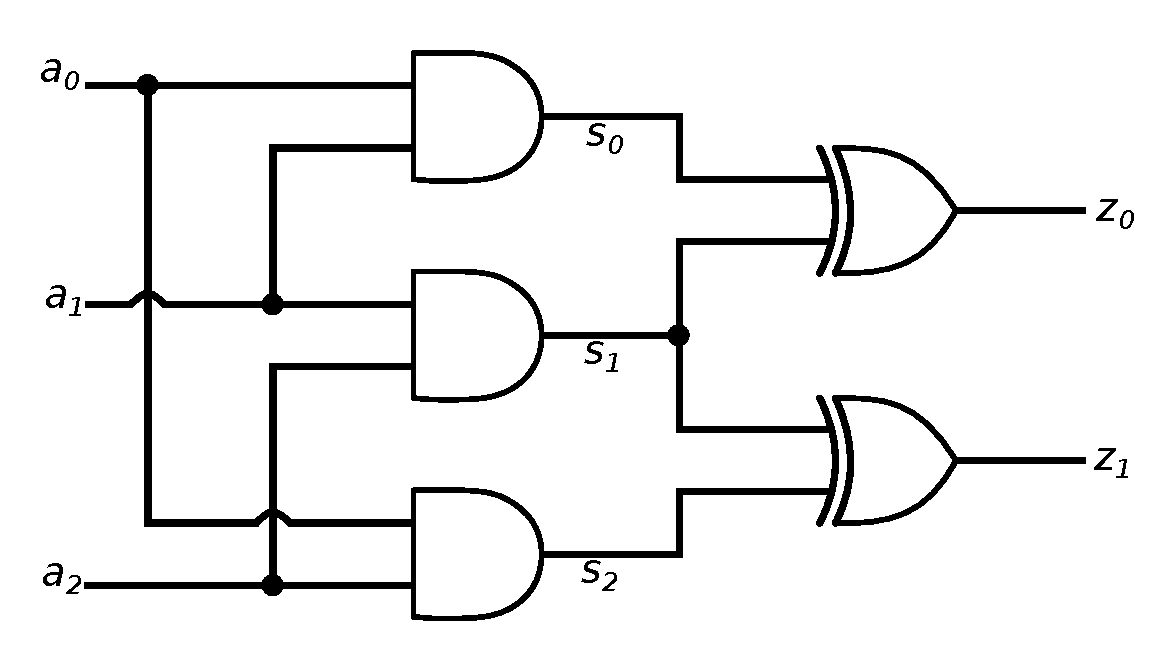
\includegraphics[scale=0.4]{./figures/3to2.eps}
}
\caption{ Circuit with varying word sizes.}
\label{fig:3to2}
\end{figure}
{\it 
Consider the circuit shown in Fig. \ref{fig:3to2}. The input, $A$, is 3 bits 
wide while the output, $Z$ is 2 bits. Thus, $A\in {\mathbb{F}}_{2^3}$ and 
$Z \in {\mathbb{F}}_{2^2}$. Let $\beta$ be the primitive element of 
${\mathbb{F}}_{2^3}$ and $\gamma$ be the primitive element of 
${\mathbb{F}}_{2^2}$, i.e. $A=a_0+a_1\beta+a_2\beta^2$ and $Z=z_0+z_1\gamma$.
Thus, the circuit computes the function ${\mathbb{F}}_{2^3}\rightarrow{\mathbb{F}}_{2^2}$. Since $LCM(2,3)=6$, then $\F_{2^2} \subset \F_{2^6}$ and $\F_{2^3} \subset
\F_{2^6}$. So this function mapped to $\F_{2^6} \rightarrow \F_{2^6}$.
Choose $P(X)=X^6+X+1$ as the irreducible
polynomial to construct $\F_{2^6}$, where $P(\alpha)=0$. Then $\beta$ and
$\gamma$ in can be represented in terms of $\alpha$:
\begin{eqnarray}
\beta=\alpha^{(2^6-1)/(2^3-1)}=\alpha^9 \nonumber \\
\gamma=\alpha^{(2^6-1)/(2^2-1)}=\alpha^{21} 
\end{eqnarray}
So the word-level polynomials are:
\begin{eqnarray}
&&f_A: a_0+a_1\alpha^9+a_2\alpha^{18}+A \nonumber \\
&&f_Z: z_0+z_1\alpha^{21}+Z 
\end{eqnarray}
The rest of the polynomials in $F$ are derived from the circuit:
\begin{eqnarray}
f_1: z_0+s_0+s_1 & f_2: z_1+s_1+s_2 & f_3: s_0+a_0\cdot a_1 \nonumber \\
f_4: s_1+a_1\cdot a_2 & f_5: s_2+a_0\cdot a_2 &
\end{eqnarray}
where the RATO ordering is:
\begin{equation}
z_0 > z_1 > s_0 > s_1 > s_2 > a_0 > a_1 > a_2 > Z > A
\end{equation}
$F_0$ is defined as before, except with a change to the polynomials derived from word-level 
variables $A$ and $Z$:
\begin{eqnarray}
f_6: z_0^2+z_0 & f_7: z_1^2+z_1 & f_8: s_0^2+s_0 \nonumber \\
f_9: s_1^2+s_1 & f_{10}: s_2^2+s_2 & f_{11}: a_0^2+a_0 \nonumber \\
f_{12}: a_1^2+a_2 & f_{13}: a_2^2+a_2 & f_{14}: Z^4+Z \nonumber \\
f_{15}: A^8+A & & 
\end{eqnarray}

Computing $f_Z\xrightarrow{F-{f_z},F_0}_+ r$ gives:
\begin{eqnarray}
r&=& (\alpha^2+\alpha)\cdot a_1\cdot a_2+a_1\cdot A+(\alpha^4+\alpha^3)\cdot a_1 \nonumber \\
&&+(\alpha^5+\alpha^4+\alpha^3+\alpha+1)\cdot a_2\cdot A+(\alpha^5+\alpha^4+\alpha^2+\alpha)\cdot a_2+Z
\end{eqnarray}

This result must be further reduced by $f_{a_1}: a_1 + \Func_{a_1}(A)$ and $f_{a_2}: a_2 + \Func-{a_2}(A)$. 
First, find $\mathbf{M}$ in terms of $\beta$ as derived from $A=a_0+a_1\beta+a_2\beta^2$.
Then map it to $\alpha$.  

\begin{eqnarray}
\mathbf{M}=
\begin{bmatrix}
1      &   \beta   & \beta^2  \\
1      &   \beta^2 & \beta^4  \\
1      &   \beta^4 & \beta^8
\end{bmatrix} & 
\mathbf{M_1}=
\begin{bmatrix}
1      &   A   & \beta^2  \\
1      &   A^2 & \beta^4  \\
1      &   A^4 & \beta^8
\end{bmatrix} &
\mathbf{M_2}=
\begin{bmatrix}
1      &   \beta   & A  \\
1      &   \beta^2 & A^2  \\
1      &   \beta^4 & A^4
\end{bmatrix}
\end{eqnarray}

Computing the determinants in $f_{a_1}: a_1 + |\mathbf{M_1}|$ and $f_{a_2}: a_2 + |\mathbf{M_2}|$ gives:
\begin{eqnarray}
f_{a_1}: a_1+A^4\cdot (\beta^4+\beta^2)+A^2\cdot (\beta^8+\beta^2)+A\cdot (\beta^8+\beta^4) \nonumber \\
f_{a_2}: a_2+A^4\cdot (\beta^2+\beta)+A^2\cdot (\beta^4+\beta)+A\cdot (\beta^4+\beta^2)
\end{eqnarray}
Replacing all $\beta$ in $f_{a_1}$ and $f_{a_2}$ with $\alpha^9$ gives their proper form over $\F_{2^6}$.
\begin{eqnarray}
f_{a_1}: a_1+A^4\cdot(\alpha^4+\alpha^3+1)+A^2\cdot(\alpha^4+\alpha^2+\alpha+1)+A\cdot(\alpha^3+\alpha^2+\alpha) \nonumber \\
f_{a_2}: a_2+A^4\cdot(\alpha^4+\alpha^2+\alpha+1)+A^2\cdot(\alpha^3+\alpha^2+\alpha)+A\cdot(\alpha^4+\alpha^3+1)
\end{eqnarray}

Finally, computing the reduction $r\xrightarrow{f_{a_1},f_{a_2},F_0}_+ r_w$ gives the word-level polynomial
abstraction of the circuit.
%Applying the abstraction approach, the word-level polynomial $Z+\F(A)$ found is

\begin{eqnarray}
r_w:&&Z+A^6(\alpha^2+\alpha)+A^5(\alpha^4+\alpha^3+\alpha)+A^4(\alpha^2+\alpha) \nonumber \\
&&+A^3(\alpha^4+\alpha^3+\alpha^2)+A^2(\alpha^4+\alpha^3+\alpha^2)+A(\alpha^4+\alpha^3+\alpha) \nonumber
\end{eqnarray}
}
\end{Example}

This result allows the abstraction to be computed over fields of different sizes. 
An important application of this result is that of modularly-designed composite 
field arithmetic circuits.
These circuits compute operations over very large fields (i.e. $k=1024$) by combining 
operations over smaller sub-fields (i.e. $k=32$).
The abstraction approach can be efficiently applied to these types of circuits by
exploiting the hierarchy found in these designs.

\section{Composite Field Arithmetic Circuits}

A Galois field multiplier over $\Fkk$ can be composed over the composite field $\F_{(2^m)^n}$ 
where $k=m\cdot n$ \cite{phdpaar:1994}. Similarly to how $\Fkk$ is a $k$-dimensional 
extension of the subfield $\F_2$, $\F_{(2^m)^n}$ is also an $n$-dimensional extension of $\F_{2^m}$.
A {\bf composite field multiplier} lifts the ground field from $\F_2$ to $\F_{2^m}$ and
computes the multiplication over $\Fkk$ as a collection of operations
over $\F_{2^m}$. Thus, a composite field multiplier over $\Fkk$ is composed internally as a
collection of {\it multipliers} and {\it adders} over $\F_{2^m}$.

This hierarchy found in composite field multipliers can be exploited by the proposed 
abstraction approach. Abstraction of these types of multipliers is composed of
two steps:
\begin{enumerate}
\item Compute the canonical word-level polynomial representation of each $\F_{2^m}$ multiplier and adder.
\begin{itemize}
  \item These abstractions are independent of one another. Thus, they are computed in parallel.
  \item In the case of an adder, the abstraction is trivial.
\end{itemize}
\item Compute the overall abstraction of the $\Fkk$ multiplier.
\end{enumerate}
The first step utilizes the proposed abstraction approach over $\F_{2^m}$ with no changes.
Once these word-level abstractions are known, they replace the gate-level
implementations for the final word-level abstraction of the multiplier over $\Fkk$.
%Design of composite field multipliers is explored in Chapter \label{ch:prelim}.

\subsection{Design of Composite Field Multipliers}

The following adapts principles of composite fields from \cite{phdpaar:1994} and 
explains how they are applied to construct Galois field multipliers.
Consider the element $A \in \Fkk$ and its representation over 
$\F_{(2^m)^n}$. Let $\alpha$ be the primitive element of $\Fkk$ and let $\gamma$
be the primitive element of $\F_{(2^m)^n}$. Then any element $A \in \mathbb{F}_{2^k}$ 
is represented as:
\begin{equation}
A=a_0+a_1\alpha+\dots+a_{k-1}\alpha^{k-1},\text{where } a_i  \in \mathbb{F}_{2} \label{eqn:compAf2k}
\end{equation}
This same element $A \in \mathbb{F}_{(2^m)^n}$ is represented as:
\begin{equation}
A=A_0+A_1\gamma+\dots+A_{n-1}\gamma^{n-1},\text{where } A_i \in \mathbb{F}_{2^m} \label{eqn:compAf2m}
\end{equation}
Let $\beta$ be the primitive element of $\F_{2^m}$. Then each $A_i$ is represented as
\begin{equation}
A_i=a_{i0}+a_{i1}\beta+\dots+a_{i\{m-1\}}\beta^{m-1},\text{where } a_{ij}\in\F_2
\end{equation}

Since there always exists a unique field with $p^k$ elements, the field $\Fkk$ is isomorphic to 
the field $\F_{(2^m)^n}$. Due to this, $\gamma = \alpha$. Furthermore, $\beta$ can be derived 
from $\alpha$ using Eqn.(\ref{eqn:betaToAlpha}) since $\F_{2^m} \subset \Fkk$, i.e. 
$\beta=\alpha^w$ for some $w$. Thus, all
that is required to construct a composite field multiplier over $\F_{(2^m)^n}$ is 
the primitive polynomial $P(x)$ which generates $\Fkk$, with $P(\alpha)=0$, 
where $\beta$ is known.

In order to lift the ground field $\F_2$ to $\F_{2^m}$, the variables $\{a_{00},\dots,a_{\{n-1\}\{m-1\}}\}$
must be derived in terms of $\{a_0,\dots,a_{k-1}\}$. Equating the representation of $A\in\Fkk$
with the representation of $A\in\F_{(2^m)^n}$ from Eqns.(\ref{eqn:compAf2k}) and (\ref{eqn:compAf2m}) 
gives the following:
\begin{eqnarray}
& &a_0+a_1\alpha+\dots+a_{k-1}\alpha^{k-1} \nonumber \\
&=&A_0+A_1\alpha+\dots+A_{n-1}\alpha^{n-1} \nonumber \\
&=&\sum_{i=0}^{i=n-1}(\sum_{j=0}^{j=m-1}a_{ij} \cdot \alpha^{wj}) \cdot \alpha^i
\end{eqnarray}
%
Here, every $A_0,\dots,A_{n-1}$ is replaced by its representation over $\F_{2^m}$. Analyzing
the coefficients
gives $\{a_0,\dots,a_{k-1}\}$ in terms of $\{a_{00},\dots,a_{\{n-1\}\{m-1\}}\}$. This mapping can be
depicted as a matrix multiplication.

\begin{equation}
\begin{bmatrix} a_0\\ \vdots \\ a_{k-1}\end{bmatrix}
=\mathbf{T}
\begin{bmatrix} a_{00}\\ \vdots \\ a_{\{n-1\}\{m-1\}}\end{bmatrix}
\end{equation}
where $\mathbf{T}$ is a $k$ by $k$ matrix consisting of elements in $\F_2$. Inverting 
$\mathbf{T}$ gives a mapping from $\{a_{00},\dots,a_{\{n-1\}\{m-1\}}\}$ to $\{a_0,\dots,a_{k-1}\}$.

\begin{Example}\label{ex:comp22}
An example composite field multiplier $\F_{(2^2)^2}$, which computes a multiplication
over $\F_{2^4}$, is shown in Figure \ref{fig:comp4ex}. Notice that, after the transformation,
all additions and multiplications are computed over the base field $\F_{2^2}$.

\begin{figure}[t]
        \centering
        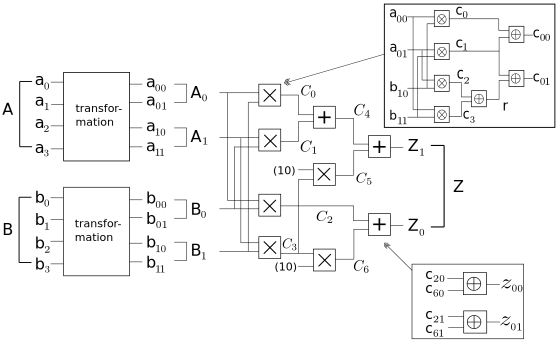
\includegraphics[width=.9\linewidth]{./figures/compMineSmall}
        \caption{$4$-bit composite multiplier designed over $\F_{(2^2)^2}$}\label{fig:comp4ex}
\end{figure}

Let $P(x) = x^4 + x^3 + 1$ and $P(\alpha)=0$. 
Representation of element $A \in \mathbb{F}_{(2^2)^2}$ is:
\begin{eqnarray}
A& = A_0 +A_1 \cdot \alpha
\end{eqnarray}
Representation of $A_0, A_1$ in $\mathbb{F}_{2^m}$ is:
\begin{eqnarray}
A_0=a_{00}+a_{01} \cdot \beta \nonumber \\
A_1=a_{10}+a_{11} \cdot \beta
\end{eqnarray}
where $a_{ij}\in \mathbb{F}_2$. From Eqn.(\ref{eqn:betaToAlpha}), $\beta=\alpha^5$
Now $A_0, A_1$ can be substituted into $A$ as follows:
\begin{eqnarray}
A&=&a_{00}+a_{01}\cdot \alpha^5+(a_{10}+a_{11}\cdot \alpha^5)\cdot \alpha
\end{eqnarray}
Since $P(x)=x^4+x^3+1$ with $P(\alpha)=0$,
\begin{equation}\label{a}
A \pmod {P(\alpha)}=a_{00}+a_{01}+a_{11}+(a_{01}+a_{10}+a_{11})\cdot \alpha+a_{1
1} \cdot \alpha^2+(a_{01}+a_{11})\cdot \alpha^3   
\end{equation}
The same element $A \in \mathbb{F}_{2^4}$ is represented as:
\begin{equation}\label{aa}
A=a_0+a_1\cdot \alpha+a_2\cdot \alpha^2+a_3\cdot \alpha^3 
\end{equation}

\item Since Eqns. (\ref{a}) and (\ref{aa}) represent the same element, we
  can match the coefficients of the the polynomials to obtain:
\begin{eqnarray}
a_0&=&a_{00}+a_{01}+a_{11} \nonumber \\
a_1&=&a_{01}+a_{10}+a_{11} \nonumber \\
a_2&=&a_{11} \nonumber \\
a_3&=&a_{01}+a_{11} \nonumber
\end{eqnarray}

This mapping can also be reversed and represented as a matrix $T^{-1}$:
\begin{equation}
\begin{bmatrix} a_{00}\\ a_{01} \\a_{10} \\ a_{11}\end{bmatrix}
=
\begin{bmatrix} 1 & 0 & 0 & 1\\ 0 & 0 & 1 & 1\\ 0 & 1 & 0 & 1\\ 0 & 0
  & 1 & 0 \end{bmatrix} 
\begin{bmatrix} a_0\\ a_1 \\a_2 \\ a_3\end{bmatrix}
\end{equation}
Thus, $A$ is represented in $\mathbb{F}_{(2^2)^2}$ as:
\begin{eqnarray}
A&=&A_0+A_1 \cdot \alpha \nonumber \\
A_0&=&a_{00}+a_{01} \cdot \alpha^5 \nonumber \\
A_1&=&a_{10}+a_{11} \cdot \alpha^5 \nonumber \\
a_{00}&=&a_0+a_3 \nonumber \\
a_{01}&=&a_2+a_3 \nonumber \\
a_{10}&=&a_1+a_3 \nonumber \\
a_{11}&=&a_2 \nonumber 
\end{eqnarray}
$B$ is similarly represented in $\mathbb{F}_{(2^2)^2}$.
\end{Example}

\subsection{Abstraction of Composite Field Multipliers}

The first step in abstracting the word-level polynomial representation of the composite field
multiplier is to abstract every internal $\F_{2^m}$ computational block. In the case of a $\F_{2^m}$
adder block ($\{Z_0,Z_1,C_4\}$ from Fig.(\ref{fig:comp4ex})), this abstraction is trivial, as the adder is just a bit-wise XOR computation. In the case
of a multiplier block ($\{C_0,C_1,C_2,C_3,C_5,C_6\}$ from Fig.(\ref{fig:comp4ex})), 
the abstraction approach presented in the previous chapter is directly 
applicable. Each abstraction can be computed independently, so these computations can be 
performed in parallel. This set of abstracted polynomials, $F$, generates the ideal $J$.

Once the word-level abstraction of each $\F_{2^m}$ sub-block is known, the final abstraction of the 
entire design can be computed using only word-level variables. Set a RATO ordering. Then
reduce the word level polynomial by $F+F_0$:
\begin{equation}
f_Z: Z_0+Z_1\alpha+\dots+Z_{n-1}\alpha^{n-1}+Z
\end{equation}
\begin{equation}
f_Z\xrightarrow{F+F_0}_+ r
\end{equation}
Here, $F$ is the set of word-level
polynomial abstractions from each $\F_{2^m}$ block and $F_0$ is the set of vanishing polynomials.
Every variable $X$, apart from the word-level inputs $A$ and $B$ and word-level output $Z$, is an element of
$\F_{2^m}$, so its corresponding vanishing polynomial is $X^{2^m}+X$. Computing the reduction
gives remainder $r$ containing the elements 
\begin{equation}
A_0,A_1,\dots,A_{n-1},B_0,B_1,\dots,B_{n-1},Z
\end{equation}
Similarly, the mapping from $\{A_0,\dots,A_{n-1}\}$ to $A$ now needs to be derived (along with
the mapping from $\{B_0,\dots,B_{n-1}\}$ to $B$). That is, the next step is to find 
\begin{eqnarray}
& &F_A=\{F_{A_0},F_{A_1},\dots,F_{A_{n-1}}\} \nonumber \\
\text{where }& &F_{A_i}=A_i+\Func_{A_i}(A)
\end{eqnarray}
$F_A$ is derived from the polynomial
\begin{equation}
A=A_0+A_1\alpha+\dots+A_{n-1}\alpha^{n-1}
\end{equation}
Compute $A^{2^m}$ as follows:
\begin{eqnarray}
A^{2^m}: & & (A_0+A_1\alpha+\dots+A_{n-1}\alpha^{n-1})^{2^m} \nonumber \\
&&=A_0^{2^m}+A_1^{2^m}\alpha^{2^m}+\dots+A_{n-1}^{2^m}\alpha^{2^m(n-1)} \nonumber \\
&&=A_0+A_1\alpha^{2^m}+\dots+A_{n-1}\alpha^{2^m(n-1)}
\end{eqnarray}
Here, the property is $A_i^{2^m}=A_i$ is exploited. Continually raise this result by $2^m$ 
to obtain $A^{2^{jm}}$ for all $0\leq j < n$. This gives a system of $n$ equations and $n$
unknowns $\{A_0,\dots,A_{n-1}\}$. As before, this system of equations can be represented
in matrix form, $\mathbf{A = M a}$, where 
$\mathbf{A}=\{A,A^{2^m},\dots,A^{2^{(n-1)m}}\}^T$, 
$\mathbf{M}$ is
a $n$ by $n$ matrix of coefficients $\in \Fkk$, and $\mathbf{a}=\{A_0,\dots,A_{n-1}\}^T$:

\begin{eqnarray}
\begin{bmatrix}
A \\ A^{2^m} \\ \vdots \\ A^{2^{(n-1)m}}
\end{bmatrix}  &=&
\begin{bmatrix}
1      &   \alpha          & \alpha^2         & \dots & \alpha^{n-1}\\
1      &   \alpha^{2^m}     & \alpha^{2\cdot2^m}    & \dots & \alpha^{(n-1)\cdot 2^m}\\
1      &   \alpha^{2^{2m}}   & \alpha^{2\cdot2^{2m}}    & \dots & \alpha^{(n-1)\cdot 2^{2m}}\\
\vdots & \vdots            & \vdots           & \cdot & \vdots \\
1      &   \alpha^{2^{(n-1)m}} & \alpha^{2\cdot2^{(n-1)m}} & \dots & \alpha^{(n-1)\cdot 2^{(n-1)m}}
\end{bmatrix}
\begin{bmatrix}
A_0 \\ A_1 \\ \vdots \\ A_{n-1}
\end{bmatrix} \label{eqn:matrixForm}
\end{eqnarray}

The matrix $\mathbf{M}$ is the Vandermonde matrix $V(\alpha,\alpha^{2^m},\dots,\alpha^{2^{(n-1)m}})$.
Since $\alpha$ is a primitive element, 
all elements $\alpha,\dots,\alpha^{2^{k-1}}$ are unique, where $k=m\cdot n$. Thus, 
all elements $\alpha,\alpha^{2^m},\dots,\alpha^{2^{(n-1)m}}$ are unique, so
$|\mathbf{M}| \neq 0$. Then, Cramer's rule can be applied to derive each $F_{A_i}$ as 
\begin{equation}
F_{A_i}=A_i+\frac{|\mathbf{M_i}|}{|\mathbf{M}|}
\end{equation}
where $\mathbf{M_i}$ is $\mathbf{M}$ with the $i$-th column replaced
by $\mathbf{A}$. Here, $|\mathbf{M}|$ is not guaranteed to be equal to $1$,  
%Rather, $|\mathbf{M}|$ is a non-zero element of $\F_{2^m}$ (proof in Appendix \ref{append:Fpk}),
so it must be computed. 
$F_B=\{F_{B_0},\dots,F_{B_{n-1}}\}$ is similarly derived.
Computing $r\xrightarrow{F_A,F_B,J_0}_+ r_w$ gives $r_w: Z+\Func(A,B)$ which is the 
canonical word-level polynomial abstraction of the composite field design.

\begin{Example}
Consider the composite field multiplier over $\F_{{2^2}^2}$ from Example \ref{ex:comp22}.
Abstracting every multiplier and adder over the base field $\F_{2^2}$ gives the following
polynomials:
\begin{eqnarray}
f_1: Z_0+C_6+C_2      & f_2: Z_1+C_5+C_4      & f_3: C_6+\alpha^5C_3 \nonumber \\
f_4: C_5+\alpha^5C_3  & f_5: C_4+C_1+C_0      & f_6: C_3+A_1\cdot B_1 \nonumber \\
f_7: C_2+A_0\cdot B_0 & f_8: C_1+A_1\cdot B_0 & f_9: C_0+A_0\cdot B_1 
\end{eqnarray}
Set the following RATO ordering:
\begin{eqnarray}
Z_0 > Z_1 > C_6 > C_5 > C_4 > C_3 > C_2 > C_1 > C_0 \nonumber \\
> A_0 > A_1 > B_0 > B_1 > Z > A > B
\end{eqnarray}
The vanishing polynomials are:
\begin{eqnarray}
f_{10}: Z_0^4+Z_0 & f_{11}: Z_1^4+Z_1 & f_{12}: C_6^4+C_6 \nonumber \\
f_{13}: C_5^4+C_5 & f_{14}: C_4^4+C_4 & f_{15}: C_3^4+C_3 \nonumber \\
f_{16}: C_2^4+C_2 & f_{17}: C_1^4+C_1 & f_{18}: C_0^4+C_0 \nonumber \\
f_{19}: A_0^4+A_0 & f_{20}: A_1^4+A_1 & f_{21}: B_0^4+B_0 \nonumber \\
f_{22}: B_1^4+B_1 & f_{23}: Z^{16}+Z  & f_{24}: A^{16}+A \nonumber \\
f_{25}: B^{16}+B
\end{eqnarray}
Then $F=f_1,\dots,f_9$ and 
$F_0=f_{10},\dots,f_{25}$.
Here, $f_Z: Z_0+Z_1\alpha+Z$. Computing $f_Z\xrightarrow{F,F_0}_+ r$ gives:
\begin{equation}
r= A_0\cdot B_0+\alpha A_0\cdot B_1+\alpha A_1\cdot B_0+\alpha^2A_1\cdot B_1+Z
\end{equation}

Next, $F_A=\{F_{A_0},F_{A_1}\}$ needs to be derived. Here, $A=A_0+A_1\alpha$ and $A^{4}=A_0+A_1\alpha^4$,
which gives
\begin{eqnarray}
\mathbf{M}=
\begin{bmatrix}
1 & \alpha \\
1 & \alpha^4
\end{bmatrix}; &
\mathbf{M_0}=
\begin{bmatrix}
A & \alpha \\
A^4 & \alpha^4
\end{bmatrix}; &
\mathbf{M_1}=
\begin{bmatrix}
1 & A \\
1 & A^4
\end{bmatrix}
\end{eqnarray}
After minimizing by the primitive polynomial $P(x)=x^4+x^3+1$, 
the determinants of these matrices are:
\begin{eqnarray}
|\mathbf{M}|=\alpha^3+\alpha+1; &
|\mathbf{M_0}|=\alpha A^4+(\alpha^3+1)A; &
|\mathbf{M_1}|=A^4+A
\end{eqnarray}
%Notice that $|\mathbf{M}|=\alpha^5=\beta\in\F_{2^2}$.%% NOTE: haven't figured out if this is always the case 
Now $F_{A_0}$ and $F_{A_1}$ are derived:
\begin{eqnarray}
F_{A_0} = &A_0+\frac{|\mathbf{M_0}|}{|\mathbf{M}|}& = A_0+(\alpha^3+\alpha^2+1)A^4+(\alpha^3+\alpha^2)A \\
F_{A_1} = &A_1+\frac{|\mathbf{M_1}|}{|\mathbf{M}|}& = A_1+(\alpha^3+\alpha)A^4+(\alpha^3+\alpha)A
\end{eqnarray}
Since $F_B=\{F_{B_0},F_{B_1}\}$ is derived from $B=B_0+B_1\alpha$, which is isomorphic to
$A=A_0+A_1\alpha$, then $F_B$ can be derived from $F_A$ by substituting corresponding
variables.
\begin{eqnarray}
F_{B_0}& = &B_0+(\alpha^3+\alpha^2+1)B^4+(\alpha^3+\alpha^2)B \\
F_{B_1}& = &B_1+(\alpha^3+\alpha)B^4+(\alpha^3+\alpha)B
\end{eqnarray}
Finally, computing $r\xrightarrow{F_A,F_B,F_0}_+ r_w$ gives the word-level abstraction of
the circuit.
\begin{equation}
r_w: Z+A\cdot B
\end{equation}


\end{Example}

\section{Conclusion}

This chapter described how to generalize the abstraction approach to any arbitrary
combinational circuit. This method works best when the derived operand-width $k$, from the $LCM$ of the 
word-lengths of all inputs and output, is not very large, for instance, when the output size is a 
multiple of the input sizes. When all word-sizes are relatively prime,
$k$ is a product of all sizes, which can make the analysis overly bulky.

An abstraction technique for exploiting the hierarchy of composite field multiplier circuits over
$\F_{(2^m)^n} $
was also examined. The approach abstracts all internal multipliers and adders over $\F_{2^m}$ in 
parallel and uses these abstractions to compute the final abstraction completely over
word-level variables. Experimental results for abstractions of composite field multipliers using a
custom-built tool is presented in the next chapter.

\chapter{Implementation of the Custom Abstraction Software and Experimental Results} \label{ch:implement}

The abstraction procedure can be fully scripted using the computer algebra tool 
{\sc Singular}. However, {\sc Singular} has limitations which make abstraction
of large circuits {\it impossible}. This is due to:
\begin{itemize}
\item A limit on the number of ring variables allowed. As of {\sc Singular} release 4.0.1, 
a ring cannot be declared with more than $32,767$ variables. This limits the number
of gates that can be present in the design.
\item The size of an exponent $(n)$ of a variable $x$, is limited $n<2^{32}$.
\item Large amount of memory usage and slow computation time. 
{\sc Singular} uses a dense-distributive structure for polynomials, which is a poor 
representation of sparse polynomials over rings with many variables.
\end{itemize}
The limit on the size of exponents prohibits an abstraction beyond $32$-bit circuits,
as larger circuits require manipulating word-level variables with exponents 
larger than $2^{32}$. Even
if this limitation is overcome, Singular uses an enormous amount of memory.
For instance, preliminary experiments show that using Singular to compute the
initial reduction of a $163$-bit Mastrovito multiplier uses $41.6$ GB of memory!
Thus, deriving abstractions using Singular is infeasible on 
desktop workstations.

In order to overcome these limitations, a custom C++ tool is developed to 
compute the word-level abstraction of circuits quickly and efficiently. 
This chapter describes the implementation details of this tool.

\section{Data Structures and Algorithms}

Computing a word-level abstraction requires the representation and manipulation 
of polynomials in $\Fkk[x_1,\dots,x_d]$ over a lex ordered ring. 
Intermediate polynomials can become 
very large during the abstraction procedure, so the data structure to represent them 
is designed to 
conserve memory while allowing for fast manipulation during the reduction 
procedures. The backbone of the tool is a custom library composed of three main
sections:
\begin{enumerate}
\item Galois field elements
\item Monomials and rings
\item Polynomials and division procedures
\end{enumerate}
These are built on top of each other. The starting point is the custom 
Galois field element section, which facilitates the construction of 
Galois field elements over $\Fkk$.

\subsection{Galois Field Elements}

The Galois field section of the library is initialized by parsing a given primitive polynomial $P(x)$
of degree $k$ which constructs $\Fkk$. Any element $C \in \Fkk$ can be represented 
in the form 
\begin{equation}
C = c_{k-1}\cdot\alpha^{k-1}+c_{k-2}\cdot\alpha^{k-2}+\cdots+c_2\cdot\alpha^2+c_1\cdot\alpha+c_0
\end{equation}
where 
$\{c_0,\dots,c_{k-1}\}\in\F_2$ and $\alpha$ is the primitive element. This {\it structure}
is stored as an unsigned byte array containing $\{c_0,\dots,c_{k-1}\}$, 
as shown in Figure \ref{fig:gfStruct}. Thus, each element uses $\left\lfloor\frac{k-1}{8}\right\rfloor+1$ 
bytes of memory. 
Any leading bits after $c_{k-1}$ in the last byte are set to $0$.
\begin{figure}[h]
	\begin{center}
	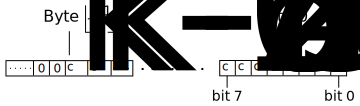
\includegraphics[scale=1]{figures/gfElementStructure}
	\end{center}
	\caption{Object structure of a Galois field element}
	\label{fig:gfStruct}
\end{figure}

{\it Addition} between two elements
\begin{eqnarray}
C&=&c_{k-1}\cdot\alpha^{k-1}+\cdots+c_2\cdot\alpha^2+c_1\cdot\alpha+c_0 \\
D&=&d_{k-1}\cdot\alpha^{k-1}+\cdots+d_2\cdot\alpha^2+d_1\cdot\alpha+d_0
\end{eqnarray}
is simply a combination of like terms
\begin{equation}
C+D=(c_{k-1}+d_{k-1})\cdot\alpha^{k-1}+\cdots+(c_2+d_2)\cdot\alpha^2+(c_1+d_1)\cdot\alpha+(c_0+d_0)
\end{equation}
Since addition over $\F_2$ is computed as a bit-wise XOR, the library's Galois field element 
structure allows addition to be trivially performed as a byte-wise XOR operation. 
Furthermore, this structure makes it easy to check if a given element is equal 
to $0$ or $1$, which is used in deciding when a term is to be removed ($0$) and when 
a division can be ignored ($1$).

During {\it library initialization}, the elements 
$\alpha^k,\alpha^{k+1},\dots,\alpha^{2k-2}$ are pre-computed and cached. First,
$\alpha^k$ is derived directly from the given primitive polynomial, 
\begin{equation}
P(x)=x^k+c_{k-1}\cdot x^{k-1}+\cdots+c_1\cdot x+1
\end{equation}
for $\{c_1,\dots,c_{k-1}\}\in\F_2$. Since $P(\alpha)=0$,
\begin{equation}
\alpha^k=c_{k-1}\cdot\alpha^{k-1}+\cdots+c_1\cdot\alpha+1
\end{equation}
To compute $\alpha^{k+1}$, first compute a $1$-bit left shift of
$\alpha^k$.
\begin{equation}
\alpha^{k+1}=c_{k-1}\cdot\alpha^k+c_{k-2}\cdot\alpha^{k-1}+\cdots+c_1\cdot\alpha^2+\alpha
\end{equation}
This element can contain the term $\alpha^k$, which must be minimized by the primitive
polynomial.
Thus, if $c_{k-1}$ is $1$, the $c_{k-1}\alpha^k$ term is removed and the minimized 
form of $\alpha^k$ is added. This derives the minimized form for $\alpha^{k+1}$. 
Computation continues in this fashion (shift by 1, minimize if needed) until all
$\alpha^k,\alpha^{k+1},\dots,\alpha^{2k-2}$ have been derived.
These elements are later used during the multiplication procedure.

\begin{Example}
\label{ex:gf4init}
Given the primitive polynomial $P(x)=x^4+x^3+1$, initialize the library by computing
$\alpha^4,\alpha^5,$ and $\alpha^6$. Here, $k=4$, and each element of $\F_{2^4}$ can be 
represented as
\begin{equation}
c_3\cdot\alpha^3+c_2\cdot\alpha^2+c_1\cdot\alpha+c_0
\end{equation}
which is stored as one byte in the following form.
\begin{equation}
\begin{tabular}{|c|c|c|c|c|c|c|c|} 
\hline
$0$ & $0$ & $0$ & $0$ & $\mathbf{c_3}$ & $\mathbf{c_2}$ & $\mathbf{c_1}$ & $\mathbf{c_0}$ \\
\hline
\end{tabular}
\end{equation}
Notice that there are $4$ leading bits which are unused; these are always set to $0$.

$P(\alpha)=\alpha^4+\alpha^3+1=0$. Hence, $\alpha^4=\alpha^3+1$, 
which is stored as
\begin{equation}
\begin{tabular}{cc|c|c|c|c|c|c|c|c|} 
\multicolumn{6}{c}{}&\multicolumn{1}{c}{$c_3$}&\multicolumn{1}{c}{$c_2$}&\multicolumn{1}{c}{$c_1$}&\multicolumn{1}{c}{$c_0$} \\
\hhline{~~--------}
$\alpha^4$&$=$&$0$ & $0$ & $0$ & $0$ & $\mathbf{1}$ & $\mathbf{0}$ & $\mathbf{0}$ & $\mathbf{1}$ \\
\hhline{~~--------}
\end{tabular}
\end{equation}
To compute $\alpha^5$, take the $\alpha^4$ element and
shift the result left 1 bit. The $c_3$ term is dropped since the leading $4$ 
bits are always $0$.
\begin{equation}
\begin{tabular}{|c|c|c|c|c|c|c|c|} 
\hline
$0$ & $0$ & $0$ & $0$ & $\mathbf{0}$ & $\mathbf{0}$ & $\mathbf{1}$ & $\mathbf{0}$ \\
\hline
\end{tabular}
\end{equation}

Then, since $c_3$ was $1$, add $\alpha^4$.
\begin{equation}
\begin{tabular}{c|c|c|c|c|c|c|c|c|} 
\hhline{~--------}
&$0$ & $0$ & $0$ & $0$ & $\mathbf{0}$ & $\mathbf{0}$ & $\mathbf{1}$ & $\mathbf{0}$ \\
\hhline{~========}
$+$&$0$ & $0$ & $0$ & $0$ & $\mathbf{1}$ & $\mathbf{0}$ & $\mathbf{0}$ & $\mathbf{1}$ \\
\hhline{~--------}\multicolumn{9}{c}{}\\
\hhline{---------}\multicolumn{9}{c}{}\\
\hhline{~--------}
&$0$ & $0$ & $0$ & $0$ & $\mathbf{1}$ & $\mathbf{0}$ & $\mathbf{1}$ & $\mathbf{1}$ \\
\hhline{~--------}
\end{tabular}
\end{equation}
This gives $\alpha^5=\alpha^3+\alpha+1$. Similarly, $\alpha^6$ is derived as
\begin{equation}
\begin{tabular}{c|c|c|c|c|c|c|c|c|} 
\hhline{~--------}
&$0$ & $0$ & $0$ & $0$ & $\mathbf{0}$ & $\mathbf{1}$ & $\mathbf{1}$ & $\mathbf{0}$ \\
\hhline{~========}
$+$&$0$ & $0$ & $0$ & $0$ & $\mathbf{1}$ & $\mathbf{0}$ & $\mathbf{0}$ & $\mathbf{1}$ \\
\hhline{~--------}\multicolumn{9}{c}{}\\
\hhline{---------}\multicolumn{9}{c}{}\\
\hhline{~--------}
&$0$ & $0$ & $0$ & $0$ & $\mathbf{1}$ & $\mathbf{1}$ & $\mathbf{1}$ & $\mathbf{1}$ \\
\hhline{~--------}
\end{tabular}
\end{equation}
\end{Example}

{\it Multiplication} requires temporarily increasing the size of the byte-array to 
store the intermediate result, which can have values up to $\alpha^{2(k-1)}$.
\begin{equation}
c_{2k-2}\cdot\alpha^{2k-2}+\cdots+c_k\cdot\alpha^k+c_{k-1}\cdot\alpha^{k-1}+\cdots+c_2\cdot\alpha^2+c_1\cdot\alpha+c_0
\end{equation}
This result needs to be divided by the given minimum polynomial. Each $\alpha$ 
term with an exponent of $k$ or larger is replaced by its minimized equivalent,
which was computed during initialization. That is, for $i\geq k$, each term for which $c_{i}=1$ 
is removed and the minimized form of $\alpha^i$ added in.

\begin{Example}
\label{ex:gf4mult}
Consider again the setup for $\F_{2^4}$ from Example \ref{ex:gf4init}. Compute the
product of the following two elements:
\begin{eqnarray}
\alpha^3+\alpha^2+1 \\
\alpha^2+\alpha
\end{eqnarray}
These elements are stored respectively as
\begin{eqnarray}
\begin{tabular}{|c|c|c|c|c|c|c|c|} 
\hline
$0$ & $0$ & $0$ & $0$ & $\mathbf{1}$ & $\mathbf{1}$ & $\mathbf{0}$ & $\mathbf{1}$ \\
\hline
\end{tabular} \\
\begin{tabular}{|c|c|c|c|c|c|c|c|} 
\hline
$0$ & $0$ & $0$ & $0$ & $\mathbf{0}$ & $\mathbf{1}$ & $\mathbf{1}$ & $\mathbf{0}$ \\
\hline
\end{tabular}
\end{eqnarray}
The intermediate result is computed using the basic shift-and-add procedure.
\begin{equation}
\begin{tabular}{|c|c|c|c|c|c|c|c|}
\hhline{~~~~----}
\multicolumn{3}{c}{} & & $1$ & $1$ & $0$ & $1$ \\
\hhline{~~~~----}
\multicolumn{3}{c}{} & x & $0$ & $1$ & $1$ & $0$ \\
\hhline{~~~~----}\multicolumn{8}{c}{}\\
\hhline{--------}\multicolumn{8}{c}{}\\
\hhline{~~~~----}
\multicolumn{3}{c}{} & & $0$ & $0$ & $0$ & $0$ \\
\hhline{~~~-----}
\multicolumn{2}{c}{} & & $1$ & $1$ & $0$ & $1$ & \multicolumn{1}{c}{} \\
\hhline{~~-----~}
\multicolumn{1}{c}{} & & $1$ & $1$ & $0$ & $1$ & \multicolumn{2}{c}{} \\
\hhline{~-----~~}
\multicolumn{1}{c|}{$+$} & $0$ & $0$ & $0$ & $0$ & \multicolumn{3}{c}{} \\
\hhline{~----~~~}\multicolumn{8}{c}{}\\
\hhline{--------}\multicolumn{8}{c}{}\\
\hhline{--------}
$0$& $\mathbf{0}$ & $\mathbf{1}$ & $\mathbf{0}$ & $\mathbf{1}$ & $\mathbf{1}$ & $\mathbf{1}$ & $\mathbf{0}$ \\
\hline
\end{tabular}
\end{equation}
The intermediate result of the multiplication is $\alpha^5+\alpha^3+\alpha^2+\alpha$, 
which needs to be further minimized. The value of $\alpha^5$ was determined during
initialization to be $\alpha^3+\alpha+1$. The $\alpha^5$ term from the intermediate
result is removed and the minimized form is added.

\begin{equation}
\begin{tabular}{cc|c|c|c|c|c|c|c|c|} 
\hhline{~~--------}
&&$0$ & $0$ & $0$ & $0$ & $\mathbf{1}$ & $\mathbf{1}$ & $\mathbf{1}$ & $\mathbf{0}$ \\
\hhline{~~========}
&$+$&$0$ & $0$ & $0$ & $0$ & $\mathbf{1}$ & $\mathbf{0}$ & $\mathbf{1}$ & $\mathbf{1}$ \\
\hhline{~~--------}\\
\hhline{----------}\\
\hhline{~~--------}
&&$0$ & $0$ & $0$ & $0$ & $\mathbf{0}$ & $\mathbf{1}$ & $\mathbf{0}$ & $\mathbf{1}$ \\
\hhline{~~--------}
\end{tabular}
\end{equation}

So the minimized result of the product is $\alpha^2+1$.

\end{Example}

{\it Division} of two Galois field elements, $C=\frac{B}{A}$, requires finding 
the multiplicative inverse of the divisor: $C=B\cdot A^{-1}$. To find the inverse, 
the library implements the extended Euclidean algorithm over $\Fkk$, depicted in
Algorithm \ref{alg:eucInv}. The algorithm requires a non-minimized 
representation of the element $P(\alpha)$, so the size of object is temporarily 
increased to allow the storage of the $\alpha^k$ bit.
The function $DIV$ returns the quotient and 
remainder of a Euclidean division; that is, $DIV(A,B)$ returns 
$\{Q,R\}$, where $A=B\cdot Q + R$. This procedure is described in Algorithm \ref{alg:eucDiv};
here, $DEG$ returns the highest degree of a given element in $\Fkk$, 
i.e. $DEG(\alpha^4+\alpha^3+1)$ would return $4$.

\begin{algorithm}[hbt]
\SetAlgoNoLine

 \KwIn{$M:=P(\alpha)$ where $P(x)$ was used to generate $\Fkk$, $A\in\Fkk$}
 \KwOut{$A^{-1}$ over $\Fkk$}
  %%%%%%%%%%%%%%%%%%%%
        $\{Q_0,Q_1\}$ := $\{0,0\}$\;
        $\{R_0,R_1\}$ := $\{M,A\}$\;
        $\{U_0,U_1\}$ := $\{0,1\}$\;
        $i$ := $1$\;
        \While { $R_i \neq 1$ }
        {
                \If { $R_i == 0$ }{{\bf ERROR}: No inverse exists}
                $\{Q_{i+1},R_{i+1}\} := DIV(R_{i-1},R_i)$\;
                $U_{i+1}$ := $(Q_{i+1} \cdot U_i) + U_{i-1}$\;
                $i$ := $i+1$\;
        }
        \Return $U_i$\;
\caption{Inverse of an element over $\Fkk$}\label{alg:eucInv}
\end{algorithm}

\begin{algorithm}[hbt]
\SetAlgoNoLine

 \KwIn{$A,B \in \Fkk$}
 \KwOut{$\{Q,R\}$ such that $A = B\cdot Q + R$}
        $\{Q, R\} := \{0,A\}$\;
        %$d := DEG(B)$\;
        \While { $DEG(R) \geq DEG(B)$ }
        {
                $S$ := $\alpha^{DEG(R)-DEG(B)}$\;
                $Q$ := $Q + S$\;
                $R$ := $R + S\cdot B$\;
        }
        \Return $\{Q,R\}$\;
\caption{$DIV$ (Euclidean Division over $\Fkk$)}\label{alg:eucDiv}
\end{algorithm}

\begin{Example}
Given $P(x)=x^8+x^4+x^3+x+1$ which generates $\F_{2^8}$, find $A^{-1}$ where
$A=\alpha^6+\alpha^4+\alpha+1$. Table \ref{tab:divExTab} shows the steps 
Algorithm \ref{alg:eucDiv} goes through to find the inverse.

\begin{table}[h]
\begin{center}
\caption{Steps to derive the inverse of $\alpha^6+\alpha^4+\alpha+1$ }
\label{tab:divExTab}
%\noindent\resizebox{\textwidth}{!}{%
\begin{tabular}{|c|l|l|l|} 
\hline
$\mathbf{i}$ & \multicolumn{1}{c|}{$\mathbf{Q_i}$} & \multicolumn{1}{c|}{$\mathbf{R_i}$} & \multicolumn{1}{c|}{$\mathbf{U_i}$} \\
\hline
$0$ & $0$                 & $\alpha^8+\alpha^4+\alpha^3+\alpha+1$ & $0$                                 \\
\hline
$1$ & $0$                 & $\alpha^6+\alpha^4+\alpha+1$          & $1$                                 \\
\hline
$2$ & $\alpha^2+1$        & $\alpha^2$                            & $\alpha^2+1$                        \\
\hline
$3$ & $\alpha^4+\alpha^2$ & $\alpha+1$                            & $\alpha^6+\alpha^2+1$               \\
\hline
$4$ & $\alpha$            & $1$                                   & $\alpha^7+\alpha^6+\alpha^3+\alpha$ \\
\hline
\end{tabular}
%}
\end{center}
\end{table}

The derived inverse is $A^{-1}=\alpha^7+\alpha^6+\alpha^3+\alpha$. Correctness
can be checked by computing $A \cdot A^{-1}$ and verifying that the result is $1$.
\end{Example}

\subsection{Rings and Monomials over Galois Fields}

A monomial $M$ over the ring $\Fkk[x_1,\dots,x_d]$ is a power-product of variables from 
the ring along with a coefficient $C \in \Fkk$.
\begin{equation}
M = C \cdot {x_1}^{e_1} \cdot {x_2}^{e_2} \cdots {x_d}^{e_d}; \quad e_i \geq 0
\end{equation}
Ring variables can either be bit-level (representing a single wire within a circuit) or 
word-level (representing a word input or output).
If $x_i$ is a bit-level variable then $x_i \in \F_2$; thus it has the property 
$x_i^2=x_i$, so its exponent $e_i \in \{0,1\}$. 
If the variable is word-level, then $e_i < 2^k$ due to the property $x_i^{2^k}=x_i$.

Lex ordering is the only monomial ordering used for abstraction, and hence it is
the only ordering implemented in the tool. Ring variables are added as strings,
one at a time, along with an argument stating whether the variable is bit-level
or word-level. Each variable is given a unique unsigned integer id, which is 
continuously incremented with each added variable. Thus, ids of two variables 
can be compared to quickly distinguish which variable appears earlier in the 
ordering.

Three static objects are created during initialization of the 
ring:
\bi
\item {\bf strToId} - a map of each variable name (string) to its id (unsigned int)
\item {\bf idToStr} - a map of each id (unsigned int) to its variable name (string)
\item {\bf wordSet} - a set of ids (unsigned int) of all variables which are word-level
\ei
Here, ``map'' and ``set'' are classes of the standard C++ library.
It's important to note that a C++ ``set'' is a container of unique, ordered 
elements (this property is exploited later).
The ``strToId'' map object
is used when constructing monomials to quickly find the id of a parsed variable 
name. The ``idToStr'' map object allows a monomial object to be printed to
the user. The ``wordSet'' object is used to quickly check whether a given variable
is word-level, which determines how it is handled during monomial operations.

Once the ring has been initialized, monomials can be generated and manipulated.
Internally, all monomial variables are manipulated using their ids. 
Each monomial object contains the following:
\bi
\item {\bf coef} - a Galois field object (as described in the previous subsection)
\item {\bf idSet} - a set of ids (unsigned int) of all variables in the monomial
\item {\bf idToExp} - a map of variable ids (unsigned int) to their exponents (BigUnsigned)
\ei
During monomial creation, string variable names are parsed and mapped to their 
corresponding ids, which are then added to the set.
The exponent map is only filled for variables that are word-level. As most 
variables are bit-level in a circuit, most monomials will have a completely empty
map. Since exponents can be much larger than what can be stored in a primitive 
data structure, each exponent is stored as a BigUnsigned object of the open 
source library {\it BigInt} \cite{BigInt}. This is a library which provides
basic functionality for signed and unsigned integers of unbounded size.

{\it Monomial comparison} is required for proper monomial ordering, which is
necessary for implementation of polynomial procedures such as reduction.
The comparison procedure compares the id sets of two monomials, one variable at 
a time. If the variables differ, the smaller id appears earlier in the ordering.
If they are the same, exponents are checked if the variable is word-level. 
This procedure is shown in Algorithm \ref{alg:monComp}.

\begin{algorithm}[hbt]
\SetAlgoNoLine

\KwIn{Monomials $M_1$ and $M_2$}
\KwOut{$<0$ if $M_2>M_1$, $>0$ if $M_1>M_2$, $0$ if $M_1==M_2$}
    id$_1$ := $M_1$.idSet.begin()\;
    id$_2$ := $M_2$.idSet.begin()\;
    \While{id$_1 \neq \varnothing$ $\&\&$ id$_2 \neq \varnothing$}
    {
        \If{id$_1 \neq$ id$_2$}
        {
            \Return id$_2$-id$_1$\;
        }
        \If{id$_1 \in $ wordSet}
        {
            \If{$M_1$.idToExp[id$_1$] $\neq$ $M_2$.idToExp[id$_2$]}
            {
                \Return $M_1$.idToExp[id$_1$] - $M_2$.idToExp[id$_2$]\;
            }
        }
        id$_1$ := $M_1$.idSet.next()\;
        id$_2$ := $M_2$.idSet.next()\;
    }
    \If{id$_1$ == $\varnothing$ $\&\&$ id$_2$ == $\varnothing$}{\Return $0$\;}
    \If{id$_1$ == $\varnothing$}{\Return $-1$\;}
    \Return $1$\;
\caption{Monomial Comparison}\label{alg:monComp}

\end{algorithm}
%\begin{enumerate}
%\item Compare the current ids.
%\begin{enumerate}
%\item If they are different, monomial with the smaller id appears earlier.
%\end{enumerate}
%\item If the current id is word-level, compare exponents.
%\begin{enumerate}
%\item If they are different, monomial with the greater exponent appears earlier.
%\end{enumerate}
%\item Continue to next id in each set.
%\begin{enumerate}
%\item If exactly one set has runs out of ids, the other monomial appears earlier.
%\item If both sets have run out of ids, the monomials are equal.
%\item Otherwise, go back to Step 1.
%\end{enumerate}
%\end{enumerate}

{\it Multiplication} of two monomials is the main function of this portion of
the tool. First, the two Galois field objects are multiplied together using the previously described
method. Then, the two sets of ids are merged together. Since sets can only 
contain unique values, duplicates are discarded; this is done automatically using
the standard set::insert operation. 
%Note that if a monomial is squared, this operation can be ignored.
In the common case, both 
monomials only contain bit-level variables and the multiplication would be
complete. If there are word-level variables in the monomials, the mapped 
exponents of each such variable would be added together and then minimized if the
resulting exponent is $\geq2^k$.

\begin{Example}
\label{ex:gf4MonMult}
Consider again the setup for $\F_{2^4}$ from Example \ref{ex:gf4init}.
Construct the ring $\F_{2^4}[a,b,c,Z]$ with the lex ordering 
$a > b > c > Z$, where $\{a,b,c\}$ are bit-level variables and $Z$ is a 
word-level variable. The initialized monomial static library objects are:
\begin{equation}
\begin{tabular}{lcrc|clcrc|cc} 
\multicolumn{3}{c}{\bf strToId} & & & \multicolumn{3}{c}{\bf idToStr} & & & {\bf wordSet} \\
\hline
``$a$'' & $\rightarrow$ & $0$ & & & $0$ & $\rightarrow$ & ``$a$'' & & & \\
``$b$'' & $\rightarrow$ & $1$ & & & $1$ & $\rightarrow$ & ``$b$'' & & & $\{3\}$\\
``$c$'' & $\rightarrow$ & $2$ & & & $2$ & $\rightarrow$ & ``$c$'' & & & \\
``$Z$'' & $\rightarrow$ & $3$ & & & $3$ & $\rightarrow$ & ``$Z$'' & & &
\end{tabular}
\end{equation}
Let $M_1$ and $M_2$ be the following monomials:
\begin{eqnarray}
M_1=(\alpha^3+\alpha^2+1)a b Z^{10} & & M_2=(\alpha^2+\alpha) b c Z^7
\end{eqnarray}
These are stored internally by the tool as:
\begin{equation}
\begin{tabular}{|c|c|c|c|c|c|c|c|cccc} 
\multicolumn{12}{c}{$\mathbf{M_1}$} \\
\multicolumn{8}{c}{\bf coef} & & {\bf idSet} & & {\bf idToExp}\\
\hhline{--------~~~~}
$0$ & $0$ & $0$ & $0$ & $\mathbf{1}$ & $\mathbf{1}$ & $\mathbf{0}$ & $\mathbf{1}$ & & $\{0, 1, 3\}$ & & $3 \rightarrow 10$ \\
\hhline{--------~~~~}
\multicolumn{12}{c}{}\\
\end{tabular}
\end{equation}
\begin{equation}
\begin{tabular}{|c|c|c|c|c|c|c|c|cccc} 
\multicolumn{12}{c}{$\mathbf{M_2}$} \\
\multicolumn{8}{c}{\bf coef} & & {\bf idSet} & & {\bf idToExp}\\
\hhline{--------~~~~}
$0$ & $0$ & $0$ & $0$ & $\mathbf{0}$ & $\mathbf{1}$ & $\mathbf{1}$ & $\mathbf{0}$ & & $\{1, 2, 3\}$ & & $3 \rightarrow 7$ \\
\hhline{--------~~~~}
\end{tabular}
\end{equation}
It's easy to see that $M_1 > M_2$ in the given ordering, since the 
first element of ``idSet'' in $M_1$ is $0$ while in $M_2$ it is $1$.
Multiplying $M_1$ by $M_2$ is computed by first multiplying the Galois field 
elements (coef) together (as shown in Example \ref{ex:gf4mult}). Then, the two
sets (idSet) are merged (union). 
Notice that, although variable $b$ appears in both monomials, $b^2=b$ due to it
being a bit-level variable. This is handled automatically by the set class 
(duplicates thrown out).
Finally, the two corresponding exponents of variable $Z$ (idToExp) are added together. 
Since this new exponent of $Z$ is $17$, and $17\geq 2^4$, the exponent is 
minimized by the property $Z^{16}=Z$. Thus, the new exponent of $Z$ is $2$.
\begin{equation}
\begin{tabular}{|c|c|c|c|c|c|c|c|cccc} 
\multicolumn{12}{c}{$\mathbf{M_1}\cdot\mathbf{M_2}$} \\
\multicolumn{8}{c}{\bf coef} & & {\bf idSet} & & {\bf idToExp}\\
\hhline{--------~~~~}
$0$ & $0$ & $0$ & $0$ & $\mathbf{0}$ & $\mathbf{1}$ & $\mathbf{0}$ & $\mathbf{1}$ & & $\{0, 1, 2, 3\}$ & & $3 \rightarrow 2$ \\
\hhline{--------~~~~}
\end{tabular}
\end{equation}
So $M_1\cdot M_2 = (\alpha^2+1) a b c Z^2$
\end{Example}

{\it Monomial division} is a procedure mainly used during polynomial reduction. 
Given two monomials 
$M_1$ and $M_2$, compute $\frac{M_1}{M_2}$. That is, find a monomial $M_3$ 
such that $M_1 = M_2 \cdot M_3$.
Monomial division is described in Algorithm \ref{alg:monDiv}. The 
division procedure loops over all variables in $M_2$ and removes them from $M_1$ 
if they are bit-level.
For word-level variables, exponents are subtracted from each other.
If a variable exists in $M_2$ but not in $M_1$, or if the exponent of a 
word-level variable in $M_2$ is larger than in $M_1$, the division is $0$.
Finally at the end, the Galois field elements are divided by each other.

\begin{algorithm}[hbt]
\SetAlgoNoLine

 \KwIn{Monomials $M_1$ and $M_2$}
 \KwOut{$\frac{M_1}{M_2}$ if it exists}
        $M_3$ := $M_1$\;
        \ForEach{id $\in M_2$.idSet}
        {
            \If{id $\notin M_3$ }{\Return NULL\;}
            \eIf{id $\notin$ wordSet}
            {
                $M_3$.idSet.erase(id)\;
            }
            {
                \If{$M_2$.idToExp[id] $> M_3$.idToExp[id]}
                {
                    \Return NULL\;
                }
                $M_3$.idToExp[id] -= $M_2$.idToExp[id]\;
                \If{ $M_3$.idToExp[id] == $0$}{$M_3$.idSet.erase(id)\;}
            }
        }
        $M_3$.coef /= $M_2$.coef\;
        \Return $M_3$\;
\caption{Monomial Division}\label{alg:monDiv}
\end{algorithm}

\subsection{Polynomials and Polynomial Division}
With the monomial structure defined, a polynomial is simply a C++ vector of
monomial objects. These monomial objects are ordered by the given ring ordering,
which is imposed at all times, using monomial comparisons.

{\it Polynomial addition} is computed by simply merging the vector lists of two 
polynomials together, since the two polynomial vectors are already sorted. If two 
monomials are found to be equal, their Galois field coefficients are added 
together and the resulting monomial added to the sum if the new coefficient is 
not $0$.

{\it Multiplication of a polynomial by a monomial}, $P_2 = M_1 \cdot P_1$ is 
detailed in Algorithm \ref{alg:monPolyMult}. Each monomial in $P_1$ is 
iteratively multiplied by $M_1$ to derive a temporary monomial $M_{temp}$, 
which is added to $P_2$. 
Let $M_{last}$ denote the last monomial in $P_2$ at any given time. 
Due to the ordering, typically $M_{last}\geq M_{temp}$ during the procedure.
In cases where it is not, which only happens when exponents have been minimized, 
$M_{temp}$ falls not far earlier than $M_{last}$.
Thus, to add $M_{temp}$ to $P_2$, $M_{temp}$ is compared to monomials in $P_2$ 
in reverse order.
\begin{algorithm}[hbt]
\SetAlgoNoLine

 \KwIn{Monomial $M_1$, Polynomial $P_1$.}
 \KwOut{$M_1 \cdot P_1$}
        $P_2$ := $\varnothing$\;
        \ForEach{Monomial $M_p \in P_1$}
        {
            $M_{temp}$ := $M_p \cdot M_1$\;
            \ForEach{Monomial $M_{p2} \in P_2$ in reverse order}
            {
                \If{$M_{p2} > M_{temp}$}
                {
                    $P_2$.insertAfter($M_{p2}$,$M_{temp}$)\;
                    break\;
                }
                \If{$M_{p2} == M_{temp}$}
                {
                    $M_{p2}$.coef += $M_{temp}$.coef\;
                    \If{$M_{p2}$.coef == $0$}{$P_2$.pop()\;}
                    break\;
                }
            }
            \If{$M_{temp}$ hasn't been inserted}
            {
                $P_2$.insertToFront($M_{temp}$)\;
            }
        }
        \Return $P_2$\;
\caption{Multiplication of a Polynomial by a Monomial}\label{alg:monPolyMult}
\end{algorithm}


{\it Multiplication of polynomials}, $P_3 = P_1 \cdot P_2$, is computed as
numerous monomial-by-polynomial multiplications. Each monomial in $P_1$
is multiplied by the entire polynomial $P_2$ to derive a temporary polynomial
$P_{temp}$. Then, $P_{temp}$ is added to a growing $P_3$. Order is maintained
by these sub-procedures, so no further ordering logic is needed.

\begin{Example}
\label{ex:polyMultAdd}
Assume the environment has been set up over the ring $\F_{2^4}[a,b,c,Z]$ as in
Example \ref{ex:gf4MonMult}. Let $P_1$ and $P_2$ be the following polynomials
\begin{eqnarray}
P_1=(\alpha) ab +bZ^3 && P_2=abc+ab+b
\end{eqnarray}
$P_1+P_2$ is computed by merging the polynomials together. Two monomials exist
with the same order, $(\alpha) a b$ in $P_1$ and $ab$ in $P_2$, so here only the
coefficients are merged.
\begin{equation}
P_1+P_2 = abc + (\alpha+1)ab + bZ^3+b
\end{equation}
$P_1 \cdot P_2$ is computed by taking each monomial of $P_1$ and multiplying it
by $P_2$. The first temporary polynomial generated is:
\begin{equation}
(\alpha)ab \cdot P_2 = (\alpha)ab \cdot (abc+ab+b) = (\alpha)abc+(\alpha)ab+(\alpha)ab=(\alpha)abc
\end{equation}
Notice that, since two equivalent terms were generated, their coefficients were
added together creating $(0)\cdot ab$, so this term was removed. The second
multiplication is
\begin{equation}
bZ^3 \cdot P_2 = bZ^3\cdot(abc+ab+b) = abcZ^3+abZ^3+bZ^3
\end{equation}
Finally, these two polynomials are added together to obtain the final result.
\begin{equation}
P_1\cdot P_2 = abcZ^3+(\alpha)abc+abZ^3+bZ^3
\end{equation}
\end{Example}

{\it Polynomial reduction} is the main procedure computed by the abstraction tool.
To reduce a polynomial $P_1$ by polynomial $P_2$, one reduction step
is computed as
\begin{equation}
P_1\stackrel{P_2}{\textstyle\longrightarrow} P_1 + \frac{LT(P_1)}{LT(P_2)} \cdot P_2
\end{equation}
where $LT$ is the first monomial object of the given polynomial. $\frac{LT(P_1)}{LT(P_2)} P_2$ 
modifies $P_2$ so that it has the same leading term as $P_1$. Thus, when the two 
polynomials are added together, the leading terms are cancelled out. Note that reduction
is only possible when $LT(P_1)$ is divisible by $LT(P_2)$.
However, one reduction step
may not be sufficient to compute a full reduction, i.e. it's possible that the 
resulting polynomial could be reduced further by $P_2$. 
One can reapply the reduction steps until no more reductions are possible.
A more efficient method is to collect all monomials in $P_1$ that are divisible
by $LT(P_2)$, add the results of each division to $P_{temp}$, and then compute
$P_1+P_{temp}\cdot P_2$. 
Due to the ordering, if $LT(P_2) > M_i$ where $M_i$ is the $i^{th}$ monomial in $P_1$, 
then all $M_j \in P_1$ for $j \geq i$ are not divisible by $LT(P_2)$. 
Thus, the divisions are performed in monomial order 
and stopped as soon as this condition holds. The overall procedure is described in 
Algorithm \ref{alg:polyReduction}. Polynomial reduction makes use of 
monomial division, monomial-by-polynomial multiplication,
and polynomial addition, which were all detailed previously.

\begin{algorithm}[hbt]
\SetAlgoNoLine
 \KwIn{Polynomial $P_1$, Polynomial $P_2$.}
 \KwOut{$r$ where $P_1\stackrel{P_2}{\textstyle\longrightarrow}_+ r$}
        $P_{temp}$ := $\varnothing$\;
        \ForEach{Monomial $M_p \in P_1$}
        {
            \If{ $LT(P_2) > M_p$ }
            {
                break\;
            }
            $M_{div}$ := $M_p / LT(P_2)$\;
            \If{ $M_{div}$ $!=$ $\varnothing$ }
            {
                $P_{temp}$.push\_back($M_{div}$)\;
            }
        }
        \Return $P_1 + (P_{temp} \cdot P_2)$\;
\caption{Polynomial Reduction}\label{alg:polyReduction}
\end{algorithm}

\begin{Example}
Consider again the $\F_{2^4}[a,b,c,Z]$ setup from Example \ref{ex:polyMultAdd} 
with
\begin{eqnarray}
P_1=(\alpha) ab +bZ^3 && P_2=abc+ab+b
\end{eqnarray}
Compute $P_2\stackrel{P_1}{\textstyle\longrightarrow}_+ r$. Attempt to divide 
each monomial of $P_2$ by $LT(P_1)=(\alpha)ab$.
The first monomial
division is:
\begin{equation}
\frac{abc}{(\alpha)ab} = (\alpha^3+\alpha^2)c
\end{equation}
Note that over this field, $(\alpha)^{-1}=(\alpha^3+\alpha^2)$.
The next monomial division is:
\begin{equation}
\frac{ab}{(\alpha)ab} = (\alpha^3+\alpha^2)
\end{equation}
The last monomial division is not possible,
\begin{equation}
\frac{b}{(\alpha)ab} = \varnothing
\end{equation}
so $P_{temp}=(\alpha^3+\alpha^2)c+(\alpha^3+\alpha^2)$. The final reduction
is then computed as
\begin{eqnarray}
&&P_2 + (P_{temp} \cdot P_1) \nonumber \\
&&= abc+ab+c+((\alpha^3+\alpha^2)c+(\alpha^3+\alpha^2))\cdot((\alpha) ab +bZ^3) \nonumber \\
&&=abc+ab+c+(abc+ab+(\alpha^3+\alpha^2)bcZ^3+(\alpha^3+\alpha^2)bZ^3) \nonumber \\
&&=(\alpha^3+\alpha^2)bcZ^3+(\alpha^3+\alpha^2)bZ^3+c 
\end{eqnarray}
Notice that the two monomials of $P_2$ that were divisible by $LT(P_1)$ are 
cancelled out.
\end{Example}

\section{Abstraction Tool Flow and Results}

The tool takes the circuit as input
and applies the approach presented in Chapter \ref{ch:improv}
to derive the polynomial representation of the circuit.
The most computationally intensive procedures in the approach are
\begin{enumerate}
\item Initial reduction of the word-level polynomial, 
$f_z \xrightarrow{F-\{f_z\},F_0}_+ r$ %(Step \ref{alg:initialred})
\item Derivation of the polynomials for the second reduction procedure, 
$F_a=\{a_0=\Func_0(A), a_1=\Func_1(A), \dots\}$ %(Step \ref{alg:secondpoly})
\item Computation of the second reduction (substitution), $r\xrightarrow{F_A,F_0}_+ Z+\Func(A)$ %(Step \ref{alg:secondred}).
\end{enumerate}
Of these, the first two are computed in parallel as they are independent of each 
other. Step $1$ orders the polynomials in $J+J_0$ by their
monomial order and reduces $f_Z$ in that order. In our experiments, this step typically
takes longer than step $2$.

%\subsection{Experimental Results}

All experiments are run on a 64-bit Linux desktop with a
3.5GHz Intel $\text{Core}^\text{TM}$ i7 Quad-core CPU and 16 GB of RAM.
Table \ref{tbl:mastroToolresults} depicts the time and memory required to derive
 the polynomial abstraction
from bug-free and buggy Mastrovito multiplier circuits using our custom tool. 
This circuit is provided as a bit-blasted/flattened gate-level netlist. These 
circuits compute $Z = A \cdot B$ over some field $\Fkk$, so the analysis is performed over
this same field, abstracting this word-level representation.
The bug introduced is a swapping of two output nodes of the given circuit,
ensuring that the effect propagates down during the reduction process.
Similarly, Table \ref{tbl:montFlatToolResults} depicts the results for abstracting flattened Montgomery
multipliers.

%The tool takes the circuit as input,
%performs a reverse topological traversal to determine RATO, 
%applies the approach presented in Section \ref{sec:improve}
%and derives the polynomial representation $Z + A\cdot B$ (in the case of a bug-free circuit). 
%For comparison, Table \ref{table:masSing} depicts the time and memory required to compute the 
%abstraction of bug-free circuits using Singular scripts. Our tool is noticeably 
%faster and can compute word-level abstractions of bug-free Mastrovito circuits 
%up to 571-bits while Singular quickly becomes infeasible due to memory constraints.

\setlength{\abovecaptionskip}{3pt}
\begin{table}[hbt]
\begin{center}
{\small
\caption{Abstraction of Mastrovito multipliers. Time given in seconds, memory given in MB. $TO$ = $3$ days ($259,200$ seconds.)}
\label{tbl:mastroToolresults}
%\noindent\resizebox{\textwidth}{!}{%
\begin{tabular}{|l|r|c|c|c|c|c|c|c|} 
\hline
\multicolumn{2}{|c|}{Size (k)}      &  163  &     233 &     283 &     409 & 571 \\
\multicolumn{2}{|c|}{\# of Gates}   & 153K  &    167K &    399K &    508K & 1.6M \\
%% \hline
%% \multirow{2}{*}{Singular} & Time    &    -     &    -    &    -    &    -    &    -      \\
%%                           & Max Mem &    -     &    -    &    -    &    -    &    -      \\
\hline
\multirow{2}{*}{Time (s)} & Bug Free &   1,443  &   1,913 &  11,116 & 17,848  & 192,032 \\
                      & Buggy    &   1,487  &   2,106 &  11,606 & 20,263  & 204,194 \\
\hline
\multicolumn{2}{|c|}{Max Memory (MB)} &     213  &     269 &     561 &    845  &   2,855 \\
\hline
\end{tabular}
%}
}
\end{center}
\vspace{-0.15in}
\end{table}

%For bug-free circuits up to
%409-bit multipliers, with 508K gates, our approach is
%successful.
%These also compute a multiplication function over a finite field, 
%but they are designed hierarchically. Montgomery multipliers are composed of 
%four Montgomery Reduce (MR) blocks, which takes $k$-bit inputs $A$ and $B$ and
%computes $ABR^{-1}$ (where $R = \alpha^k$ is a constant). The overall design is shown in
%Figure \ref{fig:mm4}.
%\begin{figure}[h]
%	\begin{center}
%	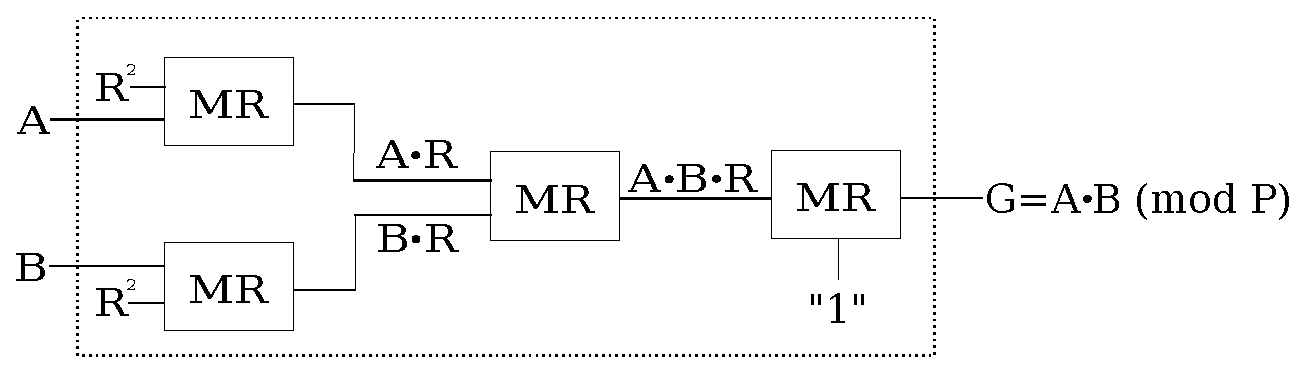
\includegraphics[scale=0.40]{figures/mmcircuit}
%	\end{center}
%	\caption{Montgomery multiplier over $\mathbb{F}_{2^k}$}
%	\label{fig:mm4}
%\end{figure}
Montgomery multipliers are typically designed hierarchically, as shown in Fig. \ref{fig:mm4}. 
If the hierarchy is known, it can be
exploited by computing the abstraction of each MR block in parallel, as shown in 
Table \ref{tbl:montBlkToolResults}.
In this table, 'BLK A' and 'B' denote the input MR blocks, 'BLK
Mid' denotes the middle block and 'BLK Out' is the output block. While
each block is an MR block, some have been simplified by
constant-propagation, hence they have
different sizes. First, a polynomial is extracted for each MR block
(gate-level to word-level abstraction), and then the approach is
re-applied at word-level to derive the input-output relation (solved
trivially in $< 1$ second). Our approach can extract the word-level
polynomial for up to 571-bit circuits! 

%\setlength{\abovecaptionskip}{3pt}
\begin{table}[hbt]
\begin{center}
{\small
\caption{Abstraction of flat Montgomery multipliers. Time given in seconds, memory given in MB. $TO$ = $3$ days ($259,200$ seconds.}
\label{tbl:montFlatToolResults}
%\noindent\resizebox{\textwidth}{!}{%
\begin{tabular}{|l|r|c|c|c|c|c|c|c|} 
\hline
\multicolumn{2}{|c|}{Size (k)}      &  163  &     233 &     283 &     409 & 571 \\
\multicolumn{2}{|c|}{\# of Gates}   & 184K  &    329K &    488K &    1.0M & 1.97M \\
%% \hline
%% \multirow{2}{*}{Singular} & Time    &    -     &    -    &    -    &    -    &    -      \\
%%                           & Max Mem &    -     &    -    &    -    &    -    &    -      \\
\hline
\multirow{2}{*}{Time} & Bug Free &   6,897  &  63,805 &  TO & TO  &   TO \\
                      & Buggy    &   6,961  &  64,009 &  TO & TO  &   TO      \\
\hline
\multicolumn{2}{|c|}{Max Memory} &     153  &     325 &     505 &    971  &   2,240   \\
\hline
\end{tabular}
%}
}
\end{center}
\vspace{-0.15in}
\end{table}

\begin{table}[hbt]
\begin{center}
{\small
\caption{Abstraction of Montgomery blocks. Time given in seconds, memory is given in MB. TO = 3 days (259,200 seconds)}
\label{tbl:montBlkToolResults}
%\noindent\resizebox{\textwidth}{!}{%
\begin{tabular}{|l|r|c|c|c|c|c|c|} 
\hline
\multicolumn{3}{|c|}{Circuit Size (k)}                          &    163 &      233 &     283 &     409 &     571 \\
\hline
\multicolumn{2}{|c|}{\multirow{4}{*}{\# of Gates}}    & Blk A   & 33K &   55K &  82K & 168K & 330K \\
\multicolumn{2}{|c|}{}                                & Blk B   & 33K &   55K &  82K & 168K & 330K \\
\multicolumn{2}{|c|}{}                                & Blk Mid & 85K &  163K & 241K & 502K & 980K \\
\multicolumn{2}{|c|}{}                                & Blk Out & 32K &   54K &  81K & 168K & 328K \\
\hline
%% \multirow{6}{*}{Singular}    & \multirow{4}{*}{Time}  & Blk A   & 22,860  &    -    &    -    &    -    &    -    \\
%%                              &                        & Blk B   & 19,476  &    -    &    -    &    -    &    -    \\
%%                              &                        & Blk Mid & 18,010  &    -    &    -    &    -    &    -    \\
%%                              &                        & Blk Out & 17,604  &    -    &    -    &    -    &    -    \\
%% \hhline{~-----------}
%%                              & \multicolumn{2}{|r|}{Total Time} & 77,950  &    -    &    -    &    -    &    -    \\
%%                              & \multicolumn{2}{|r|}{Max Mem}    & 58,266  &    -    &    -    &    -    &    -    \\
%% \hline
%                                                             163       233       283      409       571
\multirow{8}{*}{Time} &\multirow{4}{*}{Bug Free}& Blk A   &    25 &      142 &     330 &   1,322 &   5,371 \\
                      &                         & Blk B   &    25 &      141 &     329 &   1,335 &   5,241 \\
                      &                         & Blk Mid &    73 &      408 &     883 &   4,471 &  19,942 \\
                      &                         & Blk Out &    24 &      140 &     321 &   1,338 &   5,532 \\
\hhline{~-------}
                      &\multirow{4}{*}{Buggy}   & Blk A   &    26 &      142 &     331 &   1,323 &   5,372 \\
                      &                         & Blk B   &    26 &      141 &     330 &   1,336 &   5,421 \\
                      &                         & Blk Mid &   111 &      580 &   1,411 &   6,829 &  37,804 \\
                      &                         & Blk Out &    25 &      141 &     322 &   1,339 &   5,539 \\
\hline%{~-----------}
%\multicolumn{3}{|r|}{Total Time}                          &    636 &    1,909 &   8,186 &  34,002 &  87,458 \\
\multicolumn{3}{|r|}{Max Mem Per Blk}                      &    80 &      168 &    254 &     538 &   1,129 \\
\hline

\end{tabular}
%}
}
\end{center}
\vspace{-0.2in}
\end{table}

%A multiplier over $\Fkk$ can also be composed over the composite field
%$\Fm_{(2^m)^n}$, where $k = m\cdot n$. The input $A=a_0+a_1\alpha+\dots+a_{k-1}\alpha^{k-1}$ is 
%transformed into multiple word-level input blocks over $\Fm_{2^m}$, $A_0,A_1,\dots,A_{n-1}$,
%where each $A_i=a_{i0}+a_{i1}\beta+\dots+a_{i(m-1)}\beta^{m-1}$ 
%and $\beta$ is the primitive element of $\Fm_{2^m}$. The multiplier is then 
%composed of m-bit blocks, each of which is either an m-bit adder or an m-bit 
%multiplier over $\Fm_{2^m}$. 
%An example $4$-bit multiplier with designed over $\Fm_{(2^2)^2}$ is 
%seen in Figure \ref{fig:comp4ex}. 
To abstract a word-level representation of the 
composite field multiplier $\F_{(2^m)^n}$ [Fig. \ref{fig:comp4ex}], we
first apply our approach to abstract a word-level representation of each m-bit block. 
In the case of an adder, this abstraction is trivially computed in $1$ second. 
In the case of a multiplier, 
refer to our experimental results for Mastrovito multipliers for comparison (Table \ref{tbl:mastroToolresults})
as these are designed as $m$-bit Mastrovito blocks. Each abstraction can be computed independently. 
Once these word-level abstractions are known, the final abstraction over $\F_{(2^m)^n}$ is performed
using only word-level variables. 
%For this, a functional mapping from each 
%$A_i$ to $A$ is needed in the form $A_i=\F_i(A)$. This is computed in a similarly 
%to the bit-level functional mapping $a_i=\F_i(A)$ described in 
%Section \ref{sec:improve}, except here the property $A_i^{2^m}=A_i$ is exploited 
%instead of the property $a_i^2=a_i$.
The results of this final word-level abstraction of 
buggy and bug-free multipliers over composite fields are shown in 
Table \ref{tbl:compositeToolResults}.

%\centering
%\begin{subfigure}{.4\columnwidth}
%\includegraphics[width=\columnwidth]{example-image-a}%
%\caption{cap a}%
%\label{subfiga}%
%\end{subfigure}\hfill%
%\begin{subfigure}{.4\columnwidth}
%\includegraphics[width=\columnwidth]{example-image-b}%
%\caption{cap b}%
%\label{subfigb}%
%\end{subfigure}\hfill%
%\begin{subfigure}{.4\columnwidth}
%\includegraphics[width=\columnwidth]{example-image-c}%
%\caption{cap c}%
%\label{subfigc}%
%\end{subfigure}%
%\caption{The proper caption}
%\label{figabc}
%\end{figure*}



%\begin{figure*}[t]
%        \centering
%        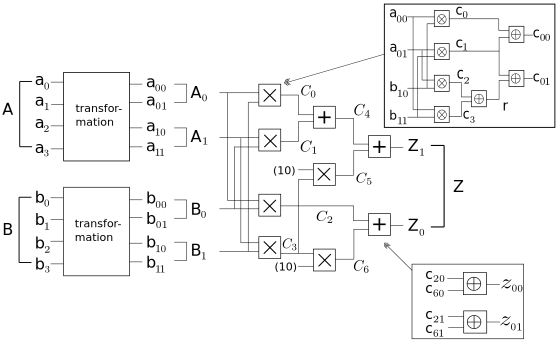
\includegraphics[width=.75\linewidth]{./figures/compMineSmall}
%        \caption{$4$-bit composite multiplier designed over $\Fm_{(2^2)^2}$}\label{fig:comp4ex}
%\end{figure*}

\begin{table}[!h]
\centering
{
\small
%\begin{tabular}{||c|c|c|c|c|c||c|c|c|c|c|c||c|c|c|c|c|c||} 
%\hline
%\multicolumn{6}{||c||}{64}&\multicolumn{6}{c||}{128}&\multicolumn{6}{c||}{256}\\
%\hline
%\multirow{2}{*}{$m$} &  \multirow{2}{*}{$n$} & \multicolumn{2}{c|}{Bug Free} & \multicolumn{2}{c||}{Buggy} &
%\multirow{2}{*}{$m$} &  \multirow{2}{*}{$n$} & \multicolumn{2}{c|}{Bug Free} & \multicolumn{2}{c||}{Buggy} &
%\multirow{2}{*}{$m$} &  \multirow{2}{*}{$n$} & \multicolumn{2}{c|}{Bug Free} & \multicolumn{2}{c||}{Buggy}   \\
%\hhline{~~----~~----~~----}
%     &       & Time    &   Mem   & Time     &   Mem &
%     &       & Time    &   Mem   & Time     &   Mem &
%     &       & Time    &   Mem   & Time     &   Mem\\
%\hline
%$2$  & $32$  & $4$     &  $4$    & $4$      & $10$  &
%$2$  & $64$  & $188$   & $11$    & $118$    & $32$  &
%$2$  & $128$ & $10,602$& $45$    & $10,617$ & $126$ \\
%\hline
%$4$  & $16$  & $7$     &   $5$   & $7$      & $11$  &
%$4$  & $32$  & $271$   &   $15$  &  $272$   & $36$  &
%$4$  & $64$  & $23,876$&   $61$  & $23,910$ & $142$ \\
%\hline
%$8$  & $8$  &  $9$     &  $5$    & $9$      & $11$  &
%$8$  & $16$ & $412$    &  $17$   &  $414$   & $38$ &
%$8$  & $32$ & $32,247$ &  $69$   & $32,293$ & $150$ \\
%\hline
%$16$ & $4$  & $11$     &  $5$    & $11$     & $11$  &
%$16$ & $8$  & $513$    & $19$    & $514$    & $40$ &
%$16$ & $16$ & $41,594$ & $74$    & $41,651$ & $155$ \\
%\hline
%$32$ & $2$  & $12$     &  $5$    & $12$     & $12$  &
%$32$ & $4$  & $545$    & $19$    & $546$    & $40$ &
%$32$ &  $8$ & $46,223$ & $75$    & $46,285$ & $156$ \\
%\hline
%   - &   -  &   -      &      -  &        - &      - &
%$64$ & $2$  & $563$    & $19$    &  $565$   & $40$&
%$64$ &  $4$ & $49,466$ & $75$    & $49,532$ &  $156$ \\
%\hline
%  -   &   - &   -      &    -    &    -     &     -  &
%  -   &   - &   -      &    -    &    -     &     -  &
%$128$ & $2$ & $55,440$ & $76$    & $55,513$ &  $157$ \\
%\hline
%\end{tabular}
%\begin{tabular}{|c|c|c|c|c|}
%\hline
%\multicolumn{5}{|c|}{64}\\
%\hline
%\multirow{2}{*}{$m$} &  \multirow{2}{*}{$n$} & \multicolumn{2}{c|}{Time} & Max \\
%\hhline{~~--~}
%     &       & Bug Free    &   Buggy   &   Mem \\
%\hline
%$2$  & $32$  & $4$     & $4$      & $10$  \\
%\hline
%$4$  & $16$  & $7$     & $7$      & $11$  \\
%\hline
%$8$  & $8$  &  $9$     & $9$      & $11$  \\
%\hline
%$16$ & $4$  & $11$     & $11$     & $11$  \\
%\hline
%$32$ & $2$  & $12$     & $12$     & $12$  \\
%\hline
%   - &   -  &   -      &        - &      -\\
%\hline
%  -   &   - &   -      &    -     &     - \\
%\hline
%\end{tabular}

\begin{tabular}{|c|c|c|c|c|}
\hline
\multicolumn{5}{|c|}{128}\\
\hline
\multirow{2}{*}{$m$} &  \multirow{2}{*}{$n$} & \multicolumn{2}{c|}{Time} & Max \\
\hhline{~~--~}
     &      & Bug Free & Buggy & Mem \\
\hline
 $2$ & $64$ &      $1$ &   $1$ & $4$ \\
\hline
 $4$ & $32$ &      $1$ &   $1$ & $2$ \\
\hline
 $8$ & $16$ &      $1$ &   $1$ & $2$ \\
\hline
$16$ &  $8$ &      $1$ &   $1$ & $2$ \\
\hline
$32$ &  $4$ &      $1$ &   $1$ & $2$ \\
\hline
$64$ &  $2$ &      $1$ &   $1$ & $3$ \\
\hline
  -  &   -  &   -      &   -   &  -  \\
\hline
  -  &   -  &   -      &   -   &  -  \\
\hline
  -  &   -  &   -      &   -   &  -  \\
\hline
\end{tabular}
\begin{tabular}{|c|c|c|c|c|}
\hline
\multicolumn{5}{|c|}{256}\\
\hline
\multirow{2}{*}{$m$} &  \multirow{2}{*}{$n$} & \multicolumn{2}{c|}{Time} & Max \\
\hhline{~~--~}
     &        & Bug Free & Buggy & Mem  \\
\hline
  $2$ & $128$ &     $15$ &  $15$ & $23$ \\
\hline
  $4$ &  $64$ &      $2$ &   $2$ &  $4$ \\
\hline
  $8$ &  $32$ &      $1$ &   $1$ &  $3$ \\
\hline
 $16$ &  $16$ &      $1$ &   $1$ &  $2$ \\
\hline
 $32$ &   $8$ &      $1$ &   $1$ &  $2$ \\
\hline
 $64$ &   $4$ &      $1$ &   $1$ &  $2$ \\
\hline
$128$ &   $2$ &      $1$ &   $1$ &  $2$ \\
\hline
  -   &   -   &       -  &    -  &   -  \\
\hline
  -   &   -   &       -  &    -  &   -  \\
\hline
\end{tabular}
\begin{tabular}{|c|c|c|c|c|}
\hline
\multicolumn{5}{|c|}{512}\\
\hline
\multirow{2}{*}{$m$} &  \multirow{2}{*}{$n$} & \multicolumn{2}{c|}{Time} & Max \\
\hhline{~~--~}
     &        & Bug Free & Buggy & Mem  \\
\hline
  $2$ & $256$ &    $406$ & $408$ & $90$ \\
\hline
  $4$ & $128$ &     $53$ &  $53$ & $25$ \\
\hline
  $8$ &  $64$ &      $8$ &   $8$ &  $4$ \\
\hline
 $16$ &  $32$ &      $2$ &   $2$ &  $4$ \\
\hline
 $32$ &  $16$ &      $1$ &   $1$ &  $3$ \\
\hline
 $64$ &   $8$ &      $1$ &   $1$ &  $3$ \\
\hline
$128$ &   $4$ &      $1$ &   $1$ &  $2$ \\
\hline
$256$ &   $2$ &      $1$ &   $1$ &  $2$ \\
\hline
  -   &   -   &      -   &   -   &   -  \\
\hline
\end{tabular}
\begin{tabular}{|c|c|c|c|c|}
\hline
\multicolumn{5}{|c|}{1024}\\
\hline
\multirow{2}{*}{$m$} &  \multirow{2}{*}{$n$} & \multicolumn{2}{c|}{Time} & Max \\
\hhline{~~--~}
      &       & Bug Free &  Buggy   &   Mem \\
\hline
  $2$ & $512$ & $11,883$ & $12,050$ & $414$ \\
\hline
  $4$ & $256$ &  $1,520$ &  $1,536$ & $106$ \\
\hline
  $8$ & $128$ &    $209$ &    $211$ &  $29$ \\
\hline
 $16$ &  $64$ &     $38$ &     $37$ &  $10$ \\
\hline
 $32$ &  $32$ &     $10$ &     $10$ &   $5$ \\
\hline
 $64$ &  $16$ &      $4$ &      $4$ &   $3$ \\
\hline
$128$ &   $8$ &      $2$ &      $2$ &   $3$ \\
\hline
$256$ &   $4$ &      $1$ &      $1$ &   $3$ \\
\hline
$512$ &   $2$ &      $1$ &      $1$ &   $3$ \\
\hline
\end{tabular}
}
\caption{Abstraction of bug-free Mastrovito multipliers over $\mathbb{F}_{(2^m)^n}$. Time is given in seconds. Memory is given in MB. $TO$ = more than $24$ hours = $86,400$ seconds. 
Note that abstractions of the $m$-bit blocks which compose the circuits are already known.}
\label{tbl:compositeToolResults}
\end{table}


\begin{table}[!hbt]
\begin{center}
{\small
\caption{Statistics of Designs over $\mathbb{F}_{(2^m)^n}$}
\label{tbl:stats}
\begin{tabular}{|c|c|c|c|c|c|c|c|} 
\hline
$n$ & 2 & 4 & 8 & 16 & 32 \\
\hline
\# of $\F_{2^m}$ Multipliers  & $6$ & $36$ & $168$ & $720$ & $2976$ \\
\hline
\# of $\F_{2^m}$ Adders       & $3$ & $27$ & $147$ & $675$ & $2883$  \\
\hline
\end{tabular}
}
\end{center}
\end{table}


%% For these
%% experiments, we used the Singular \cite{DGPS} computer algebra
%% tool. The results are shown in Table \ref{tab:ours}. The row
%% ``Compute-GB'' depicts the time required to compute the Gr\"obner
%% basis using the abstraction term order; whereas the row ``Improved-GB''
%% depicts the result of our improved, guided, approach using RATO. We
%% correctly identified $Z + A\cdot B$ as the only word-level polynomial
%% in the Gr\"obner basis $G'$, for up to 163-bit circuits over
%% ${\mathbb{F}}_{2^{163}}$. Similarly, the results for Montgomery
%% multipliers are shown in Table \ref{tab:mont}. Montgomery multipliers
%% are significantly larger than Mastrovito ones. The 163-bit circuit has
%% more than $91,000$ variables, which Singular cannot accommodate, as
%% its capacity is limited to $< 32767$ variables. Therefore, the largest
%% experiment was restricted to 128-bit Montgomery multipliers. 
%% These experiments were conducted  on a desktop with $2.40$GHz Intel
%% Core \texttrademark{$2$} Quad CPU with $8$GB memory running $64$-bit
%% Linux. 


The above experiments also demonstrate that we can perform equivalence
checking between Mastrovito (golden model) and Montgomery multiplier
(implementation) circuits, by deriving a canonical polynomial ($Z_1,
Z_2$)from each circuit independently and then checking if $Z_1 =
Z_2$, for up to 571-bit circuits. Our experiments have shown that contemporary 
approaches (BDDs, SAT, SMT, and AIG/ABC) show some success in bug-catching for these
kinds of circuits (particularly ABC). These experiments are shown in Table \ref{tab:satsmtbugcatch}.
Note that ABC uses random simulation for FRAIGing (functionally reducing AIGs), which
can catch a bug early if it is lucky.
However, full equivalence checking using any of these techniques failed even for 
16-bit circuits, as shown in Table \ref{tab:equivCheckFail}.

\begin{table}[!hbt]
\begin{center}
{\small
\caption{Bug-catching between a golden-model Mastrovito and buggy Montgomery circuit. 
Time given in seconds. TO = 3 days (259,200 seconds)}
\label{tab:satsmtbugcatch}
%\noindent\resizebox{\textwidth}{!}{%
\begin{tabular}{|l|c|c|c|c|c|c|} 
\hline
Circuit Size (k) &  64  &    163 &      233 &     283 &     409 &    571  \\
\hline
ABC              &  1     &    32  &     6    &   96    &     217 &    401  \\
\hline
Lingeling        &  1     &     8  &    362   & 12,728  &   3,323 & 23,298  \\
\hline
Picosat          & 15,235 &    TO  &    TO    &    TO   &     TO  &   TO    \\
\hline
Boolector        &  4     &    30  &    41    &   105   &    152  & 19,113  \\
\hline
CVC4             &  2     &    11  &    64    &  8,660  &    280  &    TO   \\
\hline
Z3               &  1     &    12  &    55    & 10,169  &    335  &    TO   \\
\hline
Yices            &  1     &     6  &     7    &   618   &    578  & 11,568  \\
\hline
\end{tabular}
%}
}
\end{center}
\vspace{-0.2in}
\end{table}

\begin{table}[!hbt]
\begin{center}
{\small
\caption{Equivalence checking between a golden-model Mastrovito and a bug-free Montgomery circuit. 
TO = 3 days (259,200 seconds)}
\label{tab:equivCheckFail}
%\noindent\resizebox{\textwidth}{!}
}
\end{center}
\vspace{-0.2in}
\end{table}

%between f, 
%as shown in Table III, these tools have shown
% In \cite{lv:date2012}, the authors
%have shown that this same equivalence checking experiment using
%contemporary approaches (BDDs, SAT, SMT, and AIG/ABC) is infeasible
%beyond 16-bit circuits (cf. Table I in \cite{lv:date2012}). 

%, the table is not reproduced here due to lack of space).   

%% \begin{table}[hbt!]
%% {\myfontsize
%% \begin{center}
%% \caption{\small Run-time for word-level abstraction from Mastrovito
%%   multipliers using our approach.  {\sc Singular} computer algebra
%%   tool is used for this experiments. Time is given in seconds. MO = out
%%   of memory.}  
%% \label{tab:ours}
%% \begin{tabular}{|l||c|c|c|c|c|c|c|} \hline 
%% Size $k$-bits& 16 & 32  & 64 & 128  &163\\
%% \hline
%% \#variables &$323$ &$1155$ &$4355$ &$16899$ &$27224$ \\
%% \hline
%% \#polynomials &$291$ &$1091$  &$4227$ &$16643$ &$26989$ \\
%% \hline
%% \#terms &$1793$ &$7169$  &$28673$ &$114689$ &$185984$ \\
%% \hline
%% Compute-GB & $124$ &$720$  &$MO$ &$MO$ &$MO$ \\
%% \hline
%% Improved-GB &$0.04$ &$1.6$ &$78$ &$4500$ &$18424$ \\
%% \hline
%% %Our approach: Bugs (s) & $0.04$ &$1.43$  &$114.86$ &$788.65$ &$3061$  &$9384$
%% % &$16368$\\
%% \hline
%% \end{tabular}
%% \end{center}
%% \vspace{-0.2in}
%% }
%% \end{table}



%% \begin{table}[htb!]
%% {\myfontsize
%% \begin{center}
%% \caption{ Runtime for word-level abstraction from Montgomery
%%   multipliers. TO = timeout of 10hrs. Time is given
%%   in seconds. $\ast$ denotes {\sc singular}'s capacity exceeded.} 
%% \label{tab:mont}
%% \begin{tabular}{|c||c|c|c|c|c|c|} \hline 
%% Operand size $k$ &  32 & 48 & 64 & 128 &163\\
%% \hline
%% \#variables     &$1194$     &$2280$     &$4395$     &$14122$  &$91246$\\
%% \hline
%% \#polynomials    &$1130$     &$2184$     &$4267$     &$13866$  &$89917$\\
%% \hline
%% \#terms          &$10741$    &$18199$    &$40021$    &$134887$ &$484738$\\
%% \hline \hline
%% %Compute-GB &$1.50$  &$11.03$    &$27.70$  &$10919$  &$\ast$\\
%% %\hline
%% Improved-GB    &$25$     &$1023$     &$3060$     &$11047$    &$\ast$\\
%% \hline
%% \end{tabular}
%% \end{center}
%% }
%% \end{table}

%\afterpage{\clearpage}
\FloatBarrier

\section{Limitations of the Abstraction Approach}

Our tools and approach performs very favorable for $\Fkk$ multiplier circuits and other 
functions designed over fields. These types of circuits are based on AND-XOR gate logic. 
Thus, the polynomials 
derived during the reduction procedures are very sparse. Since the  
complexity of the algorithm heavily depends on the density of the polynomials,
the worst-case is avoided in such designs.
In the case of bugs within these circuits, these polynomials increase in size, but are
still easily manageable. This is why the approach is applicable to
very large Galois field multipliers, both buggy and bug-free.

However, for random logic, especially logic containing chains of
OR gates, the polynomial becomes very dense. As a result, the algorithm begins 
to encounter the computational worst-case.  
This is best shown with a small example.

\begin{Example}
\begin{figure}[h]
        \centering
        \begin{subfloat}[][XOR logic]{%{0.25\textwidth}
                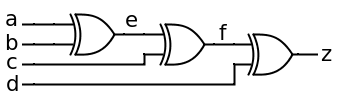
\includegraphics[width=0.25\textwidth]{./figures/xor-example}
                %\caption{XOR logic}
                \label{fig:xorEx}}
        \end{subfloat}%
        ~ %add desired spacing between images, e. g. ~, \quad, \qquad, \hfill etc.
          %(or a blank line to force the subfigure onto a new line)
        \begin{subfloat}[][OR logic]{%{0.25\textwidth}
                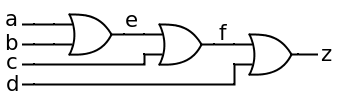
\includegraphics[width=0.25\textwidth]{./figures/or-example}
                %\caption{OR logc}
                \label{fig:orEx}}
        \end{subfloat}
        \caption{Logic comparisons}\label{fig:logicExmp}
\end{figure}


%\begin{figure}[!hbt]
%\centerline{
%\includegraphics[scale=0.5]{}
%}
%\caption{ XOR-based logic.}
%\label{fig:xorEx}
%\end{figure}
{\it 
Consider the circuit in Figure \ref{fig:xorEx}, which performs a 4-input
XOR function. Due to RATO, the monomial ordering of the variables is 
$z > f > e > d > c> b >a$. Thus, $z$ will be reduced in terms of the rest of the 
variables. The polynomials derived from the design are:
\begin{eqnarray}
f_1:z+f+d & f_2:f+e+c & f_3:e+b+a \nonumber
\end{eqnarray}
The reduction procedure $z \xrightarrow{f_1,f_2,f_3}_+ r$ will be computed as follows:
\begin{enumerate}
\item $z \xrightarrow{z+f+d} f+d$
\item $(f+d)\xrightarrow{f+e+c}e+d+c$
\item $(e+d+c)\xrightarrow{e+b+a}d+c+b+a$
\end{enumerate}
In each reduction, the output gate variable is removed and one copy of each 
input variable is added, leaving a sparse polynomial. Now consider the same 
circuit with the XOR gates replaced by OR gates, as shown in Figure \ref{fig:orEx}.

%\end{figure}
%\begin{figure}[!hbt]
%\centerline{
%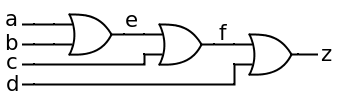
\includegraphics[scale=0.5]{./figures/or-example}
%}
%\caption{ OR-based logic.}
%\label{fig:orEx}
%\end{figure}
The monomial ordering stays the same, but the polynomials derived from each gate
have changed:

\begin{eqnarray}
f_1:z+fd+f+d & f_2:f+ec+e+c & f_3:e+ba+b+a \nonumber
\end{eqnarray}
The reduction procedure, $z \xrightarrow{f_1,f_2,f_3}_+ r$ is now computed as:
\begin{enumerate}
\item $z \xrightarrow{z+fd+f+d}fd+f+d$
\item $(fd+f+d)\xrightarrow{f+ec+e+c}f+edc+ed+dc+d$;\\
$(f+edc+ed+dc+d)\xrightarrow{f+ec+e+c}edc+ed+ec+e+dc+d+c$
\item $(edc+ed+ec+e+dc+d+c)\xrightarrow{e+ba+b+a}_+$\\ $dcba+dcb+dca+dba+dc+db+da+d+cba+cb+ca+c+ba+b+a$
\end{enumerate}
Each pass removes an output variable of the gate, but replaces it with two instances of each input variable.
This increases the density of the resulting polynomial exponentially.
}
\end{Example}

\section{Conclusions}

This chapter examined the data structures and algorithms implemented in a
custom software abstraction tool.
Abstraction of Galois field circuits using the custom tool has 
greatly better performance compared to using {\sc Singular} scripts. With it, we can
abstract circuits up to $1024$-bits, buggy or bug-free. Although a bug will 
generally substantially inflate the size of the resulting polynomial abstraction, 
the tool is not greatly hindered by the presence of bugs in a circuit.
However, for random logic, especially OR-based logic, the size of the polynomials tends 
to grow exponentially during the abstraction. Thus, the approach is infeasible for
circuits with OR-gate chains.

%\include{equiv}
%\chapter{Applications of Word-Level Abstraction of Galois Field 
Circuits}
\label{ch:prop}

In this chapter, we propose two additional applications of word-level 
abstractions
of Galois field circuits. First, we propose an approach to partition
any Galois field arithmetic circuit over $\Fkk$ into sub-circuit  
blocks, each of which can then be analyzed over the same field $\Fkk$.
As each block is a smaller partition of the overall circuit, the 
abstraction complexity of each partition is smaller. Thus, 
word-level abstraction
of the sub-circuits is faster than abstraction of the original circuit.
Abstraction of each sub-circuit can be performed independent of each other,
after which the word-level representations can be combined to find the 
overall function of the entire circuit.
Second, we propose a method for applying our abstraction approach to 
combinational circuits whose function maps one Galois field to 
a different one,
i.e. $f:F_{2^k} \rightarrow F_{2^j}$ where $k \neq j$.

\section{Partitioning Algorithm}
Galois field arithmetic circuits of practical sizes are very large.
As the size of these circuits increase, the computational complexity of a
word-level abstraction increases exponentially.

However, if a large circuit is partitioned, that is 
seperated into smaller seperate pieces, the complexity of each partition is 
smaller and and thus each partition is more manageable.
For word-level abstraction of a circuit, an abstraction of each partition
could be performed and then the word-level representations could be combined
to find the overall word-level representation on the entire circuit.
In addition, each piece
could be abstracted in parallel, thus decreasing the time to
find the overall abstraction.
Recall our abstractions results of the Montgomery multiplier circuits, shown
in Table \ref{tab:absmontflatresults} for a 'flat' abstraction
and Table \ref{tab:absmontresults} for block abstractions. The Montgomery
circuit structure is shown in Figure \ref{fig:montmont}.

\begin{figure}[H]
	\begin{center}
	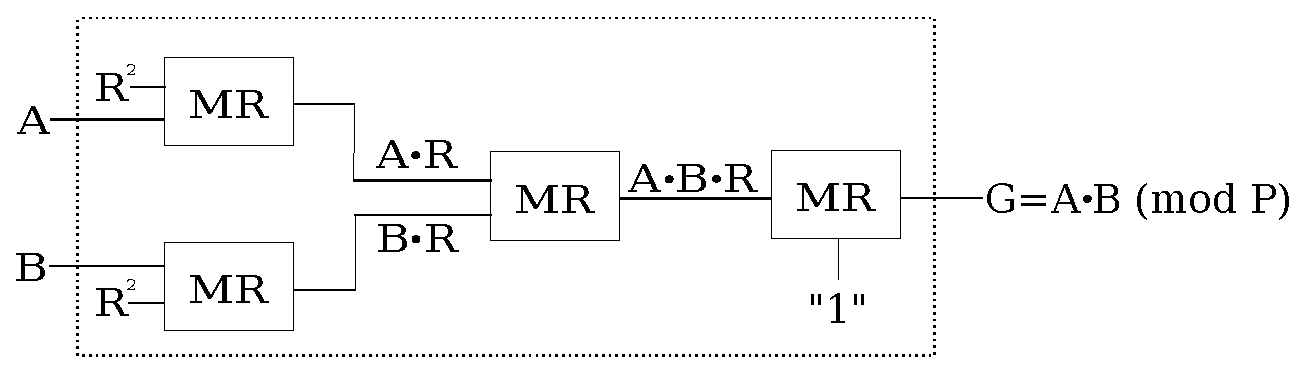
\includegraphics[scale=0.50]{figures/mmcircuit}
	\end{center}
	\caption{Montgomery multiplier over $\mathbb{F}_{2^k}$}
	\label{fig:montblock}
\end{figure}

Each block of the multiplier could be considered a partition. By 
comparing our results for the flat multiplier to the results of each 
block, the power of partitioning becomes apparent. Since the block 
abstractions can be performed in parallel, the time for an 
overall word-level abstraction is based on the time of the slowest block
abstraction.

\subsection{Partition Problem Statement}

The goal of our proposed partitioning algorithm 
is to quickly find partitions for any circuit. 
Given a circuit over $\Fkk$, each partition must have $k$-bit inputs and 
one $k$-bit output for simplicity in calculation.
These restrictions allow us to calculate the polynomial representation of 
each partition over the same field $\Fkk$. Thus, our problem statement is
as follows:

\begin{itemize}
\item Given a Galois field $\Fkk$, i.e. given the corresponding
irreducible polynomial $P(x)$ in $\F[x]$ of degree $k$,
let $P(\alpha) = 0$ where $\alpha \in \Fkk$ is the root of the irreducible
polynomial $P$.
\item  Given a gate-level combinational circuit $C$ with $n$ word-level
$k-bit$ inputs,
$A_1,\dots, A_n \in \Fkk$
and one $k-bit$ output $Z \in \Fkk$.
\item The bit-level primary inputs of the circuit are denoted
$\{a_{0}^{i},a_{1}^{i},\dots,a_{k-1}^{i}\}$, for $i=1,\dots, n$;
the primary bit-level outputs are $\{z_0, \dots, z_{k-1}\} = Z$. 
Note that all $a_{i}^{j}, z_i \in \F_2$.
\item Split the circuit into any number of partitions, $\{P_1,\dots,P_d\}$.
\item Each partition $P$ can have any number of $k-bit$ word-level inputs and
one $k$-bit word-level output.
\item The circuit $C$ must be fully represented by the partitions 
$\{P_1,\dots,P_d\}$.
\end{itemize}

After we have the partitions, $\{P_1,\dots,P_d\}$, if we can abstract a 
word-level polynomial of each partition, we can find the overall word-level 
polynomial function of the circuit $C$ using substitution.

\subsection{Partitioning Approach}

{\it Topological location} from Definition \ref{def:topord} which 
is the maximum number of Boolean logic gates that any path from any input 
must pass to reach a certain node.

\begin{Definition}
The {\bf topological depth} of a combinational circuit is maximum 
topological location of the bit-level outputs of the circuit.
\end{Definition}

First, we find the topological depth $D$ of the circuit $C$. 
Then, we split the circuit approximately in half by finding all nodes $M$ of
depth $\frac{D}{2}$. Ultimately, $M$ must contain exactly
one node in every path from any input to any output of the circuit. 
Thus, for every path which does not contain a node in $M$, 
select a node with the next smallest depth and add it to $M$.
These nodes split the circuit approximately in half. One 
half of the circuit treats $M$ as the bit-level outputs and the other treats 
them as the inputs.

\begin{Example}
Consider the 4-bit Mastrovito multiplier circuit shown
previously in Figure \ref{fig:mas4}. We find the maximum topological depth
of this circuit to be $5$. Thus, we find all nodes with topological
depth $2$ and add them to our nodelist $M$. For every path that does not
contain a node with depth $2$, we add the node with depth $1$ from the path
to $M$.

The topological depth of each node of this circuit is shown in 
Figure \ref{fig:nodes}. Every node in $M$ is highlighted. Note that there
is exactly one node in $M$ for every path through the circuit.

\begin{figure}
	\begin{center}
	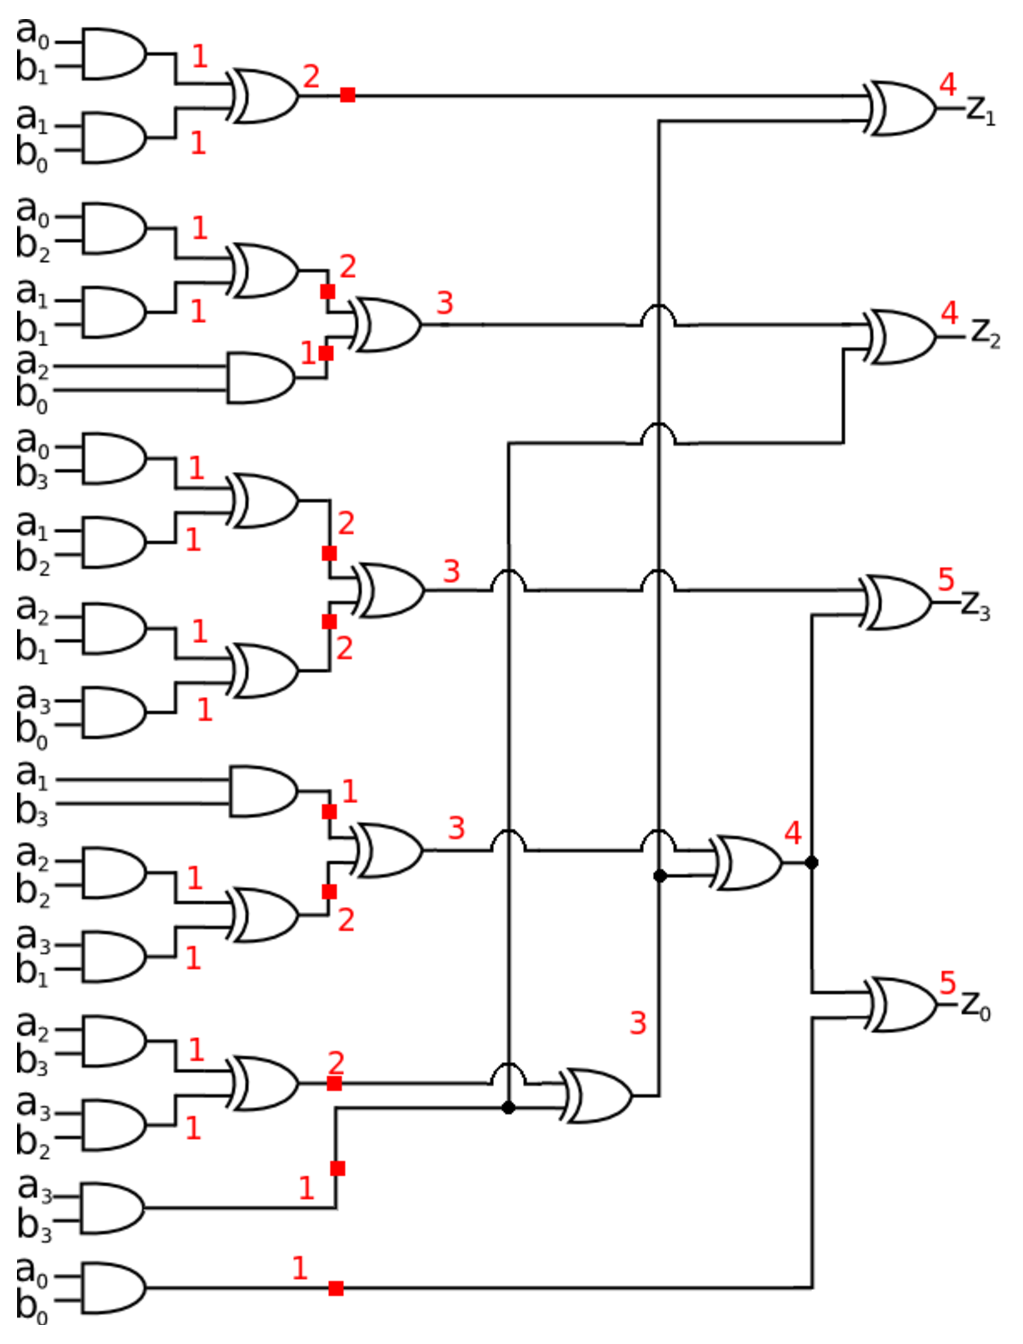
\includegraphics[scale=0.7]{figures/mul4bitTopo2.eps}
	\end{center}
	\caption{Topological Depth and Node Selection}
	\label{fig:nodes}
\end{figure}
\label{exp:mul4topex}
\end{Example}

Now, we the half of the circuit where the nodes $M$ act as the
bit-level outputs.
Select exactly $k$ nodes in $M$, where $k$ is the size of the field $\Fkk$; 
we call these nodes $M_1$. $M_1$ can be considered a $k$-bit word-level 
output. By including every path from $M_1$ to the primary inputs, we 
create a partition $P_1$. Thus, the $k$-bit word-level output of $P_1$ 
are the nodes $M_1$. The $k-bit$ word-level inputs to $P_1$ are the same 
inputs as to the circuit $C$. Thus, $P_1$ is a partition which can be 
analyzed over $\Fkk$.

With $P_1$ designated, select the next $k$ nodes $M_2\subset M$, where $M_2$
contains none of the same nodes as $M_1$. 
Create another partition, $P_2$, where $M_2$ is the $k-bit$ output of $P_2$.
Continue to do this 
until all nodes $M$ have been used in at least one partition.
For the last partition, it is likely that there will be fewer
than $k$ of nodes remaining in $M$ which have not yet been used as the 
output of some partition. 
At this point, select all of the remaining nodes in $M$ which have not been
used
and add in extra nodes in $M$ that have been previously used in a 
partition in order to bring the total to number $k$. Use this collection
of nodes to create the last partition.
Thus, we allow some nodes in $M$ may be outputs of more than one partition, 
although we try to minimize this.
We now have designated $i$ partitions, $P_1 \cdots P_i$, each with a $k$ 
bit output.

\begin{Example}
Refer to the same 4-bit Mastrovito multiplier circuit from Example 
\ref{exp:mul4topex}. We have already found every node $M$. Since $k=4$,
we need to seperate these nodes into groups of $4$ and create partitions
that span from the nodes $M$ to the bit-level inputs 
$\{a_0,\dots,a_3,b_0,\dots,b_3\}$. As there are $10$ nodes in $M$, this will
create $3$ partitions with some nodes in $M$ being
used as the output of more than one partition.

By incrementally selecting $4$ nodes at a time starting at the top, and
labelling the $4$-bit word-level outputs as $H,G,F$, we create partitions
as shown in Figures \ref{fig:part1}, \ref{fig:part2}, and \ref{fig:part3}.

\begin{figure}[H]
	\begin{center}
	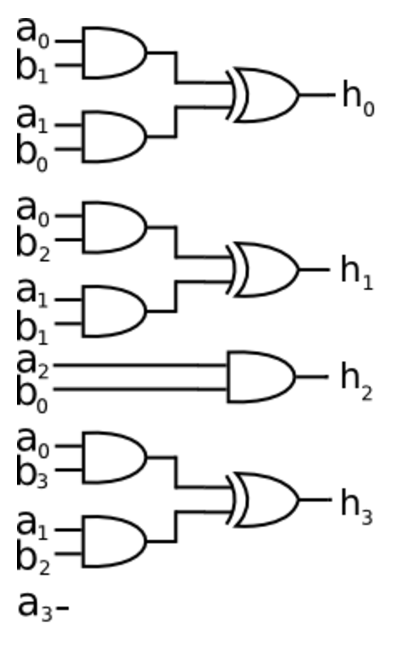
\includegraphics[scale=0.8]{figures/part1.eps}
	\end{center}
	\caption{First Partition, output $H$}
	\label{fig:part1}
\end{figure}

\begin{figure}[H]
	\begin{center}
	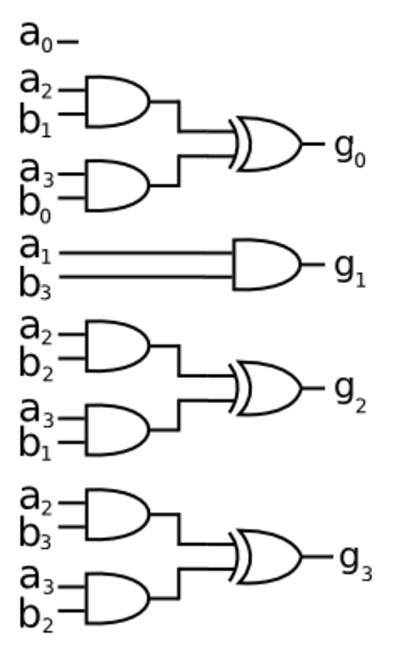
\includegraphics[scale=0.8]{figures/part2.eps}
	\end{center}
	\caption{Second Partition, output $G$}
	\label{fig:part2}
\end{figure}

\begin{figure}[H]
	\begin{center}
	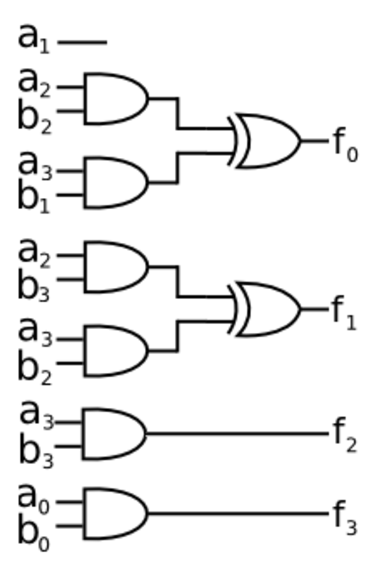
\includegraphics[scale=0.8]{figures/part3.eps}
	\end{center}
	\caption{Third Partition, output $F$}
	\label{fig:part3}
\end{figure}

Note that $f_0=g_2$ and $f_1=g_3$.
\label{exp:mul4inputparts}
\end{Example}

With one half of the circuit partitioned, we look at the other half 
where the nodes in $M$ act as the bit-level inputs. 
The partitions $P_1, \cdots, P_i$ now act as $k$ bit inputs into the second 
half of the circuit. Since there is only one $k$ bit output in the circuit, 
$Z$, we can take the whole second half of the circuit and create one 
partition with $i$ $k$-bit inputs from the outputs of $P_1...P_i$, and one 
$k$ bit output, $Z$. Thus we have partitioned the entire circuit. Since each
partition contains one $k$-bit word-level output and only $k$-bit word-level
inputs, each partition can be analyzed over the same Galois field $\Fkk$ as
the original circuit.

\begin{Example}
Continue the partitioning approach to the 4-bit multiplier
in Example \ref{exp:mul4inputparts}. By using the outputs of the $3$ 
partitions we already have, $\{h_0,\dots,h_1,g_0,\dots,g_3,f_0,\dots,f_3\}$, 
as inputs, we can create the last partition as shown in 
Figure \ref{fig:part4}.

\begin{figure}[H]
	\begin{center}
	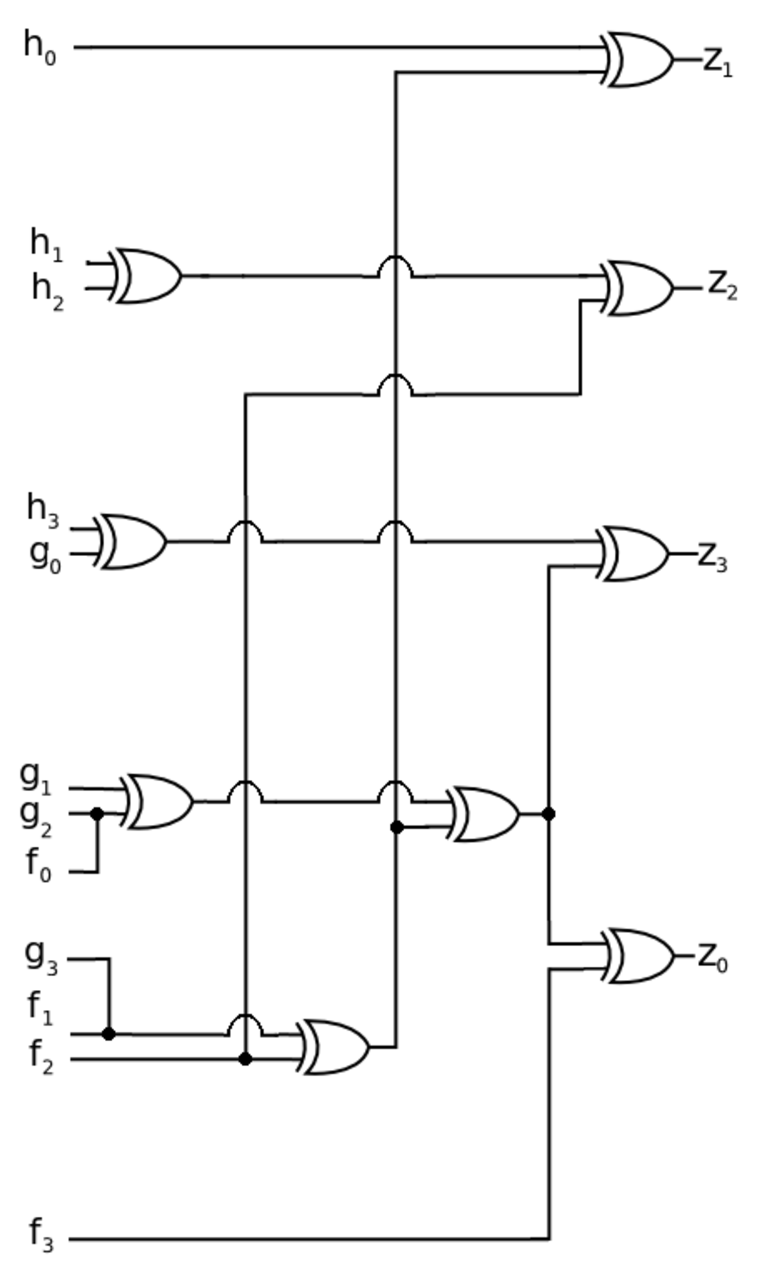
\includegraphics[scale=0.7]{figures/part4.eps}
	\end{center}
	\caption{Fourth Partition}
	\label{fig:part4}
\end{figure}

Thus, the $4$-bit Mastrovito multiplier is fully represented by the four
partitions, as shown in Figure \ref{fig:partitions}.

\begin{figure}[H]
	\begin{center}
	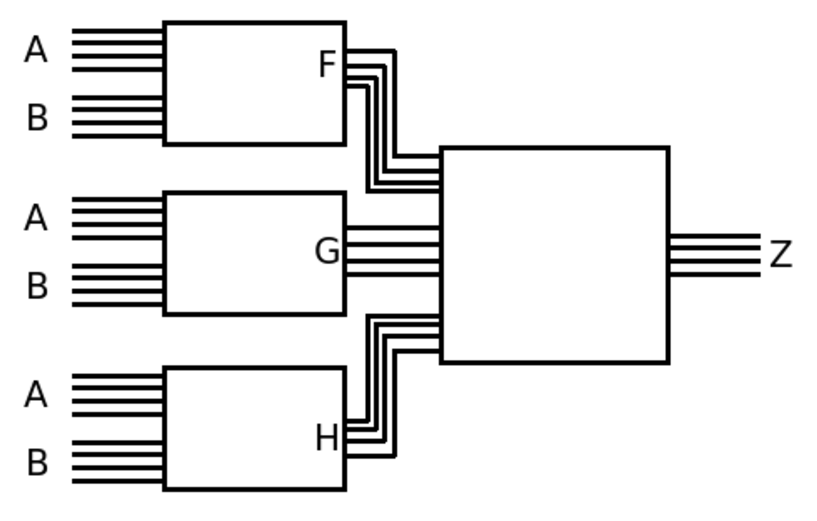
\includegraphics[scale=0.7]{figures/partitions.eps}
	\end{center}
	\caption{Partitioned Circuit Structure}
	\label{fig:partitions}
\end{figure}
\label{exp:mul4partlast}
\end{Example}

\subsection{Overall Approach}
Algorithm \ref{alg:part} is our overall algorithm for creating partitions of 
Galois field arithmetic circuit over $\Fkk$. 

\begin{algorithm}[H]
\SetAlgoNoLine
 \KwIn{$C = $ circuit over $\Fkk$ with $k$ bit input $A$ and $k$ bit output $Z$}
 \KwOut{$P =$ list of circuit partitions}
  $M = $\xspace\{\}\;
  $P = $\xspace\{\}\;
  $D = $ max topological depth of $C$\;
  \For{ every path $T$ in $C$ }
  {
    \For{ every node $N$ in $T$ in reverse topological order }
    {
      \If{ $N \in M$ }
      {
        break\;
      }
      \If{ $N$.depth $<= \frac{D}{2}$ }
      {
        $M = M \cup N$\;
        break\;
      }
    }
  }
  \For{ every $k$ nodes in $M$ as $m_i$ }
  {
  	$P = P$ \xspace$\cup$ partition from $A$ to $m_i$
  }
  $P = P$ \xspace$\cup$ partition from $M$ to $Z$
\caption {General Partitioning Algorithm}\label{alg:part}
\end{algorithm}

Note that while our algorithm proposes to cut the circuit approximately in 
half by finding all nodes of depth $\frac{D}{2}$, this is merely for 
simplicity's sake. This cut can be shifted by changing the depth at which
to search for these nodes. By changing this depth we change the 
relative sizes of the input and output partitions.

\subsection{Applying Abstraction to Circuit Partitions}

Applying abstraction to partitions is similar to applying abstraction to
Montgomery multiplier blocks. We abstract a word-level polynomial 
representation of each partition in parallel. The polynomial abstraction
of the output partition is
\begin{equation}
f_Z: Z + \Func(G_1,\dots,G_i) \nonumber
\end{equation}
where $Z$ is the word-level output of the entire circuit and 
$\{G_1,\dots,G_i\}$ are the word-level outputs of the input partitions
$\{P_1,\dots,P_i\}$. The word-level abstractions of the input partitions are
\begin{eqnarray}
f_1: G_1 + \Func(A_1,\dots,A_n) \nonumber \\
\vdots \\
f_i: G_i + \Func(A_1,\dots,A_n) \nonumber
\end{eqnarray}
where $\{A_1,\dots,A_n\}$.
We are looking for a polynomial in the form of $Z+\Func(A_1,\dots,A_n)$.
Thus, using lex abstraction order $G_1>\dots>G_i>Z>A_1>\dots>A_n$, if we 
perform the reduction $f_Z\stackrel{f_1,\dots,f_i}{\longrightarrow}_+ r$,
$r$ will contain the word-level polynomial $Z+\Func(A_1,\dots,A_n)$.

There are a few issues, however. Every function over $\Fkk$ is a polynomial
function, but for arbitrary logic these polynomial functions can be quite
large. For instance, in $4$-bit multiplier in Example \ref{exp:mul4partlast},
the polynomial word-level abstraction of the partition with output $F$, 
in the form of $F+\Func(A,B)$, is

\begin{eqnarray}
F+(\alpha^3+1)A^8 B^8+(\alpha^2+\alpha)A^8 B^4+A^8 B^2+(\alpha^3+\alpha+1) A^8 B+(\alpha^3+\alpha+1) A^4 B^8 \nonumber \\
+(\alpha+1) A^4 B^4+(\alpha^2+\alpha) A^4 B^2+A^4 B+(\alpha^3+\alpha+1) A^2 B^8+(\alpha^3) A^2 B^2+(\alpha^3+\alpha^2) A B^8 \nonumber \\
+(\alpha^3+\alpha) A B^4+(\alpha^3+\alpha^2) A B^2+(\alpha^3+\alpha+1) A B \nonumber 
\end{eqnarray}

Thus, as the circuit grows in the size, the polynomial abstraction of each
partition will become quite large. This could make reduction time-consuming.
Also, since every partition is random logic over $\Fkk$, our 
abstraction approach that obviates the complexity of \Grobner basis 
computation will always produce a representation that includes bit-
level input variables. Thus, the simple reduction approach shown above will
not work. Thus, in order to seriously consider abstraction with 
partitioning for circuits of applicable sizes, we need to an abstraction 
solution that obviates \Grobner basis complexity and always computes a word-
level representation only.

\section{Analyzing Circuits Over Two Different Galois Fields}

Thus far, our abstraction technique only worked for circuits that perform
a function $\Func$ over $\Fkk$. That is, a circuit which mapped inputs
over $\Fkk$ to outputs over $\Fkk$, $\Func:\Fkk\rightarrow \Fkk$. This
limits the approach only to circuits with inputs and outputs of equal size 
$k$.

In this section, we present a method for abstracting a representation of a
circuit which maps inputs over a field $\F_{2^k}$ to outputs over another
field $F_{2^j}$, where $k \neq j$. 

\subsection{Problem Statement}
A circuit which performs a functional mapping from $\F_{2^k}$ to $\F_{2^n}$
must have $k$-bit word-level inputs and a $j$-bit word-level output. 
Thus, our problem statement is as follows:

\begin{itemize}
\item Given a Galois field $\F_{2^k}$, i.e. given the corresponding
irreducible polynomial $P_k(x)$ in $\F[x]$ of degree $k$,
let $P_k(\beta) = 0$ where $\beta \in \F_{2^k}$ is the root of the 
irreducible polynomial $P_k$.
\item Given another Galois field $\F_{2^j}$, where $j\neq k$, i.e. 
given the corresponding
irreducible polynomial $P_j(x)$ in $\F[x]$ of degree $j$,
let $P_j(\gamma) = 0$ where $\gamma \in \F_{2^j}$ is the root of the 
irreducible polynomial $P_j$.
\item Given another Galois field $\F_{2^h}$, where $h=lcm(j,k)$, i.e. 
given the corresponding
irreducible polynomial $P_h(x)$ in $\F[x]$ of degree $h$,
let $P_h(\alpha) = 0$ where $\alpha \in \F_{2^h}$ is the root of the 
irreducible polynomial $P_h$.
\item Given a gate-level combinational circuit $C$ with
word-level $k$-bit input $A \in \Fkk$, and
and $j$-bit output $Z \in \F_{2^j}$.
\item The bit-level primary input of the circuit is denoted
$\{a_0,\dots,a_{k-1}\} \in \F_2$,
the primary bit-level outputs are $\{z_0, \dots, z_{j-1}\} \in \F_2$.
\item The word-level primary input is denoted 
$A = a_0 + a_1\beta + \dots + a_{k-1}\beta^{k-1}$ and the word-level 
primary output is denoted $Z = z_0 + z_1\gamma + \dots + z_{j-1}\gamma^{j-1}$
\item Find the word-level polynomial function $\Func$ over $\F_{2^h}$
performed by $C$ in the form of $Z=\Func(A_1, \dots, A_n)$.
\end{itemize}

Since the word-level inputs $\{A_1, \dots, A_n\} \in \Fkk$ and the
word-level output $Z \in \F_{2^j}$, the abstraction polynomial 
$Z+\Func(A_1, \dots, A_n)$ must be in $\F_{2^h}$ where 
$\Fkk \subset \F_{2^h}$ and $\F_{2^j} \subset \F_{2^h}$. In other words,
the word-level polynomial is contained in the smallest field that contains 
both the input field $\Fkk$ and output field $\F_{2^j}$. Thus, $h=lcm(k,j)$.

\subsection{Problem Formulation}

Since the abstraction polynomial representation is over the field 
$\F_{2^h}$, we need to model the entire circuit as a system of polynomials 
over this field (as shown in our abstraction chapter).
The only polynomials that cannot be 
immediately modelled over this field are the word-level designation 
polynomials, $f_A$ and $f_Z$.
\begin{eqnarray}
f_A&:&a_0 + a_1\beta + \dots + a_{k-1}\beta^{k-1} \nonumber \\
f_Z&:&z_0 + z_1\gamma + \dots + z_{j-1}\gamma^{j-1} \nonumber
\end{eqnarray}
$f_A$ and $f_Z$ have coefficients $\beta$ and $\gamma$
which are over $\Fkk$ and $\F_{2^j}$ respectively.
Thus, we need to represent $\beta$ and $\gamma$ in terms of 
$\alpha \in \F_{2^h}$.
For this, we
use the following result from \cite{cf:2003} related to 
{\bf composite fields}, which states the following:

\begin{Theorem}
Let $k = m\cdot n$, such that $\Fkk = \F_{(2^m)^n}$. Let $\alpha$ be
the primitive root of $\F_{(2^m)^n}$, and let $\beta$ be the
primitive root of the ground field $\F_{2^m}$. Then,
$\beta=\alpha^{\omega}$, where $\omega=(2 ^{m \cdot n}-1)/(2^m-1)$. 
In other words: 
\begin{equation}
\beta=\alpha^{(2^{m \cdot n}-1)/(2^m-1)} \nonumber
\label{eqn:relation}
\end{equation}
\label{thm:2to3thm}
\end{Theorem}
Since $h=lcm(k,j)$, there exists a $m$ such that $h = k\cdot m$.
Likewise, there exists a $n$ such that $h = j\cdot n$.
Thus, using the above theorem, we can find $\beta = \alpha^\omega$ and 
$\gamma = \alpha^\psi$, where
\begin{eqnarray}
\omega = (2^{k \cdot m}-1)/(2^k-1) \nonumber \\
\psi = (2^{j \cdot n}-1)/(2^j-1) \nonumber 
\end{eqnarray}
Thus, we can write $A$ and $Z$ in terms of $\alpha$ as follows:
\begin{eqnarray}
A = a_0+a_1\cdot\alpha^\omega+\dots+a_{k-1}\cdot\alpha^{(k-1)\omega} \nonumber \\
Z = z_0+z_1\cdot\alpha^\psi+\dots+z_{j-1}\cdot\alpha^{(j-1)\psi} \nonumber
\end{eqnarray}

\begin{Example}
Consider the following circuit shown in Figure \ref{fig:2to3fig}.
\begin{figure}[H]
	\begin{center}
	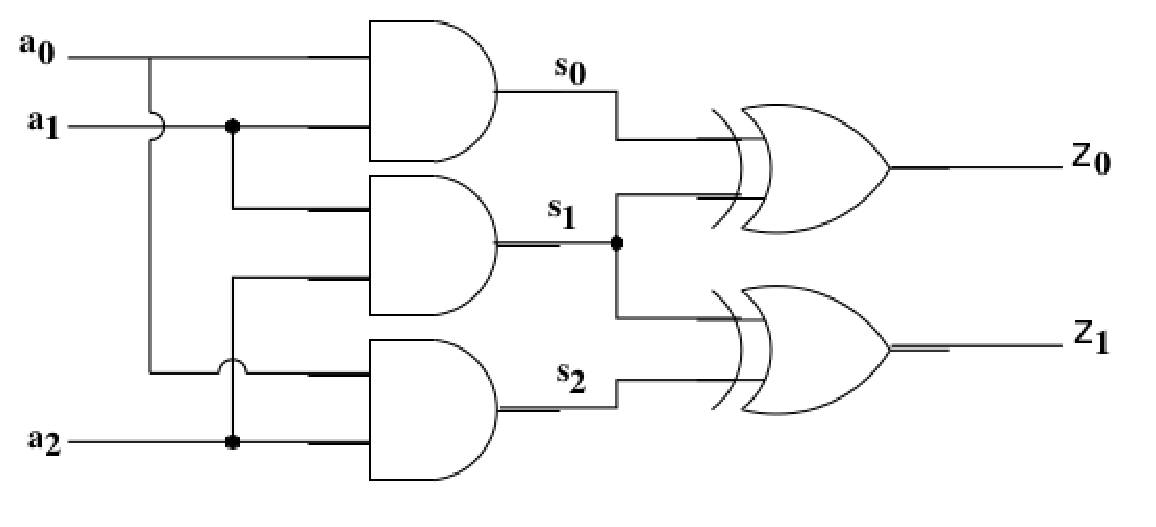
\includegraphics[scale=0.80]{figures/2to3.eps}
	\end{center}
	\caption{Circuit with function $\F_{2^3} \rightarrow \F_{2^2}$}
	\label{fig:2to3fig}
\end{figure}

This circuit has a $3$-bit input $A$ and a $2$-bit output $Z$. Thus, it can
be considered to be a functional mapping over two fields 
$\F_{2^3} \rightarrow \F_{2^2}$. Let $\beta$ be the root of the irreducible 
polynomial $P_k$ of degree $3$ which is generates $\F_{2^3}$. 
Let $\gamma$ be the root of
the irreducible polynomial $P_j$ of degree $2$
which generates $\F_{2^2}$. Then the 
word-level designation polynomials of the input and output, $f_A$ and $f_Z$, 
are:
\begin{eqnarray}
f_A&:&A+a_0+a_1\cdot\beta+a_2\cdot\beta^2 \nonumber \\
f_Z&:&Z+z_0+z_1\cdot\gamma \nonumber
\end{eqnarray}

As $lcm(2,3)=6$, the smallest field that contains both 
$\F_{2^3}$ and $\F_{2^2}$ is $\F_{2^6}$. Thus,
the word-level polynomial $Z+\Func(A)$ is a polynomial over $\F_{2^6}$.
Let $\alpha$ be the root of the 
irreducible polynomial $P_h$ of degree $6$ which generates $\F_{2^6}$. 
Using Theorem \ref{thm:2to3thm}, we find $\beta$ and $\gamma$ in terms of 
$\alpha$, as follows: 
\begin{eqnarray}
\beta=\alpha^\omega, \omega={2^{2\cdot3}-1 \over 2^3-1}=9 \nonumber \\
\gamma=\alpha^\psi, \psi={2^{3\cdot2}-1 \over 2^2-1}=21 \nonumber
\end{eqnarray}
thus, $\beta=\alpha^9$ and $\gamma=\alpha^{21}$. 
The polynomials $f_A$ and $f_Z$ are now be represented as:
\begin{eqnarray}
f_A&:&A+a_0+a_1\cdot\alpha^9+a_2\cdot\alpha^{18} \nonumber \\
f_Z&:&Z+z_0+z_1\cdot\alpha^{21} \nonumber
\end{eqnarray}
We can now analyze the entire circuit over $\F_{2^6}$.
\label{exp:2to3ex1}
\end{Example}

\subsection{Abstraction of Circuits over Different Galois Fields}

With all polynomials modelled over $\F_{2^h}$, we can apply our abstraction
approach using abstraction ordering to find the word-level polynomial
function $Z+\F(A)$ over $\F_{2^h}$, as shown in a previous chapter. Note that
vanishing polynomials for the word-level variables, $A$ and $Z$ are formed 
from their corresponding fields, i.e. $A^{2^k}-A$ and $Z^{2^j}-Z$.

\begin{Example}
Consider the same circuit from Example \ref{exp:2to3ex1}, which performs a
function $\F_{2^3} \rightarrow \F_{2^2}$.
Let $\alpha$ be the root of the irreducible polynomial $P_h=X^6+X+1$, which
is used to construct $\F_{2^6}$.
We model the entire circuit as a system of polynomials $J$ over $\F_{2^6}$.
We find the relevant vanishing polynomials $J_0$. Abstraction ordering of 
this circuit is
\begin{equation}
z_0>z_1>s_0>s_1>s_2>a_0>a_1>a_2>Z>A \nonumber
\end{equation}
The system of polynomials $J+J_0$ is

\begin{eqnarray}\label{eqn:miterbit}
 \left .  \begin{aligned}
f_1&:&s_0+a_0\cdot a_1\nonumber\\
f_2&:&s_1+a_1\cdot a_2\nonumber\\
f_3&:&s_2+a_0\cdot a_2\nonumber\\
f_4&:&z_0+s_0+s_1\nonumber\\
f_5&:&z_1+s_1+s_2\nonumber\\
\end{aligned}
\ \right\}
&\qquad&  \text{\it Bit-level implementation} (J) \nonumber \\
 \left .  \begin{aligned}
f_A&:&a_0+a_1\cdot\alpha^9+a_2\cdot\alpha^{18}+A\nonumber\\
f_Z&:&z_0+z_1\cdot\alpha^{21}+Z\nonumber\\ 
\end{aligned}
\ \right\}
 &\qquad&  \text{\it Word-level designation} (J) \nonumber \\
\left . \begin{aligned}
a_0^2-a_0\nonumber\\
a_1^2-a_1\nonumber\\
a_2^2-a_2\nonumber\\
z_0^2-z_0\nonumber\\
z_1^2-z_1\nonumber\\
s_0^2-s_0\nonumber\\
s_1^2-s_1\nonumber\\
s_2^2-s_2\nonumber\\
A^8-A\nonumber\\
Z^4-Z\nonumber
\end{aligned}
\ \right\}
&\qquad&  \text{\it Vanishing Polynomials} (J_0) \nonumber 
\end{eqnarray}

By computing a reduced \Grobner basis, the word-level abstraction polynomial
in the form of $Z+\Func(A)$ is found in the basis:
\begin{equation}
Z+(\alpha^2+\alpha)A^6+(\alpha^4+\alpha^3+\alpha)A^5+(\alpha^2+\alpha)A^4+(\alpha^4+\alpha^3+\alpha^2)A^3+(\alpha^4+\alpha^3+\alpha^2)A^2+(\alpha^4+\alpha^3+\alpha)A \nonumber
\end{equation}
\end{Example}


This method allows us to abstract a word-level polynomial representation
of circuits which have inputs and outputs of different datapath sizes, where
previously abstraction was only possible if the datapath of the inputs and
outputs was the same.
However, if this circuit with function $\Fkk \rightarrow \F_{2^j}$ does not 
perform a
simple function over the give $\F_{2^h}$, like in the example above, then 
the word-level polynomial representation over $Z+\Func(A)$ over $\F_{2^h}$ 
could be quite large. In this case, our approach to obviate the complexity
of the \Grobner basis computation will derive a representation with bit-level
input variables.
Also, depending on the size of the inputs, $k$, and the 
size of the outputs, $j$, the field $\F_{2^h}$ could be very large if $j$ and
$k$ are relatively prime to each other, i.e. $lcm(j,k)=j*k$.

\section{Conclusions}

In this chapter we proposed two more applications of word-level abstraction 
over Galois Fields: a partitioning algorithm over $\Fkk$ and an approach to
analyze circuits over $\Fkk \rightarrow \F_{2^j}$.
Notably, these proposals are applicable not just to 
abstraction, but to all computer-algebra based formal verification of Galois 
field circuits. Currently, there are a few limitations of these proposals 
when applied to our abstraction approach. When applied to partitions, our 
abstraction approach with obviation of \Grobner basis computation produces a 
result with bit-level input variables. Thus, we cannot apply substitution to
abstract the full representation of the partitioned circuit. However, 
we could potentially apply these mixed-level abstractions to Lv's
equivalence approach, as described in the previous chapter.

There are a number of unexplored applications of the proposals put forth in 
this chapter. If our abstraction approach could guarantee a word-level 
abstraction of any circuit logic, then the partitioning approach could 
very-well allows us to abstract even larger Galois field circuits. Our 
proposal of abstracting representations of circuits over 
$\Fkk \rightarrow \F_{2^j}$ could also then be applied to allow for 
partitions of varying inputs and outputs. These applications seem 
promising, and thus motivate further research.

\chapter{Conclusions and Future Work}
\label{ch:concl}

A combinational circuit with $k$-inputs and $k$-outputs implements
Boolean functions  $f: \B ^k \rightarrow \B ^k$, where $\B = \{0,
1\}$. The function can also be construed as a mapping  $f: \Fkk
\rightarrow \Fkk$, where $\Fkk$ denotes the Galois field of
$2^k$ elements. A circuit with differing input and output sizes 
computes $f: \B ^m \rightarrow \B ^n$, which can be represented
as a function over Galois fields $f: \F_{2^m} \rightarrow \F_{2^n}$.
This circuit can also be analyzed as the function 
$f: \Fkk \rightarrow \Fkk$, where $\Fkk \supset \F_{2^m}$ 
and $\Fkk \supset \F_{2^m}$.

Every function $f$ over $\Fkk$ is a polynomial
function --- i.e., there exists a unique,  minimal, canonical
polynomial $\Func$ that describes $f$. This dissertation presented novel
techniques based on computer-algebra and algebraic-geometry to
derive the canonical (word-level) polynomial representation from the
circuit as  $Z = \Func(A)$ over $\Fkk$, where $A$ and $Z$ denote, 
respectively, the input and output bit-vectors of the circuit.

A theory for word-level polynomial abstraction of bit-level circuits 
over Galois fields is first developed.
This theory is derived using techniques from computer-algebra, notably the theory of
\Grobner basis. However, due to the computational complexity of computing a \Grobner
basis, the solution is not scalable to large designs.
In order to overcome these limitations, new symbolic computational
algorithms are developed and refined. The algorithms employ techniques
from the binomial expansion over $\Fkk$ and $\F_4$-style reduction and can exploit
hierarchy in a given circuit. Finally, an efficient implementation of the algorithmic
approach is presented.

Experiments show that the proposed approach works exceptionally well
for abstracting word-level Galois field arithmetic circuits. It has been
shown that the approach can abstract and verify these types of circuits with up to 
$1024$-bit datapaths. Other contemporary techniques
cannot to verify these types for circuits beyond $163$-bits and fail to
abstract them beyond $32$-bits.

However, in cases of random logic, the abstraction approach
can generate high-degree polynomials:
\begin{equation}
X^{q-1}+X^{q-2}\dots
\end{equation}
In these cases, the polynomials derived during the computation are dense, 
and the computational complexity of manipulating such polynomials
makes abstraction infeasible.

\section{Future Work}

Due to the modular nature of the proposed solution, there are many
potential future research directions that can be explored.

\subsection{Hardware Acceleration}
The first reduction step, $f_Z\xrightarrow{F-f_{z_i},F_0}_+ r$
is the most computationally complex part of the proposed abstraction approach. This
reduction could be implemented using a hardware accelerator.
Significant speed-ups have 
been observed in GPU implementations of circuit simulation algorithms 
\cite{PengLi:GPU}. 
Furthermore, this work has shown cases where multiple, independent abstractions 
need to be computed at the same time, such as when abstracting a word-level 
representation of a composite field multiplier.

These abstractions can be computed in parallel with one another, and this
parallelism could then be exploited using a GPU. Furthermore, our 
approach to compute the abstractions uses an $F4$-style reduction procedure, 
which performs many complex computations over a large matrix. 
Operations over matrices can be suitably implemented using a GPU.
Lastly, the substitution by $a_i=\Func(A)$ is trivially parallelized. 
Thus, further study is proposed to implement word-level abstraction 
on a general purpose GPU.

\subsection{Integration with EDA Tools} 
The proposed canonical word-level abstraction approach is a full, 
self-contained solution.
It can thus be integrated into other EDA tools. There are direct
applications of word-level abstractions to design synthesis. For instance, 
the approach can compute a functional decomposition of a logic or it could 
be used in high-level RTL synthesis. Since the derived abstraction 
is canonical, it can also be used in verification engines such as SMT solvers.
The abstraction approach most efficiently handles AND/XOR logic, so it
could be used to complement approaches in the mentioned tools that are
efficient over AND/OR logic.

\subsection{Polynomial Reductions using Data-Structures}
The abstraction approach poorly handles chains of OR gates
due to their representation as polynomials of Galois fields.
Other polynomial-based tools \cite{polybori:2009} have shown that it 
can be beneficial to represent polynomials internally as decision diagrams.
Thus, it is worthwhile to explore whether it is possible to
implement the algorithmic approach in a different data-structure that
is better-suited for handling this type of logic.
One candidate data-structure is the And-Invert-Graph, as this structure efficiently
handles OR gates. The widely-used tool ABC\cite{abc} provides a very efficient, 
flexible, and open-source implementation of the AIG data structure.

Recall that a one-step reduction  of the polynomial $f$ by polynomial $g$, 
$f\xrightarrow{g} r$, is computed as:
\begin{equation}
r = f-\frac{LT(f)}{LT(g)}\cdot g
\end{equation}
Over Boolean circuits, $\B \equiv \F_2$. Since the leading term of
any monomial in $\B$ is $1$, and $-1\equiv +1$, then
\begin{equation}
f-(\frac{LT(f)}{LT(g)}\cdot g)\equiv f+(\frac{LM(f)}{LM(g)}\cdot g)
\end{equation}
which computes an XOR operation
\begin{equation}
f\oplus(\frac{LM(f)}{LM(g)}\cdot g)
\end{equation}
while the $\cdot$ operator acts as an AND operation $\wedge$.
So one step of the reduction procedure can be computed as the following 
AND/XOR operation:
\begin{equation}
r = f \oplus \frac{LM(f)}{LM(g)}\wedge g
\end{equation}

Thus, we propose an investigation into implementing the algorithms presented
in this dissertation over AIGs.

\subsection{Application to Sequential Circuit Verification}
Sequential Galois field arithmetic circuits over $\Fkk$
take k-bit inputs and produce a k-bit result after k-clock cycles 
of operation. Formal verification of sequential arithmetic
circuits with large datapath sizes is beyond the capabilities of
contemporary verification techniques. To address this problem,
we described a verification method in \cite{sun:date15} 
which uses the presented abstraction approach to implicitly 
unroll the sequential arithmetic circuit over multiple (k) clock-cycles.
The resulting function computed by the state-registers of the circuit 
is represented canonically as a multi-variate word-level polynomial over
$\Fkk$. While directly applicable to sequential Galois field arithmetic circuits, 
this work needs to be further generalized in order to make applicable to
any sequential state machine. 

\subsection{Application to Formal Software Verification}
Computer algebra techniques based on \Grobner basis theory have been used 
in formal software verification \cite{manna:program}.
In this work, a \Grobner basis computation is used to derive {\it loop invariants}.
However, the derived invariants are not bit-precise, so not every invariant that is
computed can be applied to the verification. As our approach maintains
the input-output relationship in the abstraction, it could be applied to
find bit-precise invariants.


\subsection{Application to Integer Arithmetic Circuits}
The abstraction approach derives a
word-level representation of circuits over Galois fields, $\Fkk$. 
In order to expand its usability, we conjecture whether it is possible to 
apply concepts from this approach to {\bf abstract word-level representations 
of circuits over integer rings}, $\Zkk$. 
As any function over a Galois 
field $\Fkk$ is a polynomial function, there exists a polynomial which 
describes the word-level function of a given circuit over $\Fkk$. 
%If the word-level 
%input and output of the circuit is $A$ and $Z$, respectively, this 
%polynomial exists in the form $Z=\Func(A)$.
However, not every function over an integer ring $\Zkk$ is a polynomial 
function. 
Thus, a single polynomial which describes the function of a circuit over 
$\Zkk$ is not guaranteed to exist. 
%Instead, there could exist a set of
%polynomials $\{f_1,\dots,f_n\}$ which describes this function.
%These polynomials are in following form:
%\begin{eqnarray}
%f_1:Z=\Func_1(A) \nonumber \\
%\vdots \nonumber \\
%f_n:Z=\Func_n(A) \nonumber
%\end{eqnarray}
Even though there may not exist a single polynomial which describes the
entire function over $\Zkk$, elimination theory and \Grobner basis still
applies over this ring. Thus, it may be possible to modify the theory and 
implementation of our word-level 
abstraction approach in order to abstract a set of word-level 
polynomials over $\Zkk$.


\begin{center}
{\Large \bf Appendix: Omitted Proofs}
\end{center}


\par \noindent {\bf Proof of Theorem \ref{thm:smallest}.} 
\begin{proof}
Let $J_I \subseteq \Fq[C]$ be any another ideal-interpolant $\neq
J_S$. We show that $\Vc(J_S) \subseteq \Vc(J_I)$. For $\Vc(J_I)$
to be an interpolant it must satisfy 
\begin{align*}
\Vabc(J_A) \subseteq \Vabc(J_I)
\end{align*}
which is equivalent to 
\begin{align*}
I(\Vabc(J_A)) &\supseteq I(\Vabc(J_I)) \\
\implies J_A &\supseteq J_I  
\end{align*}
due to Theorem \ref{thm:strong-ns}.
%% as $J_I$ is radical so $I(\Vabc(J_I)) = J_I)$. 
As the generators of $J_I$ only contain polynomials in $C$-variables,
this relation also holds for the following
\begin{align*}
J_A \cap \Fq[C] &\supseteq J_I \\
\implies J_S &\supseteq J_I \\
\implies \Vc(J_S) &\subseteq \Vc(J_I).
\end{align*} 



\end{proof}

\par \noindent {\bf Proof of Theorem \ref{thm:large}.} 


\begin{proof} 
We first prove that the interpolant computed by
complementing $\Vc(J'_L)$  as $\Fq^C - \Vc(J'_L)$ is indeed a valid
interpolant. As $J'_L$ is the elimination ideal computed from $J_B$,
$\Vbc(J'_L) \supseteq \Vbc(J_B)$. This in turn implies that the
complement of $V(J'_L)$ cannot intersect with $V(J_B)$ at any
point. This proves condition 2 for $\Fq^C - \Vc(J'_L)$ to be a
valid interpolant.  

For condition 1, we need to prove that
\begin{align*}
\Vac(J_A) \subseteq \Fq^A \times (\Fq^C - \Vc(J'_L))
\end{align*}
This can be restated as
\begin{align*}
\Vac(J_A) \cap \Fq^A \times \Vc(J'_L) = \emptyset
\end{align*}
Let us assume (by contradiction) that there exists a common point 
$(\mathbf{a},\mathbf{c})$ in $\Vac(J_A)$ and $\Fq^A \times
V_C(J'_L)$. As the projection $Pr_B(\Vbc(J_B))$ on the
$C$-variables is equal to  the variety of the elimination ideal
$\Vc(J'_L)$, a point $(\mathbf{c}) \in \Vc(J'_L)$ can be  extended to
some point $(\mathbf{b},\mathbf{c})$ in $\Vbc(J_B)$. This implies that
the point $(\mathbf{a},\mathbf{b},\mathbf{c})$ is a common point in
$\Vabc(J_A)$ and $\Vabc(J_B)$, which is a contradiction to our initial
assumption. Therefore condition 1 of Def. \ref{def:int} is satisfied
too and $\Fq^C - \Vc(J'_L)$ is indeed an interpolant. 

\par \noindent Next we prove that $\Fq^C - \Vc(J'_L)$ is the largest
interpolant. Consider an arbitrary ideal-interpolant $J_I$. We want to
prove $\Vc(J_I) \subseteq \Fq^C - \Vc(J'_L)$, or equivalently to prove
$\Vc(J_I) \cap \Vc(J'_L) = \emptyset$. Let us assume (by contradiction) 
that there exists a common point $(\mathbf{c})$ in $\Vc(J_I)$ and
$\Vc(J'_L)$. As $J'_L$ is the elimination ideal of $J_B$, this point
can be extended to some point $(\mathbf{b},\mathbf{c})$  
in $\Vbc(J_B)$. This in turn implies that $(\mathbf{b},\mathbf{c})$ is
a common point in  $\Vbc(J_B)$ and $\Fq^B \times \Vc(J_I)$. This is a
contradiction as an interpolant cannot intersect with the variety of
$J_B$. Hence, $\Fq^C - \Vc(J'_L)$ is the largest interpolant and it
contains all other interpolants.

\end{proof}


\par \noindent {\bf Proof of Lemma \ref{noofinter}.} 
\begin{proof}
The smallest and the largest interpolants are $\Vc(J_S)$ and $\Vc(J_L)$,
respectively. The set difference $\Vc(J_L) - \Vc(J_S)$ is also a
variety of some ideal $J_D$, which can be computed as
$J_D=(J_L:J_S)$. By selecting different subsets of $\Vc(J_D)$ and
adding them to $\Vc(J_S)$, we can generate all the 
interpolants. Consider, 
\begin{align*}
\label{eqn:pwsetjd}
\binom{|\Vc(J_D)|}{0} + \binom{|\Vc(J_D)|}{1} + \cdots + \binom{|\Vc(J_D)|}{|\Vc(J_D)|} = 2^{|\Vc(J_D)|}
\end{align*}
where the term $\binom{|\Vc(J_D)|}{0}$ denotes that no point is selected from $\Vc(J_D)$ and results in 
$\Vc(J_S)$ as the ideal-interpolant. On the other hand, the term $\binom{|\Vc(J_D)|}{|\Vc(J_D)|}$ is equivalent 
to selecting  all the points from $\Vc(J_D)$ and results in $J_L$ as 
the ideal-interpolant. So the number of interpolants is equal to
$2^{|\Vc(J_D)|}$. Theorem \ref{thm:count} further tells us that the 
cardinality of a variety of an ideal is equal to the number of
standard monomials of that ideal, therefore, number of interpolants $=
2^{|SM(J_D)|}$.  

\end{proof}

%\newpage

%%%%%%%%%%%%%%%%%%%% The bibliography %%%%%%%%%%%%%%%%%%%%%%%%%%%%

\bibliographystyle{ieee}
\bibliography{logic}
\end{document}

%%%%%%%%%%%%%%%%%%%%%%%%%%%  End of IEEEsample.tex  %%%%%%%%%%%%%%%%%%%%%%%%%%%
